% Options for packages loaded elsewhere
% Options for packages loaded elsewhere
\PassOptionsToPackage{unicode}{hyperref}
\PassOptionsToPackage{hyphens}{url}
\PassOptionsToPackage{dvipsnames,svgnames,x11names}{xcolor}
%
\documentclass[
  french,
  11pt,
  a4paper,
  DIV=11,
  numbers=noendperiod]{scrreprt}
\usepackage{xcolor}
\usepackage[margin=23mm]{geometry}
\usepackage{amsmath,amssymb}
\setcounter{secnumdepth}{5}
\usepackage{iftex}
\ifPDFTeX
  \usepackage[T1]{fontenc}
  \usepackage[utf8]{inputenc}
  \usepackage{textcomp} % provide euro and other symbols
\else % if luatex or xetex
  \usepackage{unicode-math} % this also loads fontspec
  \defaultfontfeatures{Scale=MatchLowercase}
  \defaultfontfeatures[\rmfamily]{Ligatures=TeX,Scale=1}
\fi
\usepackage{lmodern}
\ifPDFTeX\else
  % xetex/luatex font selection
  \setmainfont[]{DejaVu Serif}
  \setsansfont[]{DejaVu Sans}
  \setmonofont[]{DejaVu Sans Mono}
\fi
% Use upquote if available, for straight quotes in verbatim environments
\IfFileExists{upquote.sty}{\usepackage{upquote}}{}
\IfFileExists{microtype.sty}{% use microtype if available
  \usepackage[]{microtype}
  \UseMicrotypeSet[protrusion]{basicmath} % disable protrusion for tt fonts
}{}
\makeatletter
\@ifundefined{KOMAClassName}{% if non-KOMA class
  \IfFileExists{parskip.sty}{%
    \usepackage{parskip}
  }{% else
    \setlength{\parindent}{0pt}
    \setlength{\parskip}{6pt plus 2pt minus 1pt}}
}{% if KOMA class
  \KOMAoptions{parskip=half}}
\makeatother
% Make \paragraph and \subparagraph free-standing
\makeatletter
\ifx\paragraph\undefined\else
  \let\oldparagraph\paragraph
  \renewcommand{\paragraph}{
    \@ifstar
      \xxxParagraphStar
      \xxxParagraphNoStar
  }
  \newcommand{\xxxParagraphStar}[1]{\oldparagraph*{#1}\mbox{}}
  \newcommand{\xxxParagraphNoStar}[1]{\oldparagraph{#1}\mbox{}}
\fi
\ifx\subparagraph\undefined\else
  \let\oldsubparagraph\subparagraph
  \renewcommand{\subparagraph}{
    \@ifstar
      \xxxSubParagraphStar
      \xxxSubParagraphNoStar
  }
  \newcommand{\xxxSubParagraphStar}[1]{\oldsubparagraph*{#1}\mbox{}}
  \newcommand{\xxxSubParagraphNoStar}[1]{\oldsubparagraph{#1}\mbox{}}
\fi
\makeatother


\usepackage{longtable,booktabs,array}
\newcounter{none} % for unnumbered tables
\usepackage{calc} % for calculating minipage widths
% Correct order of tables after \paragraph or \subparagraph
\usepackage{etoolbox}
\makeatletter
\patchcmd\longtable{\par}{\if@noskipsec\mbox{}\fi\par}{}{}
\makeatother
% Allow footnotes in longtable head/foot
\IfFileExists{footnotehyper.sty}{\usepackage{footnotehyper}}{\usepackage{footnote}}
\makesavenoteenv{longtable}
\usepackage{graphicx}
\makeatletter
\newsavebox\pandoc@box
\newcommand*\pandocbounded[1]{% scales image to fit in text height/width
  \sbox\pandoc@box{#1}%
  \Gscale@div\@tempa{\textheight}{\dimexpr\ht\pandoc@box+\dp\pandoc@box\relax}%
  \Gscale@div\@tempb{\linewidth}{\wd\pandoc@box}%
  \ifdim\@tempb\p@<\@tempa\p@\let\@tempa\@tempb\fi% select the smaller of both
  \ifdim\@tempa\p@<\p@\scalebox{\@tempa}{\usebox\pandoc@box}%
  \else\usebox{\pandoc@box}%
  \fi%
}
% Set default figure placement to htbp
\def\fps@figure{htbp}
\makeatother


% definitions for citeproc citations
\NewDocumentCommand\citeproctext{}{}
\NewDocumentCommand\citeproc{mm}{%
  \begingroup\def\citeproctext{#2}\cite{#1}\endgroup}
\makeatletter
 % allow citations to break across lines
 \let\@cite@ofmt\@firstofone
 % avoid brackets around text for \cite:
 \def\@biblabel#1{}
 \def\@cite#1#2{{#1\if@tempswa , #2\fi}}
\makeatother
\newlength{\cslhangindent}
\setlength{\cslhangindent}{1.5em}
\newlength{\csllabelwidth}
\setlength{\csllabelwidth}{3em}
\newenvironment{CSLReferences}[2] % #1 hanging-indent, #2 entry-spacing
 {\begin{list}{}{%
  \setlength{\itemindent}{0pt}
  \setlength{\leftmargin}{0pt}
  \setlength{\parsep}{0pt}
  % turn on hanging indent if param 1 is 1
  \ifodd #1
   \setlength{\leftmargin}{\cslhangindent}
   \setlength{\itemindent}{-1\cslhangindent}
  \fi
  % set entry spacing
  \setlength{\itemsep}{#2\baselineskip}}}
 {\end{list}}
\usepackage{calc}
\newcommand{\CSLBlock}[1]{\hfill\break\parbox[t]{\linewidth}{\strut\ignorespaces#1\strut}}
\newcommand{\CSLLeftMargin}[1]{\parbox[t]{\csllabelwidth}{\strut#1\strut}}
\newcommand{\CSLRightInline}[1]{\parbox[t]{\linewidth - \csllabelwidth}{\strut#1\strut}}
\newcommand{\CSLIndent}[1]{\hspace{\cslhangindent}#1}

\ifLuaTeX
\usepackage[bidi=basic,shorthands=off]{babel}
\else
\usepackage[bidi=default,shorthands=off]{babel}
\fi
\ifPDFTeX
\else
\babelfont{rm}[]{DejaVu Serif}
\fi
\ifLuaTeX
  \usepackage{selnolig} % disable illegal ligatures
\fi


\setlength{\emergencystretch}{3em} % prevent overfull lines

\providecommand{\tightlist}{%
  \setlength{\itemsep}{0pt}\setlength{\parskip}{0pt}}



 


\usepackage{eso-pic}
\usepackage{needspace}
\usepackage{etoolbox}
\AtBeginEnvironment{longtable}{\small\setlength{\tabcolsep}{4pt}}
\setlength{\emergencystretch}{3em}
\setkomafont{disposition}{\normalfont\sffamily\bfseries}
\RedeclareSectionCommand[beforeskip=0pt,afterskip=1.2\baselineskip]{chapter}

\RedeclareSectionCommand[beforeskip=.9\baselineskip,afterskip=.45\baselineskip]{section}

% Éviter l'interprétation des lettres d'annexes comme numéros de parties.
\AtEndPreamble{\ifdefined\frenchsetup\frenchsetup{TocPartNameFull=false}\fi}

\DeclareTOCStyleEntry[numwidth=2.5em]{tocline}{chapter}
\KOMAoption{captions}{tableheading}
\makeatletter
\@ifpackageloaded{tcolorbox}{}{\usepackage[skins,breakable]{tcolorbox}}
\@ifpackageloaded{fontawesome5}{}{\usepackage{fontawesome5}}
\definecolor{quarto-callout-color}{HTML}{909090}
\definecolor{quarto-callout-note-color}{HTML}{0758E5}
\definecolor{quarto-callout-important-color}{HTML}{CC1914}
\definecolor{quarto-callout-warning-color}{HTML}{EB9113}
\definecolor{quarto-callout-tip-color}{HTML}{00A047}
\definecolor{quarto-callout-caution-color}{HTML}{FC5300}
\definecolor{quarto-callout-color-frame}{HTML}{acacac}
\definecolor{quarto-callout-note-color-frame}{HTML}{4582ec}
\definecolor{quarto-callout-important-color-frame}{HTML}{d9534f}
\definecolor{quarto-callout-warning-color-frame}{HTML}{f0ad4e}
\definecolor{quarto-callout-tip-color-frame}{HTML}{02b875}
\definecolor{quarto-callout-caution-color-frame}{HTML}{fd7e14}
\makeatother
\makeatletter
\@ifpackageloaded{bookmark}{}{\usepackage{bookmark}}
\makeatother
\makeatletter
\@ifpackageloaded{caption}{}{\usepackage{caption}}
\AtBeginDocument{%
\ifdefined\contentsname
  \renewcommand*\contentsname{Table des matières}
\else
  \newcommand\contentsname{Table des matières}
\fi
\ifdefined\listfigurename
  \renewcommand*\listfigurename{Liste des Figures}
\else
  \newcommand\listfigurename{Liste des Figures}
\fi
\ifdefined\listtablename
  \renewcommand*\listtablename{Liste des Tables}
\else
  \newcommand\listtablename{Liste des Tables}
\fi
\ifdefined\figurename
  \renewcommand*\figurename{Figure}
\else
  \newcommand\figurename{Figure}
\fi
\ifdefined\tablename
  \renewcommand*\tablename{Table}
\else
  \newcommand\tablename{Table}
\fi
}
\@ifpackageloaded{float}{}{\usepackage{float}}
\floatstyle{ruled}
\@ifundefined{c@chapter}{\newfloat{codelisting}{h}{lop}}{\newfloat{codelisting}{h}{lop}[chapter]}
\floatname{codelisting}{Listing}
\newcommand*\listoflistings{\listof{codelisting}{Liste des Listings}}
\makeatother
\makeatletter
\makeatother
\makeatletter
\@ifpackageloaded{caption}{}{\usepackage{caption}}
\@ifpackageloaded{subcaption}{}{\usepackage{subcaption}}
\makeatother
\usepackage{bookmark}
\IfFileExists{xurl.sty}{\usepackage{xurl}}{} % add URL line breaks if available
\urlstyle{same}
\hypersetup{
  pdftitle={Analyse factorielle confirmatoire},
  pdfauthor={Daniel Coulombe},
  pdflang={fr},
  colorlinks=true,
  linkcolor={blue},
  filecolor={Maroon},
  citecolor={Blue},
  urlcolor={Blue},
  pdfcreator={LaTeX via pandoc}}


\title{Analyse factorielle confirmatoire}
\usepackage{etoolbox}
\makeatletter
\providecommand{\subtitle}[1]{% add subtitle to \maketitle
  \apptocmd{\@title}{\par {\large #1 \par}}{}{}
}
\makeatother
\subtitle{Comprendre et pratiquer avec l'application CFA}
\author{Daniel Coulombe}
\date{20 novembre 2026}
\begin{document}
\maketitle

% Couverture pleine page ; le titre normal demeure disponible comme page de titre.
\begin{titlepage}
\thispagestyle{empty}
\AddToShipoutPictureBG*{\AtPageLowerLeft{
\includegraphics[width=\paperwidth,height=\paperheight]{cover.png}}}
\null
\end{titlepage}

\renewcommand*\contentsname{Table des matières}
{
\setcounter{tocdepth}{0}
\tableofcontents
}

\bookmarksetup{startatroot}

\chapter*{Bienvenue}\label{bienvenue}
\addcontentsline{toc}{chapter}{Bienvenue}

\markboth{Bienvenue}{Bienvenue}

Ce manuel accompagne l'\textbf{application CFA} pour apprendre à
spécifier, estimer et interpréter une analyse factorielle confirmatoire,
ou \textbf{AFC}. Le point de départ est une question de mesure :
plusieurs réponses ou performances peuvent-elles être représentées par
les dimensions que nous souhaitons mesurer ? Le résultat recherché est
une conclusion argumentée sur un modèle de mesure, appuyée sur les
données, les paramètres et les limites de l'analyse.

Le logiciel accomplit les calculs. Votre travail consiste à définir ce
que les variables représentent, à choisir une analyse cohérente avec
leur nature, à vérifier la solution et à expliquer ce que les résultats
permettent de soutenir. Un modèle peut converger, donner des
coefficients significatifs et demeurer substantiellement discutable.

\section*{Ce qu'il faut pour
commencer}\label{ce-quil-faut-pour-commencer}
\addcontentsline{toc}{section}{Ce qu'il faut pour commencer}

\markright{Ce qu'il faut pour commencer}

Ouvrez l'application CFA fournie dans votre cours et gardez ce manuel
dans une autre fenêtre. \textbf{Aucune connaissance de R, aucune saisie
de syntaxe et aucune installation d'un package ne sont requises pour les
activités du lecteur.} L'application peut être utilisée en ligne ou dans
l'environnement préparé par votre enseignant. Si une session se ferme,
conservez les rapports déjà téléchargés : ils permettent de retrouver
les analyses réalisées.

Les préalables utiles sont la moyenne, la variance, la corrélation, la
régression simple, l'intervalle de confiance et le test d'hypothèse. Le
premier chapitre rappelle leur rôle dans le modèle de mesure. On ne
suppose pas que vous connaissiez déjà les variables latentes, les
estimateurs robustes ou la fiabilité fondée sur un modèle.

Les intitulés cités en \textbf{gras} correspondent aux commandes de
l'application. Les valeurs numériques du manuel ne sont pas recopiées :
elles sont calculées à chaque compilation par le moteur même de
l'application, sur les fichiers et les réglages indiqués (cette édition
: lavaan 0.7.3, R version 4.5.1). Les dernières décimales peuvent varier
avec la version du moteur de calcul. Une différence plus importante doit
conduire à vérifier les données, le modèle, l'estimateur et les cas
utilisés.

\section*{Où trouver les données}\label{ouxf9-trouver-les-donnuxe9es}
\addcontentsline{toc}{section}{Où trouver les données}

\markright{Où trouver les données}

Les sept exemples réels sont directement accessibles dans \textbf{1.
Choisir les données → Données réelles}. Sélectionnez un jeu pour lire sa
fiche. Le bouton \textbf{Charger cet exemple et son modèle} prépare les
facteurs, leurs indicateurs et les réglages proposés. Les boutons
\textbf{Données CSV} et \textbf{Notice et modèle} permettent de
conserver les fichiers sur votre ordinateur. Il n'est pas nécessaire
d'accéder au code de l'application ou du manuel.

Un exercice sur les données manquantes utilise un fichier dérivé,
clairement identifié comme pédagogique. Il est fourni dans le complément
\textbf{CFA\_donnees\_et\_activites.zip} à distribuer avec le manuel.
Une méthode pour le reconstruire à partir du téléchargement de
l'application est également donnée. Si vous lisez le PDF ou l'EPUB,
utilisez l'application pour les données originales et le complément
distribué par votre cours pour ce fichier dérivé. Ne cherchez pas un
dossier de code auquel vous n'auriez pas accès.

\section*{Trois parcours possibles}\label{trois-parcours-possibles}
\addcontentsline{toc}{section}{Trois parcours possibles}

\markright{Trois parcours possibles}

\Needspace{7\baselineskip}

{\def\LTcaptype{none} % do not increment counter
\begin{longtable}[]{@{}
  >{\raggedright\arraybackslash}p{(\linewidth - 2\tabcolsep) * \real{0.5000}}
  >{\raggedright\arraybackslash}p{(\linewidth - 2\tabcolsep) * \real{0.5000}}@{}}
\toprule\noalign{}
\begin{minipage}[b]{\linewidth}\raggedright
Votre objectif
\end{minipage} & \begin{minipage}[b]{\linewidth}\raggedright
Parcours conseillé
\end{minipage} \\
\midrule\noalign{}
\endhead
\bottomrule\noalign{}
\endlastfoot
Réaliser une première AFC & Lire les chapitres sur la mesure et
l'interface, puis suivre intégralement la première analyse \\
Comprendre les résultats & Poursuivre avec l'ajustement, les
diagnostics, la fiabilité et la distinction entre facteurs \\
Conduire une analyse autonome & Ajouter les données ordinales, les
absences, les comparaisons, la simulation et l'étude complète \\
\end{longtable}
}

Les durées dépendent des préalables. Comptez environ une séance pour la
première analyse et plusieurs séances pour traiter sérieusement les
diagnostics et les ateliers. Les exercices avancés ne sont pas des
prérequis cachés des premières manipulations.

\section*{Comment chaque chapitre est
organisé}\label{comment-chaque-chapitre-est-organisuxe9}
\addcontentsline{toc}{section}{Comment chaque chapitre est organisé}

\markright{Comment chaque chapitre est organisé}

Chaque chapitre s'ouvre sur ses \textbf{objectifs} et son \textbf{idée
centrale}. Les captures d'écran montrent l'application dans l'état
décrit par le texte. Un \textbf{laboratoire} propose ensuite une
manipulation guidée, dont la réponse est repliée : essayez avant de
l'ouvrir. Un encadré \textbf{À retenir} et un court \textbf{quiz}, avec
réponses repliées, terminent le chapitre. Dans le PDF, les réponses
apparaissent directement à la suite des questions.

\section*{Comment travailler seul}\label{comment-travailler-seul}
\addcontentsline{toc}{section}{Comment travailler seul}

\markright{Comment travailler seul}

Pour chaque activité, commencez par identifier les données, la question
et les réglages. Faites ensuite les manipulations dans l'ordre. Notez
les résultats avant de lire le corrigé. Lorsque votre résultat diffère
du repère, utilisez les vérifications proposées plutôt que de modifier
des options au hasard.

Un dossier de travail simple suffit : placez-y les CSV téléchargés, les
notices et les rapports HTML. Donnez aux rapports des noms qui
distinguent les analyses, par exemple
\texttt{HS\_trois\_facteurs\_ML.html}. Le navigateur peut ajouter un
suffixe si un fichier de même nom existe déjà : renommez-le au besoin
après le téléchargement.

\section*{Portée de cette édition}\label{portuxe9e-de-cette-uxe9dition}
\addcontentsline{toc}{section}{Portée de cette édition}

\markright{Portée de cette édition}

Le manuel décrit la version de l'application révisée le \textbf{20
novembre 2026} : quatre étapes, deux modes d'affichage, sept jeux réels
et traitement explicite des indicateurs ordinaux. Il porte sur les
modèles de mesure de premier ordre à un groupe que l'interface permet
effectivement de construire. Les modèles structurels de médiation, les
analyses multigroupes, les modèles longitudinaux et les modèles
multiniveaux ne font pas partie des activités proposées ici.

Cette limite ne diminue pas la portée de l'AFC. Elle permet de commencer
par une question essentielle : \textbf{la manière dont nous mesurons les
construits est-elle défendable ?}

\bookmarksetup{startatroot}

\chapter{Mesurer une dimension que l'on n'observe pas
directement}\label{sec-mesurer}

\begin{tcolorbox}[enhanced jigsaw, arc=.35mm, bottomrule=.15mm, bottomtitle=1mm, breakable, colback=white, colbacktitle=quarto-callout-note-color!10!white, colframe=quarto-callout-note-color-frame, coltitle=black, left=2mm, leftrule=.75mm, opacityback=0, opacitybacktitle=0.6, rightrule=.15mm, title={Objectifs du chapitre}, titlerule=0mm, toprule=.15mm, toptitle=1mm]

\begin{itemize}
\tightlist
\item
  Distinguer un indicateur, un score calculé, un facteur et un score
  factoriel.
\item
  Écrire l'équation d'un indicateur continu et décomposer sa variance.
\item
  Comprendre pourquoi un facteur doit recevoir une échelle par
  convention.
\item
  Compter les degrés de liberté d'un modèle et savoir ce que ce compte
  ne garantit pas.
\end{itemize}

\end{tcolorbox}

\begin{tcolorbox}[enhanced jigsaw, arc=.35mm, bottomrule=.15mm, bottomtitle=1mm, breakable, colback=white, colbacktitle=quarto-callout-tip-color!10!white, colframe=quarto-callout-tip-color-frame, coltitle=black, left=2mm, leftrule=.75mm, opacityback=0, opacitybacktitle=0.6, rightrule=.15mm, title={Idée centrale}, titlerule=0mm, toprule=.15mm, toptitle=1mm]

Une AFC traduit une hypothèse de mesure en une structure de covariances.
Le modèle dit d'où viennent les relations entre les réponses : d'un
facteur commun, d'un lien entre facteurs ou d'un lien résiduel.
L'analyse examine si les données sont compatibles avec cette
explication.

\end{tcolorbox}

\section{D'une question substantielle à un
modèle}\label{dune-question-substantielle-uxe0-un-moduxe8le}

Supposons que nous voulions mesurer l'engagement dans une formation.
Nous pouvons observer des réponses à des questions sur l'intérêt,
l'effort et la persévérance. Nous ne voyons pas directement une quantité
appelée « engagement ». Nous proposons qu'une dimension commune
contribue aux réponses. Cette dimension est une \textbf{variable
latente}, ou un \textbf{facteur}; les réponses sont ses
\textbf{indicateurs}.

L'AFC commence par une organisation explicite des indicateurs. Dire que
trois items mesurent l'intérêt et que trois autres mesurent l'effort
constitue une hypothèse différente de celle d'un facteur unique. Ces
hypothèses impliquent des structures différentes de covariances.
L'analyse cherche dans quelle mesure les données sont compatibles avec
la structure annoncée.

Le mot \emph{confirmatoire} ne signifie pas que le logiciel confirme
automatiquement la théorie. Il signifie que la structure à examiner est
spécifiée avant l'estimation. Une structure choisie après de nombreuses
modifications sur les mêmes données conserve une dimension exploratoire,
même si elle est estimée par une AFC (\citeproc{ref-bollen1989}{Bollen
1989}; \citeproc{ref-brown2015}{Brown 2015}).

\section{Indicateur et facteur ne sont pas
interchangeables}\label{indicateur-et-facteur-ne-sont-pas-interchangeables}

Un indicateur possède une colonne dans le fichier. Un facteur est défini
par un ensemble de relations avec des indicateurs. Une moyenne d'items
est un score observé calculé; ce n'est pas le facteur latent lui-même.
Un score factoriel est une estimation individuelle dérivée du modèle; il
n'est pas non plus une observation directe du facteur.

\Needspace{8\baselineskip}

{\def\LTcaptype{none} % do not increment counter
\begin{longtable}[]{@{}
  >{\raggedright\arraybackslash}p{(\linewidth - 4\tabcolsep) * \real{0.3333}}
  >{\raggedright\arraybackslash}p{(\linewidth - 4\tabcolsep) * \real{0.3333}}
  >{\raggedright\arraybackslash}p{(\linewidth - 4\tabcolsep) * \real{0.3333}}@{}}
\toprule\noalign{}
\begin{minipage}[b]{\linewidth}\raggedright
Objet
\end{minipage} & \begin{minipage}[b]{\linewidth}\raggedright
Exemple
\end{minipage} & \begin{minipage}[b]{\linewidth}\raggedright
Statut
\end{minipage} \\
\midrule\noalign{}
\endhead
\bottomrule\noalign{}
\endlastfoot
Indicateur & Réponse à l'item « je poursuis malgré les difficultés » &
Valeur observée \\
Score de somme ou de moyenne & Moyenne de quatre réponses & Calcul sur
les réponses \\
Facteur & Persévérance commune aux indicateurs & Variable latente du
modèle \\
Score factoriel & Estimation de la persévérance d'une personne &
Prédiction dépendant du modèle \\
\end{longtable}
}

Cette distinction compte pour l'interprétation des corrélations et de la
fiabilité. Une corrélation entre deux moyennes d'items et une
corrélation entre deux facteurs ne répondent pas exactement à la même
question.

\section{L'équation d'un indicateur
continu}\label{luxe9quation-dun-indicateur-continu}

Dans un modèle simple, l'indicateur \(X_i\) s'écrit :

\[X_i = \nu_i + \lambda_i F + \varepsilon_i.\]

\(\nu_i\) est l'intercept, \(\lambda_i\) la \textbf{saturation} et
\(\varepsilon_i\) le \textbf{résidu}. La saturation indique comment la
valeur attendue de l'indicateur varie avec le facteur. Le résidu
représente la partie de l'indicateur que le facteur n'explique pas. Il
peut comprendre de l'erreur de mesure, des spécificités du contenu ou
d'autres influences non représentées.

On ne doit donc pas lire « résidu » comme synonyme d'« erreur de saisie
». Une variance résiduelle importante peut révéler que l'indicateur
possède une composante spécifique substantielle.

\begin{figure}[htbp]

\centering{

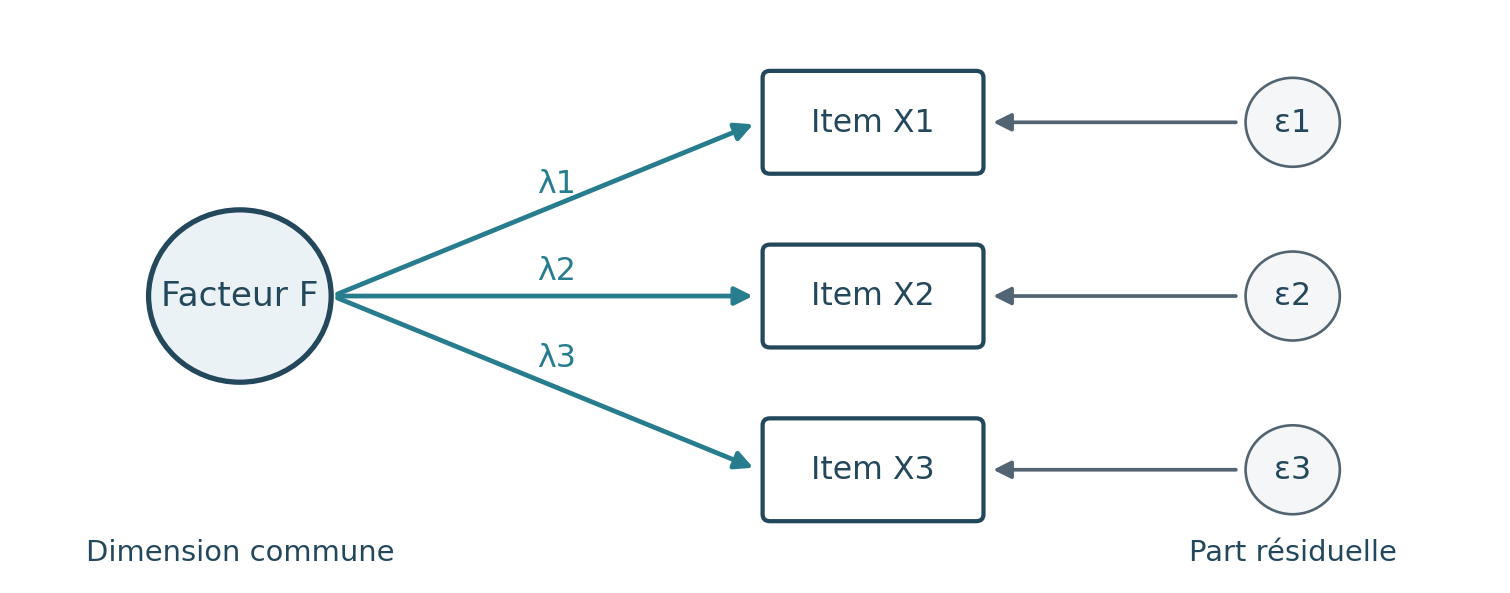
\includegraphics[width=0.8\linewidth,height=\textheight,keepaspectratio]{images/modele_simple.png}

}

\caption{\label{fig-mesure}Un facteur commun contribue à trois
indicateurs; chaque indicateur conserve une partie résiduelle. Schéma
pédagogique.}

\end{figure}%

Dans une structure simple, avec un facteur non corrélé aux résidus, la
variance de l'indicateur se décompose ainsi :

\[\operatorname{Var}(X_i)=\lambda_i^2\operatorname{Var}(F)+\theta_{ii}.\]

Lorsque l'indicateur et le facteur sont standardisés et que l'indicateur
ne mesure qu'un facteur, une saturation de \(0{,}70\) correspond à une
proportion expliquée de \(0{,}70^2=0{,}49\). Environ 49 \% de la
variance de cet indicateur est alors attribuée à ce facteur dans le
modèle. Ce raisonnement ne doit pas être transposé sans précaution à une
structure complexe ou à la somme des catégories d'un item ordinal.

\section{Ce que le modèle explique entre les
variables}\label{ce-que-le-moduxe8le-explique-entre-les-variables}

Deux indicateurs associés au même facteur partagent de la variance. Avec
des résidus non corrélés :

\[\operatorname{Cov}(X_i,X_j)=\lambda_i\lambda_j\operatorname{Var}(F).\]

Si deux indicateurs dépendent de facteurs différents, leur covariance
dépend aussi du lien entre ces facteurs :
\(\operatorname{Cov}(X_i,X_j)=\lambda_i\lambda_j\operatorname{Cov}(F_1,F_2)\).
Une \textbf{covariance résiduelle} ajoute une source de relation qui
n'est pas expliquée par les facteurs. Elle peut se justifier, par
exemple, par un libellé commun ou une méthode de mesure partagée. Elle
ne doit pas servir à absorber sans explication tous les écarts entre le
modèle et les données.

L'écriture d'ensemble est
\(\Sigma=\Lambda\Phi\Lambda^{\mathsf T}+\Theta\). Cette équation
signifie simplement : la covariance prédite entre les indicateurs
combine la partie portée par les facteurs et la partie résiduelle. Vous
n'avez pas à saisir cette équation dans l'application.

\begin{figure}[htbp]

\centering{

\includegraphics[width=0.88\linewidth,height=\textheight,keepaspectratio]{01-mesurer_files/figure-pdf/fig-reproduction-1.png}

}

\caption{\label{fig-reproduction}Avec des saturations standardisées de
0,80, 0,70 et 0,60 sur un même facteur, la corrélation prédite entre
deux indicateurs est le produit de leurs saturations. Le modèle n'a pas
de paramètre propre à chaque paire : il « explique » les trois
corrélations avec trois saturations.}

\end{figure}%

\section{Donner une échelle au
facteur}\label{donner-une-uxe9chelle-au-facteur}

Le facteur n'a pas d'unité naturelle directement observée. L'application
propose deux conventions d'identification : \textbf{λ₁=1}, qui fixe à 1
la saturation d'un indicateur de référence, et \textbf{σ²(F)=1}, qui
fixe la variance du facteur à 1. Une convention est indispensable; elle
ne constitue pas une découverte empirique.

Avec l'indicateur de référence, le facteur est exprimé dans une unité
liée à cet indicateur. La saturation fixée à 1 n'est ni une corrélation
parfaite ni la preuve que cet indicateur est le meilleur. Elle n'est pas
estimée librement et son absence de test de significativité est normale.

Changer correctement de convention peut modifier les coefficients non
standardisés et les variances factorielles sans modifier les covariances
reproduites ni l'ajustement global. L'interprétation des coefficients
standardisés aide à comparer les résultats obtenus sous ces conventions.
Le chapitre suivant le vérifie sur des données réelles : entre les deux
conventions, les saturations standardisées du modèle de référence
diffèrent au plus de 0,000001.

Le \textbf{sens} du facteur dépend aussi de son orientation. Si l'on
renverse simultanément le signe des relations d'un facteur, on peut
obtenir une représentation équivalente. Une saturation négative doit
donc être examinée en tenant compte du contenu et du codage de l'item,
ainsi que de l'orientation des autres indicateurs.

\section{Identification et degrés de
liberté}\label{identification-et-degruxe9s-de-libertuxe9}

Un modèle est identifiable lorsque les paramètres visés peuvent être
déterminés à partir des informations disponibles, sous les contraintes
posées. Avoir un nombre positif de degrés de liberté est une condition
de comptage utile, mais ne prouve pas à elle seule l'identification.

Pour \(p\) indicateurs continus, il existe \(p(p+1)/2\) variances et
covariances distinctes. Avec neuf indicateurs, on en compte
\(9\times10/2=45\). Le modèle usuel à trois facteurs et trois
indicateurs par facteur comporte 21 paramètres de covariance libres :
six saturations, neuf variances résiduelles, trois variances
factorielles et trois covariances factorielles. On obtient donc
\(45-21=24\) degrés de liberté, sous l'identification par indicateur de
référence et sans covariance résiduelle ajoutée. L'application affiche
ce même nombre de paramètres libres dans le bandeau qui suit
l'estimation.

\Needspace{8\baselineskip}

{\def\LTcaptype{none} % do not increment counter
\begin{longtable}[]{@{}lrrr@{}}
\toprule\noalign{}
Modèle & Moments distincts & Paramètres libres & Degrés de liberté \\
\midrule\noalign{}
\endhead
\bottomrule\noalign{}
\endlastfoot
1 facteur, 3 indicateurs & 6 & 6 & 0 \\
1 facteur, 4 indicateurs & 10 & 8 & 2 \\
3 facteurs, 3 indicateurs chacun & 45 & 21 & 24 \\
1 facteur, 9 indicateurs & 45 & 18 & 27 \\
\end{longtable}
}

Un facteur mesuré par trois indicateurs continus, avec les contraintes
usuelles et sans autre restriction, possède zéro degré de liberté. Il
peut reproduire exactement les covariances sans soumettre cette
structure à un test global informatif. Un ajustement parfait dans ce cas
ne constitue pas une validation.

Deux indicateurs par facteur ne donnent pas automatiquement un modèle
identifiable. L'application peut permettre la saisie, mais
l'identification dépend de l'ensemble du modèle et des restrictions.
Pour les premières activités, utilisez les structures fournies.

\begin{tcolorbox}[enhanced jigsaw, arc=.35mm, bottomrule=.15mm, bottomtitle=1mm, breakable, colback=white, colbacktitle=quarto-callout-note-color!10!white, colframe=quarto-callout-note-color-frame, coltitle=black, left=2mm, leftrule=.75mm, opacityback=0, opacitybacktitle=0.6, rightrule=.15mm, title={Dans l'application}, titlerule=0mm, toprule=.15mm, toptitle=1mm]

L'onglet \textbf{Introduction} de la configuration rappelle ces notions
dans \textbf{Concepts de base}, \textbf{Équations} et \textbf{Séquence
d'analyse}. Il ne lance aucun calcul. Le bandeau qui apparaît après
chaque estimation indique l'effectif utilisé et le nombre de paramètres
libres : comparez-le à votre propre compte.

\end{tcolorbox}

\section{Laboratoire : compter avant
d'estimer}\label{laboratoire-compter-avant-destimer}

Sans ouvrir l'application, complétez le compte pour deux modèles
construits sur les six premiers tests de Holzinger--Swineford.

\begin{enumerate}
\def\labelenumi{\arabic{enumi}.}
\tightlist
\item
  Un facteur unique mesuré par \texttt{x1} à \texttt{x6}, identification
  \textbf{λ₁=1}.
\item
  Deux facteurs corrélés, \texttt{x1}--\texttt{x3} et
  \texttt{x4}--\texttt{x6}, même identification.
\end{enumerate}

Pour chacun, calculez les moments distincts, les paramètres libres et
les degrés de liberté. Dites ensuite lequel des deux modèles impose le
plus de restrictions aux données.

\begin{tcolorbox}[enhanced jigsaw, arc=.35mm, bottomrule=.15mm, bottomtitle=1mm, breakable, colback=white, colbacktitle=quarto-callout-tip-color!10!white, colframe=quarto-callout-tip-color-frame, coltitle=black, left=2mm, leftrule=.75mm, opacityback=0, opacitybacktitle=0.6, rightrule=.15mm, title={Réponse}, titlerule=0mm, toprule=.15mm, toptitle=1mm]

Six indicateurs donnent \(6\times7/2=21\) moments distincts.

\begin{enumerate}
\def\labelenumi{\arabic{enumi}.}
\tightlist
\item
  Un facteur : cinq saturations libres, six variances résiduelles et une
  variance factorielle, soit 12 paramètres et \(21-12=9\) degrés de
  liberté.
\item
  Deux facteurs : quatre saturations libres, six variances résiduelles,
  deux variances factorielles et une covariance, soit 13 paramètres et 8
  degrés de liberté.
\end{enumerate}

Le modèle à un facteur impose une restriction de plus : il revient à
fixer à 1 la corrélation entre les deux facteurs du second modèle. Ce
cas limite explique pourquoi le chapitre sur l'ajustement déconseille de
comparer ces deux modèles par une simple différence de chi carré.

\end{tcolorbox}

\begin{tcolorbox}[enhanced jigsaw, arc=.35mm, bottomrule=.15mm, bottomtitle=1mm, breakable, colback=white, colbacktitle=quarto-callout-important-color!10!white, colframe=quarto-callout-important-color-frame, coltitle=black, left=2mm, leftrule=.75mm, opacityback=0, opacitybacktitle=0.6, rightrule=.15mm, title={À retenir}, titlerule=0mm, toprule=.15mm, toptitle=1mm]

\begin{itemize}
\tightlist
\item
  Un facteur est défini par ses relations avec des indicateurs; une
  moyenne d'items et un score factoriel n'en sont que des
  approximations.
\item
  La saturation standardisée au carré donne la part de variance d'un
  indicateur attribuée à son facteur, dans une structure simple.
\item
  La convention d'échelle (λ₁=1 ou σ²(F)=1) change les coefficients non
  standardisés, pas l'ajustement.
\item
  Des degrés de liberté positifs sont nécessaires pour tester une
  structure, mais ne garantissent pas l'identification.
\end{itemize}

\end{tcolorbox}

\section{Quiz}\label{quiz}

\begin{enumerate}
\def\labelenumi{\arabic{enumi}.}
\tightlist
\item
  Pourquoi une saturation fixée à 1 ne prouve-t-elle pas une mesure
  parfaite ?
\item
  Une variance résiduelle importante désigne-t-elle nécessairement une
  erreur accidentelle ?
\item
  Pourquoi une moyenne d'items n'est-elle pas une variable latente ?
\item
  Un modèle à un facteur et trois indicateurs s'ajuste parfaitement.
  Qu'en conclure ?
\end{enumerate}

\begin{tcolorbox}[enhanced jigsaw, arc=.35mm, bottomrule=.15mm, bottomtitle=1mm, breakable, colback=white, colbacktitle=quarto-callout-tip-color!10!white, colframe=quarto-callout-tip-color-frame, coltitle=black, left=2mm, leftrule=.75mm, opacityback=0, opacitybacktitle=0.6, rightrule=.15mm, title={Réponses}, titlerule=0mm, toprule=.15mm, toptitle=1mm]

\begin{enumerate}
\def\labelenumi{\arabic{enumi}.}
\tightlist
\item
  La valeur 1 est une convention d'échelle : elle n'est pas estimée et
  ne mesure pas la qualité de l'indicateur.
\item
  Non. Le résidu peut contenir une spécificité réelle du contenu ou de
  la méthode.
\item
  La moyenne est calculée directement sur les réponses; elle ne sépare
  pas la partie commune de la partie résiduelle.
\item
  Rien sur la structure : le modèle a zéro degré de liberté et reproduit
  exactement les covariances par construction.
\end{enumerate}

\end{tcolorbox}

\bookmarksetup{startatroot}

\chapter{Se repérer dans l'application}\label{sec-interface}

\begin{tcolorbox}[enhanced jigsaw, arc=.35mm, bottomrule=.15mm, bottomtitle=1mm, breakable, colback=white, colbacktitle=quarto-callout-note-color!10!white, colframe=quarto-callout-note-color-frame, coltitle=black, left=2mm, leftrule=.75mm, opacityback=0, opacitybacktitle=0.6, rightrule=.15mm, title={Objectifs du chapitre}, titlerule=0mm, toprule=.15mm, toptitle=1mm]

\begin{itemize}
\tightlist
\item
  Reconnaître les quatre étapes du parcours et les deux modes
  d'affichage.
\item
  Distinguer la sélection d'un fichier et la préparation d'un modèle.
\item
  Savoir quelle analyse les résultats et les exports décrivent.
\item
  Réinitialiser proprement une analyse sans perdre les données.
\end{itemize}

\end{tcolorbox}

\begin{tcolorbox}[enhanced jigsaw, arc=.35mm, bottomrule=.15mm, bottomtitle=1mm, breakable, colback=white, colbacktitle=quarto-callout-tip-color!10!white, colframe=quarto-callout-tip-color-frame, coltitle=black, left=2mm, leftrule=.75mm, opacityback=0, opacitybacktitle=0.6, rightrule=.15mm, title={Idée centrale}, titlerule=0mm, toprule=.15mm, toptitle=1mm]

L'application sépare la \textbf{configuration} (données, modèle,
réglages) et l'\textbf{analyse enregistrée} (le résultat d'une
estimation). Tant que vous n'avez pas estimé de nouveau, les résultats
et les rapports décrivent l'analyse précédente, même si les contrôles
affichent d'autres réglages.

\end{tcolorbox}

\section{Les quatre étapes}\label{les-quatre-uxe9tapes}

La barre supérieure propose \textbf{1. Choisir les données}, \textbf{2.
Définir le modèle}, \textbf{3. Estimer} et \textbf{4. Interpréter}. Ces
commandes constituent le parcours principal. Vous pouvez revenir aux
données ou au modèle pour préparer une autre analyse, mais les résultats
déjà calculés ne sont pas automatiquement remplacés.

\begin{figure}[htbp]

\centering{

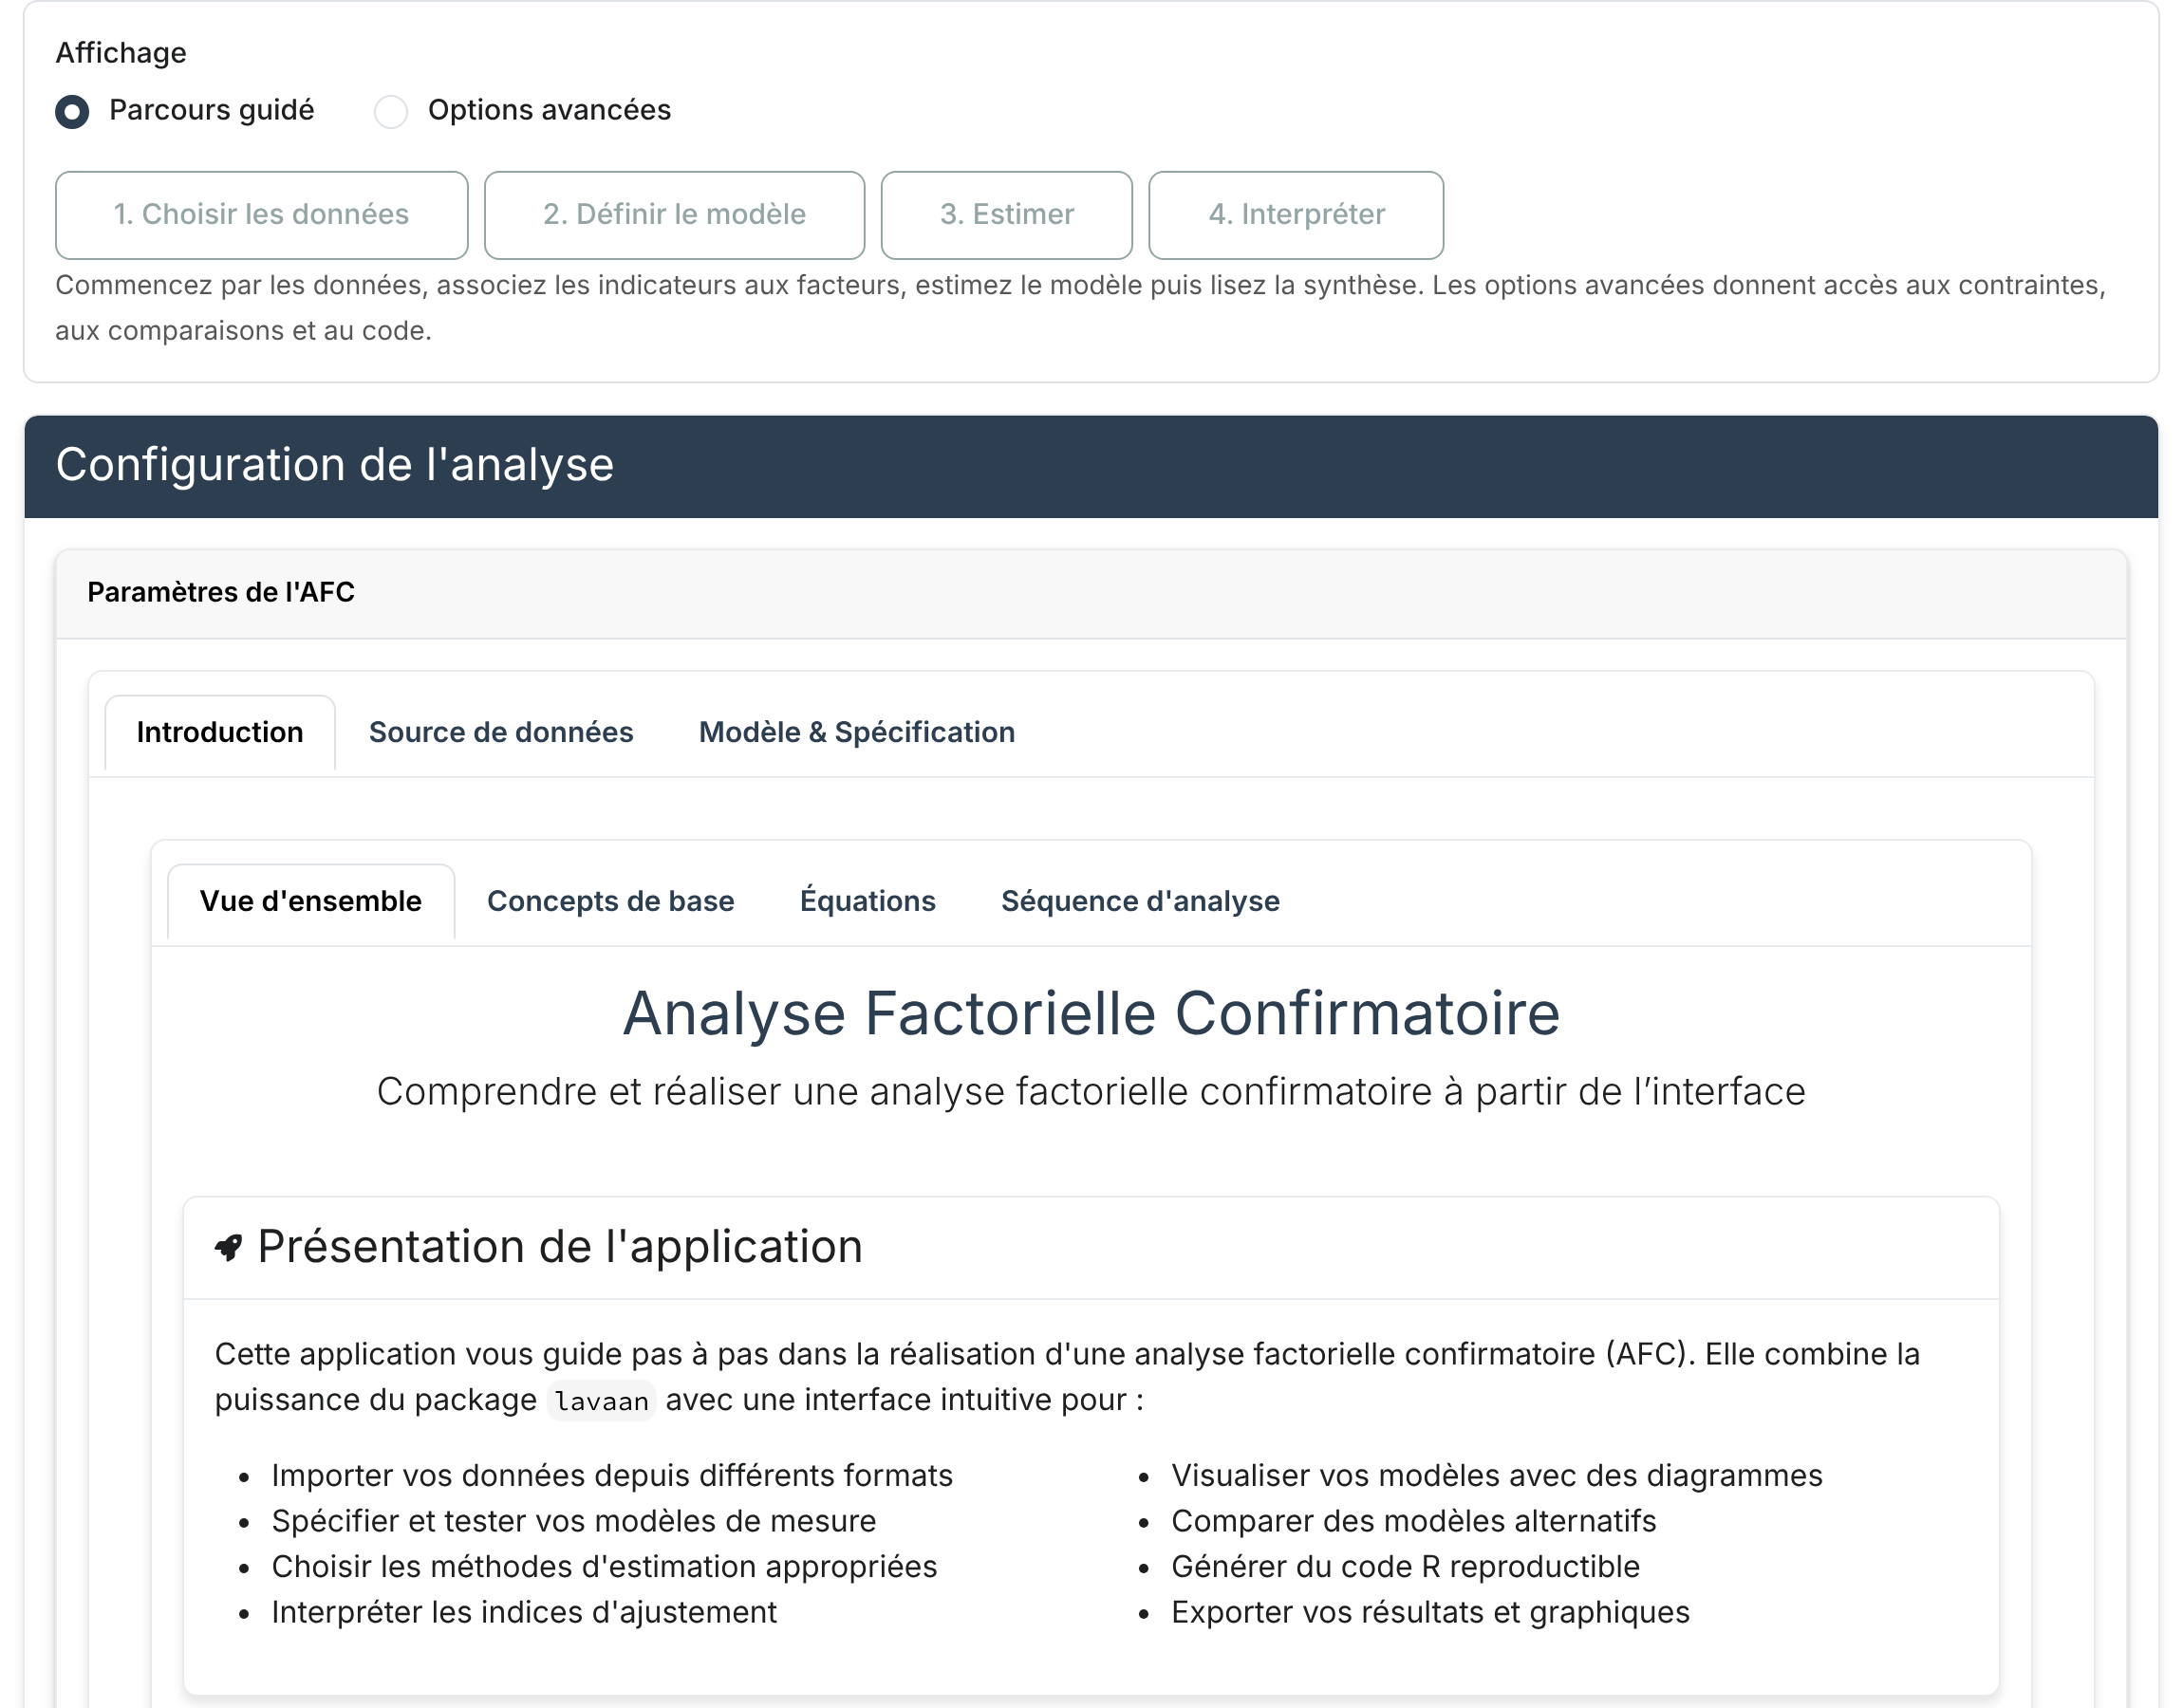
\includegraphics[width=1\linewidth,height=\textheight,keepaspectratio]{images/app/ch02_accueil.png}

}

\caption{\label{fig-app-accueil}Écran d'accueil. La barre des quatre
étapes et le choix du mode d'affichage restent visibles en permanence;
l'onglet \textbf{Introduction} rappelle les notions de base.}

\end{figure}%

\begin{figure}[htbp]

\centering{

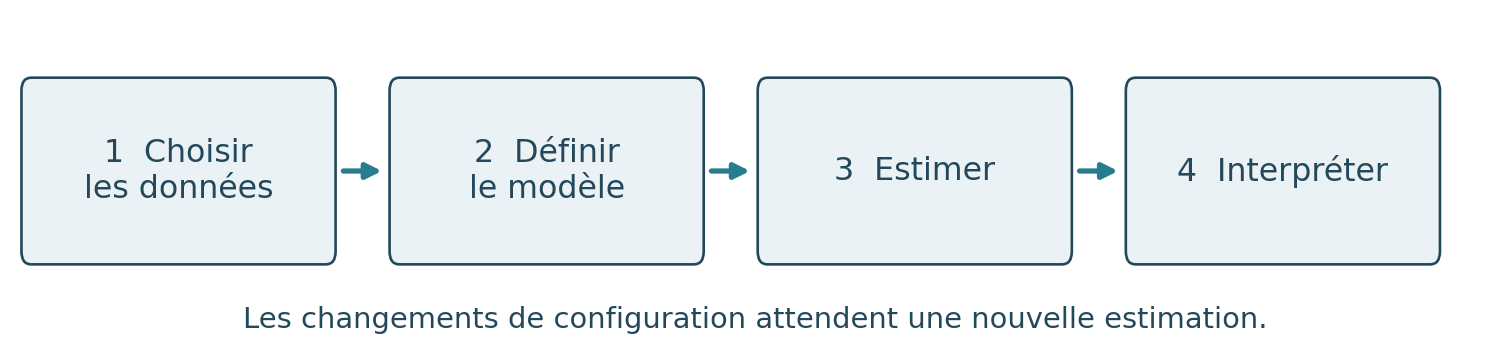
\includegraphics[width=1\linewidth,height=\textheight,keepaspectratio]{images/parcours.png}

}

\caption{\label{fig-parcours}Le parcours conserve une analyse estimée
jusqu'à la prochaine estimation; l'interprétation porte sur cette
analyse.}

\end{figure}%

\Needspace{8\baselineskip}

{\def\LTcaptype{none} % do not increment counter
\begin{longtable}[]{@{}
  >{\raggedright\arraybackslash}p{(\linewidth - 2\tabcolsep) * \real{0.5000}}
  >{\raggedright\arraybackslash}p{(\linewidth - 2\tabcolsep) * \real{0.5000}}@{}}
\toprule\noalign{}
\begin{minipage}[b]{\linewidth}\raggedright
Commande
\end{minipage} & \begin{minipage}[b]{\linewidth}\raggedright
Ce que vous y faites
\end{minipage} \\
\midrule\noalign{}
\endhead
\bottomrule\noalign{}
\endlastfoot
1. Choisir les données & Importer un fichier, sélectionner un exemple
réel ou préparer une simulation \\
2. Définir le modèle & Nommer les facteurs, associer les indicateurs et
vérifier les réglages \\
3. Estimer & Calculer et enregistrer l'analyse correspondant à cette
configuration \\
4. Interpréter & Lire la synthèse, les indices et les signaux de
l'analyse enregistrée \\
\end{longtable}
}

Le bouton \textbf{4. Interpréter} devient utile après une estimation
réussie. Il ouvre une vue dédiée; il ne lance pas une nouvelle
estimation. \textbf{Revenir aux résultats} ramène aux tableaux et
graphiques de la même analyse.

\section{Deux modes d'affichage}\label{deux-modes-daffichage}

\textbf{Parcours guidé} présente les commandes courantes.
\textbf{Options avancées} ajoute notamment les contraintes, les
comparaisons et le code. Commencez en parcours guidé. Les activités
avancées indiquent explicitement quand changer de mode.

Changer de mode ne supprime pas les restrictions déjà posées. Si des
contraintes restent actives, l'application les signale. Masquer un
panneau n'annule pas ses réglages. Pour repartir sans ancienne
contrainte, utilisez \textbf{Réinitialiser}, puis rechargez le modèle de
l'exemple.

\Needspace{10\baselineskip}

{\def\LTcaptype{none} % do not increment counter
\begin{longtable}[]{@{}
  >{\raggedright\arraybackslash}p{(\linewidth - 4\tabcolsep) * \real{0.2308}}
  >{\centering\arraybackslash}p{(\linewidth - 4\tabcolsep) * \real{0.3846}}
  >{\centering\arraybackslash}p{(\linewidth - 4\tabcolsep) * \real{0.3846}}@{}}
\toprule\noalign{}
\begin{minipage}[b]{\linewidth}\raggedright
Élément
\end{minipage} & \begin{minipage}[b]{\linewidth}\centering
Parcours guidé
\end{minipage} & \begin{minipage}[b]{\linewidth}\centering
Options avancées
\end{minipage} \\
\midrule\noalign{}
\endhead
\bottomrule\noalign{}
\endlastfoot
Données, modèle, estimation, interprétation & oui & oui \\
Statistiques descriptives, fiabilité, validité, scores, diagramme & oui
& oui \\
Onglet \textbf{Contraintes} (covariances résiduelles, paramètres fixes)
& non & oui \\
\textbf{Analyse → Comparaisons} (tests d'égalité) & non & oui \\
HTMT2 et intervalles bootstrap dans \textbf{4. Interpréter} & non &
oui \\
Onglet \textbf{Code} (R et ébauche Stata) & non & oui \\
\end{longtable}
}

\section{La source de données}\label{la-source-de-donnuxe9es}

Trois choix sont possibles. \textbf{Charger un fichier} accepte
notamment CSV, SAV, DTA et Excel. \textbf{Données réelles} donne accès
aux sept fichiers inclus. \textbf{Données simulées} prépare une
population pédagogique et génère un échantillon à partir des réglages
choisis.

Dans les données réelles, sélectionner un nom charge le fichier pour
consultation. Le bouton \textbf{Charger cet exemple et son modèle}
accomplit une action supplémentaire : il remplace la structure du modèle
et prépare les réglages proposés. Ne confondez pas la sélection du
fichier avec la préparation du modèle.

\begin{figure}[htbp]

\centering{

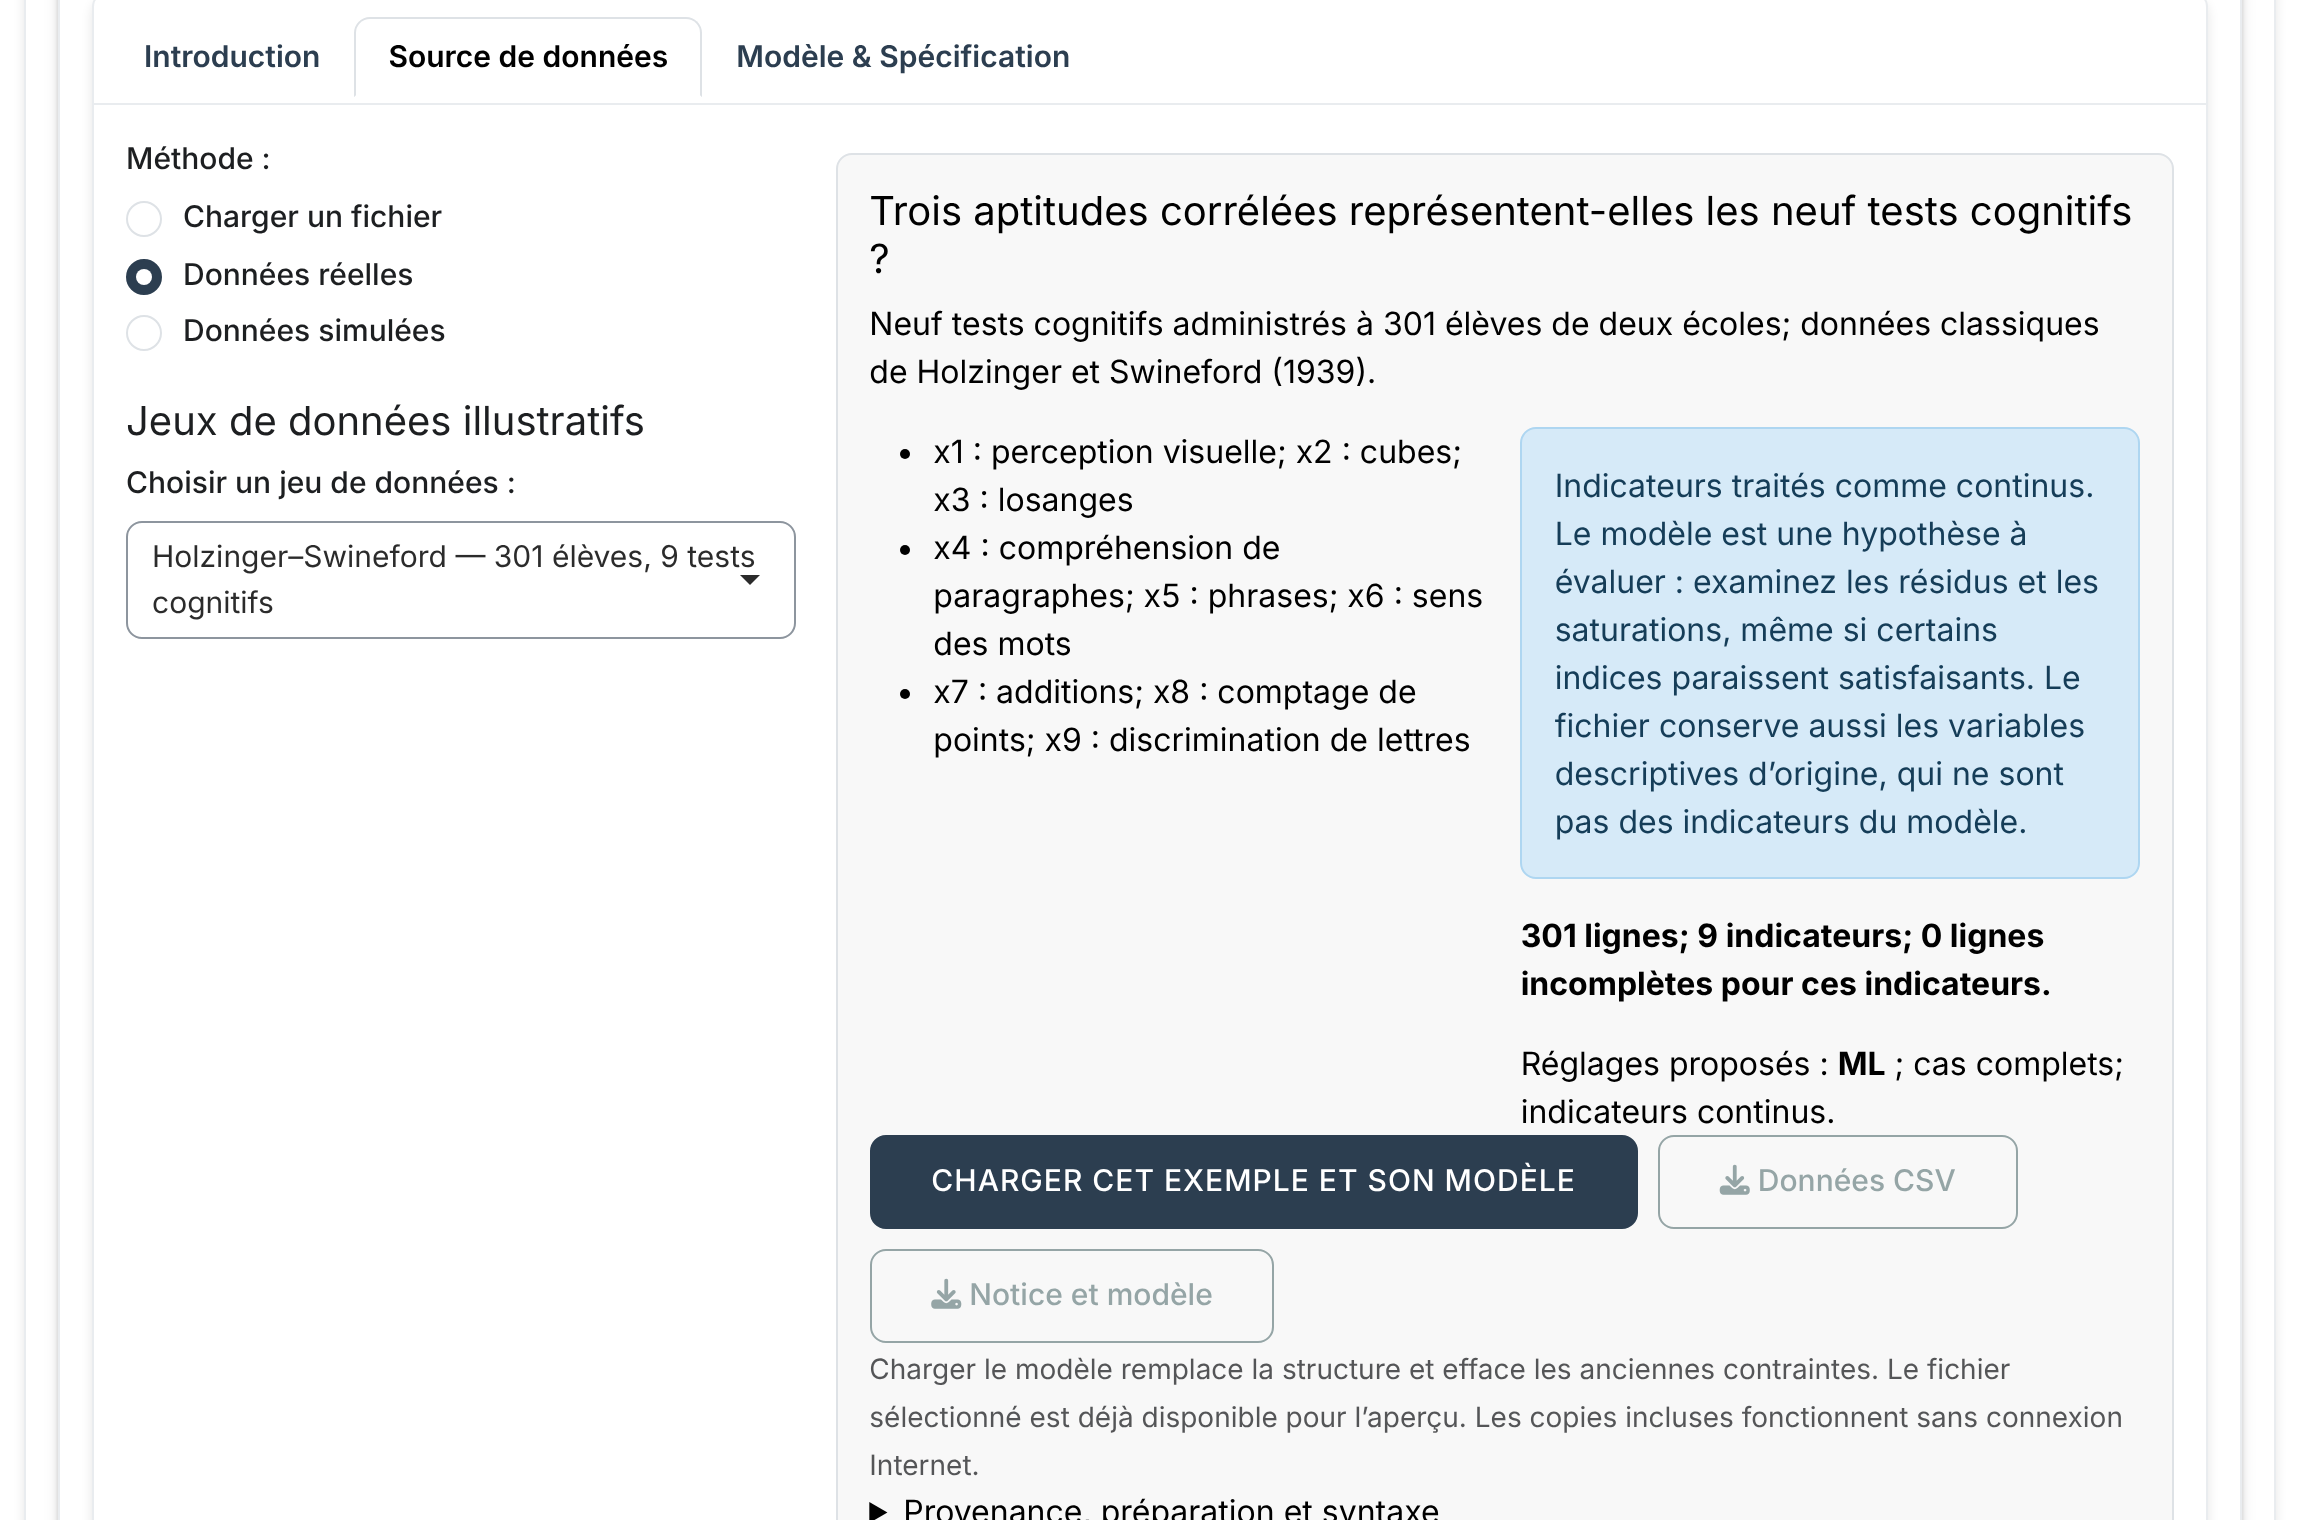
\includegraphics[width=1\linewidth,height=\textheight,keepaspectratio]{images/app/ch02_source.png}

}

\caption{\label{fig-app-source}\textbf{Source de données → Données
réelles}. La fiche de droite donne la question, le dictionnaire des
variables, une mise en garde, les effectifs et les réglages proposés. Le
bouton foncé prépare le modèle; les deux autres téléchargent le CSV et
la notice.}

\end{figure}%

Lisez la fiche avant de continuer. Elle précise la question, les
variables, leur codage, les lignes incomplètes et les limites de
l'exemple. Pour les jeux ordinaux, le chargement du modèle préconfigure
aussi les indicateurs ordinaux et WLSMV.

\section{La page Modèle et
Spécification}\label{la-page-moduxe8le-et-spuxe9cification}

La structure apparaît à gauche et l'estimation à droite sur une fenêtre
suffisamment large. Chaque facteur possède un nom et une sélection
d'indicateurs. Sur une fenêtre étroite, les blocs se placent l'un sous
l'autre; aucune étape n'est supprimée.

\begin{figure}[htbp]

\centering{

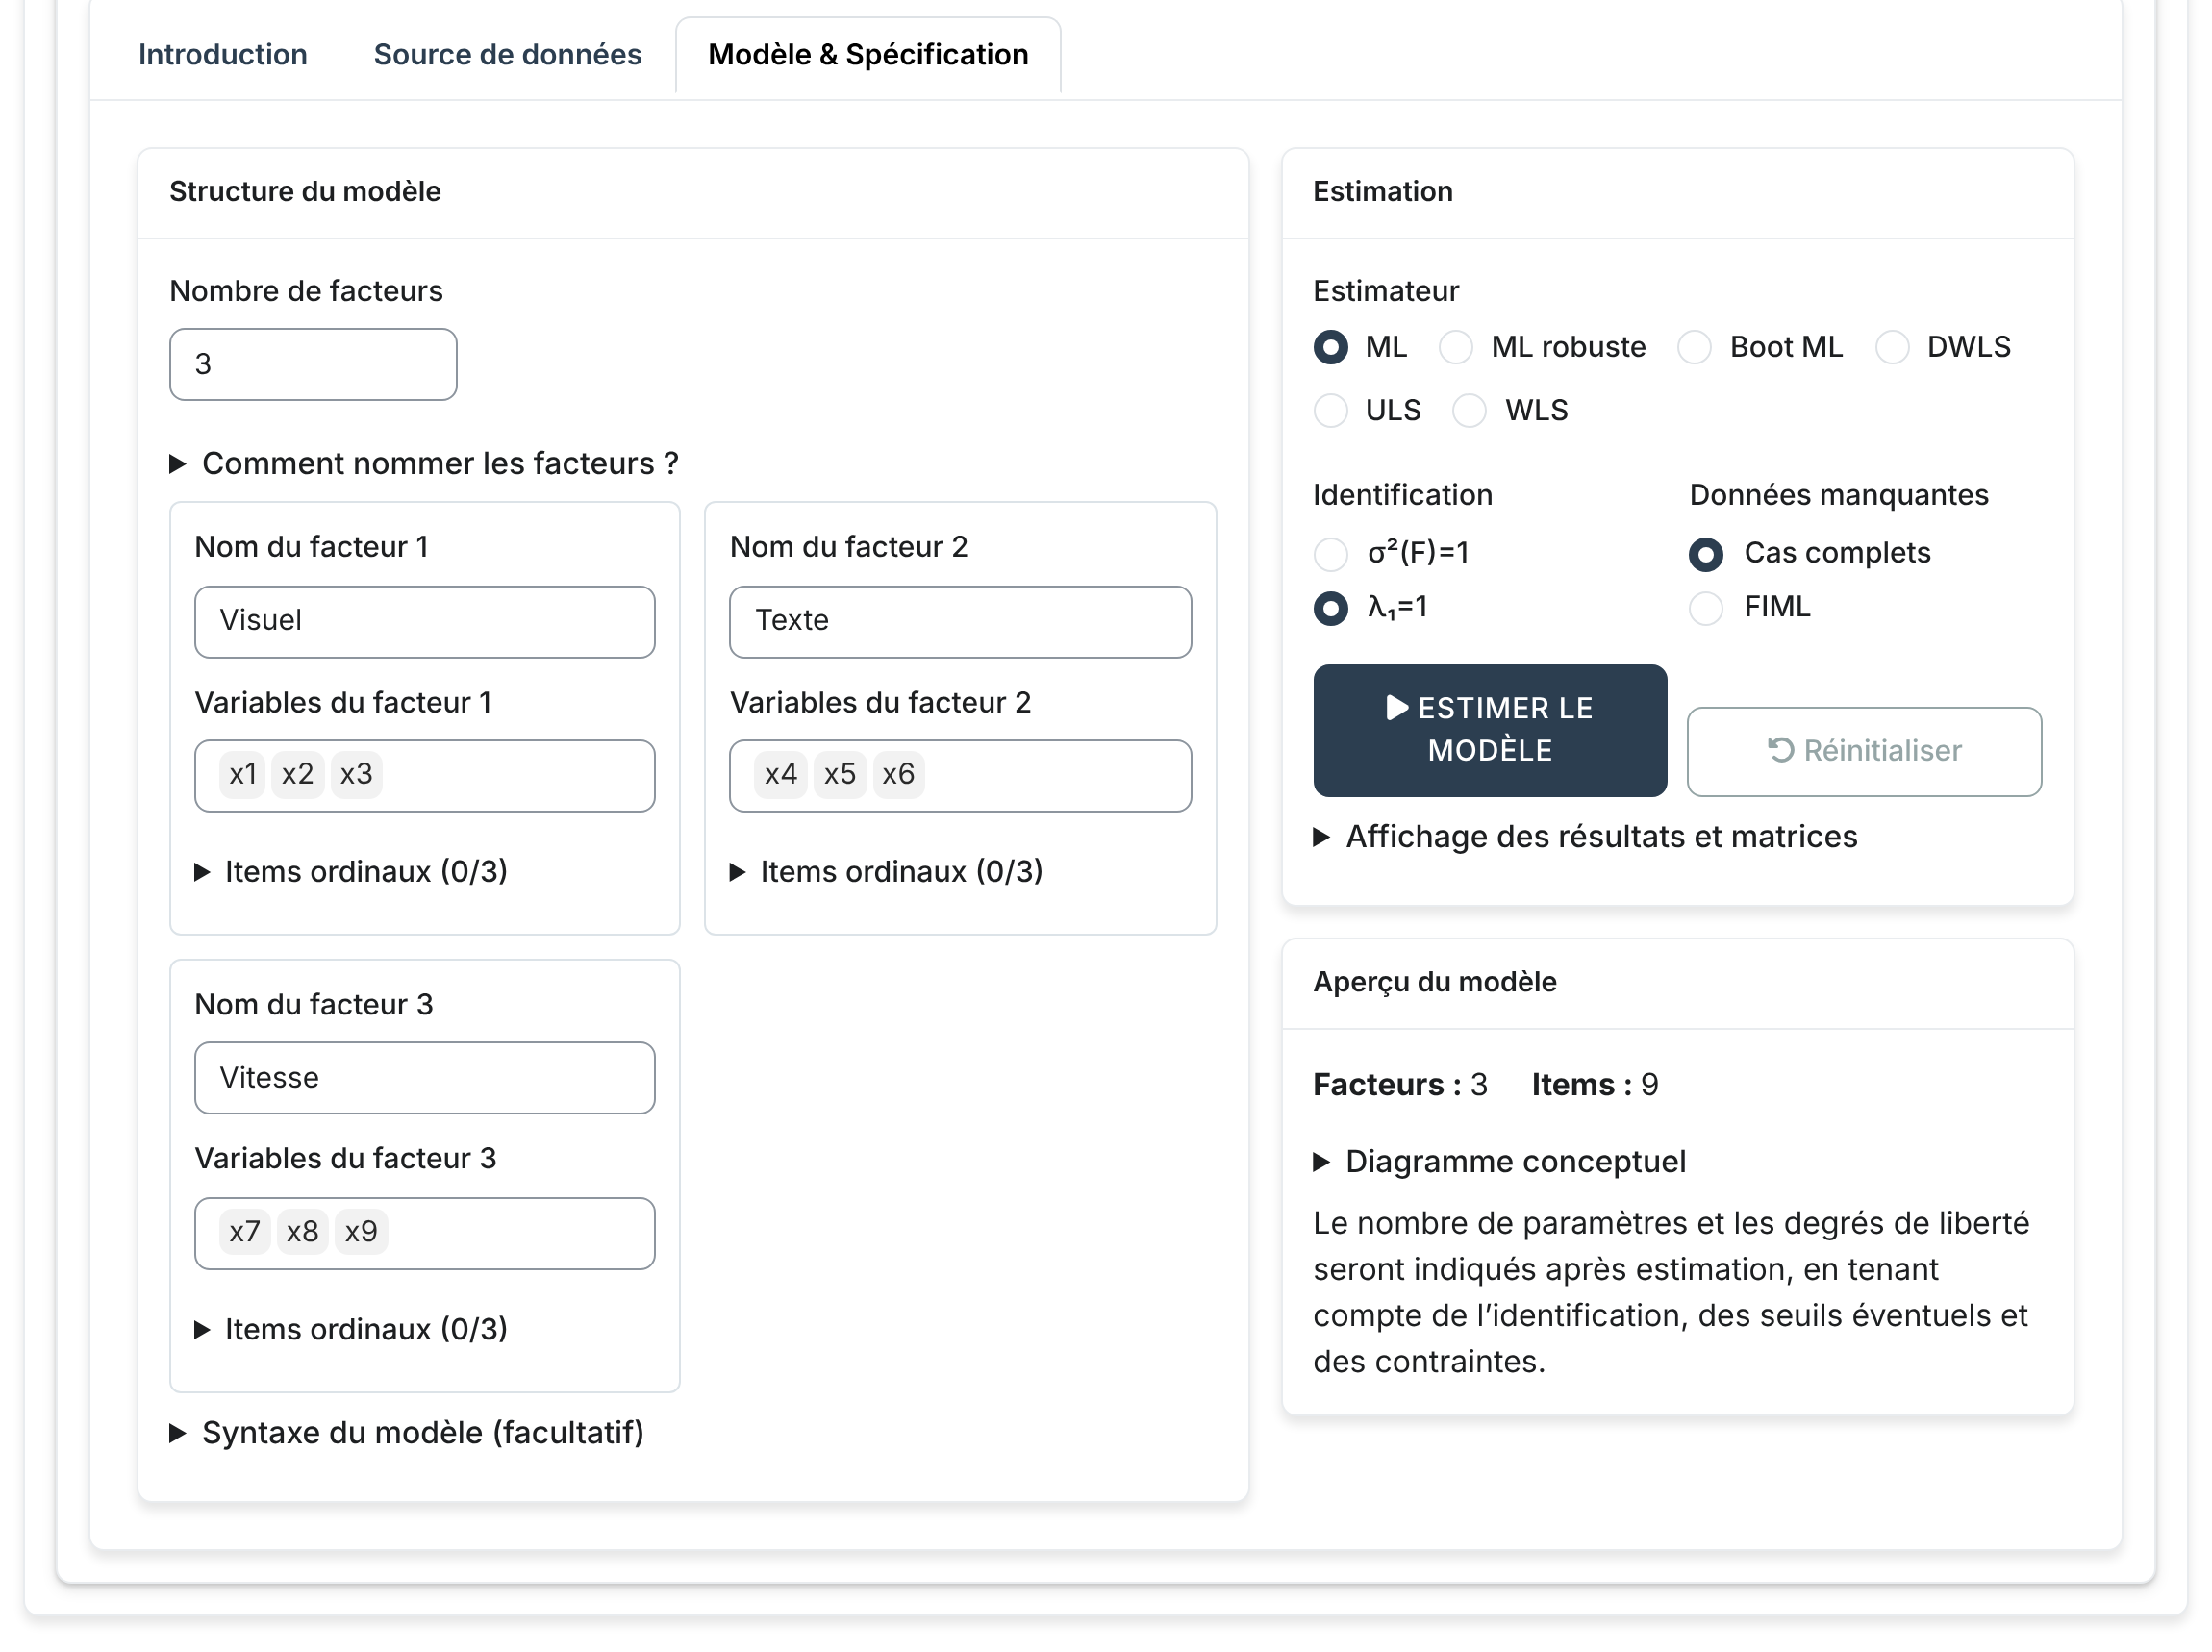
\includegraphics[width=1\linewidth,height=\textheight,keepaspectratio]{images/app/ch02_modele.png}

}

\caption{\label{fig-app-modele}\textbf{Modèle \& Spécification} après
\textbf{Charger cet exemple et son modèle} sur Holzinger--Swineford :
trois facteurs nommés, leurs indicateurs, puis l'estimateur,
l'identification et la gestion des données manquantes.}

\end{figure}%

Les noms doivent commencer par une lettre, être uniques et ne pas
reprendre le nom d'une colonne. Utilisez des lettres sans accent, des
chiffres ou un trait de soulignement : \texttt{Visuel},
\texttt{AffectPositif} ou \texttt{Engagement\_formation}. Le nom affiché
est un identifiant; vous pouvez employer un libellé plus développé dans
votre rapport.

Sous chaque facteur, \textbf{Items ordinaux} indique le nombre de
variables sélectionnées comme ordinales. Dépliez ce contrôle pour
vérifier ou modifier les cases. Une réponse binaire correcte/incorrecte
est aussi traitée comme catégorielle ordonnée dans les exemples
concernés.

Le \textbf{Diagramme conceptuel} montre la structure annoncée. Il ne
représente pas encore des estimations. Les options détaillées et la
syntaxe sont repliables pour garder les commandes principales
accessibles. Aucun code n'est nécessaire pour les manipulations de ce
manuel.

\section{Des résultats conservés après
estimation}\label{des-ruxe9sultats-conservuxe9s-apruxe8s-estimation}

Après une estimation réussie, les résultats s'ouvrent sur
\textbf{Données}. Les autres panneaux présentent les descriptives,
l'analyse, le diagramme et l'aide. Le bandeau indique notamment
l'effectif utilisé et les paramètres libres.

\begin{figure}[htbp]

\centering{

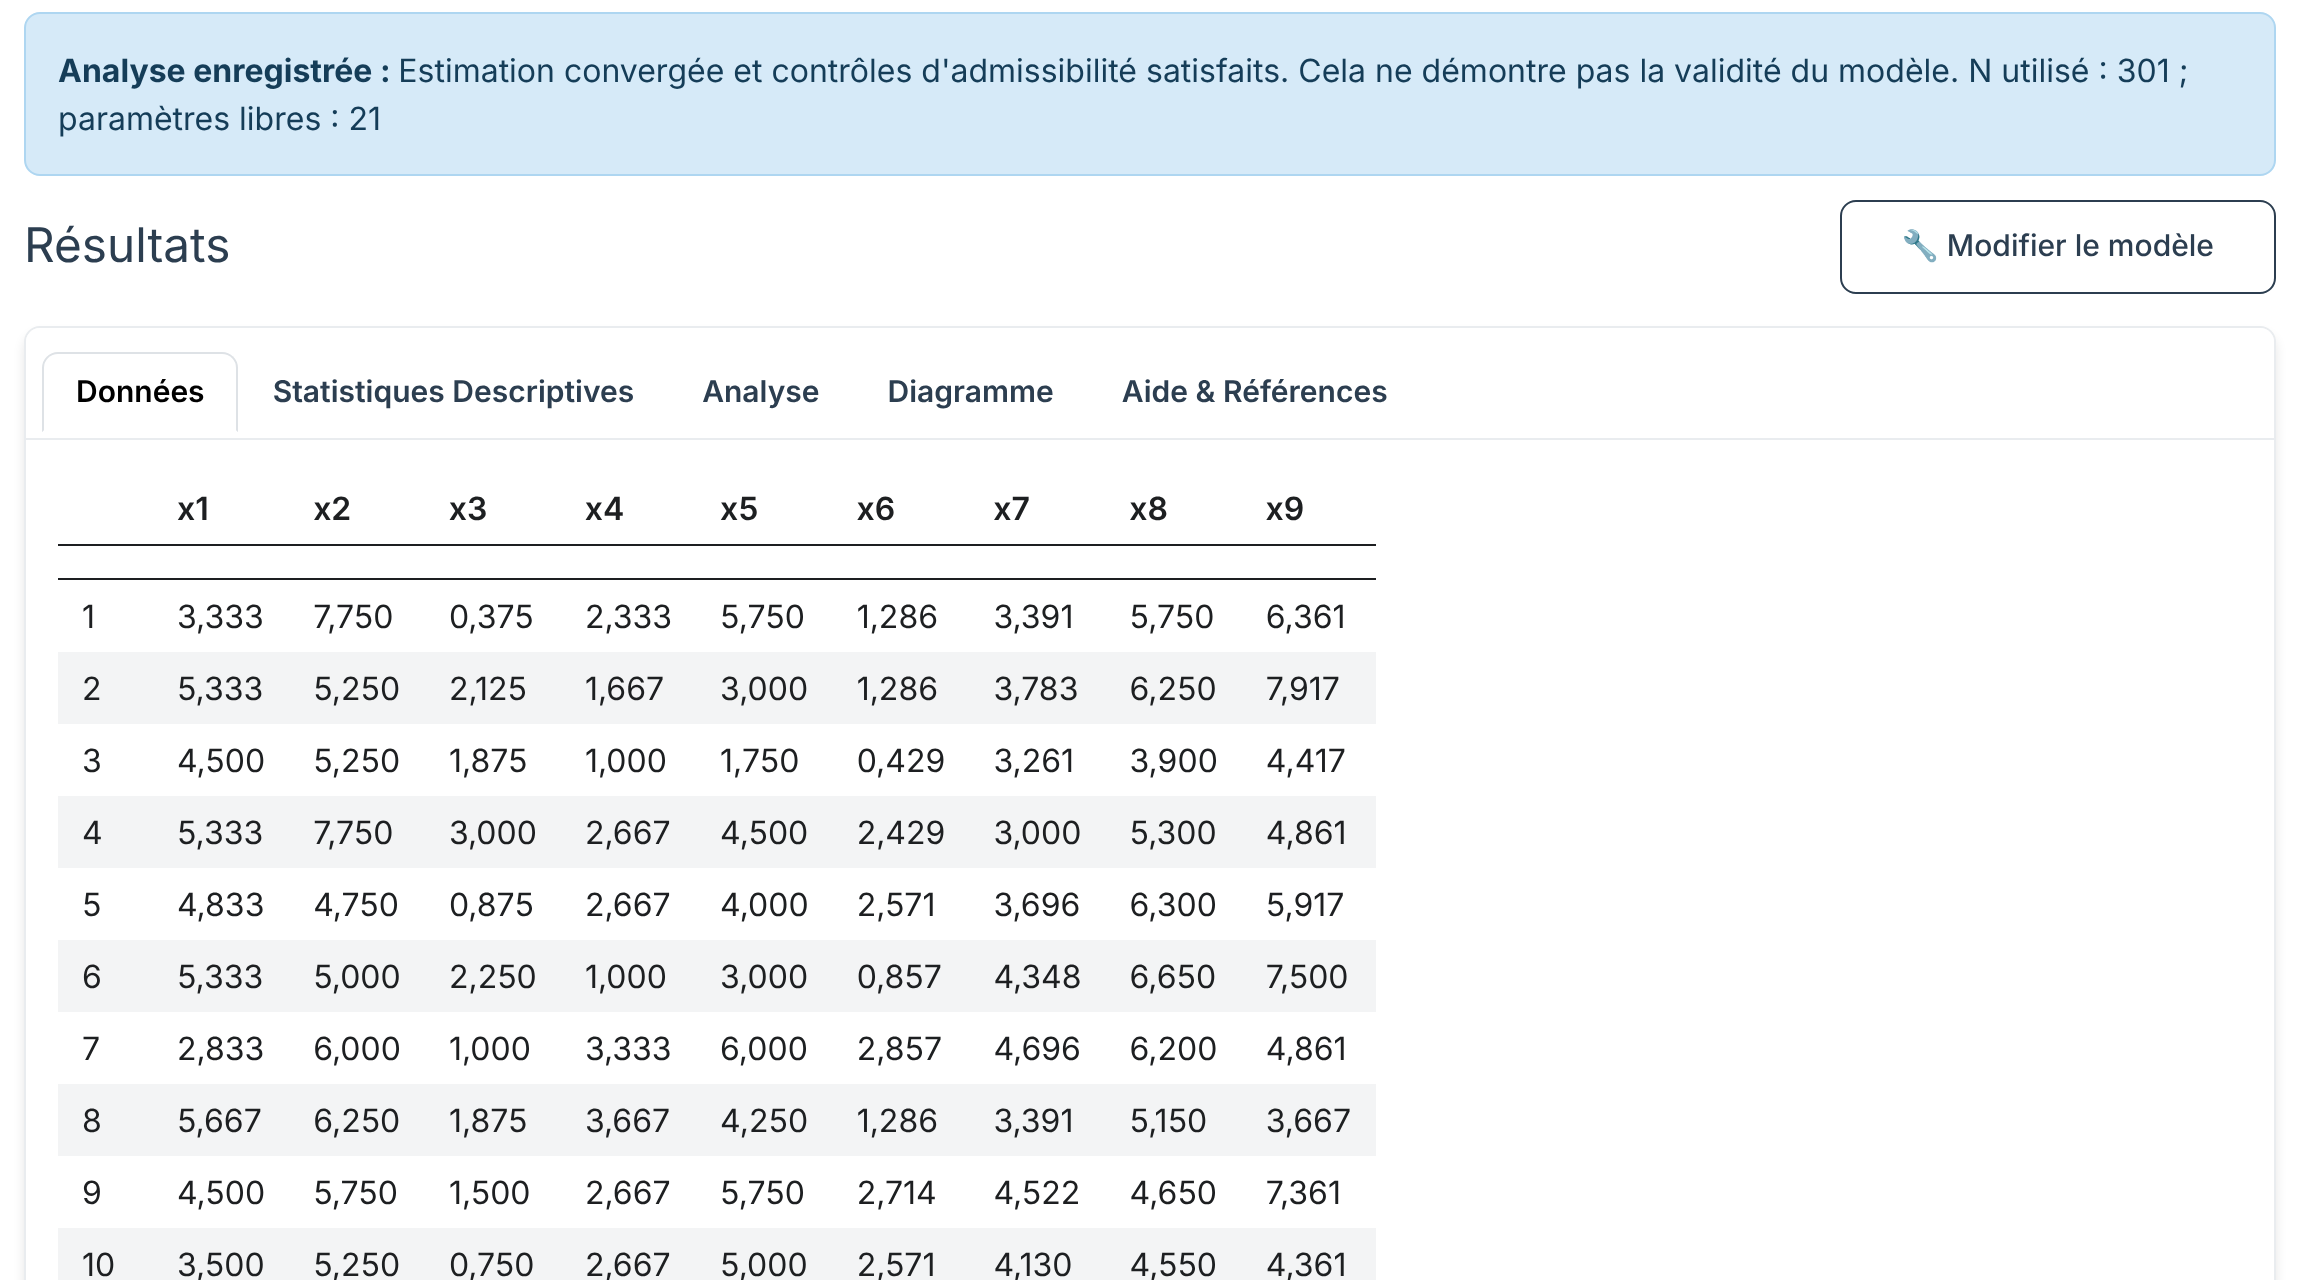
\includegraphics[width=1\linewidth,height=\textheight,keepaspectratio]{images/app/ch02_resultats.png}

}

\caption{\label{fig-app-resultats}Après \textbf{3. Estimer} : le bandeau
« Analyse enregistrée » annonce 301 observations utilisées et 21
paramètres libres. Les onglets de résultats portent tous sur cette
analyse.}

\end{figure}%

Si vous modifiez ensuite le modèle ou un réglage d'estimation, le
bandeau devient orange et rappelle que les résultats et exports
correspondent encore à l'analyse précédente. Ce comportement protège la
cohérence des documents téléchargés. Pour appliquer les changements,
cliquez de nouveau sur \textbf{3. Estimer}.

\begin{tcolorbox}[enhanced jigsaw, arc=.35mm, bottomrule=.15mm, bottomtitle=1mm, breakable, colback=white, colbacktitle=quarto-callout-warning-color!10!white, colframe=quarto-callout-warning-color-frame, coltitle=black, left=2mm, leftrule=.75mm, opacityback=0, opacitybacktitle=0.6, rightrule=.15mm, title={Avant de recopier un résultat}, titlerule=0mm, toprule=.15mm, toptitle=1mm]

Vérifiez le nom du fichier, les indicateurs, l'estimateur et l'effectif
de l'analyse enregistrée. Un changement visible dans les contrôles n'est
pas nécessairement un changement déjà appliqué aux résultats.

\end{tcolorbox}

\section{Réinitialiser sans perdre le
fichier}\label{ruxe9initialiser-sans-perdre-le-fichier}

\textbf{Réinitialiser} efface les anciennes contraintes, les covariances
résiduelles ajoutées, les comparaisons et les résultats disponibles. Les
données restent chargées. Vous devrez redéfinir ou recharger la
structure à analyser. Ce bouton ne remplace pas le téléchargement
préalable d'un rapport que vous souhaitez conserver.

Pour reprendre un exemple à son point de départ, la procédure la plus
simple est : retourner à \textbf{Données réelles}, sélectionner le jeu
et cliquer sur \textbf{Charger cet exemple et son modèle}. Relisez
ensuite les réglages avant d'estimer.

\section{Laboratoire : préparer une analyse sans
l'estimer}\label{laboratoire-pruxe9parer-une-analyse-sans-lestimer}

\begin{enumerate}
\def\labelenumi{\arabic{enumi}.}
\tightlist
\item
  Ouvrez \textbf{1. Choisir les données}, puis \textbf{Données réelles}.
\item
  Sélectionnez Holzinger--Swineford et lisez la fiche.
\item
  Téléchargez la \textbf{Notice et modèle} et les \textbf{Données CSV}.
\item
  Cliquez sur \textbf{Charger cet exemple et son modèle}.
\item
  Vérifiez que trois facteurs apparaissent et que leurs noms sont
  \texttt{Visuel}, \texttt{Texte} et \texttt{Vitesse}.
\item
  Dépliez le \textbf{Diagramme conceptuel} et retrouvez les trois
  groupes d'indicateurs.
\end{enumerate}

Questions : combien de lignes et d'indicateurs la fiche annonce-t-elle ?
Quel estimateur est proposé ? Le diagramme affiche-t-il des coefficients
?

\begin{tcolorbox}[enhanced jigsaw, arc=.35mm, bottomrule=.15mm, bottomtitle=1mm, breakable, colback=white, colbacktitle=quarto-callout-tip-color!10!white, colframe=quarto-callout-tip-color-frame, coltitle=black, left=2mm, leftrule=.75mm, opacityback=0, opacitybacktitle=0.6, rightrule=.15mm, title={Réponse}, titlerule=0mm, toprule=.15mm, toptitle=1mm]

La fiche annonce 301 lignes, 9 indicateurs et aucune ligne incomplète
pour ces indicateurs. L'estimateur proposé est ML, avec les cas complets
et des indicateurs continus. Le diagramme conceptuel n'affiche aucun
coefficient : il représente la structure annoncée, pas une estimation.
Vous avez préparé une analyse; vous n'avez encore ni estimé les
paramètres ni évalué l'ajustement.

\end{tcolorbox}

\begin{tcolorbox}[enhanced jigsaw, arc=.35mm, bottomrule=.15mm, bottomtitle=1mm, breakable, colback=white, colbacktitle=quarto-callout-important-color!10!white, colframe=quarto-callout-important-color-frame, coltitle=black, left=2mm, leftrule=.75mm, opacityback=0, opacitybacktitle=0.6, rightrule=.15mm, title={À retenir}, titlerule=0mm, toprule=.15mm, toptitle=1mm]

\begin{itemize}
\tightlist
\item
  Les quatre étapes vont des données à l'interprétation; seule
  \textbf{3. Estimer} produit une nouvelle analyse.
\item
  \textbf{Charger cet exemple et son modèle} remplace la structure et
  les réglages; sélectionner un jeu ne fait que l'ouvrir.
\item
  Un bandeau orange signale que les contrôles ne correspondent plus aux
  résultats affichés.
\item
  \textbf{Réinitialiser} efface contraintes et résultats, pas les
  données.
\end{itemize}

\end{tcolorbox}

\section{Quiz}\label{quiz-1}

\begin{enumerate}
\def\labelenumi{\arabic{enumi}.}
\tightlist
\item
  Vous changez l'estimateur après une estimation, puis téléchargez le
  rapport. Quelle analyse le rapport décrit-il ?
\item
  Le bouton \textbf{4. Interpréter} lance-t-il une estimation ?
\item
  Où se trouvent les tests d'égalité de saturations ?
\item
  Vous passez du mode avancé au mode guidé. Une covariance résiduelle
  ajoutée est-elle supprimée ?
\end{enumerate}

\begin{tcolorbox}[enhanced jigsaw, arc=.35mm, bottomrule=.15mm, bottomtitle=1mm, breakable, colback=white, colbacktitle=quarto-callout-tip-color!10!white, colframe=quarto-callout-tip-color-frame, coltitle=black, left=2mm, leftrule=.75mm, opacityback=0, opacitybacktitle=0.6, rightrule=.15mm, title={Réponses}, titlerule=0mm, toprule=.15mm, toptitle=1mm]

\begin{enumerate}
\def\labelenumi{\arabic{enumi}.}
\tightlist
\item
  L'analyse estimée précédemment : le changement d'estimateur ne
  s'applique qu'après \textbf{3. Estimer}.
\item
  Non. Il ouvre la synthèse de l'analyse enregistrée.
\item
  Dans \textbf{Analyse → Comparaisons}, visible en \textbf{Options
  avancées}.
\item
  Non. Masquer un panneau n'annule pas ses réglages; l'application
  signale les contraintes encore actives.
\end{enumerate}

\end{tcolorbox}

\bookmarksetup{startatroot}

\chapter{Réaliser sa première AFC de bout en bout}\label{sec-premiere}

\begin{tcolorbox}[enhanced jigsaw, arc=.35mm, bottomrule=.15mm, bottomtitle=1mm, breakable, colback=white, colbacktitle=quarto-callout-note-color!10!white, colframe=quarto-callout-note-color-frame, coltitle=black, left=2mm, leftrule=.75mm, opacityback=0, opacitybacktitle=0.6, rightrule=.15mm, title={Objectifs du chapitre}, titlerule=0mm, toprule=.15mm, toptitle=1mm]

\begin{itemize}
\tightlist
\item
  Préparer, estimer et vérifier un modèle à trois facteurs corrélés.
\item
  Lire les saturations non standardisées et standardisées.
\item
  Interpréter les corrélations entre facteurs sans leur prêter un sens
  causal.
\item
  Conserver l'analyse dans un rapport avant toute modification.
\end{itemize}

\end{tcolorbox}

\begin{tcolorbox}[enhanced jigsaw, arc=.35mm, bottomrule=.15mm, bottomtitle=1mm, breakable, colback=white, colbacktitle=quarto-callout-tip-color!10!white, colframe=quarto-callout-tip-color-frame, coltitle=black, left=2mm, leftrule=.75mm, opacityback=0, opacitybacktitle=0.6, rightrule=.15mm, title={Idée centrale}, titlerule=0mm, toprule=.15mm, toptitle=1mm]

Avant d'interpréter, on vérifie que l'analyse est bien celle qu'on
voulait : bon fichier, bons indicateurs, bon estimateur, effectif
attendu, solution admissible. Ensuite seulement, on lit les saturations
standardisées, puis les relations entre facteurs.

\end{tcolorbox}

\section{La question et les
données}\label{la-question-et-les-donnuxe9es}

Nous examinons neuf tests cognitifs de 301 élèves, regroupés dans le
fichier Holzinger--Swineford. L'hypothèse de départ distingue trois
aptitudes corrélées : une dimension visuelle, une dimension verbale et
une dimension de vitesse. Cette structure est couramment utilisée pour
illustrer l'AFC; son caractère classique ne garantit pas qu'elle décrive
parfaitement les données (\citeproc{ref-lavaancfa}{Projet lavaan
2026a}).

Dans ce premier exercice, les neuf résultats sont traités comme
continus. Les variables descriptives supplémentaires du fichier, dont
l'école, ne sont pas utilisées comme indicateurs. L'analyse porte sur
l'ensemble des élèves, sans analyse multigroupe.

\section{Préparer exactement le
modèle}\label{pruxe9parer-exactement-le-moduxe8le}

\begin{enumerate}
\def\labelenumi{\arabic{enumi}.}
\tightlist
\item
  Dans \textbf{1. Choisir les données}, cochez \textbf{Données réelles}.
\item
  Sélectionnez \textbf{Holzinger--Swineford} et lisez la fiche.
\item
  Cliquez sur \textbf{Charger cet exemple et son modèle}.
\item
  Dans \textbf{Modèle \& Spécification}, vérifiez les associations du
  tableau ci-dessous.
\end{enumerate}

\Needspace{7\baselineskip}

{\def\LTcaptype{none} % do not increment counter
\begin{longtable}[]{@{}
  >{\raggedright\arraybackslash}p{(\linewidth - 4\tabcolsep) * \real{0.3333}}
  >{\raggedright\arraybackslash}p{(\linewidth - 4\tabcolsep) * \real{0.3333}}
  >{\raggedright\arraybackslash}p{(\linewidth - 4\tabcolsep) * \real{0.3333}}@{}}
\toprule\noalign{}
\begin{minipage}[b]{\linewidth}\raggedright
Facteur
\end{minipage} & \begin{minipage}[b]{\linewidth}\raggedright
Indicateurs à sélectionner
\end{minipage} & \begin{minipage}[b]{\linewidth}\raggedright
Sens général
\end{minipage} \\
\midrule\noalign{}
\endhead
\bottomrule\noalign{}
\endlastfoot
Visuel & \texttt{x1}, \texttt{x2}, \texttt{x3} & Perception visuelle,
cubes, losanges \\
Texte & \texttt{x4}, \texttt{x5}, \texttt{x6} & Compréhension, phrases,
sens des mots \\
Vitesse & \texttt{x7}, \texttt{x8}, \texttt{x9} & Additions, comptage de
points, discrimination de lettres \\
\end{longtable}
}

Ne sélectionnez pas les neuf variables pour chacun des facteurs. Chaque
indicateur appartient ici à un seul groupe. Aucune covariance résiduelle
n'est ajoutée.

Vérifiez ensuite \textbf{ML}, \textbf{λ₁=1} et \textbf{Cas complets}.
Les contrôles \textbf{Items ordinaux} doivent être à zéro pour cet
exercice. Dans \textbf{Affichage des résultats et matrices}, conservez
\textbf{Coeff. Std.}, et cochez également \textbf{R²} et
\textbf{Ajustement}. Ne cochez pas \textbf{Moyennes} pour cette première
comparaison de covariances.

Cliquez sur \textbf{3. Estimer}, ou sur \textbf{Estimer le modèle} dans
le panneau de configuration. Les deux commandes déclenchent l'analyse.
Si une erreur apparaît, ne poursuivez pas vers l'interprétation :
comparez vos sélections et réglages à cette liste.

\section{Vérifier avant
d'interpréter}\label{vuxe9rifier-avant-dinterpruxe9ter}

Le bandeau de l'analyse doit annoncer une estimation convergée et
admissible. Vous devez retrouver \textbf{301 observations utilisées} et
\textbf{21 paramètres libres}. Dans cette configuration, le modèle
comporte \textbf{24 degrés de liberté}. Ces informations constituent des
contrôles de cohérence, pas une preuve de validité.

Dans \textbf{Données}, vérifiez les noms des indicateurs. Puis ouvrez
\textbf{Statistiques Descriptives → Univariées} et repérez les échelles
différentes des tests. Des unités différentes justifient de distinguer
coefficients non standardisés et standardisés.

\Needspace{13\baselineskip}

{

\begin{longtable}[]{@{}lrrrr@{}}

\caption{\label{tbl-hs-desc}Statistiques descriptives des neuf tests
(301 élèves). Les moyennes et les étendues diffèrent d'un test à l'autre
: les saturations non standardisées ne sont donc pas directement
comparables.}

\tabularnewline

\toprule\noalign{}
Item & Moyenne & ET & Min & Max \\
\midrule\noalign{}
\endhead
\bottomrule\noalign{}
\endlastfoot
x1 & 4,94 & 1,17 & 0,67 & 8,50 \\
x2 & 6,09 & 1,18 & 2,25 & 9,25 \\
x3 & 2,25 & 1,13 & 0,25 & 4,50 \\
x4 & 3,06 & 1,16 & 0,00 & 6,33 \\
x5 & 4,34 & 1,29 & 1,00 & 7,00 \\
x6 & 2,19 & 1,10 & 0,14 & 6,14 \\
x7 & 4,19 & 1,09 & 1,30 & 7,43 \\
x8 & 5,53 & 1,01 & 3,05 & 10,00 \\
x9 & 5,37 & 1,01 & 2,78 & 9,25 \\

\end{longtable}

}

\section{Lire les paramètres}\label{lire-les-paramuxe8tres}

Ouvrez \textbf{Analyse → Analyse de base → Résultats}. La sortie emploie
des termes anglais issus du moteur de calcul. Les principales colonnes
ont le sens suivant :

\Needspace{9\baselineskip}

{\def\LTcaptype{none} % do not increment counter
\begin{longtable}[]{@{}ll@{}}
\toprule\noalign{}
Colonne & Lecture \\
\midrule\noalign{}
\endhead
\bottomrule\noalign{}
\endlastfoot
Estimate & Coefficient dans l'échelle non standardisée \\
Std.Err & Erreur-type de l'estimation libre \\
z-value et P(\textgreater\textbar z\textbar) & Test du coefficient libre
contre zéro \\
Std.lv & Standardisation des variables latentes \\
Std.all & Standardisation des facteurs et des indicateurs \\
\end{longtable}
}

\begin{figure}[htbp]

\centering{

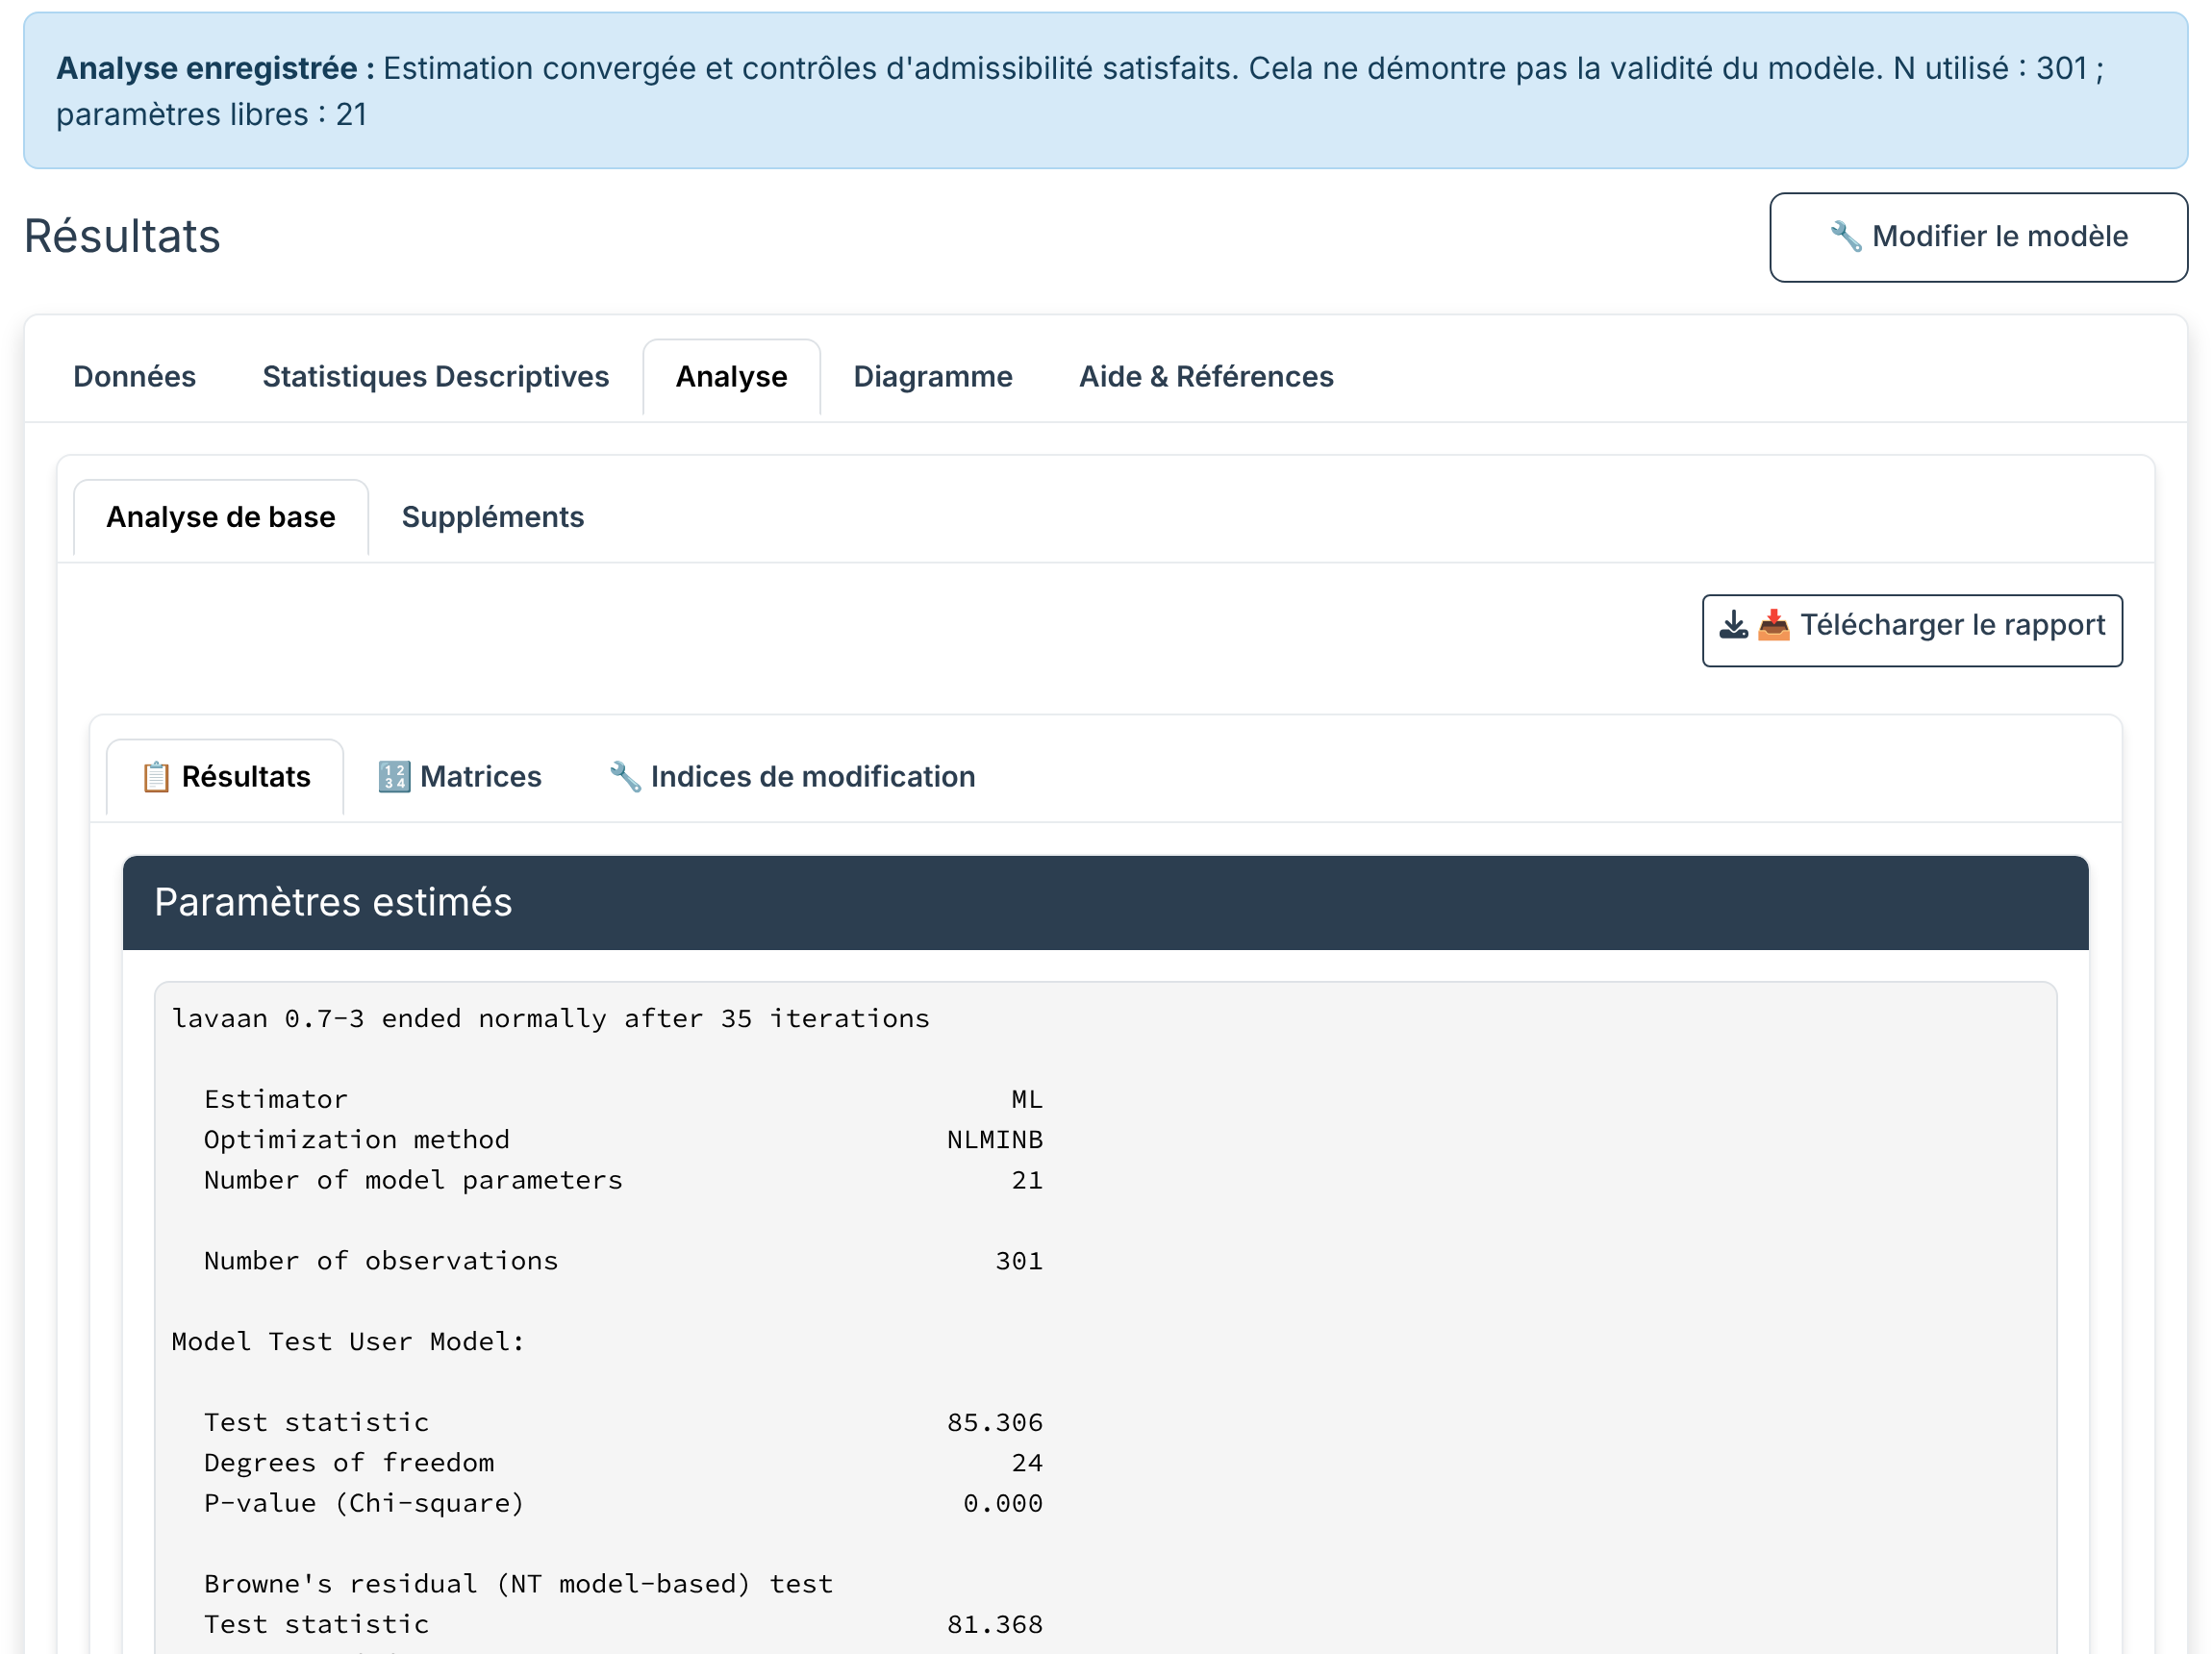
\includegraphics[width=1\linewidth,height=\textheight,keepaspectratio]{images/app/ch03_parametres.png}

}

\caption{\label{fig-app-parametres}\textbf{Analyse → Analyse de base →
Résultats}. La sortie détaillée commence par l'estimateur, le nombre de
paramètres et d'observations, puis le test du modèle. Les relations de
mesure (\texttt{=\textasciitilde{}}) suivent plus bas.}

\end{figure}%

Dans les relations de mesure, la notation \texttt{=\textasciitilde{}}
indique qu'un facteur est mesuré par des indicateurs. Le coefficient non
standardisé de \texttt{x1}, \texttt{x4} et \texttt{x7} est fixé à 1,
puisqu'ils servent de références. Leur valeur 1 ne signifie pas que ces
tests mesurent parfaitement leur facteur.

Les saturations \textbf{Std.all} sont les repères les plus simples pour
commencer :

\Needspace{13\baselineskip}

{

\begin{longtable}[]{@{}llrr@{}}

\caption{\label{tbl-hs-sat}Saturations entièrement standardisées
(Std.all) du modèle à trois facteurs et part de variance expliquée de
chaque test (carré de la saturation).}

\tabularnewline

\toprule\noalign{}
Facteur & Item & Saturation & Variance expliquée \\
\midrule\noalign{}
\endhead
\bottomrule\noalign{}
\endlastfoot
Visuel & x1 & 0,772 & 0,596 \\
Visuel & x2 & 0,424 & 0,179 \\
Visuel & x3 & 0,581 & 0,338 \\
Texte & x4 & 0,852 & 0,725 \\
Texte & x5 & 0,855 & 0,731 \\
Texte & x6 & 0,838 & 0,702 \\
Vitesse & x7 & 0,570 & 0,324 \\
Vitesse & x8 & 0,723 & 0,523 \\
Vitesse & x9 & 0,665 & 0,442 \\

\end{longtable}

}

\begin{figure}[htbp]

\centering{

\includegraphics[width=0.88\linewidth,height=\textheight,keepaspectratio]{03-premiere-afc_files/figure-pdf/fig-hs-sat-1.png}

}

\caption{\label{fig-hs-sat}Saturations standardisées du modèle de
référence. La ligne pointillée marque le repère descriptif de 0,40
utilisé par les signaux de l'application; x2 le dépasse de peu.}

\end{figure}%

\texttt{x2} est moins fortement lié au facteur visuel que \texttt{x1}.
Cette différence invite à examiner le contenu et l'incertitude de
mesure. Elle ne conduit pas automatiquement à supprimer \texttt{x2}. Les
trois tests verbaux ont ici des saturations standardisées élevées.

Pour un indicateur associé à un seul facteur, le carré de sa saturation
standardisée donne la proportion de variance expliquée dans ce modèle.
Avec une saturation de 0,424, on obtient \(0{,}424^2=0{,}179\). Le
facteur visuel explique donc environ 18~\% de la variance de
\texttt{x2}, sous cette spécification. C'est la valeur que l'application
affiche dans la section \textbf{R-Square} lorsque \textbf{R²} est coché.

\section{Lire les relations entre
facteurs}\label{lire-les-relations-entre-facteurs}

Les facteurs sont autorisés à covarier. Les corrélations estimées sont :

\Needspace{7\baselineskip}

{

\begin{longtable}[]{@{}lr@{}}

\caption{\label{tbl-hs-cor}Corrélations entre facteurs estimées par le
modèle de référence.}

\tabularnewline

\toprule\noalign{}
Paire & Corrélation \\
\midrule\noalign{}
\endhead
\bottomrule\noalign{}
\endlastfoot
Visuel -- Texte & 0,459 \\
Visuel -- Vitesse & 0,471 \\
Texte -- Vitesse & 0,283 \\

\end{longtable}

}

Les facteurs visuel et verbal sont liés (0,459), mais le modèle ne les
impose pas identiques. La relation la plus faible unit le texte et la
vitesse (0,283). Une corrélation factorielle ne démontre pas une
relation causale. Ces liens sont estimés à partir des relations entre
indicateurs, sous les hypothèses du modèle. Ils sont plus élevés que les
corrélations entre les tests eux-mêmes, car le modèle corrige
l'atténuation due à l'erreur de mesure.

\section{Porter un premier jugement sur
l'ensemble}\label{porter-un-premier-jugement-sur-lensemble}

Cliquez sur \textbf{4. Interpréter}. Lisez séparément le constat
numérique, les indices d'ajustement et les signaux à examiner. Le modèle
converge, mais les données ne sont pas reproduites sans écart : le CFI
vaut 0,931 et le RMSEA 0,092. Le chapitre suivant détaillera pourquoi on
peut obtenir simultanément des saturations cohérentes et un ajustement
global à améliorer.

Écrivez dès maintenant une conclusion provisoire de trois phrases :
quelle structure avez-vous examinée ? Quelles observations soutiennent
une interprétation en trois dimensions ? Quels éléments empêchent de
conclure à une représentation entièrement satisfaisante ?

\section{Conserver cette première
analyse}\label{conserver-cette-premiuxe8re-analyse}

Revenez aux résultats puis cliquez sur \textbf{Télécharger le rapport}
dans \textbf{Analyse de base}. Enregistrez-le sous un nom explicite, par
exemple \texttt{HS\_trois\_facteurs\_ML.html}. Conservez-le avant toute
modification. Le rapport correspond à l'analyse estimée, pas à une
nouvelle analyse des réglages éventuellement changés depuis.

\section{Laboratoire : changer l'échelle des
facteurs}\label{laboratoire-changer-luxe9chelle-des-facteurs}

Sans changer de données, remplacez \textbf{λ₁=1} par \textbf{σ²(F)=1},
puis estimez à nouveau. Relevez la saturation non standardisée de
\texttt{x1}, la variance du facteur \texttt{Visuel}, le CFI et la
saturation standardisée de \texttt{x2}. Comparez avec l'analyse
précédente.

\begin{tcolorbox}[enhanced jigsaw, arc=.35mm, bottomrule=.15mm, bottomtitle=1mm, breakable, colback=white, colbacktitle=quarto-callout-tip-color!10!white, colframe=quarto-callout-tip-color-frame, coltitle=black, left=2mm, leftrule=.75mm, opacityback=0, opacitybacktitle=0.6, rightrule=.15mm, title={Réponse}, titlerule=0mm, toprule=.15mm, toptitle=1mm]

Avec \textbf{λ₁=1}, la saturation non standardisée de \texttt{x1} vaut 1
et la variance du facteur \texttt{Visuel} est estimée à 0,809. Avec
\textbf{σ²(F)=1}, la variance vaut 1 et la saturation de \texttt{x1} est
estimée à 0,900, soit la racine carrée de la variance précédente. Le CFI
reste 0,931 et la saturation standardisée de \texttt{x2} reste 0,424.
Vous avez changé l'unité du facteur, pas la structure du modèle.

Revenez ensuite à l'exemple d'origine par \textbf{Charger cet exemple et
son modèle}. Cette remise à zéro évite de transporter involontairement
un réglage vers l'activité suivante.

\end{tcolorbox}

\begin{tcolorbox}[enhanced jigsaw, arc=.35mm, bottomrule=.15mm, bottomtitle=1mm, breakable, colback=white, colbacktitle=quarto-callout-important-color!10!white, colframe=quarto-callout-important-color-frame, coltitle=black, left=2mm, leftrule=.75mm, opacityback=0, opacitybacktitle=0.6, rightrule=.15mm, title={À retenir}, titlerule=0mm, toprule=.15mm, toptitle=1mm]

\begin{itemize}
\tightlist
\item
  Vérifier l'effectif (301), les degrés de liberté (24) et
  l'admissibilité avant toute lecture.
\item
  Les saturations standardisées se comparent entre indicateurs; leur
  carré donne la variance expliquée.
\item
  Une saturation fixée à 1 est une référence d'échelle, pas une mesure
  parfaite.
\item
  Des saturations cohérentes n'assurent pas un bon ajustement global.
\end{itemize}

\end{tcolorbox}

\section{Quiz}\label{quiz-2}

\begin{enumerate}
\def\labelenumi{\arabic{enumi}.}
\tightlist
\item
  Pourquoi \texttt{x1}, \texttt{x4} et \texttt{x7} n'ont-ils pas
  d'erreur-type pour leur saturation non standardisée ?
\item
  Quelle part de la variance de \texttt{x5} le facteur \texttt{Texte}
  explique-t-il ?
\item
  Une corrélation de 0,471 entre \texttt{Visuel} et \texttt{Vitesse}
  signifie-t-elle que la vitesse influence la perception visuelle ?
\item
  Pourquoi télécharger le rapport avant de modifier le modèle ?
\end{enumerate}

\begin{tcolorbox}[enhanced jigsaw, arc=.35mm, bottomrule=.15mm, bottomtitle=1mm, breakable, colback=white, colbacktitle=quarto-callout-tip-color!10!white, colframe=quarto-callout-tip-color-frame, coltitle=black, left=2mm, leftrule=.75mm, opacityback=0, opacitybacktitle=0.6, rightrule=.15mm, title={Réponses}, titlerule=0mm, toprule=.15mm, toptitle=1mm]

\begin{enumerate}
\def\labelenumi{\arabic{enumi}.}
\tightlist
\item
  Leur saturation est fixée à 1 pour donner une échelle au facteur; un
  paramètre fixé n'est pas estimé.
\item
  Environ 73~\% (\(0{,}855^2\)).
\item
  Non. L'AFC estime une association entre facteurs, sans direction
  causale.
\item
  Le rapport décrit l'analyse enregistrée; une nouvelle estimation la
  remplace dans l'application.
\end{enumerate}

\end{tcolorbox}

\bookmarksetup{startatroot}

\chapter{Évaluer l'ajustement sans se laisser gouverner par un
seuil}\label{sec-ajustement}

\begin{tcolorbox}[enhanced jigsaw, arc=.35mm, bottomrule=.15mm, bottomtitle=1mm, breakable, colback=white, colbacktitle=quarto-callout-note-color!10!white, colframe=quarto-callout-note-color-frame, coltitle=black, left=2mm, leftrule=.75mm, opacityback=0, opacitybacktitle=0.6, rightrule=.15mm, title={Objectifs du chapitre}, titlerule=0mm, toprule=.15mm, toptitle=1mm]

\begin{itemize}
\tightlist
\item
  Distinguer convergence, admissibilité et ajustement.
\item
  Lire le chi carré, le CFI, le TLI, le RMSEA avec son intervalle et le
  SRMR.
\item
  Reconnaître les versions standard, \emph{scaled} et \emph{robust} d'un
  indice.
\item
  Comparer des modèles concurrents sans réduire la décision à un seuil.
\end{itemize}

\end{tcolorbox}

\begin{tcolorbox}[enhanced jigsaw, arc=.35mm, bottomrule=.15mm, bottomtitle=1mm, breakable, colback=white, colbacktitle=quarto-callout-tip-color!10!white, colframe=quarto-callout-tip-color-frame, coltitle=black, left=2mm, leftrule=.75mm, opacityback=0, opacitybacktitle=0.6, rightrule=.15mm, title={Idée centrale}, titlerule=0mm, toprule=.15mm, toptitle=1mm]

Chaque indice d'ajustement répond à une question un peu différente :
écart exact, amélioration relative, écart approximatif par degré de
liberté, écart moyen standardisé. On les lit ensemble, avec leurs
versions, puis on cherche \textbf{où} le modèle s'écarte des données.

\end{tcolorbox}

\section{Trois questions
différentes}\label{trois-questions-diffuxe9rentes}

Avant de lire un indice d'ajustement, distinguez trois niveaux.
\textbf{La convergence} indique que l'algorithme a trouvé une solution
selon son critère numérique. \textbf{L'admissibilité} concerne notamment
l'absence de certaines impossibilités, telles qu'une variance résiduelle
négative. \textbf{L'ajustement} concerne la reproduction des relations
observées par le modèle.

Une solution convergée peut être inadmissible. Une solution convergée et
admissible peut être mal ajustée. Enfin, un modèle bien ajusté ne prouve
pas à lui seul que les construits portent le sens théorique que nous
leur attribuons. La qualité de la mesure demande aussi une argumentation
sur le contenu, le contexte et les usages.

\section{Le test du chi carré}\label{le-test-du-chi-carruxe9}

Le test global du chi carré confronte la structure de covariance imposée
par le modèle à celle des données. Dans sa forme usuelle, l'hypothèse
nulle correspond à un ajustement exact dans la population, sous les
conditions du test. Une petite valeur de p signale que les écarts
observés sont difficiles à attribuer seulement aux fluctuations
d'échantillonnage dans ce cadre.

Sur un grand échantillon, des écarts modestes peuvent être détectés. Sur
un petit échantillon, l'absence de rejet peut aussi refléter une
puissance limitée. On ne doit donc ni ignorer systématiquement le chi
carré, ni en faire l'unique arbitre du modèle.

Pour la première AFC de Holzinger--Swineford, voici les valeurs de
référence avec ML, 301 observations et trois facteurs :

\Needspace{13\baselineskip}

{

\begin{longtable}[]{@{}llll@{}}

\caption{\label{tbl-hs-indices}Indices d'ajustement du modèle de
référence, tels que les présente \textbf{4. Interpréter} (versions
standard, ML).}

\tabularnewline

\toprule\noalign{}
Indice & Valeur & Version & Repère \\
\midrule\noalign{}
\endhead
\bottomrule\noalign{}
\endlastfoot
Chi carré & 85,306 & standard & \\
Degrés de liberté & 24 & standard & \\
p & \textless{} 0,001 & standard & \\
CFI & 0,931 & standard & 0,95 \\
TLI & 0,896 & standard & 0,95 \\
RMSEA & 0,092 & standard & 0,06 \\
RMSEA, borne inf. 90 \% & 0,071 & standard & \\
RMSEA, borne sup. 90 \% & 0,114 & standard & \\
SRMR & 0,065 & standard & 0,08 \\

\end{longtable}

}

La valeur de p est inférieure à 0,001; elle n'est pas égale à zéro.
L'hypothèse d'ajustement exact est rejetée. Il faut maintenant examiner
l'ampleur et la localisation des écarts.

\begin{figure}[htbp]

\centering{

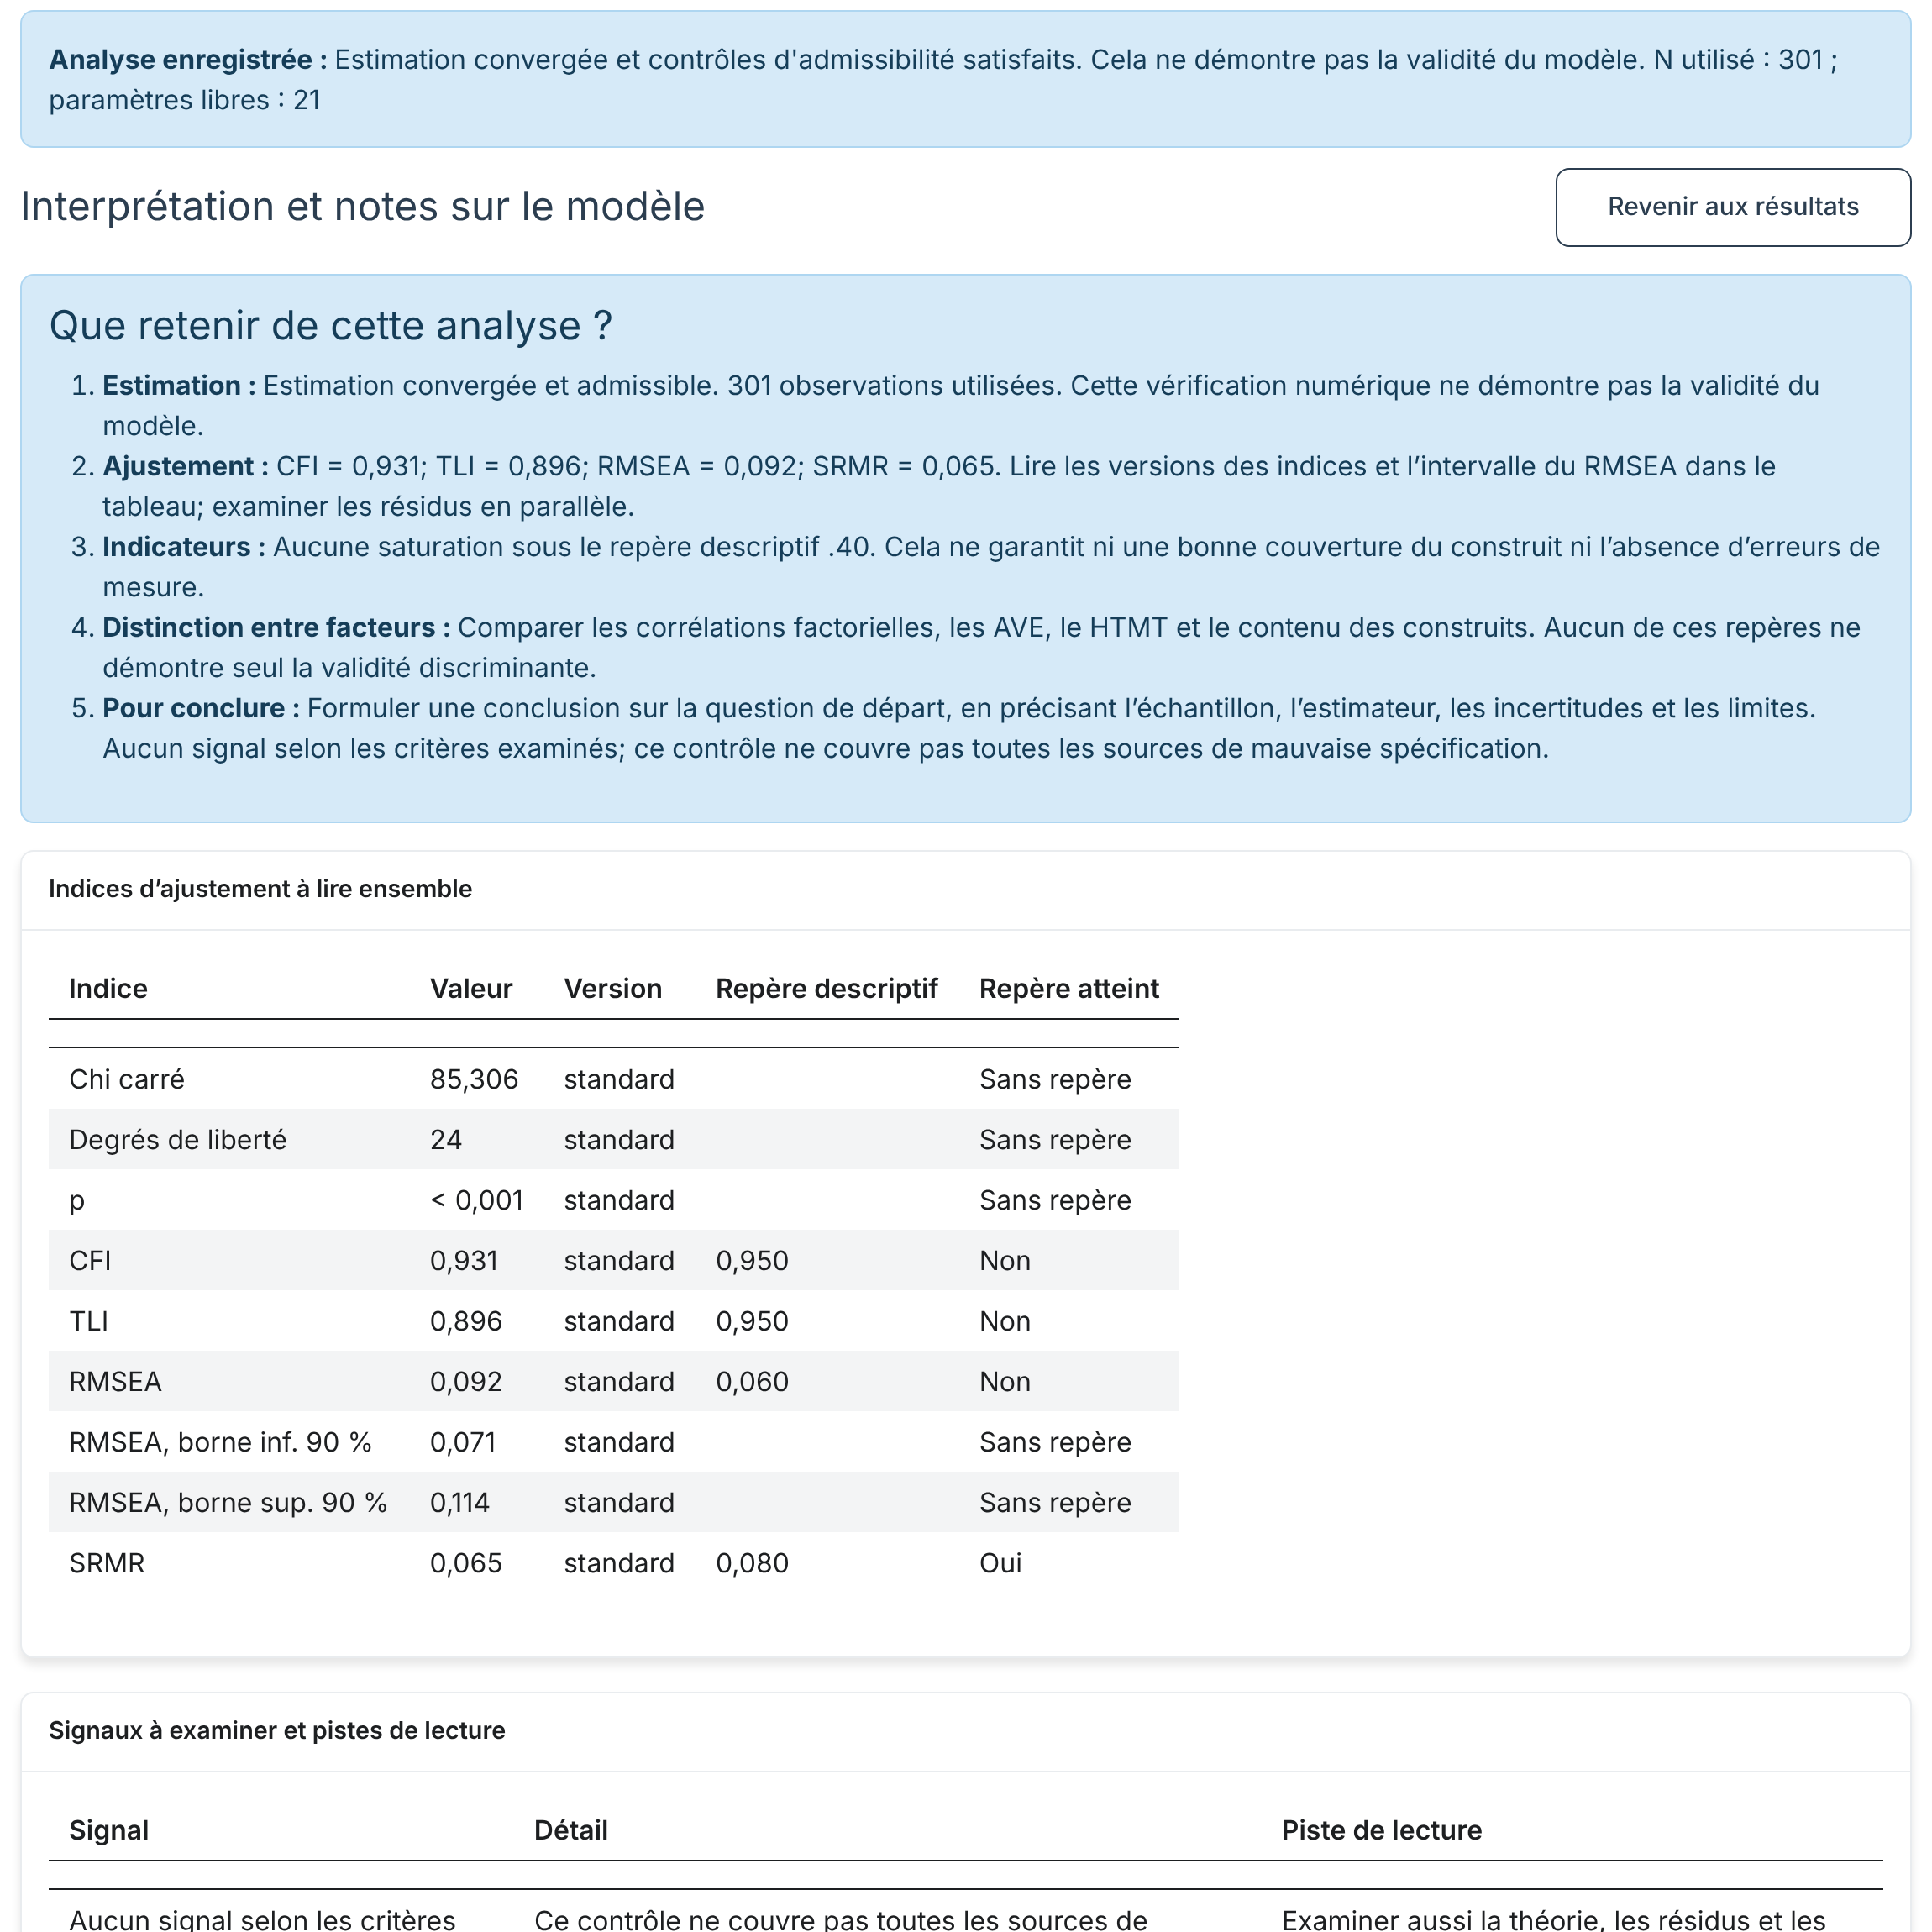
\includegraphics[width=1\linewidth,height=\textheight,keepaspectratio]{images/app/ch04_interpreter.png}

}

\caption{\label{fig-app-interpreter}\textbf{4. Interpréter} sur le
modèle de référence : la synthèse « Que retenir de cette analyse ? »,
puis le tableau des indices avec leur version, le repère descriptif et
la mention atteint ou non.}

\end{figure}%

\section{CFI et TLI}\label{cfi-et-tli}

Le \textbf{CFI} évalue l'amélioration relative par rapport à un modèle
de comparaison très restrictif, usuellement un modèle d'indépendance. Le
\textbf{TLI} tient aussi compte de la complexité d'une manière
différente. Ils ne représentent pas des pourcentages de personnes
correctement classées ou d'items « valides ».

Des valeurs proches de 1 sont généralement recherchées. Les repères 0,90
et 0,95 sont souvent mentionnés, mais leur interprétation dépend
notamment des conditions de l'analyse. Un CFI élevé peut coexister avec
des écarts locaux importants; le modèle de comparaison influence aussi
la lecture. Ici, le CFI de 0,931 et le TLI de 0,896 restent sous le
repère de 0,95 affiché par l'application.

\section{RMSEA et son intervalle}\label{rmsea-et-son-intervalle}

Le \textbf{RMSEA} exprime une approximation de l'écart d'ajustement par
degré de liberté. Lisez sa valeur avec son intervalle de confiance. Un
intervalle large indique qu'une plage étendue d'écarts reste compatible
avec l'incertitude de l'estimation.

Les repères 0,06 et 0,08 sont courants. Ils ne définissent pas une
frontière naturelle entre deux états de validité. Le RMSEA est
particulièrement délicat avec peu de degrés de liberté ou certains
petits échantillons. Dans l'exemple HS, la valeur de 0,092 et
l'intervalle de 0,071 à 0,114 incitent à examiner sérieusement la
spécification : même la borne inférieure dépasse 0,06.

\section{SRMR}\label{srmr}

Le \textbf{SRMR} résume des écarts standardisés entre relations
observées et reproduites. Une faible valeur indique que ces écarts sont
en moyenne limités. Un repère fréquent est 0,08. Une moyenne ne décrit
cependant pas chaque paire d'indicateurs : quelques écarts importants
peuvent subsister derrière un résumé relativement modéré. Le SRMR de
0,065 est le seul des quatre indices à atteindre son repère dans cet
exemple.

Les propositions de seuils associées notamment à Hu et Bentler
proviennent de conditions d'étude déterminées. Elles soutiennent une
lecture conjointe de plusieurs indices; leur transformation en critères
universels détachés du contexte serait excessive
(\citeproc{ref-hu1999}{Hu et Bentler 1999}).

\section{Ce qui change avec une estimation
robuste}\label{ce-qui-change-avec-une-estimation-robuste}

La sortie peut présenter des résultats \textbf{Standard},
\textbf{Scaled} ou \textbf{Robust}. Ces termes ne sont pas des
synonymes. Une correction du test du chi carré et une correction d'un
indice dérivé ne sont pas nécessairement la même opération. Dans
\textbf{4. Interpréter}, la colonne de version permet de savoir quel
résultat est repris : l'application retient la version robuste
lorsqu'elle existe, puis la version \emph{scaled}, puis la version
standard.

Lorsque plusieurs versions sont disponibles, rapportez clairement celle
que vous utilisez. Ne prenez pas le CFI le plus favorable dans une
colonne et le RMSEA le plus favorable dans une autre sans l'indiquer.
Une différence entre les valeurs d'un tableau du manuel et celles de
votre écran peut provenir d'une version différente de l'indice, même si
le modèle est identique.

\textbf{ML robuste} correspond ici à MLR. Sur les mêmes données HS, il
donne exactement les mêmes saturations ponctuelles que ML, mais un chi
carré corrigé de 87,132 au lieu de 85,306, un CFI robuste de 0,930 et un
RMSEA robuste de 0,092. Les erreurs-types et les tests changent; la
structure estimée, non. La robustesse à certains écarts de distribution
ne corrige pas une mauvaise affectation des indicateurs aux facteurs
(\citeproc{ref-lavaanest}{Projet lavaan 2026c}).

\section{Revenir au modèle HS}\label{revenir-au-moduxe8le-hs}

Le diagnostic ne se résume pas à « bon » ou « mauvais ». Les
coefficients ont une organisation interprétable; pourtant, le chi carré,
le RMSEA et le TLI ne soutiennent pas une reproduction pleinement
satisfaisante. Le SRMR invite à nuancer l'ampleur moyenne des écarts,
sans les faire disparaître.

Une formulation défendable est : « Le modèle à trois facteurs présente
une solution admissible et des saturations cohérentes avec
l'organisation attendue. Les indices globaux indiquent cependant des
écarts qui justifient l'examen des résidus et du contenu des
indicateurs. » Cette conclusion prépare une investigation; elle ne
prescrit aucune modification automatique.

\section{Un modèle plus simple est-il aussi convaincant
?}\label{un-moduxe8le-plus-simple-est-il-aussi-convaincant}

Pour une comparaison descriptive, rechargez le même fichier, définissez
un seul facteur \texttt{General} et attribuez-lui \texttt{x1} à
\texttt{x9}. Conservez ML, les cas complets et l'indicateur de
référence. Estimez et comparez :

\Needspace{6\baselineskip}

{

\begin{longtable}[]{@{}lrrrr@{}}

\caption{\label{tbl-hs-un}Comparaison descriptive du modèle à trois
facteurs et du modèle à un facteur (ML, 301 élèves).}

\tabularnewline

\toprule\noalign{}
Modèle & ddl & CFI & RMSEA & SRMR \\
\midrule\noalign{}
\endhead
\bottomrule\noalign{}
\endlastfoot
Trois facteurs & 24 & 0,931 & 0,092 & 0,065 \\
Un facteur & 27 & 0,677 & 0,187 & 0,143 \\

\end{longtable}

}

\begin{figure}[htbp]

\centering{

\includegraphics[width=0.88\linewidth,height=\textheight,keepaspectratio]{04-ajustement_files/figure-pdf/fig-indices-modeles-1.png}

}

\caption{\label{fig-indices-modeles}Trois modèles pour les mêmes neuf
tests. Les lignes pointillées marquent les repères descriptifs de
l'application (CFI ≥ 0,95; RMSEA ≤ 0,06; SRMR ≤ 0,08). Le modèle à un
facteur s'écarte nettement; la covariance résiduelle x7--x8, discutée au
chapitre suivant, améliore surtout le CFI et le RMSEA.}

\end{figure}%

Le modèle à un facteur reproduit nettement moins bien les données : son
CFI tombe à 0,677 et son RMSEA monte à 0,187. Cette observation soutient
l'intérêt de distinguer les dimensions dans ce jeu. Elle ne suffit pas à
prouver que le modèle à trois facteurs est entièrement satisfaisant.

\textbf{N'appliquez pas une différence usuelle de chi carré entre ces
deux modèles par simple soustraction.} La fusion des facteurs correspond
à une limite de corrélation parfaite, qui pose une difficulté pour le
test usuel. L'application bloque ce raccourci dans les comparaisons
automatisées. Ici, la comparaison reste descriptive et substantielle.

\section{Laboratoire : annoter un
rapport}\label{laboratoire-annoter-un-rapport}

À partir du rapport \texttt{HS\_trois\_facteurs\_ML.html} téléchargé au
chapitre précédent, relevez le chi carré, les degrés de liberté, le CFI,
le TLI, le RMSEA avec son intervalle et le SRMR. Pour chaque valeur,
écrivez ce qu'elle renseigne et ce qu'elle ne peut pas démontrer.
Terminez par une conclusion intégrée de cinq lignes, sans employer
uniquement les mots « accepté » ou « rejeté ».

\begin{tcolorbox}[enhanced jigsaw, arc=.35mm, bottomrule=.15mm, bottomtitle=1mm, breakable, colback=white, colbacktitle=quarto-callout-tip-color!10!white, colframe=quarto-callout-tip-color-frame, coltitle=black, left=2mm, leftrule=.75mm, opacityback=0, opacitybacktitle=0.6, rightrule=.15mm, title={Réponse}, titlerule=0mm, toprule=.15mm, toptitle=1mm]

Repères : chi carré 85,306 pour 24 dl, p \textless{} 0,001 (l'ajustement
exact est rejeté, sans dire où ni de combien); CFI 0,931 et TLI 0,896
(amélioration relative par rapport à l'indépendance, sous le repère de
0,95); RMSEA 0,092, IC 90 \% {[}0,071; 0,114{]} (écart approximatif
nettement au-dessus de 0,06, même à la borne inférieure); SRMR 0,065
(écart moyen modéré, qui peut cacher des écarts locaux).

Une conclusion intégrée : « La structure à trois facteurs est admissible
et ses saturations sont cohérentes. Le chi carré, le CFI, le TLI et le
RMSEA indiquent toutefois des écarts que le SRMR, plus favorable, ne
fait pas disparaître. Ces écarts doivent être localisés dans les résidus
et confrontés au contenu des tests avant toute modification. Le modèle
reste nettement meilleur qu'un facteur unique. »

\end{tcolorbox}

\begin{tcolorbox}[enhanced jigsaw, arc=.35mm, bottomrule=.15mm, bottomtitle=1mm, breakable, colback=white, colbacktitle=quarto-callout-important-color!10!white, colframe=quarto-callout-important-color-frame, coltitle=black, left=2mm, leftrule=.75mm, opacityback=0, opacitybacktitle=0.6, rightrule=.15mm, title={À retenir}, titlerule=0mm, toprule=.15mm, toptitle=1mm]

\begin{itemize}
\tightlist
\item
  Convergence, admissibilité et ajustement sont trois contrôles
  distincts.
\item
  Les indices se lisent ensemble, avec leur version; aucun seuil ne
  tranche seul.
\item
  Le RMSEA se lit avec son intervalle; le SRMR est une moyenne qui peut
  masquer des écarts locaux.
\item
  Un estimateur robuste corrige les tests et les erreurs-types, pas une
  mauvaise structure.
\end{itemize}

\end{tcolorbox}

\section{Quiz}\label{quiz-3}

\begin{enumerate}
\def\labelenumi{\arabic{enumi}.}
\tightlist
\item
  Un modèle converge, mais une variance résiduelle est négative. Peut-on
  lire ses indices d'ajustement ?
\item
  Le chi carré est significatif avec 3 000 observations et un CFI de
  0,97. Que conclure ?
\item
  Deux rapports du même modèle donnent un RMSEA de 0,029 et de 0,079.
  Est-ce une erreur ?
\item
  Pourquoi ne pas tester le modèle à un facteur contre le modèle à trois
  facteurs par une simple différence de chi carré ?
\end{enumerate}

\begin{tcolorbox}[enhanced jigsaw, arc=.35mm, bottomrule=.15mm, bottomtitle=1mm, breakable, colback=white, colbacktitle=quarto-callout-tip-color!10!white, colframe=quarto-callout-tip-color-frame, coltitle=black, left=2mm, leftrule=.75mm, opacityback=0, opacitybacktitle=0.6, rightrule=.15mm, title={Réponses}, titlerule=0mm, toprule=.15mm, toptitle=1mm]

\begin{enumerate}
\def\labelenumi{\arabic{enumi}.}
\tightlist
\item
  Non. La solution est inadmissible; il faut d'abord comprendre la cause
  (spécification, identification, données).
\item
  Le test détecte des écarts que la grande taille d'échantillon rend
  visibles; le CFI suggère qu'ils sont modestes en relatif. Il faut
  localiser ces écarts avant de conclure.
\item
  Pas nécessairement : ce peut être la version standard et la version
  robuste du même indice. Il faut lire la colonne de version.
\item
  Le modèle à un facteur correspond à des corrélations entre facteurs
  fixées à 1, une valeur à la frontière de l'espace des paramètres : le
  test usuel n'y est pas valide.
\end{enumerate}

\end{tcolorbox}

\bookmarksetup{startatroot}

\chapter{Examiner les données et comprendre les
signaux}\label{sec-diagnostics}

\begin{tcolorbox}[enhanced jigsaw, arc=.35mm, bottomrule=.15mm, bottomtitle=1mm, breakable, colback=white, colbacktitle=quarto-callout-note-color!10!white, colframe=quarto-callout-note-color-frame, coltitle=black, left=2mm, leftrule=.75mm, opacityback=0, opacitybacktitle=0.6, rightrule=.15mm, title={Objectifs du chapitre}, titlerule=0mm, toprule=.15mm, toptitle=1mm]

\begin{itemize}
\tightlist
\item
  Utiliser les statistiques descriptives et la carte des corrélations
  pour répondre à une question précise.
\item
  Interpréter les tests de normalité sans en faire un vote.
\item
  Examiner les observations éloignées sans les supprimer mécaniquement.
\item
  Localiser les écarts du modèle par les résidus et les indices de
  modification.
\end{itemize}

\end{tcolorbox}

\begin{tcolorbox}[enhanced jigsaw, arc=.35mm, bottomrule=.15mm, bottomtitle=1mm, breakable, colback=white, colbacktitle=quarto-callout-tip-color!10!white, colframe=quarto-callout-tip-color-frame, coltitle=black, left=2mm, leftrule=.75mm, opacityback=0, opacitybacktitle=0.6, rightrule=.15mm, title={Idée centrale}, titlerule=0mm, toprule=.15mm, toptitle=1mm]

Un indice global dit \emph{si} le modèle s'écarte des données; les
résidus et les indices de modification disent \emph{où}. Aucun
diagnostic n'autorise une modification par lui-même : il pose une
question que le contenu des indicateurs doit trancher.

\end{tcolorbox}

\section{Une inspection qui répond à des
questions}\label{une-inspection-qui-ruxe9pond-uxe0-des-questions}

Les diagnostics sont utiles lorsqu'ils éclairent une difficulté précise
: variable mal codée, dispersion insuffisante, relation inattendue,
distribution particulière ou écart entre deux indicateurs que le modèle
ne reproduit pas. Parcourir mécaniquement tous les tests sans revenir à
la question de mesure produit beaucoup de résultats et peu
d'information.

Pour suivre ce chapitre, rechargez le modèle HS à trois facteurs. Avant
d'estimer, fixez \textbf{Indices de modification : seuil} à 10 dans
\textbf{Modèle \& Spécification} : la section sur les indices de
modification en aura besoin. Estimez ensuite avec les réglages de la
première analyse.

\section{Statistiques univariées et
distributions}\label{statistiques-univariuxe9es-et-distributions}

Dans \textbf{Statistiques Descriptives → Univariées}, examinez le nombre
d'observations disponibles, la dispersion et les valeurs extrêmes. Une
variable constante ne peut pas contribuer normalement à une analyse de
covariance. Une valeur hors de l'échelle prévue doit d'abord être
vérifiée dans la documentation du fichier.

\begin{figure}[htbp]

\centering{

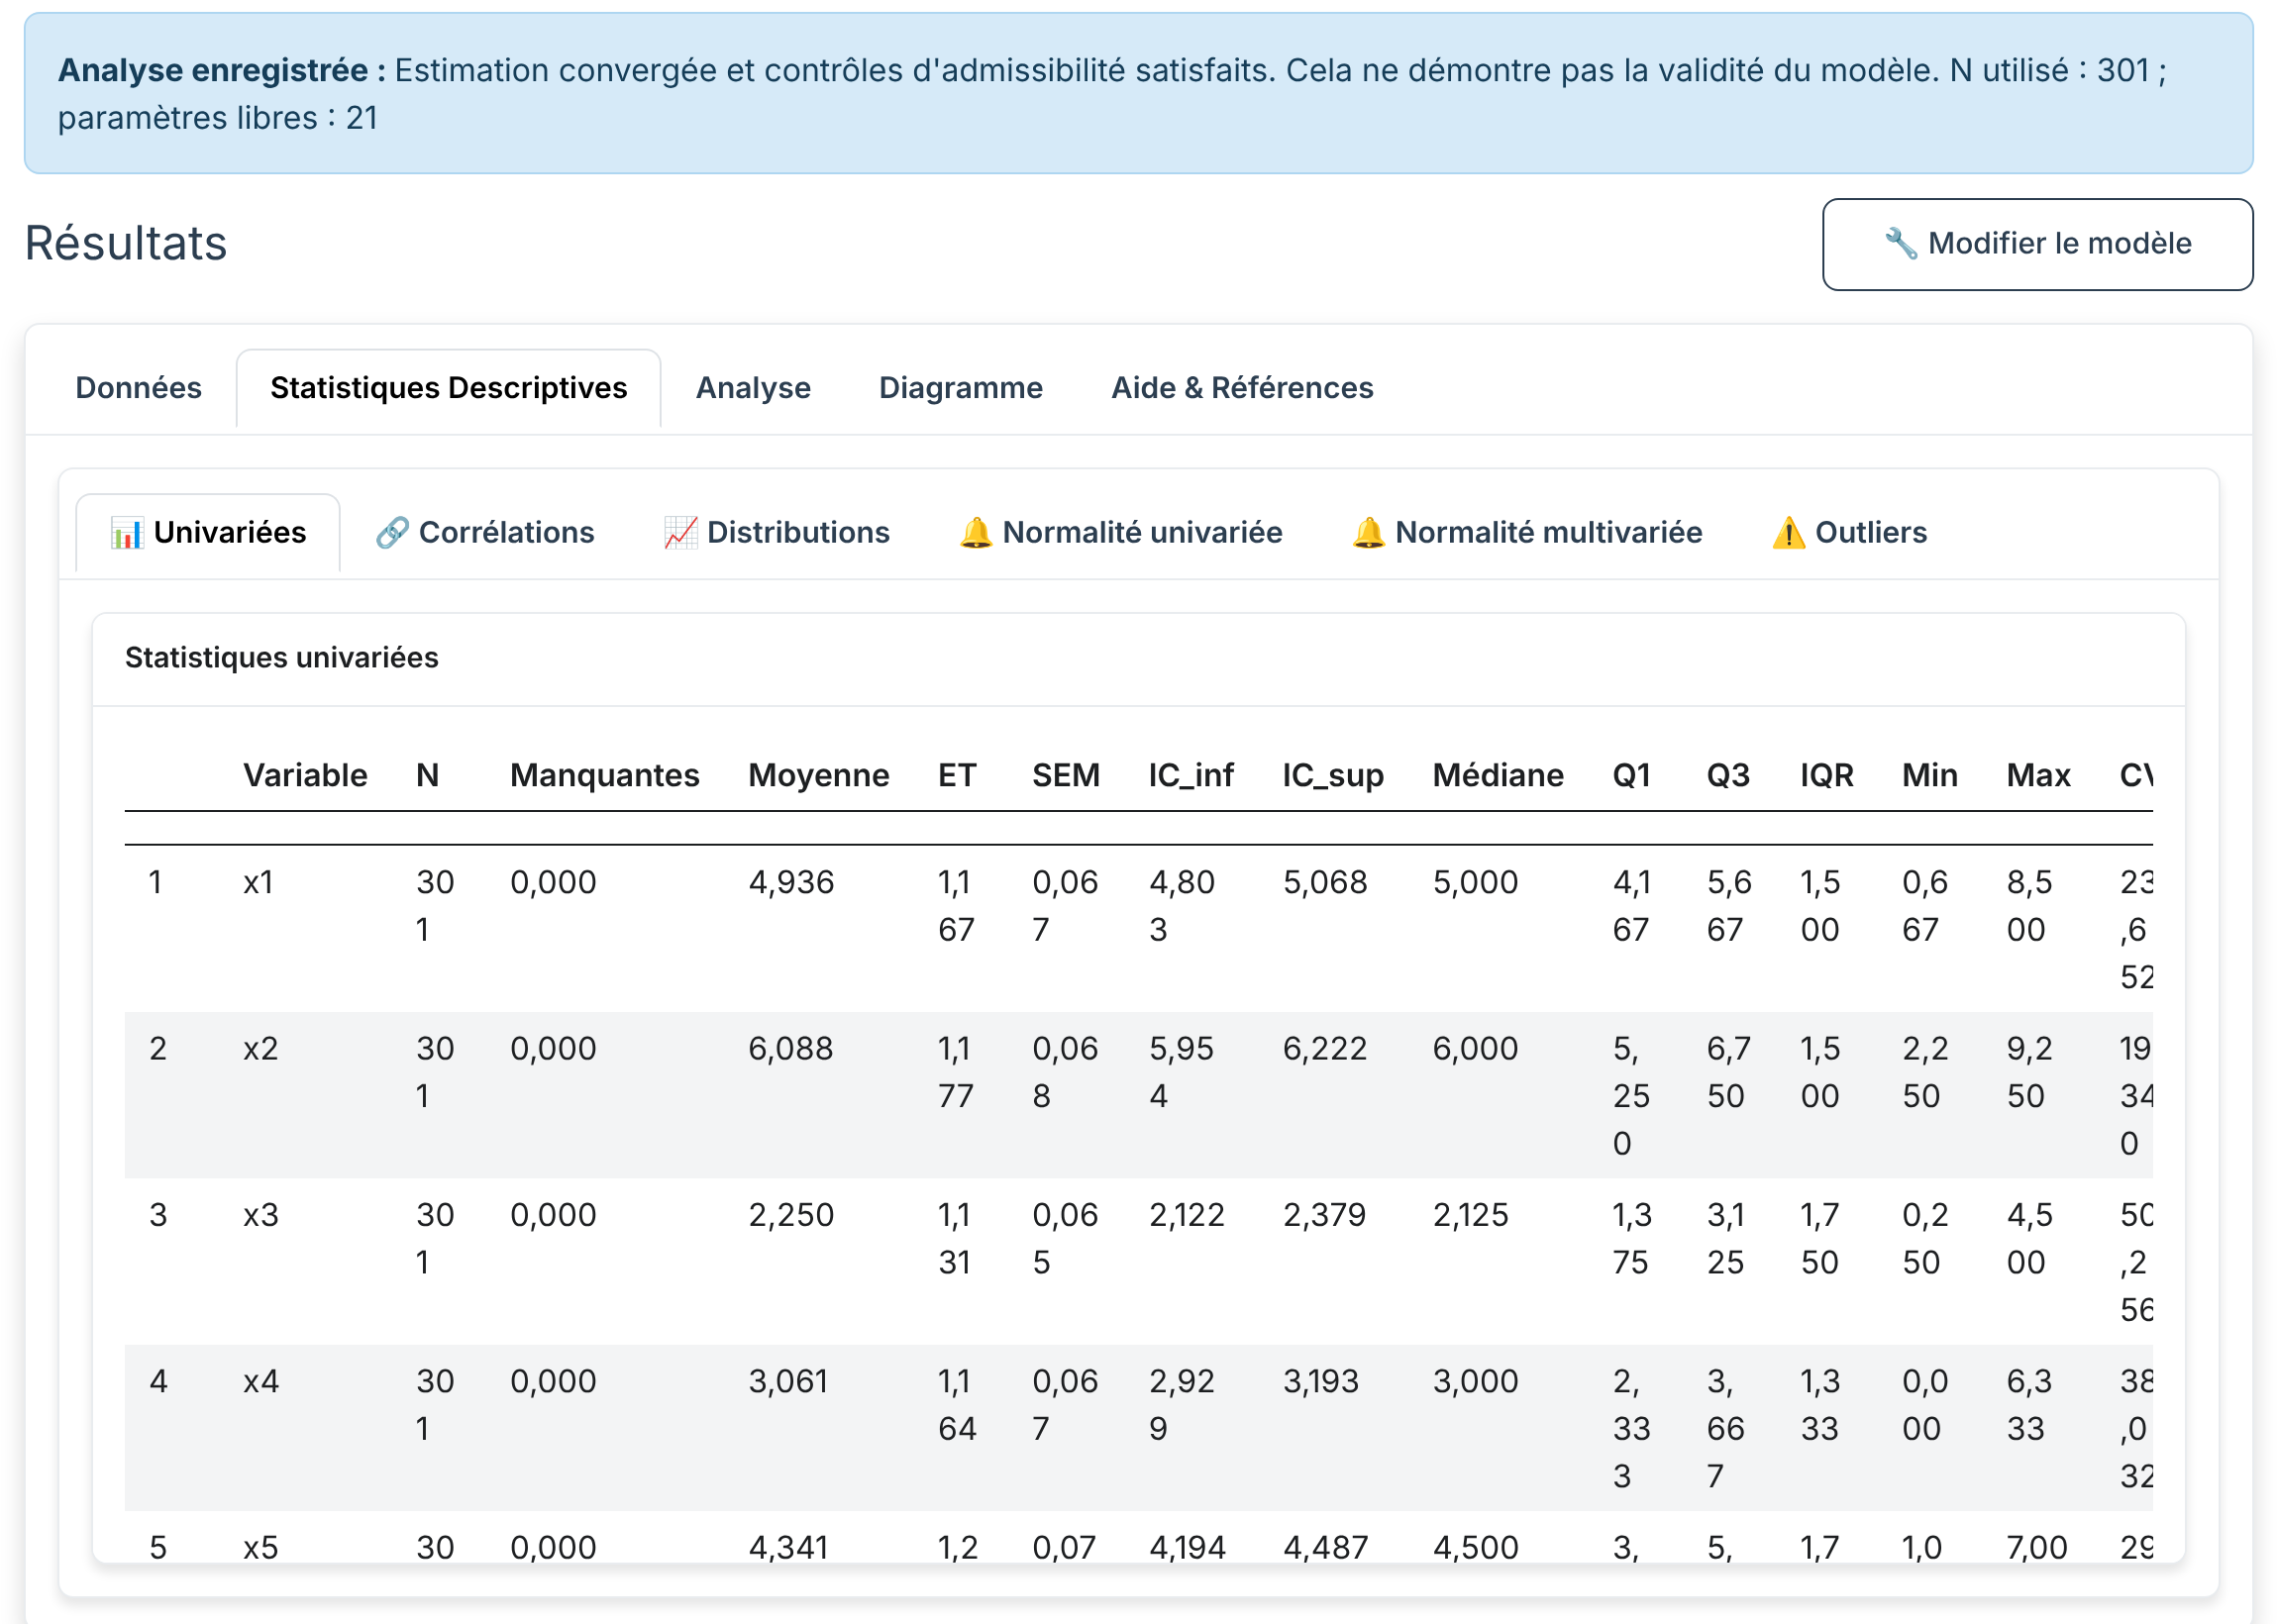
\includegraphics[width=1\linewidth,height=\textheight,keepaspectratio]{images/app/ch05_univariees.png}

}

\caption{\label{fig-app-univariees}\textbf{Statistiques Descriptives →
Univariées} : effectif, valeurs manquantes, moyenne, dispersion,
quantiles, asymétrie et aplatissement de chaque indicateur.}

\end{figure}%

Dans \textbf{Distributions}, sélectionnez les variables et le type de
graphique. L'histogramme montre la répartition en classes; la densité
donne une représentation lissée; la boîte à moustaches aide à repérer la
position, la dispersion et certaines observations éloignées. L'aspect
dépend aussi de l'échelle et des choix graphiques. Une distribution
visuellement asymétrique n'est pas une faute de saisie par définition.

Ne mélangez pas les variables de nature différente. Les catégories 0 à 3
d'un adjectif du MSQ n'ont pas à ressembler à une courbe continue
normale. Leur inspection appelle d'abord une réflexion sur les
catégories, leur fréquence et leur ordre.

\section{La carte des corrélations}\label{la-carte-des-corruxe9lations}

Dans \textbf{Corrélations}, le triangle supérieur utilise des couleurs
et le triangle inférieur affiche les coefficients. Le signe doit rester
lisible : une forte relation négative est forte en valeur absolue, mais
son sens est opposé à celui d'une relation positive.

\begin{figure}[htbp]

\centering{

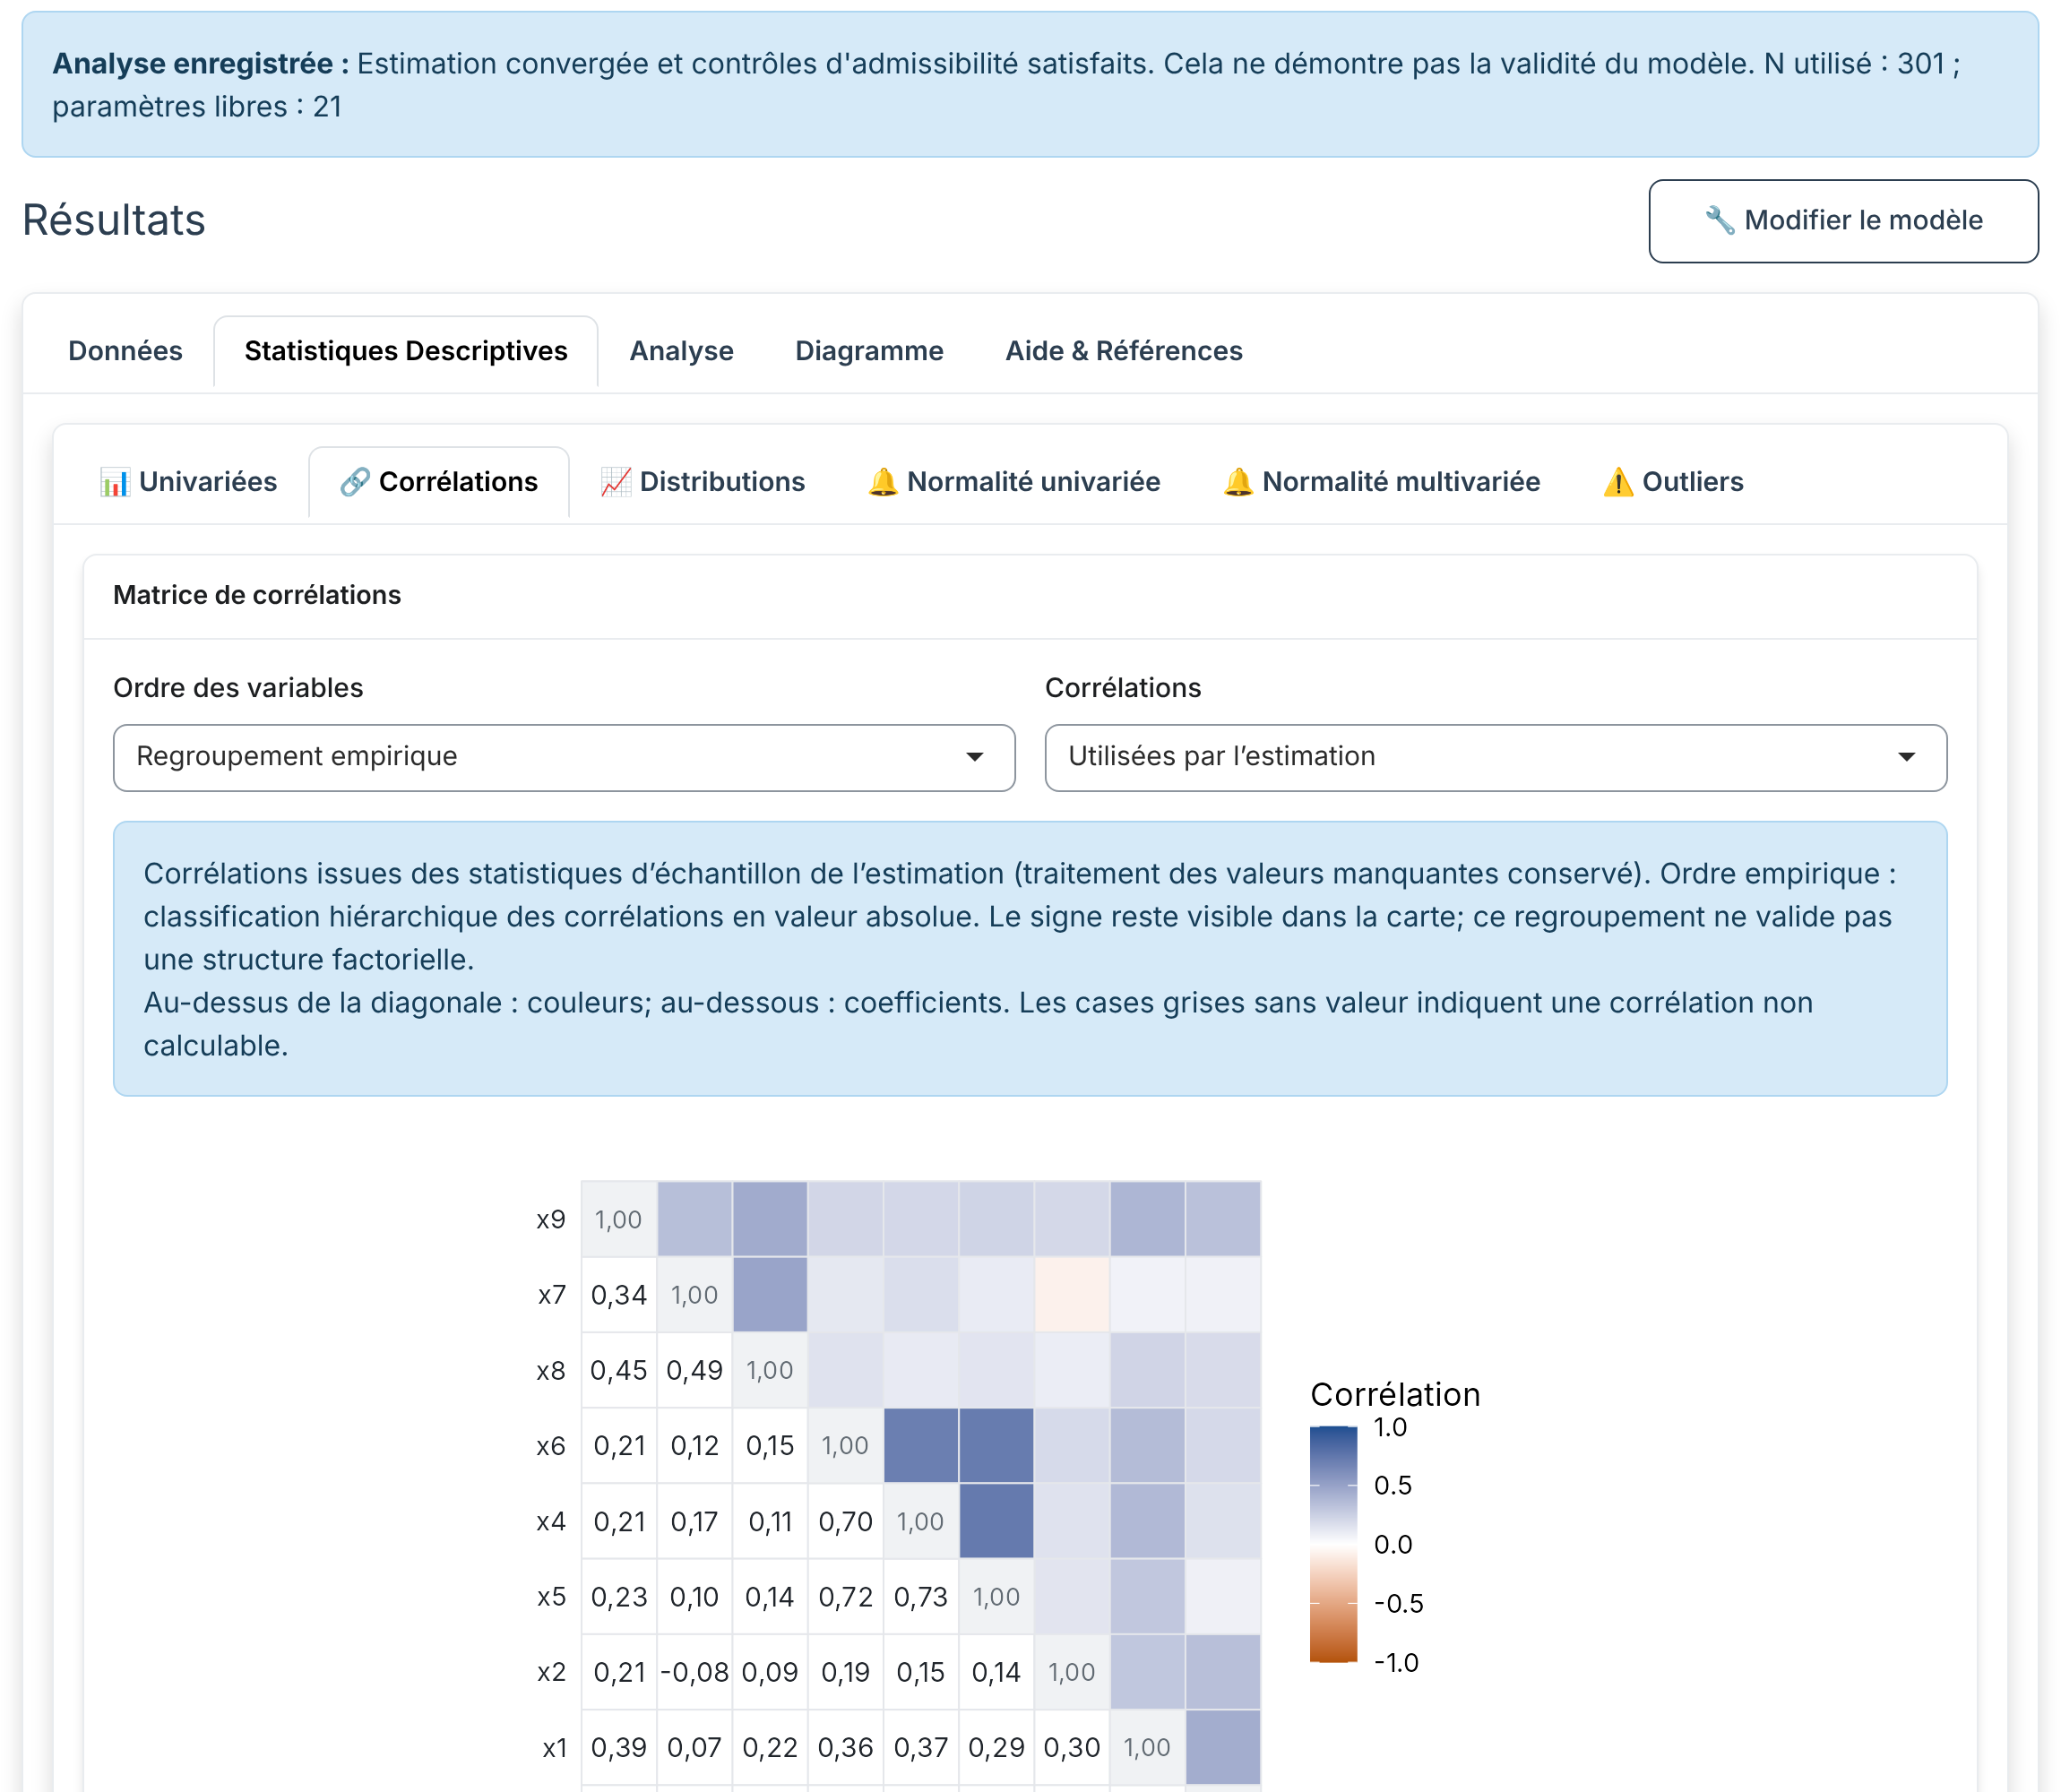
\includegraphics[width=1\linewidth,height=\textheight,keepaspectratio]{images/app/ch05_correlations.png}

}

\caption{\label{fig-app-correlations}\textbf{Statistiques Descriptives →
Corrélations} en regroupement empirique. Les trois blocs de tests
apparaissent, mais les relations entre blocs ne sont pas nulles.}

\end{figure}%

L'ordre peut suivre un \textbf{regroupement empirique}, les
\textbf{facteurs définis} ou l'\textbf{ordre d'origine}. Le regroupement
empirique rapproche les variables selon les corrélations en valeur
absolue. Il peut donc rapprocher deux items de sens opposé. Il ne
constitue pas une analyse factorielle exploratoire ni une preuve que les
facteurs annoncés sont les bons.

Choisissez aussi la base des corrélations. Les corrélations
\textbf{utilisées par l'estimation} peuvent être polychoriques ou
polysériales avec des variables ordinales; les corrélations de
\textbf{Pearson} portent sur les scores numériques observés. Une
différence entre ces bases n'est pas nécessairement une erreur de
calcul. Annoncez celle que vous décrivez.

\section{Normalité univariée}\label{normalituxe9-univariuxe9e}

L'onglet réunit \textbf{Shapiro--Wilk}, \textbf{Lilliefors} et
\textbf{Anderson--Darling} pour les indicateurs continus. Leurs
hypothèses et sensibilités diffèrent. L'absence de rejet ne prouve pas
que la population est normale. Plusieurs tests sur plusieurs indicateurs
augmentent aussi la possibilité de rencontrer une petite valeur de p.

Sur les neuf tests HS, Shapiro--Wilk rejette la normalité à 0,05 pour 6
indicateurs. Les asymétries restent pourtant modestes, de −0,35 à 0,86,
et l'aplatissement le plus marqué vaut 1,17 (x8). Avec 301 élèves, de
petits écarts suffisent à faire rejeter le test : la taille de l'écart
compte davantage que la valeur de p.

\begin{figure}[htbp]

\centering{

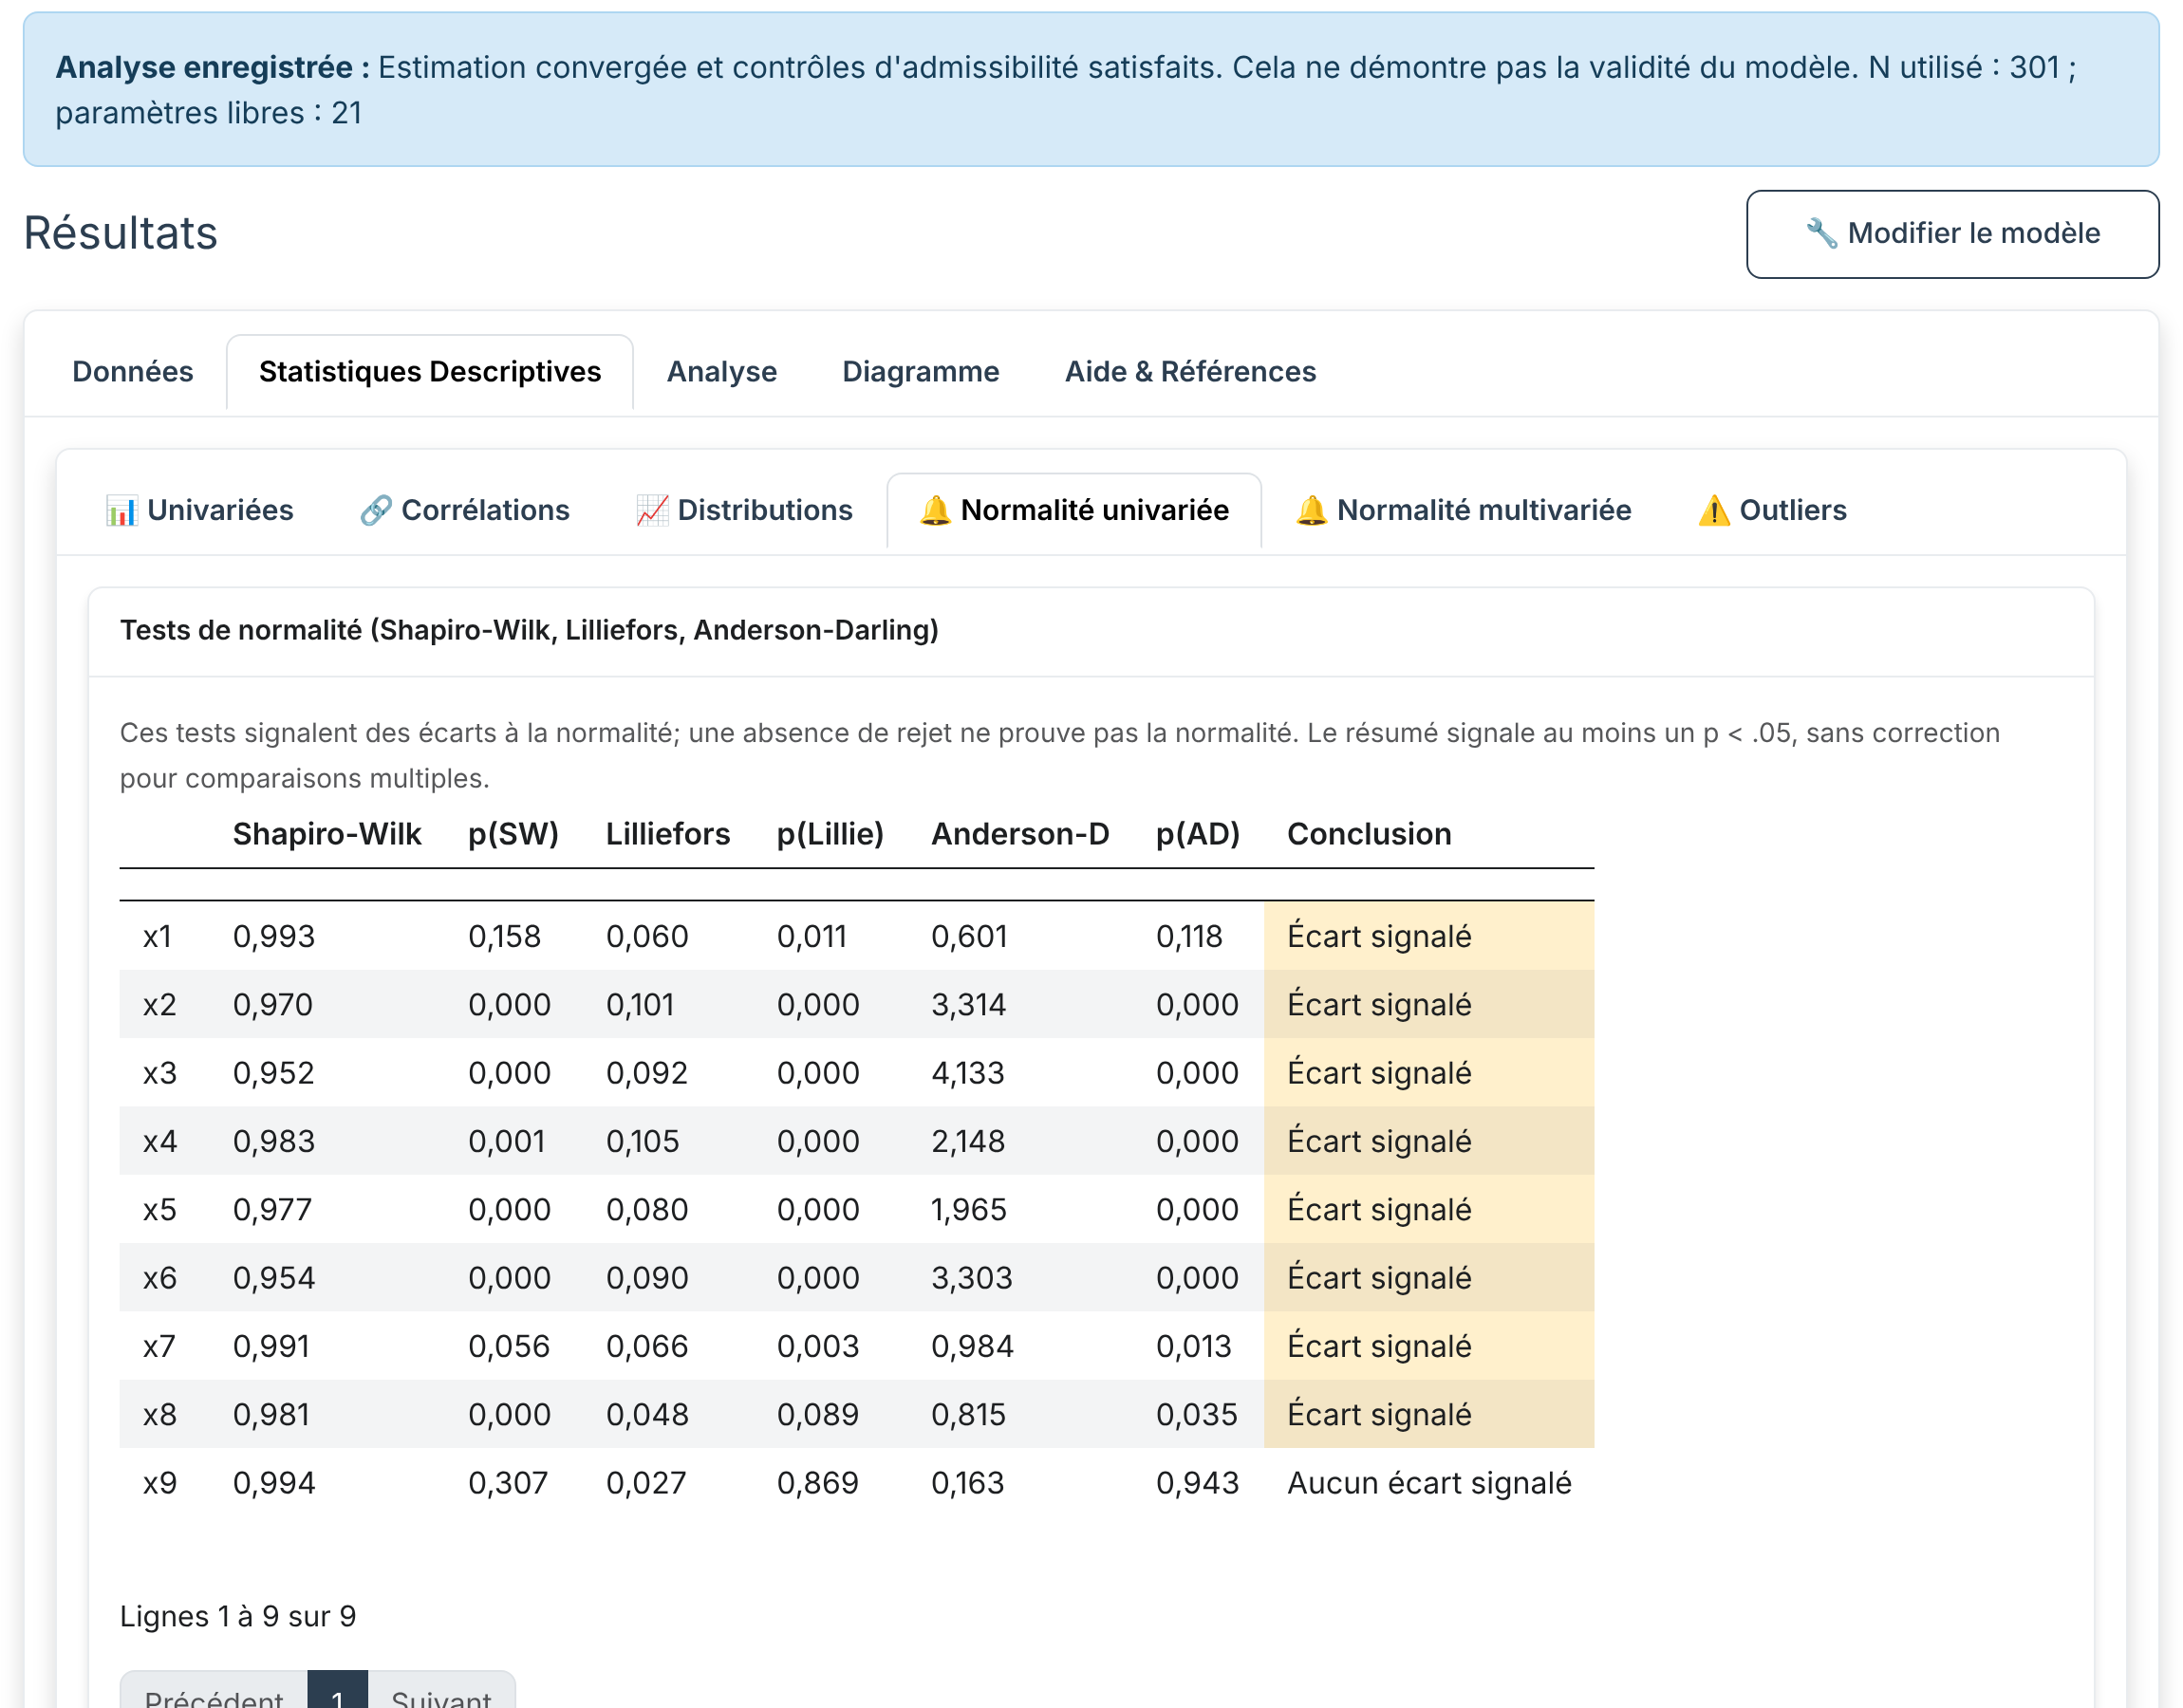
\includegraphics[width=1\linewidth,height=\textheight,keepaspectratio]{images/app/ch05_normalite_uni.png}

}

\caption{\label{fig-app-normuni}\textbf{Normalité univariée} : trois
tests par indicateur, avec leur statistique et leur valeur de p.}

\end{figure}%

Certains tests imposent des conditions d'effectif. Par exemple,
Shapiro--Wilk n'est pas calculé ici au-delà de 5 000 observations
disponibles pour un indicateur. Une case non calculée n'est pas un
résultat favorable. Les tests utilisent les valeurs non manquantes de
chaque indicateur : leur effectif peut varier d'une variable à l'autre.

\textbf{Lorsque tous les indicateurs sont déclarés ordinaux, une note
remplace le tableau.} Aucun test continu de normalité n'est calculé sur
leurs catégories. Pour un modèle mixte, seules les variables continues
apparaissent dans le tableau et une note annonce l'exclusion des
variables ordinales.

\section{Normalité multivariée}\label{normalituxe9-multivariuxe9e}

La normalité de chaque variable ne suffit pas à garantir la normalité
conjointe. L'onglet \textbf{Normalité multivariée} réunit cinq méthodes
: Henze--Zirkler, Mardia, Royston, Doornik--Hansen et Énergie. Mardia
comporte deux volets, asymétrie et aplatissement, d'où la possibilité
d'obtenir six lignes pour cinq méthodes.

\Needspace{10\baselineskip}

{

\begin{longtable}[]{@{}
  >{\raggedright\arraybackslash}p{(\linewidth - 8\tabcolsep) * \real{0.2027}}
  >{\raggedright\arraybackslash}p{(\linewidth - 8\tabcolsep) * \real{0.1892}}
  >{\raggedleft\arraybackslash}p{(\linewidth - 8\tabcolsep) * \real{0.1622}}
  >{\raggedright\arraybackslash}p{(\linewidth - 8\tabcolsep) * \real{0.1081}}
  >{\raggedright\arraybackslash}p{(\linewidth - 8\tabcolsep) * \real{0.3378}}@{}}

\caption{\label{tbl-hs-mvn}Normalité multivariée des neuf tests HS (301
cas complets), telle que la présente l'application.}

\tabularnewline

\toprule\noalign{}
\begin{minipage}[b]{\linewidth}\raggedright
Méthode
\end{minipage} & \begin{minipage}[b]{\linewidth}\raggedright
Volet
\end{minipage} & \begin{minipage}[b]{\linewidth}\raggedleft
Statistique
\end{minipage} & \begin{minipage}[b]{\linewidth}\raggedright
p
\end{minipage} & \begin{minipage}[b]{\linewidth}\raggedright
Lecture
\end{minipage} \\
\midrule\noalign{}
\endhead
\bottomrule\noalign{}
\endlastfoot
Henze--Zirkler & Global & 1,054 & \textless{} 0,001 & Écart signalé (p
\textless{} 0,05) \\
Mardia & Asymétrie & 344,905 & \textless{} 0,001 & Écart signalé (p
\textless{} 0,05) \\
Mardia & Aplatissement & 2,830 & 0,005 & Écart signalé (p \textless{}
0,05) \\
Royston & Global & 125,972 & \textless{} 0,001 & Écart signalé (p
\textless{} 0,05) \\
Doornik--Hansen & Global & 134,618 & \textless{} 0,001 & Écart signalé
(p \textless{} 0,05) \\
Énergie & Global & 2,131 & \textless{} 0,001 & Écart signalé (p
\textless{} 0,05) \\

\end{longtable}

}

Les méthodes sont appliquées au même ensemble de cas complets. Le nombre
utilisé est indiqué. Si une méthode est indisponible ou ne peut pas être
calculée, son statut doit être lu comme tel. L'absence du package
facultatif requis dans l'environnement ne constitue pas une conclusion
sur les données.

Ces diagnostics ne forment pas un vote : trois tests non significatifs
contre deux significatifs ne « prouveraient » pas la normalité. Sur HS,
6 lignes sur 6 signalent un écart; cette concordance justifie de garder
à l'esprit l'option \textbf{ML robuste} présentée au chapitre précédent.
Avec des indicateurs ordinaux, les tests continus ne sont pas
applicables. L'analyse ordinale repose sur un modèle de réponses
latentes qui n'exige pas une distribution normale des catégories
observées.

\section{Observations éloignées}\label{observations-uxe9loignuxe9es}

L'onglet \textbf{Outliers} propose la distance de Mahalanobis et une
variante robuste fondée sur MCD. Ces diagnostics examinent des positions
multivariées inhabituelles. Leur interprétation est surtout adaptée ici
aux indicateurs continus. Un motif rare de catégories ordinales ne doit
pas être supprimé mécaniquement sur la base de ces distances.

Avec le seuil de probabilité par défaut de 0,001 et neuf indicateurs, la
distance critique vaut 27,88. Sur HS, la distance classique signale 2
élèves et la variante robuste en signale 9. L'écart entre les deux n'est
pas une contradiction : la version robuste estime le centre et la
dispersion sans se laisser tirer par les observations les plus
éloignées, si bien qu'elle en repère davantage.

\begin{figure}[htbp]

\centering{

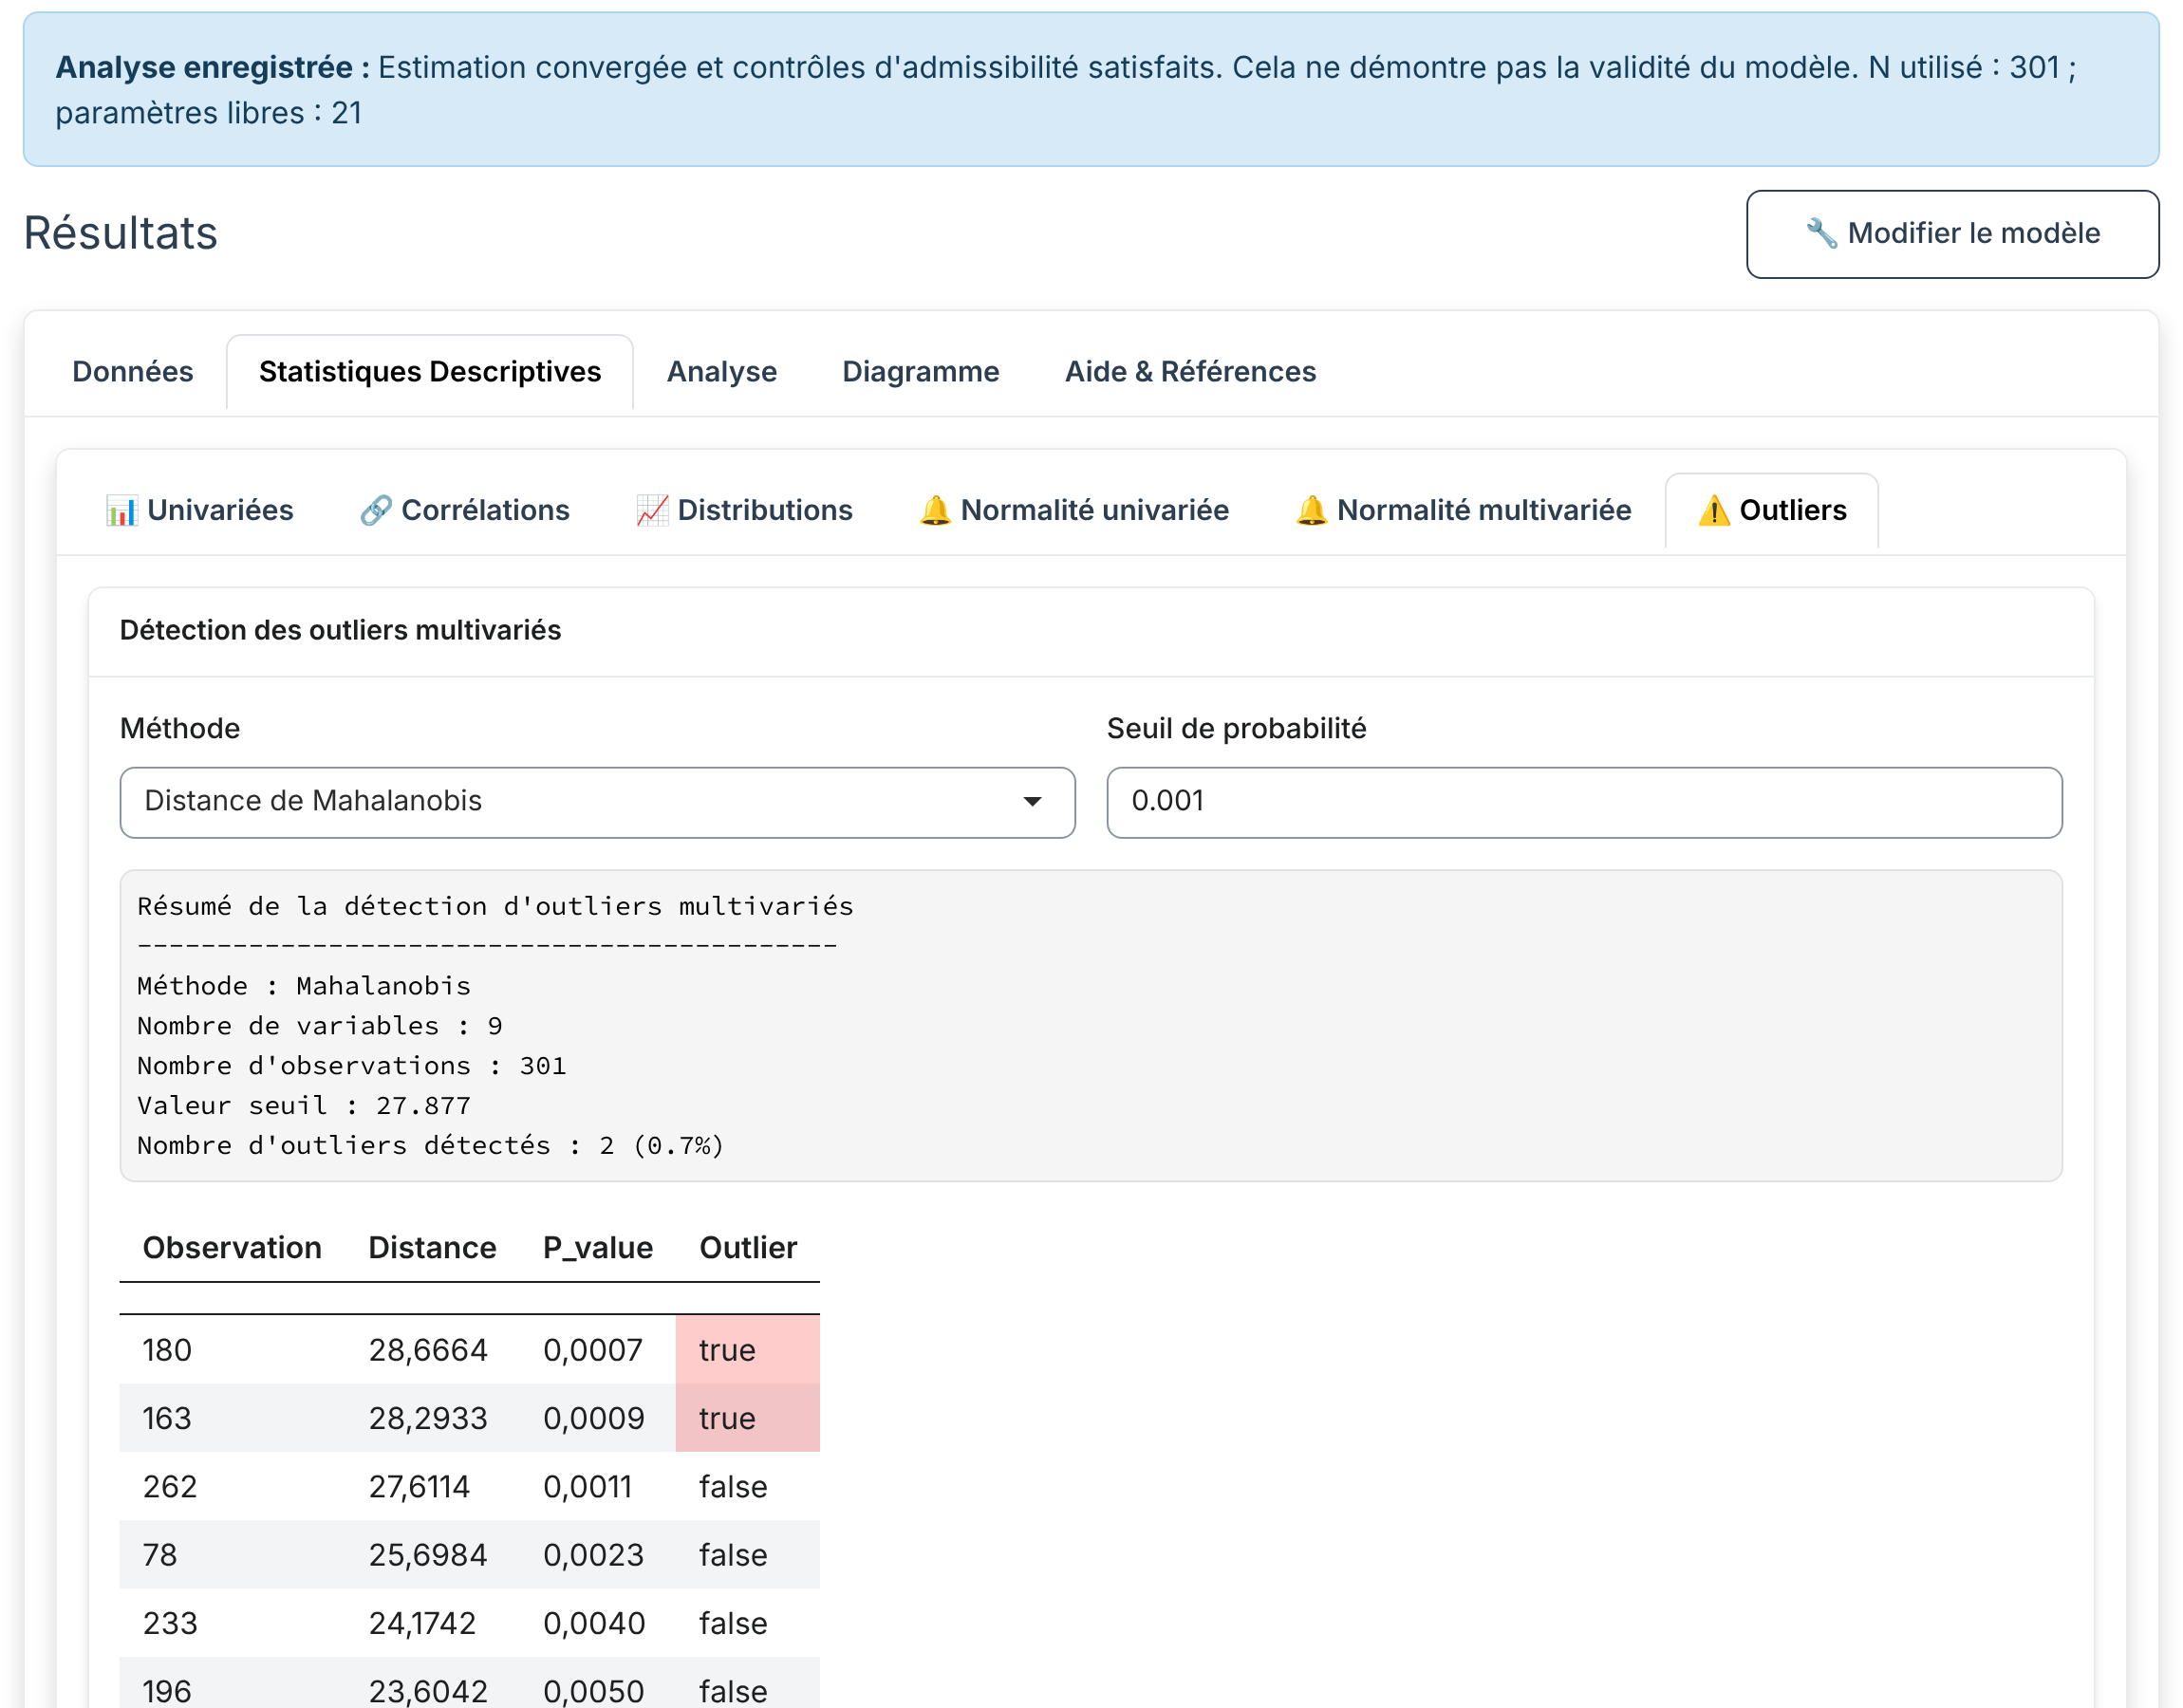
\includegraphics[width=1\linewidth,height=\textheight,keepaspectratio]{images/app/ch05_outliers.png}

}

\caption{\label{fig-app-outliers}\textbf{Outliers} : méthode, seuil de
probabilité, résumé et tableau des observations signalées.}

\end{figure}%

Le calcul utilise des cas complets et nécessite une covariance
exploitable. L'effectif peut donc différer de celui d'une estimation
FIML. Le repère issu du chi carré, particulièrement pour la variante
robuste, reste un repère d'approximation. Une petite valeur de p est une
invitation à vérifier, pas une autorisation de supprimer une personne.

Avant toute exclusion, demandez-vous si la valeur est impossible, si
elle provient d'une erreur documentée ou si elle représente une
observation réelle. Consignez la règle et comparez les conclusions avec
et sans l'exclusion lorsque cette comparaison est justifiée.

\section{Résidus du modèle}\label{ruxe9sidus-du-moduxe8le}

Les matrices observées résument les relations dans les données; les
matrices implicites décrivent celles que le modèle reproduit. Un résidu
met en évidence leur différence dans la métrique choisie. Les résidus de
corrélation et leurs valeurs standardisées ne se lisent pas avec les
mêmes unités.

Dans \textbf{Modèle \& Spécification → Affichage des résultats et
matrices}, cochez les matrices souhaitées (\textbf{Covariances} et
\textbf{Corrélations} : observée, implicite, résiduelle, résiduelle
standardisée), puis revenez à \textbf{Analyse → Analyse de base →
Matrices}. Les choix de matrices et le seuil des indices de modification
changent la présentation de l'analyse enregistrée, sans réestimer ses
paramètres. À l'inverse, modifier la structure, la nature des
indicateurs, l'estimateur ou la gestion des absences nécessite une
nouvelle estimation.

\begin{figure}[htbp]

\centering{

\includegraphics[width=0.88\linewidth,height=\textheight,keepaspectratio]{05-diagnostics_files/figure-pdf/fig-residus-1.png}

}

\caption{\label{fig-residus}Résidus de corrélation du modèle de
référence (corrélation observée moins corrélation reproduite). Les cases
encadrées dépassent 0,10 en valeur absolue. Les plus grands écarts
relient deux tests de vitesse aux tests visuels : positifs pour x9 (le
modèle sous-estime ces relations), négatifs pour x7 (il les surestime).}

\end{figure}%

Un résidu positif entre deux indicateurs signifie que le modèle
reproduit moins de relation qu'il n'en est observé pour cette paire; un
résidu négatif, qu'il en reproduit trop. Sur HS, le plus grand résidu de
corrélation concerne x7 et x2 (−0,189), suivi de x5--x3 (−0,151) et de
x9--x1 (0,149). Parmi les 36 résidus standardisés, 14 dépassent 1,96 en
valeur absolue. Examinez les intitulés de la matrice pour savoir s'il
s'agit de covariances, de corrélations ou de résidus standardisés. Ne
comparez pas directement un nombre dans une matrice brute à un seuil
destiné à une valeur z.

\section{Indices de modification}\label{indices-de-modification}

Un indice de modification estime localement l'amélioration possible du
chi carré si un paramètre actuellement restreint était libéré.
L'\textbf{EPC} décrit le changement de paramètre attendu. Les colonnes
standardisées donnent d'autres échelles de lecture. Une valeur élevée ne
fournit pas une justification théorique (\citeproc{ref-lavaanmi}{Projet
lavaan 2026d}).

Pour afficher ce panneau, fixez \textbf{Indices de modification : seuil}
à 10 plutôt qu'à \texttt{Inf}, estimez, puis ouvrez \textbf{Analyse de
base → Indices de modification}. \texttt{Inf} masque ces indices; ce
n'est pas un seuil de significativité.

\Needspace{8\baselineskip}

{

\begin{longtable}[]{@{}lllrrr@{}}

\caption{\label{tbl-hs-mi}Indices de modification supérieurs à 10 pour
le modèle de référence. EPC : changement attendu du paramètre; EPC std :
sa version entièrement standardisée.}

\tabularnewline

\toprule\noalign{}
Gauche & Op. & Droite & MI & EPC & EPC std \\
\midrule\noalign{}
\endhead
\bottomrule\noalign{}
\endlastfoot
Visuel & =\textasciitilde{} & x9 & 36,411 & 0,577 & 0,515 \\
x7 & \textsubscript{} & x8 & 34,145 & 0,536 & 0,859 \\
Visuel & =\textasciitilde{} & x7 & 18,631 & −0,422 & −0,349 \\
x8 & \textsubscript{} & x9 & 14,946 & −0,423 & −0,805 \\

\end{longtable}

}

\begin{figure}[htbp]

\centering{

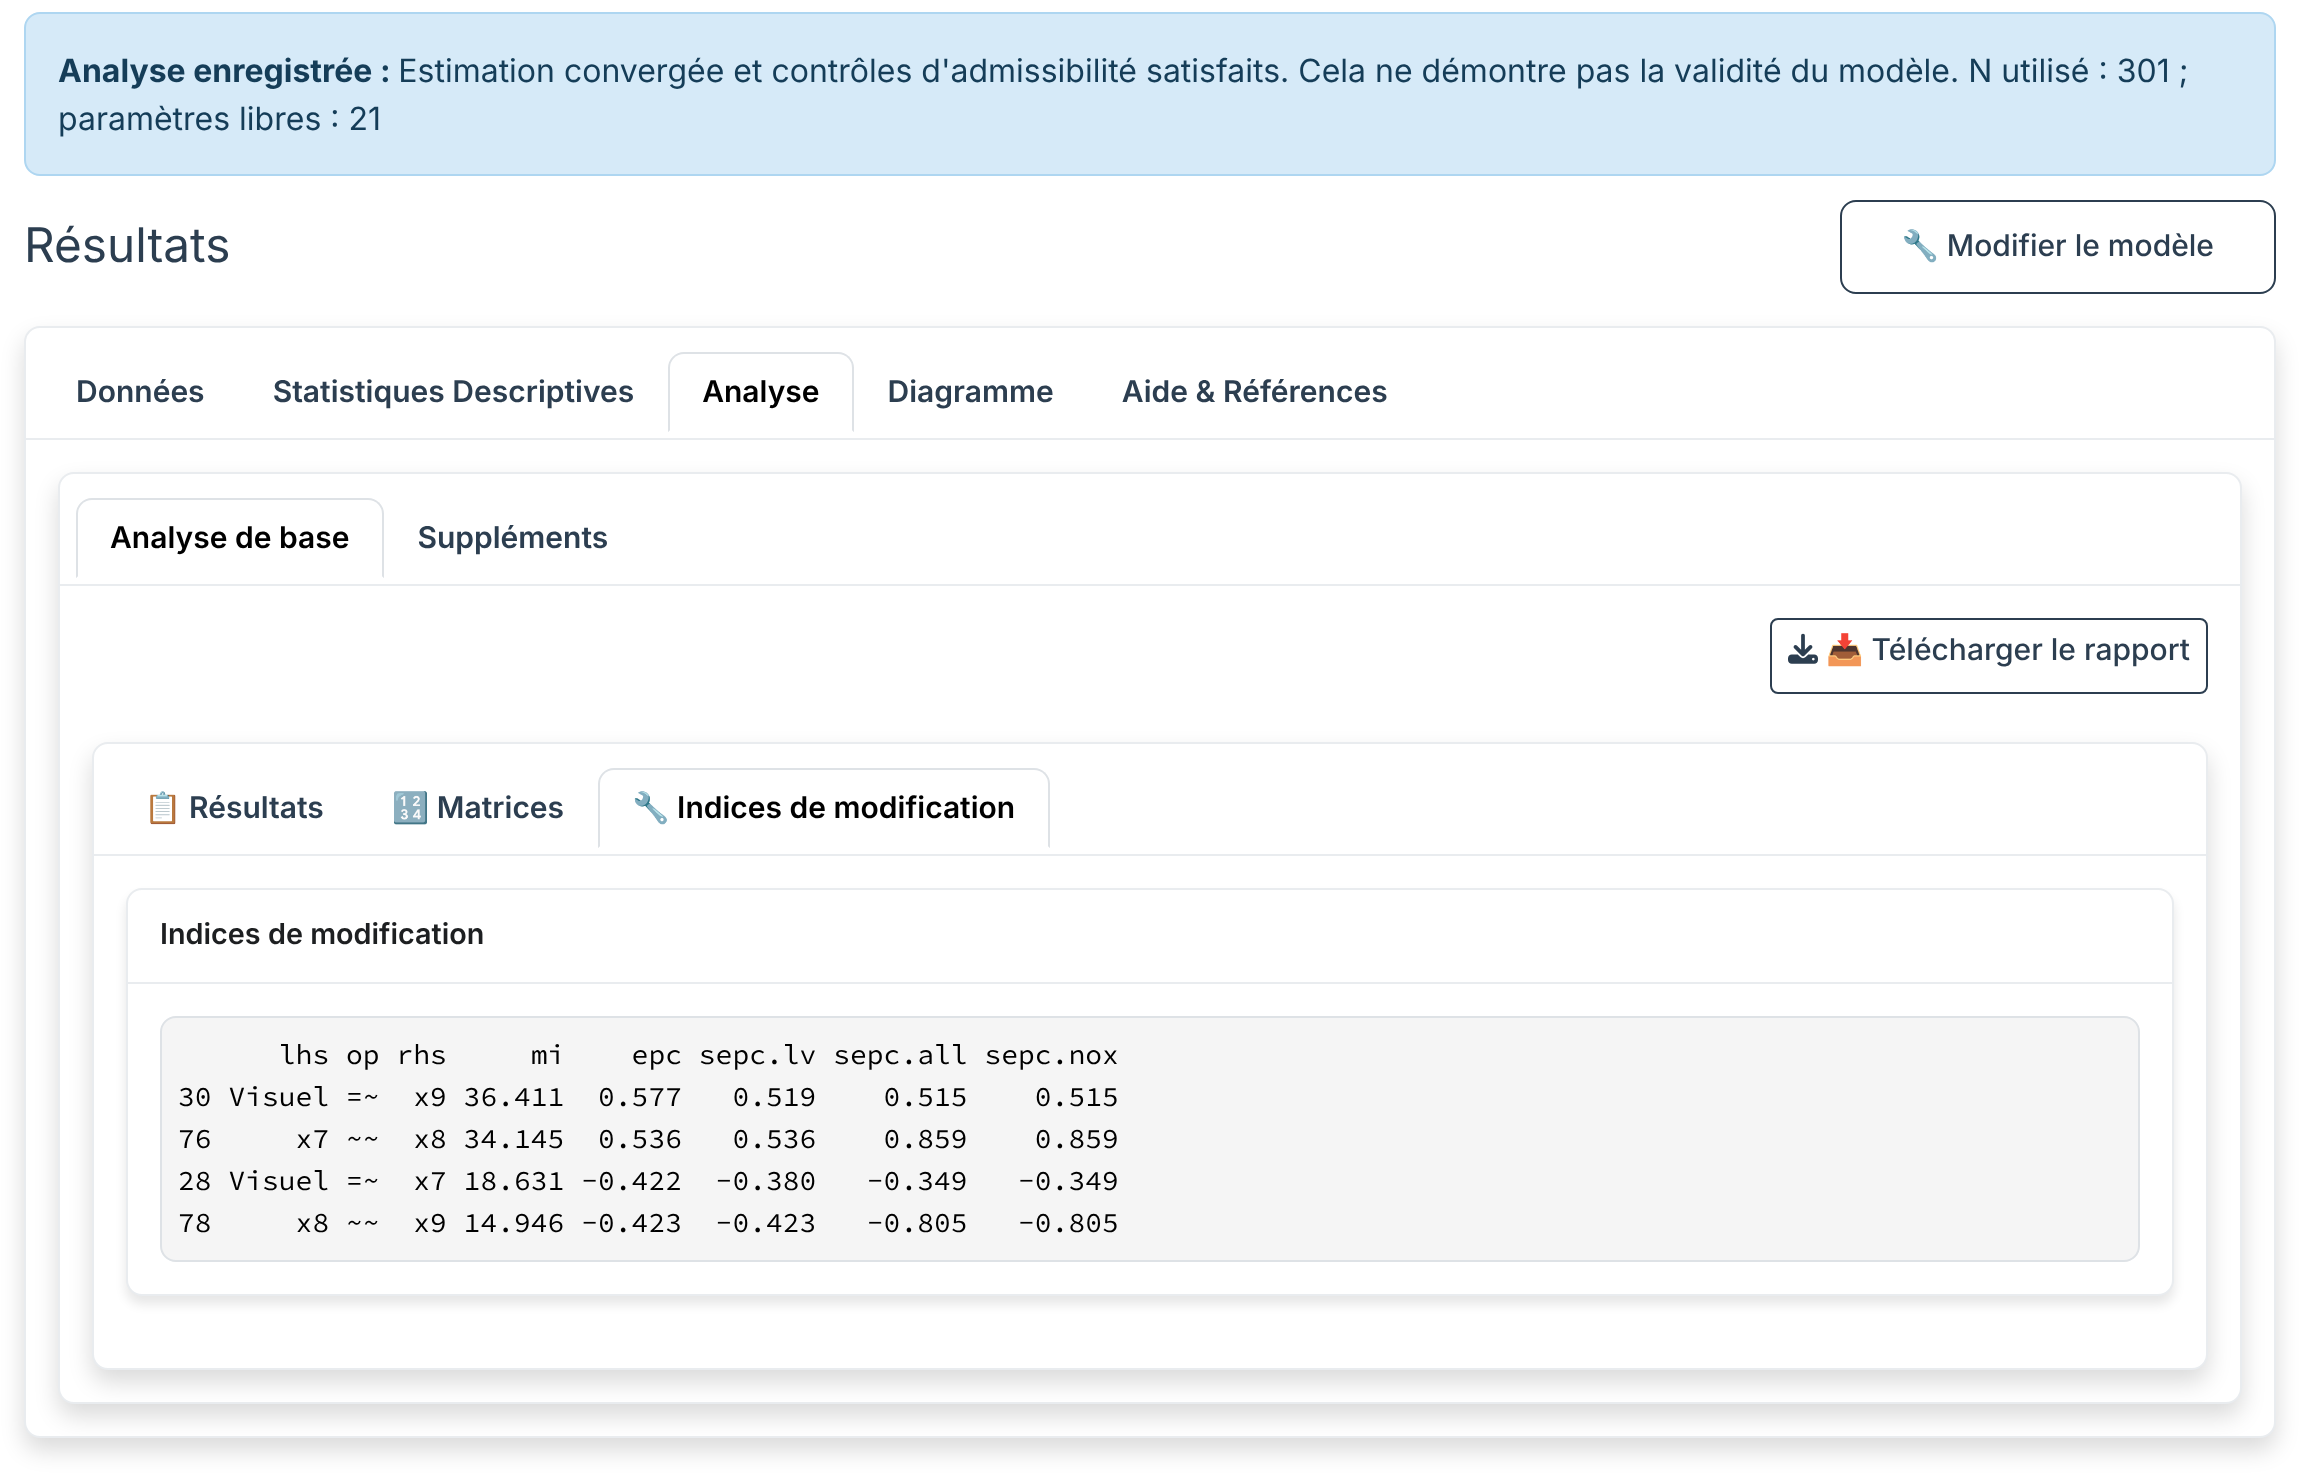
\includegraphics[width=1\linewidth,height=\textheight,keepaspectratio]{images/app/ch05_mi.png}

}

\caption{\label{fig-app-mi}\textbf{Analyse de base → Indices de
modification} avec un seuil de 10.}

\end{figure}%

Sur HS, deux propositions dominent : une saturation croisée de
\texttt{x9} sur le facteur visuel (MI = 36,4) et une covariance
résiduelle entre \texttt{x7} et \texttt{x8} (MI = 34,1). Elles racontent
deux histoires différentes. La première dit que la discrimination rapide
de lettres demande aussi une aptitude visuelle; la seconde, que
l'addition et le comptage rapides partagent quelque chose que le facteur
vitesse ne contient pas, par exemple un format de tâche chronométrée.
Écrivez d'abord ce qu'une telle modification signifierait. Ajouter
successivement toutes les propositions élevées adapte le modèle à cet
échantillon et peut réduire sa portée confirmatoire.

\section{Laboratoire : localiser un
écart}\label{laboratoire-localiser-un-uxe9cart}

\begin{enumerate}
\def\labelenumi{\arabic{enumi}.}
\tightlist
\item
  Sur le modèle HS, cochez les corrélations \textbf{Résiduelle} et
  \textbf{Résiduelle Std} dans \textbf{Affichage des résultats et
  matrices}, fixez le seuil des indices de modification à 10, puis
  estimez.
\item
  Repérez la paire d'indicateurs dont le résidu de corrélation est le
  plus grand en valeur absolue.
\item
  Comparez avec les deux plus grands indices de modification.
\item
  Choisissez l'une des deux modifications proposées et rédigez en deux
  phrases la justification de contenu qu'elle exigerait.
\end{enumerate}

\begin{tcolorbox}[enhanced jigsaw, arc=.35mm, bottomrule=.15mm, bottomtitle=1mm, breakable, colback=white, colbacktitle=quarto-callout-tip-color!10!white, colframe=quarto-callout-tip-color-frame, coltitle=black, left=2mm, leftrule=.75mm, opacityback=0, opacitybacktitle=0.6, rightrule=.15mm, title={Réponse}, titlerule=0mm, toprule=.15mm, toptitle=1mm]

Le plus grand résidu touche x7 et x2 (−0,189). Les deux plus grands
indices de modification proposent
\texttt{Visuel\ =\textasciitilde{}\ x9} (36,4) et
\texttt{x7\ \textasciitilde{}\textasciitilde{}\ x8} (34,1). Les deux
lectures concordent : le bloc vitesse est le moins bien reproduit.

Pour \texttt{x7\ \textasciitilde{}\textasciitilde{}\ x8} : « L'addition
et le comptage de points sont deux tâches chronométrées d'exécution
simple et répétitive; une composante de vitesse d'exécution propre à ce
format pourrait les lier au-delà du facteur général de vitesse. Cette
relation n'était pas prévue et devrait être vérifiée dans un autre
échantillon. » Le chapitre sur les contraintes montre comment l'ajouter
et ce qu'elle change.

\end{tcolorbox}

\begin{tcolorbox}[enhanced jigsaw, arc=.35mm, bottomrule=.15mm, bottomtitle=1mm, breakable, colback=white, colbacktitle=quarto-callout-important-color!10!white, colframe=quarto-callout-important-color-frame, coltitle=black, left=2mm, leftrule=.75mm, opacityback=0, opacitybacktitle=0.6, rightrule=.15mm, title={À retenir}, titlerule=0mm, toprule=.15mm, toptitle=1mm]

\begin{itemize}
\tightlist
\item
  Un diagnostic répond à une question; il ne vote pas et n'autorise
  aucune modification automatique.
\item
  Avec un effectif important, les tests de normalité rejettent de petits
  écarts : regardez l'ampleur.
\item
  Une observation éloignée se vérifie avant de s'exclure.
\item
  Résidus et indices de modification localisent les écarts; le contenu
  décide.
\end{itemize}

\end{tcolorbox}

\section{Quiz}\label{quiz-4}

\begin{enumerate}
\def\labelenumi{\arabic{enumi}.}
\tightlist
\item
  Le regroupement empirique de la carte des corrélations confirme-t-il
  la structure à trois facteurs ?
\item
  Les tests de normalité multivariée rejettent tous l'hypothèse. Faut-il
  abandonner l'AFC ?
\item
  Le seuil des indices de modification est à \texttt{Inf}. Le modèle
  n'a-t-il donc aucun écart local ?
\item
  Un indice de modification vaut 36. Suffit-il pour ajouter le paramètre
  ?
\end{enumerate}

\begin{tcolorbox}[enhanced jigsaw, arc=.35mm, bottomrule=.15mm, bottomtitle=1mm, breakable, colback=white, colbacktitle=quarto-callout-tip-color!10!white, colframe=quarto-callout-tip-color-frame, coltitle=black, left=2mm, leftrule=.75mm, opacityback=0, opacitybacktitle=0.6, rightrule=.15mm, title={Réponses}, titlerule=0mm, toprule=.15mm, toptitle=1mm]

\begin{enumerate}
\def\labelenumi{\arabic{enumi}.}
\tightlist
\item
  Non. Il réordonne les variables selon leurs corrélations; il ne teste
  pas un modèle.
\item
  Non. On peut employer un estimateur robuste et vérifier que les
  conclusions tiennent; l'écart de distribution n'invalide pas la
  structure.
\item
  Non. \texttt{Inf} masque simplement le tableau.
\item
  Non. Il indique un gain d'ajustement possible; le paramètre doit avoir
  un sens substantiel et sa découverte a posteriori doit être annoncée.
\end{enumerate}

\end{tcolorbox}

\bookmarksetup{startatroot}

\chapter{Comprendre ce que les indices de fiabilité
évaluent}\label{sec-fiabilite}

\begin{tcolorbox}[enhanced jigsaw, arc=.35mm, bottomrule=.15mm, bottomtitle=1mm, breakable, colback=white, colbacktitle=quarto-callout-note-color!10!white, colframe=quarto-callout-note-color-frame, coltitle=black, left=2mm, leftrule=.75mm, opacityback=0, opacitybacktitle=0.6, rightrule=.15mm, title={Objectifs du chapitre}, titlerule=0mm, toprule=.15mm, toptitle=1mm]

\begin{itemize}
\tightlist
\item
  Préciser le score dont on évalue la fiabilité : somme brute,
  combinaison pondérée ou réponse latente.
\item
  Distinguer alpha, oméga (CR), H et AVE, et lire leurs écarts.
\item
  Comprendre l'effet d'une covariance résiduelle et des items inversés
  sur la fiabilité d'une somme.
\item
  Situer les repères 0,70 et 0,50 par rapport à l'usage visé.
\end{itemize}

\end{tcolorbox}

\begin{tcolorbox}[enhanced jigsaw, arc=.35mm, bottomrule=.15mm, bottomtitle=1mm, breakable, colback=white, colbacktitle=quarto-callout-tip-color!10!white, colframe=quarto-callout-tip-color-frame, coltitle=black, left=2mm, leftrule=.75mm, opacityback=0, opacitybacktitle=0.6, rightrule=.15mm, title={Idée centrale}, titlerule=0mm, toprule=.15mm, toptitle=1mm]

« Quelle est la fiabilité ? » est une question incomplète. Il faut
d'abord dire \textbf{de quel score} : la somme des items, une somme
pondérée ou la réponse latente. Chaque indice répond pour un score
différent; leurs écarts renseignent sur les indicateurs.

\end{tcolorbox}

\section{La question porte sur un
score}\label{la-question-porte-sur-un-score}

Une structure factorielle et un score fiable sont deux questions liées,
mais distinctes. Le modèle décrit les relations entre les indicateurs.
La fiabilité concerne la proportion de variance attribuable à la
composante visée pour un score défini. Il faut donc préciser si l'on
parle d'une somme, d'une moyenne, d'une combinaison pondérée ou d'une
réponse latente.

Deux règles pratiques en découlent. D'abord, une fiabilité élevée ne
prouve pas l'unidimensionnalité. Ensuite, un indice fondé sur un modèle
dépend de la pertinence de ce modèle. Calculer une valeur très précise à
partir d'une structure mal spécifiée ne résout pas la difficulté de
mesure (\citeproc{ref-mcdonald1999}{McDonald 1999}).

\Needspace{8\baselineskip}

{\def\LTcaptype{none} % do not increment counter
\begin{longtable}[]{@{}
  >{\raggedright\arraybackslash}p{(\linewidth - 6\tabcolsep) * \real{0.2500}}
  >{\raggedright\arraybackslash}p{(\linewidth - 6\tabcolsep) * \real{0.2500}}
  >{\raggedright\arraybackslash}p{(\linewidth - 6\tabcolsep) * \real{0.2500}}
  >{\raggedright\arraybackslash}p{(\linewidth - 6\tabcolsep) * \real{0.2500}}@{}}
\toprule\noalign{}
\begin{minipage}[b]{\linewidth}\raggedright
Indice
\end{minipage} & \begin{minipage}[b]{\linewidth}\raggedright
Score visé
\end{minipage} & \begin{minipage}[b]{\linewidth}\raggedright
Calculé sur
\end{minipage} & \begin{minipage}[b]{\linewidth}\raggedright
Hypothèse principale
\end{minipage} \\
\midrule\noalign{}
\endhead
\bottomrule\noalign{}
\endlastfoot
Alpha & Somme des items observés & Covariances observées, cas complets &
Contributions égales des items, pas de covariance résiduelle \\
Oméga (CR) & Somme des items, dans leurs unités & Paramètres du modèle &
Le modèle de mesure est correct \\
H & Combinaison pondérée de façon optimale & Paramètres du modèle &
Idem; poids choisis par le modèle \\
AVE & Aucun score : moyenne par indicateur & Saturations standardisées &
Structure simple \\
\end{longtable}
}

\section{Où lire les résultats}\label{ouxf9-lire-les-ruxe9sultats}

Rechargez et estimez le modèle HS à trois facteurs. Dans \textbf{Analyse
→ Suppléments → Fiabilité}, le tableau présente notamment
\textbf{Alpha}, \textbf{Omega}, \textbf{CR}, \textbf{AVE} et \textbf{H}.
Les notes sous le tableau précisent la cible du calcul et les limites.

\begin{figure}[htbp]

\centering{

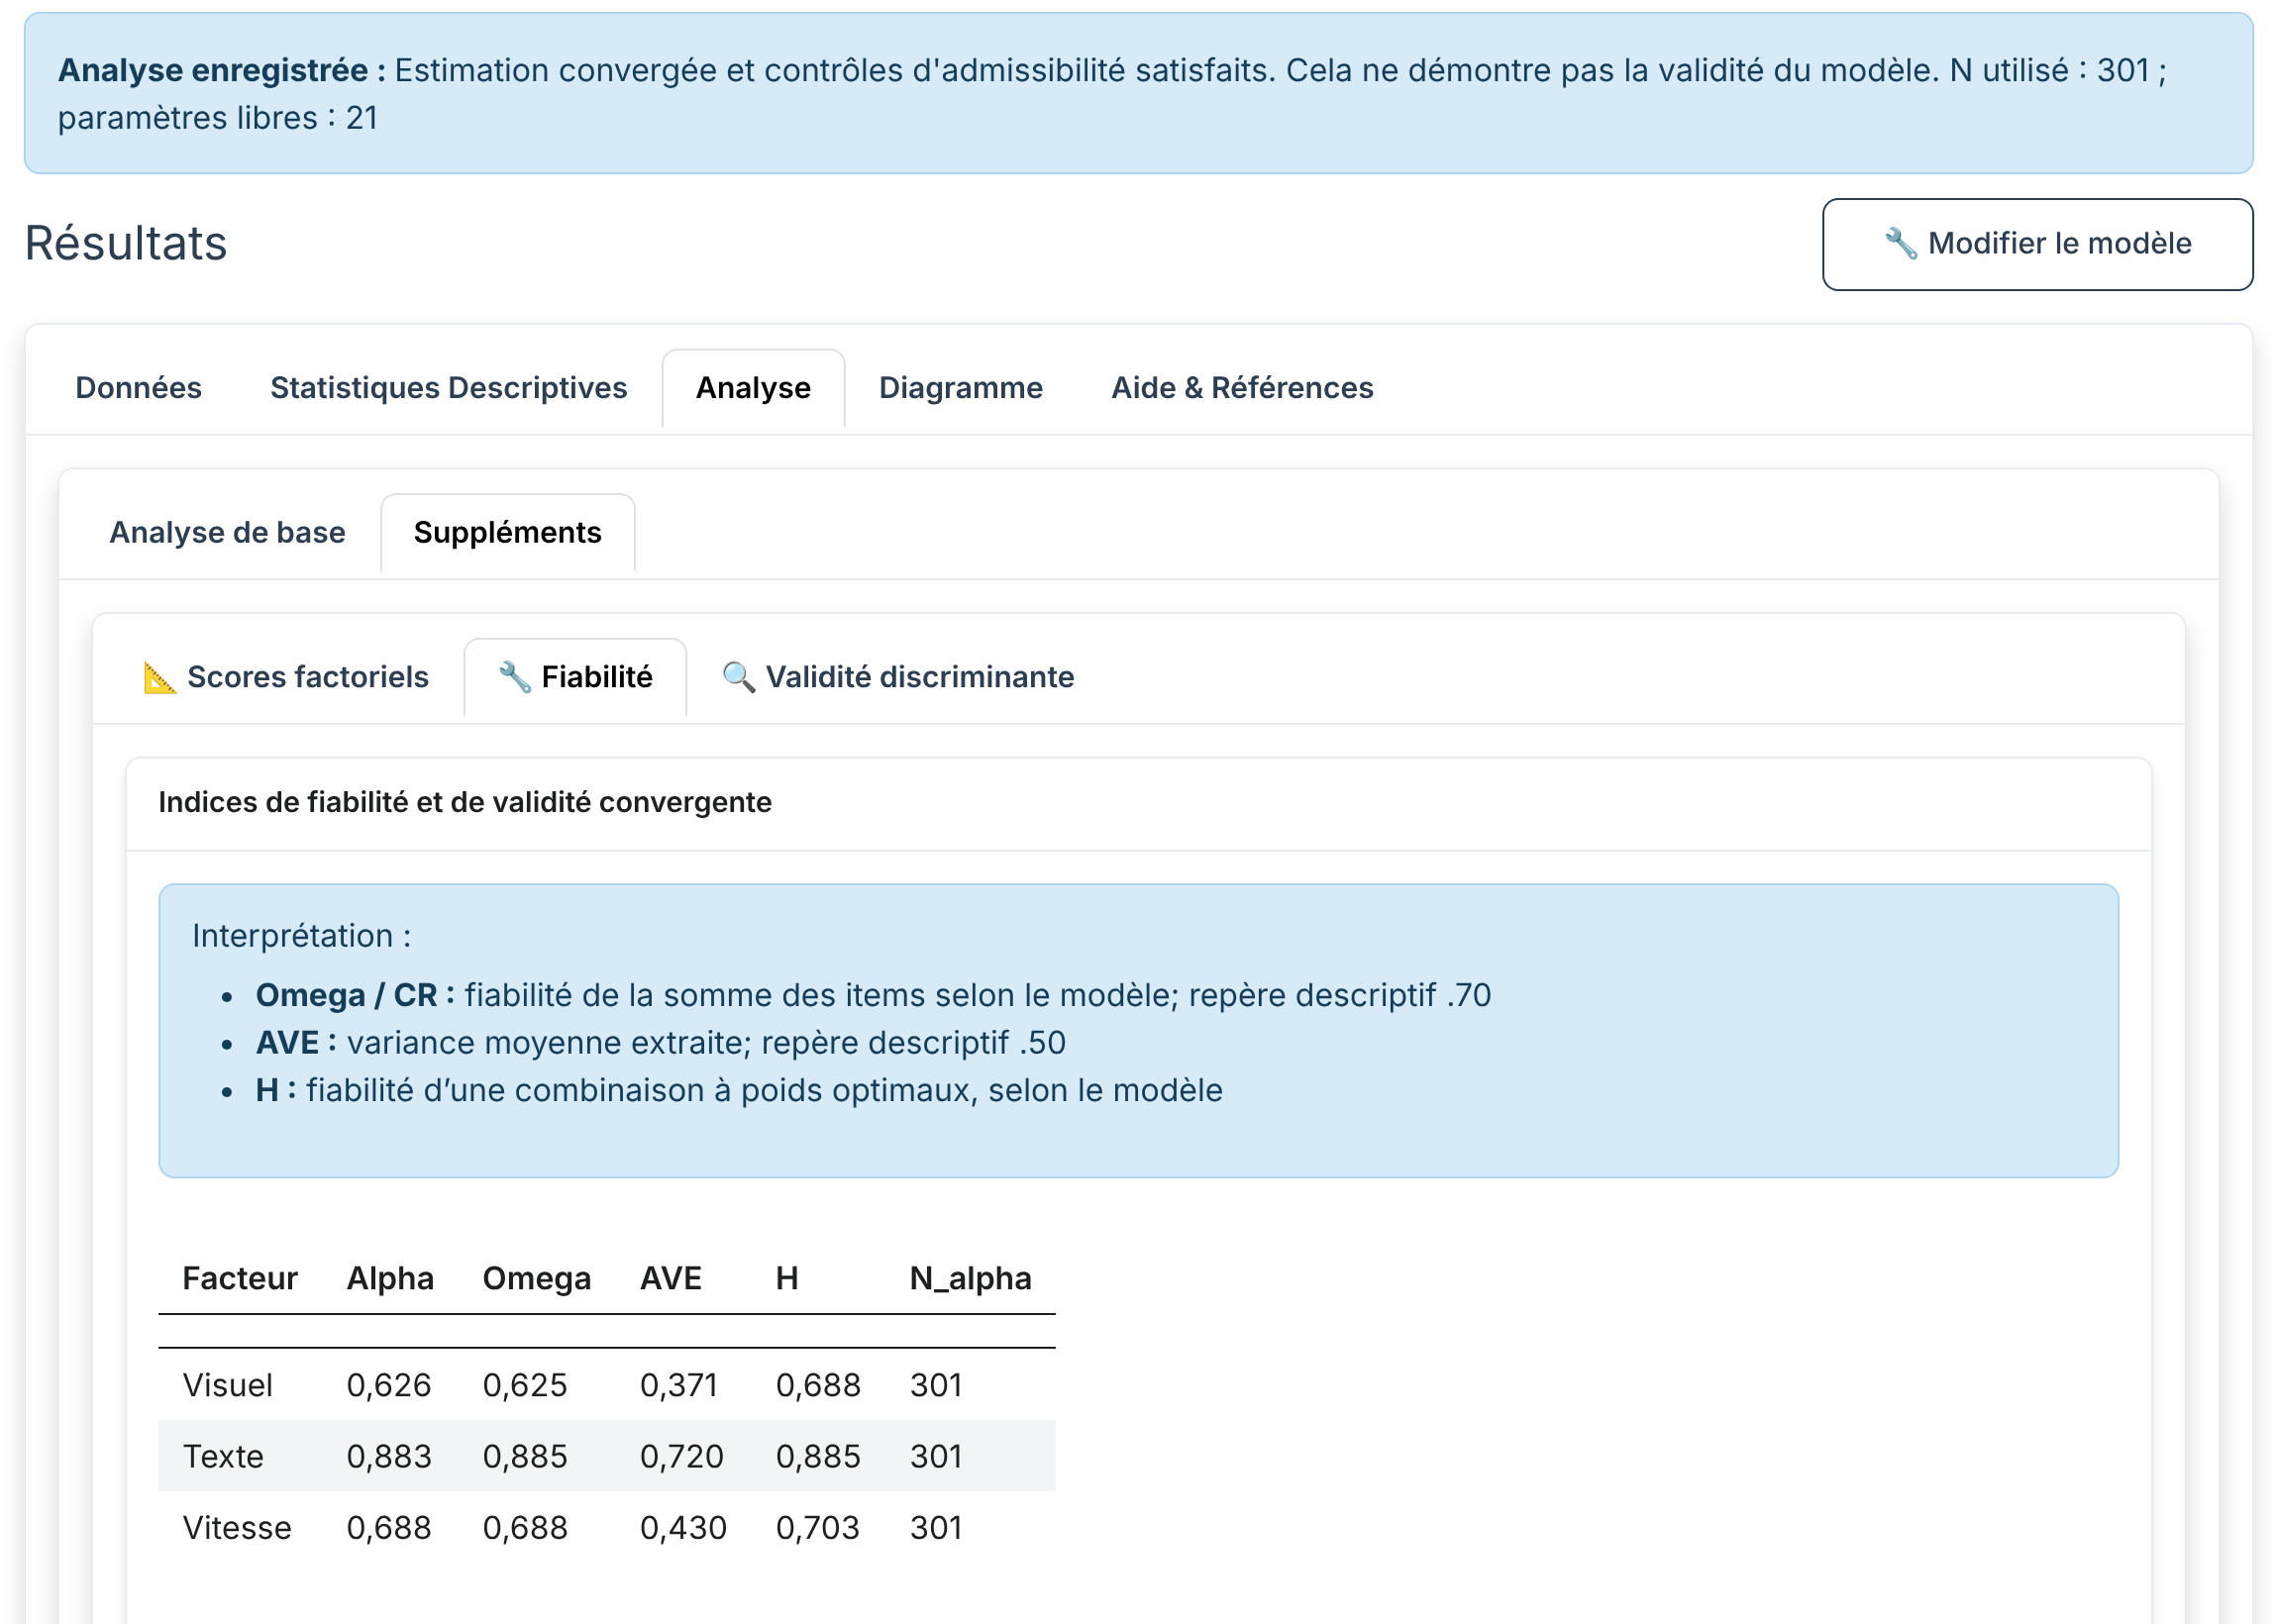
\includegraphics[width=1\linewidth,height=\textheight,keepaspectratio]{images/app/ch06_fiabilite.png}

}

\caption{\label{fig-app-fiabilite}\textbf{Suppléments → Fiabilité} sur
le modèle de référence. L'encadré rappelle la cible de chaque indice; la
colonne N\_alpha donne les cas complets utilisés par alpha.}

\end{figure}%

Voici les repères pour cette analyse :

\Needspace{7\baselineskip}

{

\begin{longtable}[]{@{}lrrrrr@{}}

\caption{\label{tbl-hs-fiab}Indices de fiabilité et de validité
convergente du modèle de référence (moteur de l'application). Omega et
CR désignent la même quantité.}

\tabularnewline

\toprule\noalign{}
Facteur & Alpha & Omega & AVE & H & N\_alpha \\
\midrule\noalign{}
\endhead
\bottomrule\noalign{}
\endlastfoot
Visuel & 0,626 & 0,625 & 0,371 & 0,688 & 301 \\
Texte & 0,883 & 0,885 & 0,720 & 0,885 & 301 \\
Vitesse & 0,688 & 0,688 & 0,430 & 0,703 & 301 \\

\end{longtable}

}

\begin{figure}[htbp]

\centering{

\includegraphics[width=0.88\linewidth,height=\textheight,keepaspectratio]{06-fiabilite_files/figure-pdf/fig-hs-fiab-1.png}

}

\caption{\label{fig-hs-fiab}Alpha, oméga et H par facteur, avec le
repère descriptif de 0,70. L'écart entre H et oméga est le plus grand
pour le facteur visuel, dont les indicateurs contribuent le plus
inégalement.}

\end{figure}%

Le facteur verbal (\texttt{Texte}) est mesuré plus fortement et plus
régulièrement que le facteur visuel dans cette spécification : oméga
0,885 contre 0,625. La fiabilité de la somme des trois indicateurs
visuels reste modeste. Cette observation peut refléter les propriétés
des tests, leur nombre et les limites du modèle.

\section{Alpha}\label{alpha}

Alpha est calculé sur les scores observés. Il dépend des covariances
entre items et de leur nombre. Sa lecture comme fiabilité d'un score
requiert des hypothèses; il n'établit pas que tous les indicateurs
mesurent une seule dimension.

L'application indique \textbf{N\_alpha}, le nombre de cas complets pour
les indicateurs du facteur considéré. Il peut différer entre facteurs et
de l'effectif d'une estimation FIML. Une comparaison entre alpha et
oméga doit donc tenir compte à la fois de leur définition et des
observations utilisées.

Une grande quantité d'items très redondants peut augmenter alpha sans
améliorer proportionnellement la couverture du construit. Inversement,
un petit ensemble couvrant des contenus complémentaires peut avoir une
valeur plus faible. La décision de retenir un score ne se réduit pas à
maximiser cet indice.

\section{Oméga et CR}\label{omuxe9ga-et-cr}

Dans cette application, \textbf{Omega} et \textbf{CR} désignent la même
quantité calculée pour la somme des indicateurs, dans leurs unités
d'origine, selon le modèle. Ce ne sont pas deux preuves indépendantes.

Pour un facteur de variance \(\phi\), des saturations
\(\boldsymbol{\lambda}\) et une matrice résiduelle \(\Theta\), la
formule utilisée est :

\[\omega=\frac{\phi(\sum_i\lambda_i)^2}{\phi(\sum_i\lambda_i)^2+\boldsymbol{1}^{\mathsf T}\Theta\boldsymbol{1}}.\]

La matrice résiduelle complète intervient au dénominateur. Une
covariance résiduelle peut donc modifier la fiabilité de la somme; elle
ne doit pas disparaître d'un calcul simplifié. La variance totale au
dénominateur est celle reproduite par le modèle pour ce score.

L'effet est net sur HS. Si l'on ajoute la covariance résiduelle entre
\texttt{x7} et \texttt{x8} suggérée au chapitre précédent, l'oméga du
facteur vitesse passe de 0,688 à 0,559, alors qu'alpha, calculé sur les
seules covariances observées, ne bouge pas (0,688). Une partie de ce que
\texttt{x7} et \texttt{x8} partagent est désormais attribuée à leur lien
propre plutôt qu'au facteur : la somme des trois tests mesure moins bien
la vitesse qu'on ne le croyait. H, lui, monte à 0,916, parce qu'une
pondération optimale peut exploiter la structure des erreurs; ce score
pondéré s'éloigne alors de la somme qu'on utilisera.

Cette formule suppose que le score visé est effectivement la somme des
items dans le codage analysé. Si certaines saturations sont négatives
parce que des items sont orientés en sens inverse, leur compensation
peut réduire fortement la composante commune de la somme. Ce n'est pas
une anomalie à masquer en prenant toutes les saturations en valeur
absolue.

\section{H}\label{h}

\textbf{H} décrit une combinaison à poids optimaux selon le modèle
(\citeproc{ref-hancock2001}{Hancock et Mueller 2001}). Sa cible est
différente de celle d'une somme à poids égaux. Une valeur de H
supérieure à celle d'oméga n'implique pas que la somme utilisée dans
votre recherche possède cette fiabilité plus élevée.

Dans le modèle simple, le calcul peut s'écrire \(H=a/(1+a)\), où
\(a=\phi\boldsymbol{\lambda}^{\mathsf T}\Theta^{-1}\boldsymbol{\lambda}\).
Cette écriture explique pourquoi la covariance résiduelle et la qualité
respective des indicateurs interviennent. Elle n'impose pas de calcul
manuel au lecteur.

Sur HS, la différence entre H et oméga est plus visible pour le facteur
visuel (0,688 contre 0,625) que pour le facteur verbal (0,885 contre
0,885). Les indicateurs visuels ne contribuent pas tous avec la même
qualité : un score qui donnerait plus de poids à \texttt{x1} et moins à
\texttt{x2} serait plus fiable que leur somme. Mentionnez la cible du
coefficient avant de comparer leurs valeurs.

\section{AVE}\label{ave}

La \textbf{variance moyenne extraite}, ou AVE, résume la proportion de
variance des indicateurs attribuée au facteur. Dans une structure
simple, elle est la moyenne des saturations entièrement standardisées au
carré (\citeproc{ref-fornell1981}{Fornell et Larcker 1981}). Elle ne
doit pas être lue comme le coefficient de fiabilité de la somme.

L'AVE du facteur verbal (0,720) est nettement supérieure à celle du
facteur visuel (0,371). L'interprétation est cohérente avec les
saturations déjà observées. Le repère 0,50 exprime l'idée que le facteur
explique en moyenne une part substantielle de la variance de ses
indicateurs; il n'est pas une preuve autonome de validité convergente.
Une AVE inférieure à 0,50 avec un oméga acceptable n'a rien de
contradictoire : chaque indicateur est imparfait, mais leur somme l'est
moins.

\section{Les repères ne remplacent pas l'usage
visé}\label{les-repuxe8res-ne-remplacent-pas-lusage-visuxe9}

On rencontre souvent 0,70 pour la fiabilité et 0,50 pour l'AVE. Ces
valeurs peuvent servir de points de discussion. Elles ne déterminent pas
seules si un score convient à une comparaison de groupes, à une
exploration pédagogique ou à une décision individuelle à enjeu
important.

Examinez le contenu des items, la précision nécessaire, le nombre
d'indicateurs, les erreurs-types disponibles et la stabilité dans
d'autres échantillons. Un coefficient unique n'épuise pas la qualité
d'un instrument.

\section{Attention aux items inversés du
BFI}\label{attention-aux-items-inversuxe9s-du-bfi}

Le fichier BFI de l'application conserve le codage original. Les clés
identifient notamment A1, C4, C5, E1, E2, O2 et O5 comme orientés en
sens inverse. Une saturation négative peut être cohérente avec ce
codage. Elle ne signifie pas automatiquement que l'item est mauvais.
Dans le modèle préparé, 11 saturations sont négatives : A2, A3, A4, A5,
C4, C5, E3, E4, E5, O2, O5. Cette liste ne coïncide pas avec celle des
items inversés, et c'est normal : avec \textbf{λ₁=1}, chaque facteur
prend l'orientation de son premier item. Quand ce premier item est
lui-même inversé (A1, E1), ce sont les items directs qui apparaissent
négatifs. Le signe d'une saturation se lit donc toujours par rapport à
l'item de référence.

\Needspace{9\baselineskip}

{

\begin{longtable}[]{@{}lrrrr@{}}

\caption{\label{tbl-bfi-fiab}BFI / SAPA, codage d'origine (WLSMV, 2\,436
cas complets). Alpha porte sur la somme des réponses observées; oméga, H
et AVE portent sur les réponses latentes.}

\tabularnewline

\toprule\noalign{}
Facteur & Alpha & Omega & AVE & H \\
\midrule\noalign{}
\endhead
\bottomrule\noalign{}
\endlastfoot
Agreabilite & 0,444 & 0,673 & 0,423 & 0,820 \\
Conscience & −0,316 & 0,026 & 0,418 & 0,796 \\
Extraversion & −0,655 & 0,181 & 0,449 & 0,813 \\
Neuroticisme & 0,817 & 0,860 & 0,556 & 0,885 \\
Ouverture & −0,176 & 0,135 & 0,311 & 0,775 \\

\end{longtable}

}

\begin{figure}[htbp]

\centering{

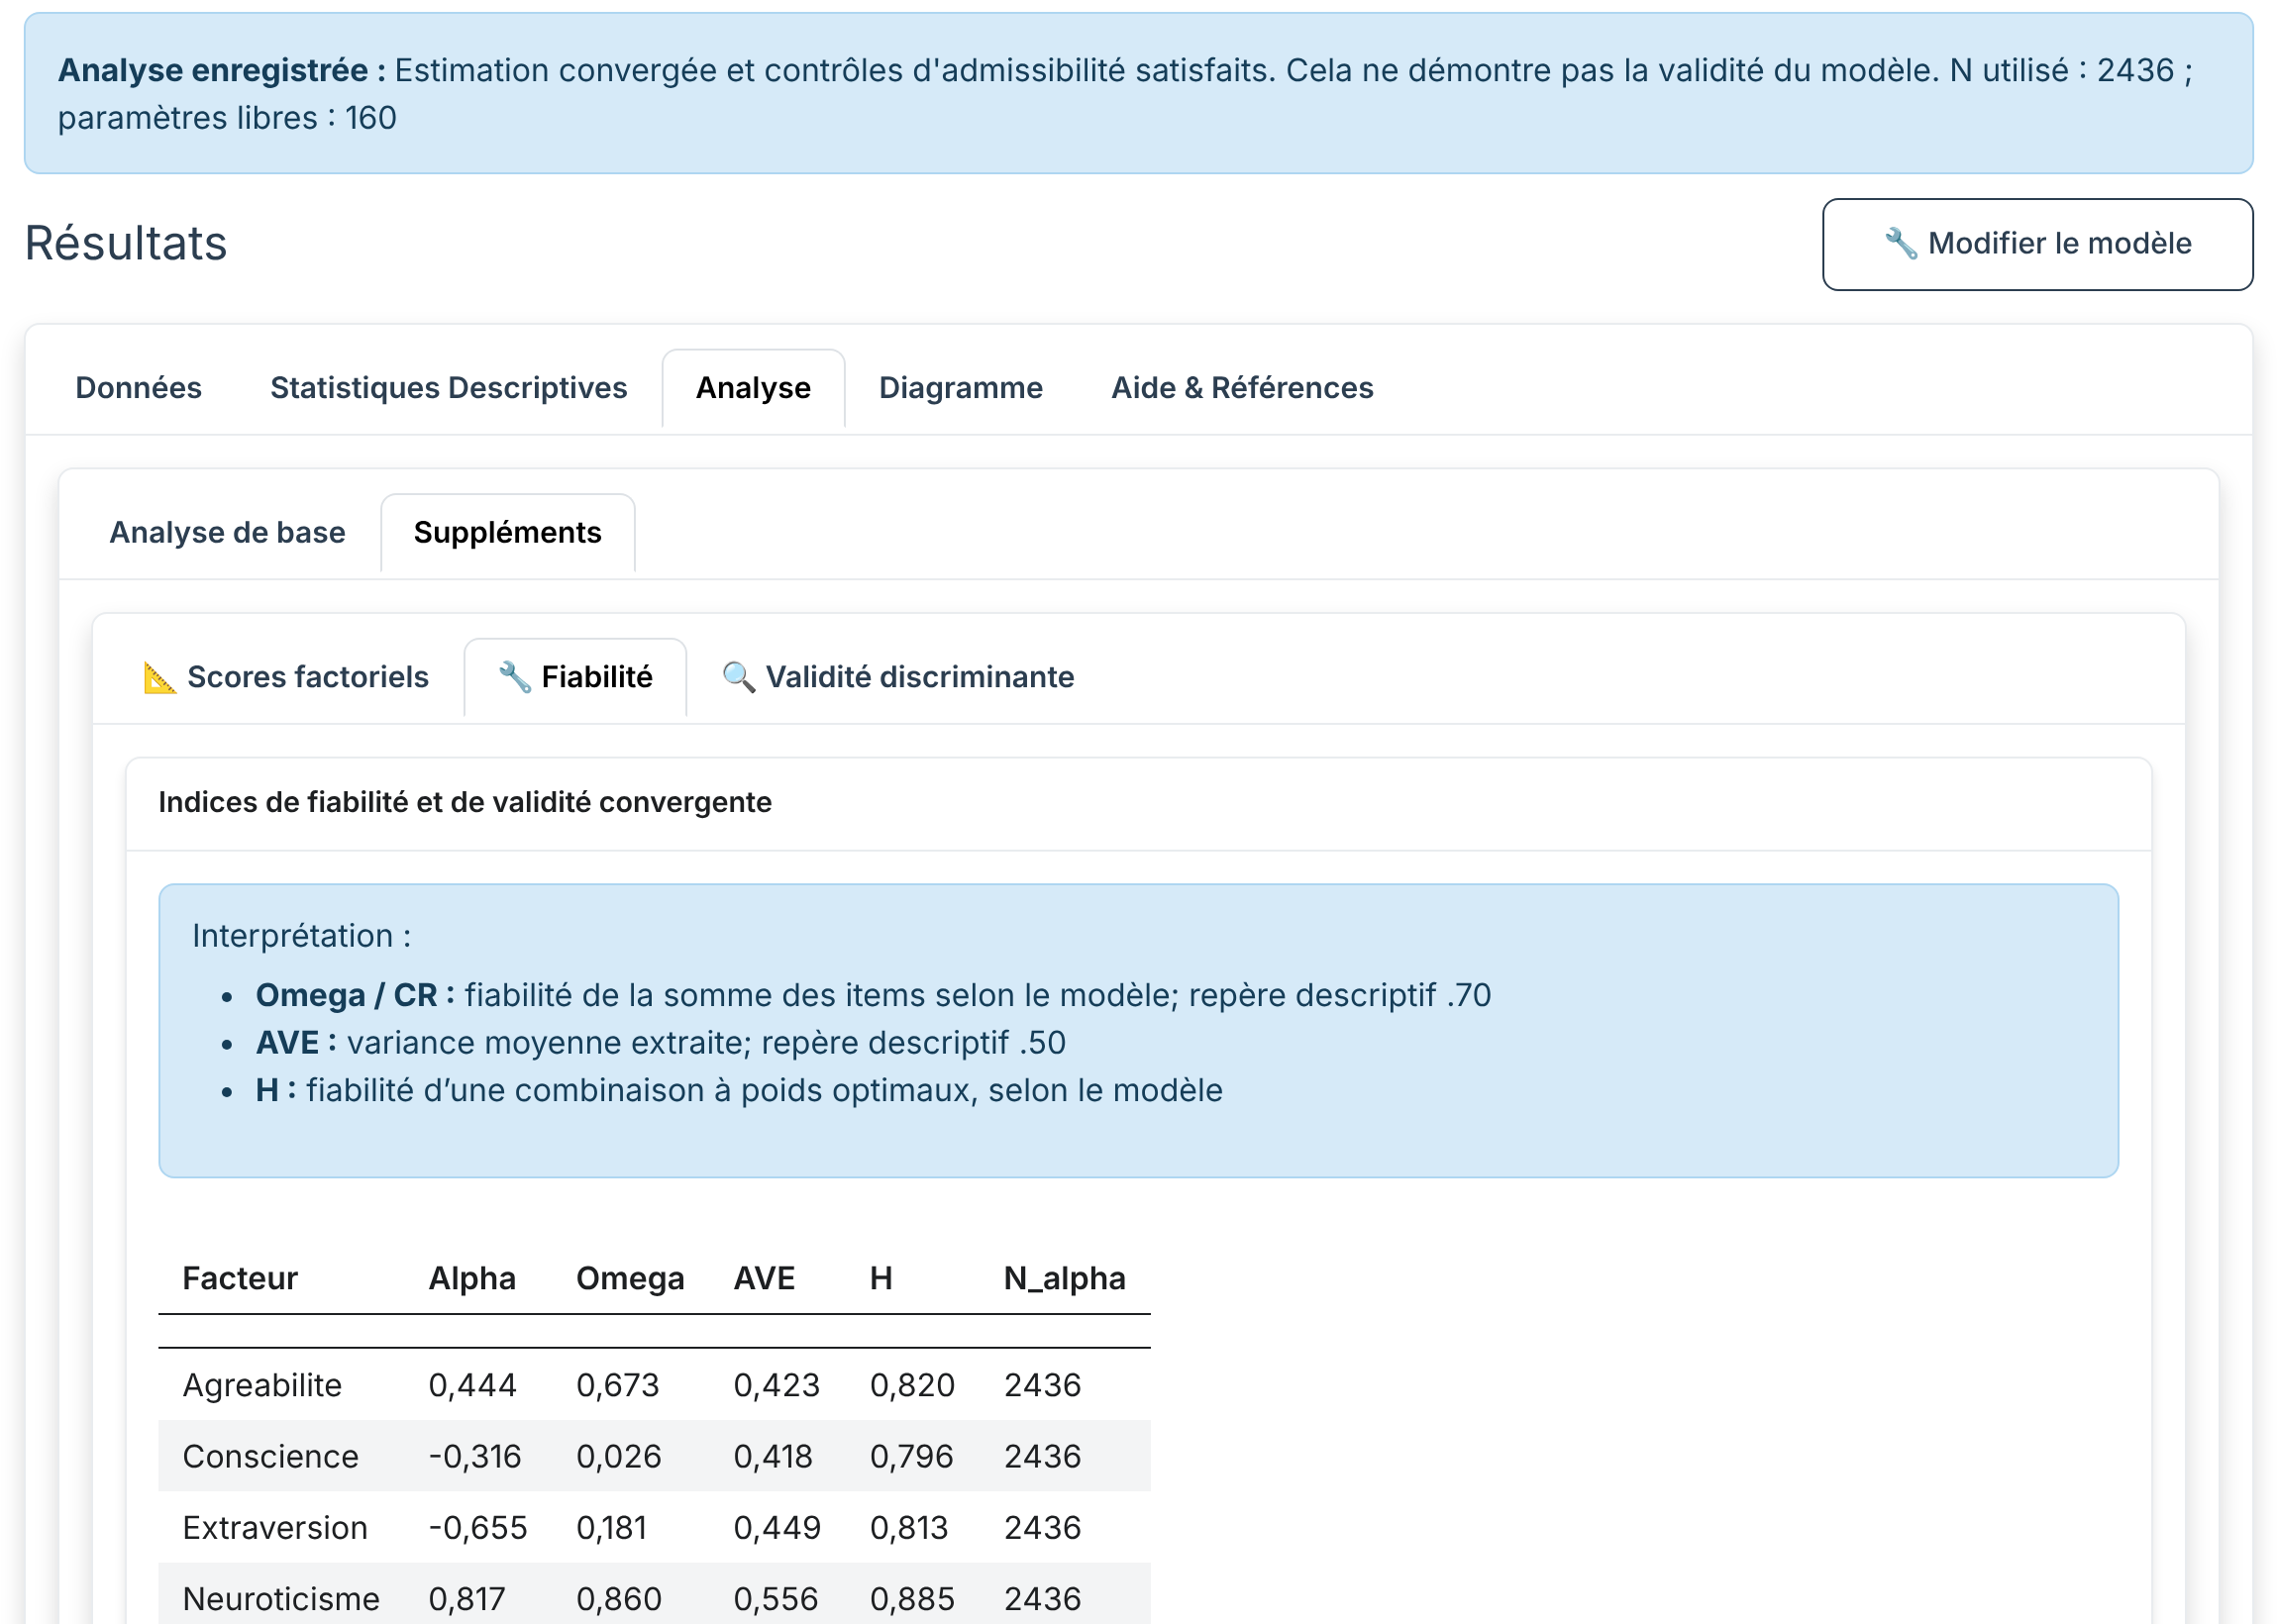
\includegraphics[width=1\linewidth,height=\textheight,keepaspectratio]{images/app/ch06_fiabilite_bfi.png}

}

\caption{\label{fig-app-fiab-bfi}\textbf{Fiabilité} sur le BFI non
recodé : alphas négatifs pour trois facteurs, oméga très faible, mais H
élevé.}

\end{figure}%

Le contraste est spectaculaire pour le facteur \texttt{Conscience} :
alpha vaut −0,316 et oméga 0,026, alors que H atteint 0,796. La somme
brute additionne des items de sens opposés, qui s'annulent en partie; la
combinaison optimale de H, elle, donne un poids négatif aux items
inversés. Seuls \texttt{Neuroticisme}, dont aucun item n'est inversé, et
dans une moindre mesure \texttt{Agreabilite}, gardent une somme brute
interprétable.

Avant de calculer une somme orientée dans une direction commune, il
faudrait recoder les items concernés selon une règle explicite, puis
réestimer et documenter l'analyse. Pour une échelle allant de 1 à 6,
l'inversion usuelle est \(7-X\). Cette opération modifie le score
défini. L'application ne l'accomplit pas silencieusement à votre place.

\section{Avec des indicateurs
ordinaux}\label{avec-des-indicateurs-ordinaux}

Dans les analyses ordinales de cette application, oméga, CR, H et AVE
portent sur les \textbf{réponses latentes continues} qui sous-tendent
les catégories. Alpha porte sur les scores observés. Les différences
entre ces coefficients ne sont donc pas seulement des différences de
méthodes de calcul sur une même cible.

Vous ne pouvez pas affirmer que la somme observée de dix catégories
possède une fiabilité de 0,94 uniquement parce que l'oméga de la réponse
latente vaut 0,94. Le chapitre sur les données ordinales reviendra sur
cette distinction. Conservez-la déjà lorsque vous lisez les tableaux du
MSQ ou du BFI.

\section{Laboratoire : quatre phrases sur une même
analyse}\label{laboratoire-quatre-phrases-sur-une-muxeame-analyse}

À partir du tableau HS, rédigez quatre phrases : une sur la somme des
indicateurs visuels, une sur le facteur verbal, une distinguant H
d'oméga et une précisant pourquoi la convergence n'établit pas la
fiabilité. Évitez d'additionner les arguments Omega et CR comme s'ils
constituaient deux observations séparées.

\begin{tcolorbox}[enhanced jigsaw, arc=.35mm, bottomrule=.15mm, bottomtitle=1mm, breakable, colback=white, colbacktitle=quarto-callout-tip-color!10!white, colframe=quarto-callout-tip-color-frame, coltitle=black, left=2mm, leftrule=.75mm, opacityback=0, opacitybacktitle=0.6, rightrule=.15mm, title={Réponse}, titlerule=0mm, toprule=.15mm, toptitle=1mm]

\begin{enumerate}
\def\labelenumi{\arabic{enumi}.}
\tightlist
\item
  « La somme des trois tests visuels a une fiabilité modeste selon le
  modèle (oméga = 0,625), sous le repère usuel de 0,70. »
\item
  « Les trois tests verbaux forment un score fiable (oméga = 0,885; AVE
  = 0,720). »
\item
  « Pour le facteur visuel, H (0,688) dépasse oméga : une pondération
  qui favoriserait \texttt{x1} améliorerait la fiabilité, mais ce ne
  serait plus la somme simple. »
\item
  « Une estimation convergée et admissible permet de calculer ces
  indices; elle ne dit pas si les scores sont assez fiables pour l'usage
  visé. »
\end{enumerate}

\end{tcolorbox}

\begin{tcolorbox}[enhanced jigsaw, arc=.35mm, bottomrule=.15mm, bottomtitle=1mm, breakable, colback=white, colbacktitle=quarto-callout-important-color!10!white, colframe=quarto-callout-important-color-frame, coltitle=black, left=2mm, leftrule=.75mm, opacityback=0, opacitybacktitle=0.6, rightrule=.15mm, title={À retenir}, titlerule=0mm, toprule=.15mm, toptitle=1mm]

\begin{itemize}
\tightlist
\item
  Dire de quel score on parle avant de citer une fiabilité.
\item
  Oméga et CR sont ici la même quantité; alpha porte sur les données,
  oméga et H sur le modèle.
\item
  Une covariance résiduelle diminue l'oméga de la somme et peut gonfler
  H.
\item
  Des items inversés non recodés peuvent ruiner la fiabilité d'une somme
  brute sans affaiblir le facteur.
\end{itemize}

\end{tcolorbox}

\section{Quiz}\label{quiz-5}

\begin{enumerate}
\def\labelenumi{\arabic{enumi}.}
\tightlist
\item
  Alpha et oméga sont presque égaux pour le facteur \texttt{Texte}.
  Qu'est-ce que cela suggère sur ses indicateurs ?
\item
  Peut-on citer H pour décrire la fiabilité de la moyenne des items
  d'une échelle ?
\item
  L'AVE du facteur \texttt{Vitesse} vaut 0,430. Ses indicateurs sont-ils
  inutilisables ?
\item
  Pourquoi un alpha négatif ne doit-il pas être ramené à zéro ?
\end{enumerate}

\begin{tcolorbox}[enhanced jigsaw, arc=.35mm, bottomrule=.15mm, bottomtitle=1mm, breakable, colback=white, colbacktitle=quarto-callout-tip-color!10!white, colframe=quarto-callout-tip-color-frame, coltitle=black, left=2mm, leftrule=.75mm, opacityback=0, opacitybacktitle=0.6, rightrule=.15mm, title={Réponses}, titlerule=0mm, toprule=.15mm, toptitle=1mm]

\begin{enumerate}
\def\labelenumi{\arabic{enumi}.}
\tightlist
\item
  Que les trois tests contribuent de façon semblable au facteur :
  l'hypothèse de contributions égales d'alpha est alors peu violée.
\item
  Non. H décrit une combinaison pondérée de façon optimale, pas une
  moyenne à poids égaux.
\item
  Non. Chaque test garde une part substantielle de variance propre, mais
  leur somme a un oméga de 0,688. L'AVE décrit les indicateurs un à un.
\item
  Il signale que la somme brute n'a pas de cohérence interprétable,
  souvent à cause d'items inversés; le masquer cacherait un problème de
  définition du score.
\end{enumerate}

\end{tcolorbox}

\bookmarksetup{startatroot}

\chapter{Examiner la distinction entre les facteurs}\label{sec-validite}

\begin{tcolorbox}[enhanced jigsaw, arc=.35mm, bottomrule=.15mm, bottomtitle=1mm, breakable, colback=white, colbacktitle=quarto-callout-note-color!10!white, colframe=quarto-callout-note-color-frame, coltitle=black, left=2mm, leftrule=.75mm, opacityback=0, opacitybacktitle=0.6, rightrule=.15mm, title={Objectifs du chapitre}, titlerule=0mm, toprule=.15mm, toptitle=1mm]

\begin{itemize}
\tightlist
\item
  Lire les corrélations entre facteurs, le critère de Fornell et
  Larcker, le HTMT et le HTMT2.
\item
  Comprendre ce que chaque critère compare et sur quelle matrice il est
  calculé.
\item
  Ajouter une information d'incertitude par bootstrap.
\item
  Formuler une conclusion prudente sur la distinction des construits.
\end{itemize}

\end{tcolorbox}

\begin{tcolorbox}[enhanced jigsaw, arc=.35mm, bottomrule=.15mm, bottomtitle=1mm, breakable, colback=white, colbacktitle=quarto-callout-tip-color!10!white, colframe=quarto-callout-tip-color-frame, coltitle=black, left=2mm, leftrule=.75mm, opacityback=0, opacitybacktitle=0.6, rightrule=.15mm, title={Idée centrale}, titlerule=0mm, toprule=.15mm, toptitle=1mm]

Deux facteurs liés peuvent rester distincts. Les critères de validité
discriminante comparent, chacun à sa façon, ce que les indicateurs d'un
facteur partagent entre eux et ce qu'ils partagent avec ceux d'un autre
facteur. Ils renseignent sur la séparation empirique; le sens des
construits reste une question de contenu.

\end{tcolorbox}

\section{Des facteurs liés peuvent rester
distincts}\label{des-facteurs-liuxe9s-peuvent-rester-distincts}

Deux construits peuvent être fortement associés sans être
interchangeables. L'AFC à facteurs corrélés permet d'examiner cette
possibilité. Mais une étiquette différente sur chaque cercle du
diagramme ne suffit pas à établir que les dimensions sont empiriquement
distinguables.

La validité discriminante demande une lecture des corrélations
factorielles, des relations entre items, de leur contenu et de
l'incertitude. Les indices présentés ici sont des éléments du
raisonnement. Ils ne remplacent pas l'examen conceptuel des construits.

\section{Corrélations factorielles}\label{corruxe9lations-factorielles}

Commencez par les corrélations estimées entre facteurs. Une valeur
proche de 1 en valeur absolue appelle une attention particulière. Une
valeur hors de l'intervalle admissible, une matrice factorielle
problématique ou une solution inadmissible empêchent une lecture
ordinaire de ces coefficients.

Ne confondez pas une covariance avec une corrélation. La première dépend
des échelles factorielles; la seconde exprime une relation standardisée.
Une covariance plus grande après changement d'identification ne signifie
pas nécessairement un lien substantiel plus fort.

Dans HS, les corrélations entre les trois facteurs vont de 0,283 à
0,471, sans être imposées parfaites. Leur sens est cohérent avec des
aptitudes cognitives associées. La question reste de savoir si leurs
indicateurs permettent de défendre les distinctions proposées.

\section{Le tableau AVE de Fornell et
Larcker}\label{le-tableau-ave-de-fornell-et-larcker}

Ouvrez \textbf{Analyse → Suppléments → Validité discriminante}. La
diagonale du premier tableau contient les racines carrées des AVE. Les
valeurs hors diagonale sont les corrélations factorielles. Le critère
compare la racine carrée de l'AVE aux corrélations correspondantes en
\textbf{valeur absolue} (\citeproc{ref-fornell1981}{Fornell et Larcker
1981}).

\Needspace{7\baselineskip}

{

\begin{longtable}[]{@{}lrrr@{}}

\caption{\label{tbl-fl}Critère de Fornell et Larcker pour le modèle de
référence : racine carrée de l'AVE sur la diagonale, corrélations entre
facteurs sous la diagonale.}

\tabularnewline

\toprule\noalign{}
Facteur & Visuel & Texte & Vitesse \\
\midrule\noalign{}
\endhead
\bottomrule\noalign{}
\endlastfoot
Visuel & 0,609 & & \\
Texte & 0,459 & 0,848 & \\
Vitesse & 0,471 & 0,283 & 0,656 \\

\end{longtable}

}

\begin{figure}[htbp]

\centering{

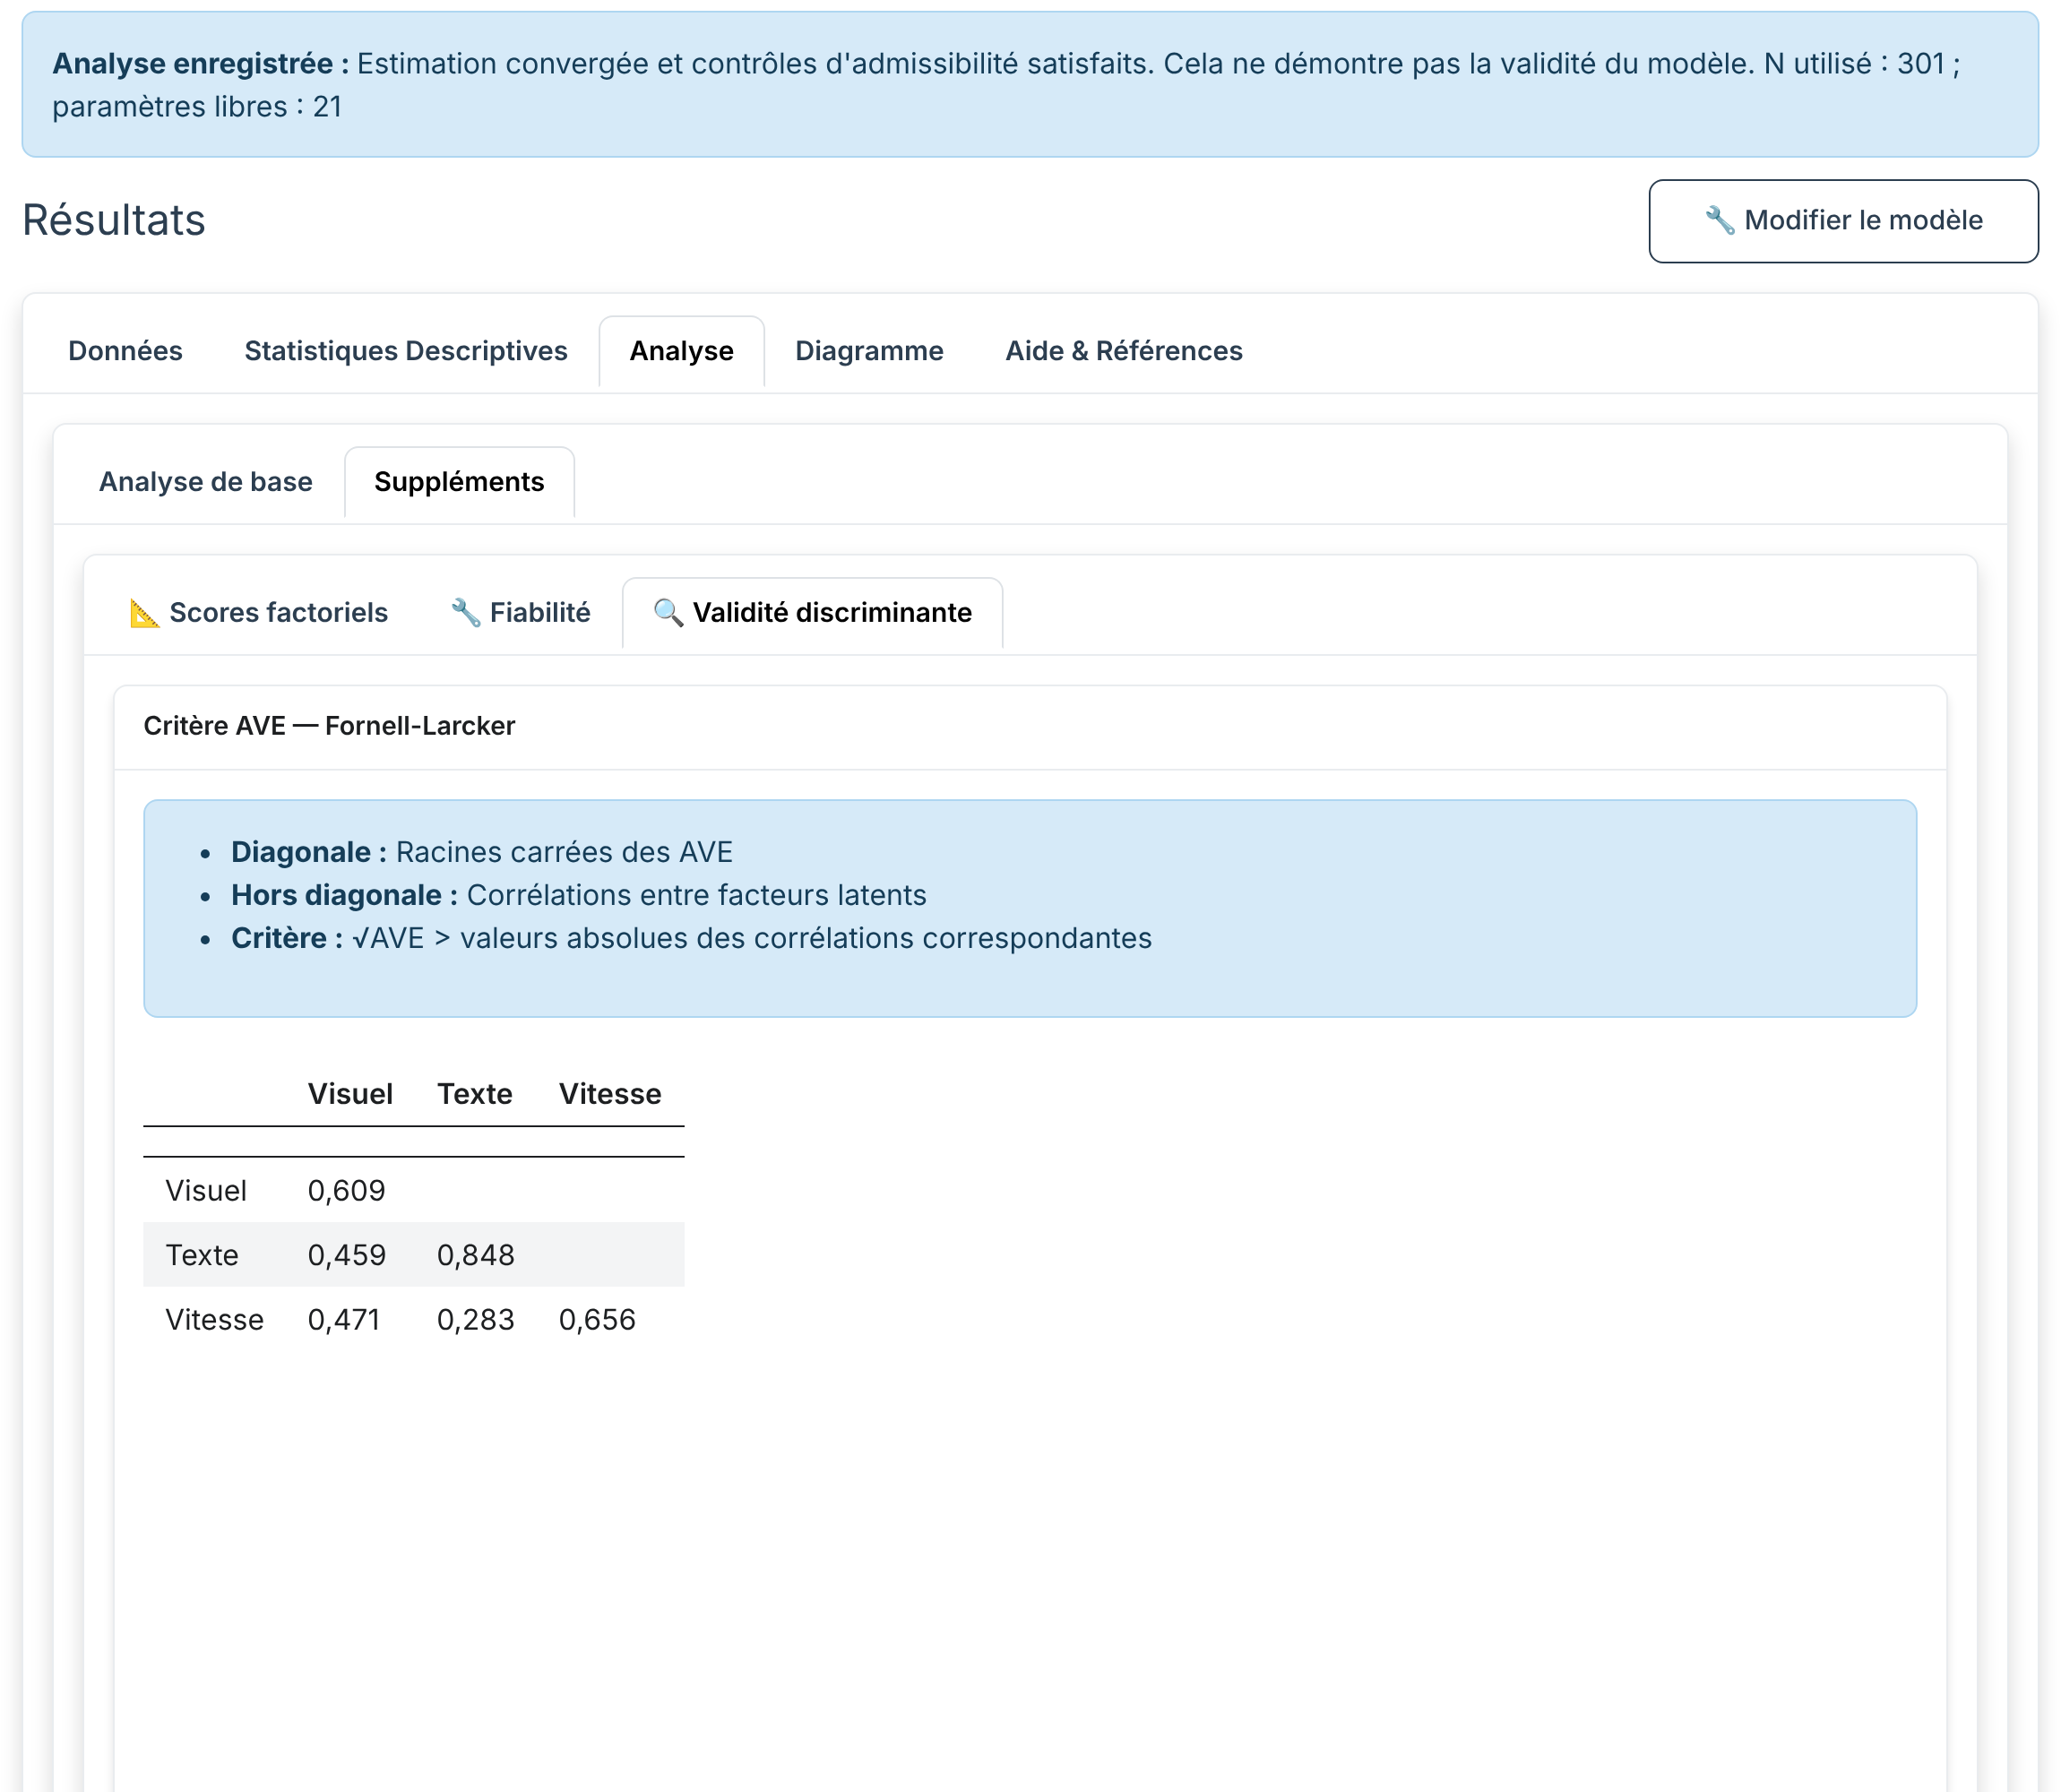
\includegraphics[width=1\linewidth,height=\textheight,keepaspectratio]{images/app/ch07_validite.png}

}

\caption{\label{fig-app-validite}\textbf{Suppléments → Validité
discriminante} : l'encadré rappelle la lecture du tableau de Fornell et
Larcker; le tableau du HTMT suit plus bas dans le même onglet.}

\end{figure}%

Chaque racine d'AVE dépasse ici les corrélations de sa ligne et de sa
colonne : par exemple, pour \texttt{Visuel}, 0,609 contre 0,459 et
0,471. Ce critère équivaut à demander que l'AVE dépasse la MSV, le plus
grand carré des corrélations du facteur (colonnes \textbf{MSV} et
\textbf{ASV} du tableau de fiabilité).

Par exemple, une corrélation de −0,80 est plus forte en valeur absolue
qu'une racine d'AVE de 0,70; le signe négatif ne rend pas le critère
favorable. La comparaison doit être faite pour chacun des deux facteurs
d'une paire.

Un critère satisfait ne démontre pas à lui seul la validité
discriminante. Il synthétise un aspect de la relation entre variance
extraite et chevauchement des facteurs. Il est aussi très exigeant
lorsque les saturations sont modérées : avec une AVE de 0,30, une
corrélation de 0,55 entre facteurs suffit à le faire échouer.

\section{HTMT}\label{htmt}

Le \textbf{HTMT} compare l'intensité des corrélations entre indicateurs
de facteurs différents à celle des corrélations entre indicateurs d'un
même facteur. Il est calculé ici à partir des corrélations des données
utilisées par l'estimation, et non à partir d'une matrice de
corrélations reproduite par le modèle : c'est ce qui en fait un contrôle
indépendant de l'estimation.

\[\text{HTMT}_{ij}=\frac{\bar r_{ij}}{\sqrt{\bar r_{ii}\,\bar r_{jj}}}\]

Le numérateur est la moyenne des corrélations entre un indicateur de
\(i\) et un indicateur de \(j\); le dénominateur est la moyenne
géométrique des corrélations moyennes entre indicateurs distincts d'un
même facteur. L'application utilise les valeurs absolues des
corrélations. Les repères 0,85 et 0,90 sont affichés comme points de
lecture, plus ou moins exigeants. Ils ne font pas disparaître
l'incertitude d'échantillonnage et ne constituent pas un verdict
universel (\citeproc{ref-henseler2015}{Henseler et al. 2015}).

Pour le modèle HS de référence :

\Needspace{7\baselineskip}

{

\begin{longtable}[]{@{}lrrr@{}}

\caption{\label{tbl-htmt}Corrélations entre facteurs, HTMT et HTMT2 du
modèle de référence.}

\tabularnewline

\toprule\noalign{}
Paire & Corrélation factorielle & HTMT & HTMT2 \\
\midrule\noalign{}
\endhead
\bottomrule\noalign{}
\endlastfoot
Visuel -- Texte & 0,459 & 0,424 & 0,384 \\
Visuel -- Vitesse & 0,471 & 0,467 & 0,387 \\
Texte -- Vitesse & 0,283 & 0,290 & 0,280 \\

\end{longtable}

}

\begin{figure}[htbp]

\centering{

\includegraphics[width=0.88\linewidth,height=\textheight,keepaspectratio]{07-validite_files/figure-pdf/fig-htmt-1.png}

}

\caption{\label{fig-htmt}Corrélation entre facteurs, HTMT et HTMT2 pour
les trois paires de HS. Les trois lectures restent loin du repère de
0,85 (ligne pointillée). Elles ne coïncident pas : le HTMT voit les
données telles qu'elles sont, la corrélation factorielle passe par le
modèle.}

\end{figure}%

Comparez ces valeurs aux corrélations factorielles, sans exiger qu'elles
leur soient exactement égales. Les deux calculs utilisent des
informations liées, mais leur construction diffère. Une valeur élevée
doit conduire à examiner le contenu partagé, la qualité des indicateurs
et les autres diagnostics.

Avec un seul facteur, il n'existe aucune paire de facteurs dont on
pourrait examiner la distinction. L'absence de HTMT dans ce cas est
attendue; ce n'est pas un échec de l'analyse.

\section{HTMT2}\label{htmt2}

Le complément \textbf{HTMT2} est accessible en \textbf{Options
avancées}, dans \textbf{4. Interpréter}. Il remplace les moyennes
arithmétiques par des moyennes géométriques. Lorsque les saturations
d'un même facteur sont inégales, le HTMT s'écarte de la corrélation
vraie entre facteurs; le HTMT2 est conçu pour la retrouver dans ce cas.
Il demeure un indice apparenté au HTMT, pas une validation indépendante
(\citeproc{ref-roemer2021}{Roemer et al. 2021};
\citeproc{ref-semtoolshtmt}{Équipe semTools 2026}).

La présence de corrélations nulles ou non calculables peut rendre
certaines valeurs indisponibles. Une case manquante doit être comprise à
partir de cette définition, et non remplacée par zéro. Des indicateurs
mal reliés à leur propre facteur peuvent aussi fragiliser la lecture du
rapport de corrélations.

\section{Ajouter une information sur
l'incertitude}\label{ajouter-une-information-sur-lincertitude}

Le panneau avancé permet de demander un intervalle bootstrap du HTMT ou
du HTMT2. Ce calcul n'est pas lancé automatiquement. Choisissez
l'indice, le nombre de réplications et la graine, puis cliquez sur
\textbf{Calculer les intervalles}.

Pour une première utilisation sur HS, demandez \textbf{1 000
réplications} et la \textbf{graine 123}. Lisez l'intervalle percentile
bilatéral à 95 \%, mais aussi le nombre de réplications valides. Un
intervalle large signifie que le point estimé ne décrit pas toute
l'incertitude. Les bornes peuvent varier légèrement si le nombre de
réplications ou l'environnement change.

\Needspace{7\baselineskip}

{

\begin{longtable}[]{@{}
  >{\raggedright\arraybackslash}p{(\linewidth - 12\tabcolsep) * \real{0.1220}}
  >{\raggedright\arraybackslash}p{(\linewidth - 12\tabcolsep) * \real{0.1220}}
  >{\raggedleft\arraybackslash}p{(\linewidth - 12\tabcolsep) * \real{0.0732}}
  >{\raggedleft\arraybackslash}p{(\linewidth - 12\tabcolsep) * \real{0.1585}}
  >{\raggedleft\arraybackslash}p{(\linewidth - 12\tabcolsep) * \real{0.1341}}
  >{\raggedleft\arraybackslash}p{(\linewidth - 12\tabcolsep) * \real{0.1341}}
  >{\raggedleft\arraybackslash}p{(\linewidth - 12\tabcolsep) * \real{0.2561}}@{}}

\caption{\label{tbl-boot}Intervalles bootstrap percentile à 95 \% du
HTMT (1 000 réplications, graine 123), tels que les calcule
l'application.}

\tabularnewline

\toprule\noalign{}
\begin{minipage}[b]{\linewidth}\raggedright
Facteur 1
\end{minipage} & \begin{minipage}[b]{\linewidth}\raggedright
Facteur 2
\end{minipage} & \begin{minipage}[b]{\linewidth}\raggedleft
HTMT
\end{minipage} & \begin{minipage}[b]{\linewidth}\raggedleft
ET bootstrap
\end{minipage} & \begin{minipage}[b]{\linewidth}\raggedleft
Borne inf.
\end{minipage} & \begin{minipage}[b]{\linewidth}\raggedleft
Borne sup.
\end{minipage} & \begin{minipage}[b]{\linewidth}\raggedleft
Réplications valides
\end{minipage} \\
\midrule\noalign{}
\endhead
\bottomrule\noalign{}
\endlastfoot
Visuel & Texte & 0,424 & 0,073 & 0,288 & 0,565 & 1\,000 \\
Visuel & Vitesse & 0,467 & 0,060 & 0,360 & 0,598 & 1\,000 \\
Texte & Vitesse & 0,290 & 0,071 & 0,151 & 0,433 & 1\,000 \\

\end{longtable}

}

\begin{figure}[htbp]

\centering{

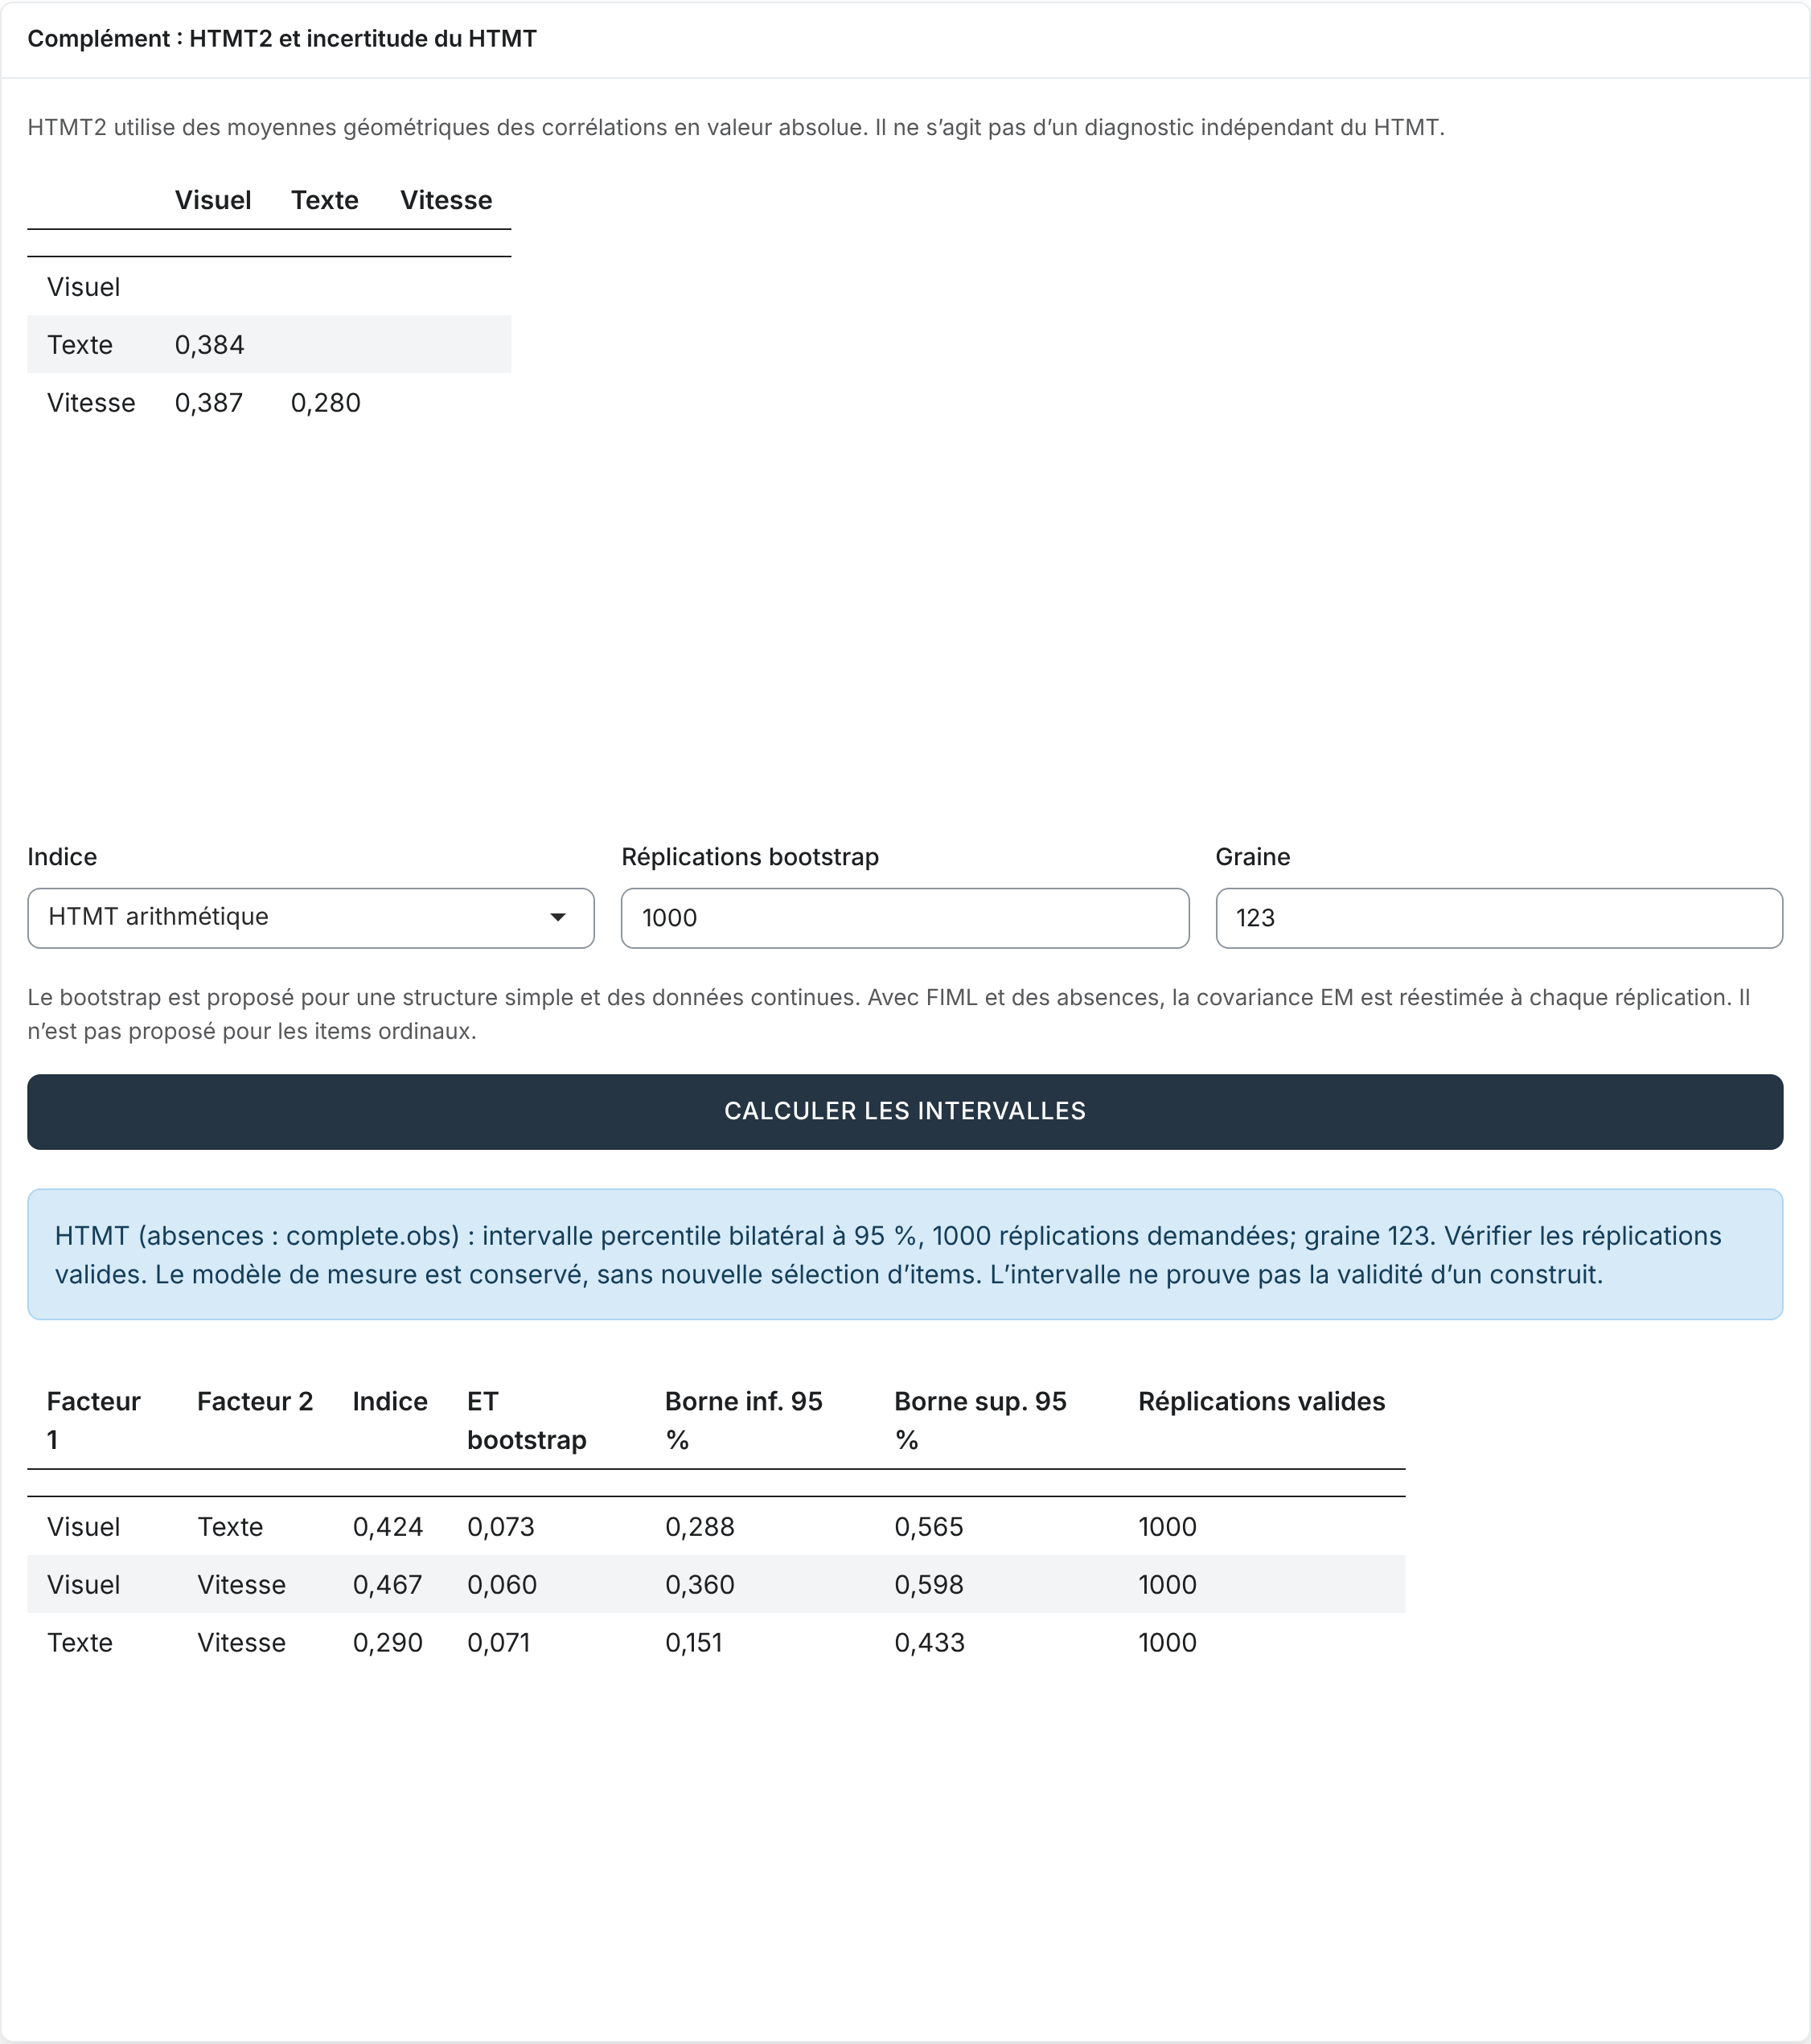
\includegraphics[width=1\linewidth,height=\textheight,keepaspectratio]{images/app/ch07_bootstrap.png}

}

\caption{\label{fig-app-bootstrap}\textbf{4. Interpréter} en
\textbf{Options avancées} : HTMT2, puis le calcul des intervalles
bootstrap du HTMT.}

\end{figure}%

La borne supérieure la plus haute, 0,598, reste très loin de 0,85 : même
en tenant compte de l'incertitude d'échantillonnage, aucune paire de
facteurs HS n'approche du repère. Les intervalles sont pourtant larges
(environ ± 0,13), ce qui rappelle qu'avec 301 élèves une valeur
ponctuelle reste approximative.

La proposition est limitée à une structure simple et à des indicateurs
continus. Avec FIML et des absences, la covariance utilisée pour le HTMT
est réestimée à chaque réplication. Le bootstrap proposé n'est pas
disponible pour les items ordinaux : il faudrait notamment réestimer les
corrélations catégorielles à chaque réplication selon une procédure
adaptée.

Ne remplacez pas une analyse ordinale par une analyse continue
uniquement pour débloquer ce bouton. Le choix de méthode doit rester
fondé sur la nature des variables et la question.

\section{Ce que l'on peut conclure}\label{ce-que-lon-peut-conclure}

Un résultat favorable peut soutenir l'idée que les ensembles
d'indicateurs ne paraissent pas entièrement confondus dans cette
analyse. Il ne prouve pas la validité globale de chaque construit. La
validité concerne l'argumentation qui relie les réponses, le sens
attribué aux scores et leur usage.

Une formulation prudente est : « Les corrélations factorielles et les
estimations du HTMT ne suggèrent pas ici une confusion complète des
dimensions. Cette observation est cohérente avec leur distinction, sous
les limites du modèle et de l'échantillon. » Ajoutez les difficultés
particulières lorsqu'elles existent.

Le cas de la démocratie politique montre l'autre extrême : la
corrélation entre \texttt{Democratie60} et \texttt{Democratie65} atteint
0,978. Les mêmes indicateurs observés à cinq ans d'écart ne se
distinguent presque pas; parler de deux construits différents serait
excessif. L'atelier B y revient.

\section{Laboratoire : deux lectures de la même
paire}\label{laboratoire-deux-lectures-de-la-muxeame-paire}

Sur HS, relevez les trois corrélations factorielles et les trois HTMT.
Repérez la paire la plus liée selon chaque lecture. Est-ce la même ?
Puis expliquez pourquoi une paire associée à un HTMT inférieur à 0,85 ne
peut pas être déclarée « valide » sur cette seule base. Si vous calculez
les intervalles, ajoutez une phrase sur leur largeur et les réplications
valides.

\begin{tcolorbox}[enhanced jigsaw, arc=.35mm, bottomrule=.15mm, bottomtitle=1mm, breakable, colback=white, colbacktitle=quarto-callout-tip-color!10!white, colframe=quarto-callout-tip-color-frame, coltitle=black, left=2mm, leftrule=.75mm, opacityback=0, opacitybacktitle=0.6, rightrule=.15mm, title={Réponse}, titlerule=0mm, toprule=.15mm, toptitle=1mm]

La paire la plus liée est Visuel -- Vitesse selon la corrélation
factorielle (0,471) et Visuel -- Vitesse selon le HTMT (0,467). Les deux
lectures concordent. Un HTMT sous 0,85 indique seulement que les deux
ensembles d'indicateurs ne se confondent pas empiriquement; la validité
d'un construit demande aussi un argument sur le contenu, les usages et
d'autres sources de preuve. Les intervalles bootstrap ont 1000
réplications valides sur 1 000 et une largeur d'environ 0,27.

\end{tcolorbox}

\begin{tcolorbox}[enhanced jigsaw, arc=.35mm, bottomrule=.15mm, bottomtitle=1mm, breakable, colback=white, colbacktitle=quarto-callout-important-color!10!white, colframe=quarto-callout-important-color-frame, coltitle=black, left=2mm, leftrule=.75mm, opacityback=0, opacitybacktitle=0.6, rightrule=.15mm, title={À retenir}, titlerule=0mm, toprule=.15mm, toptitle=1mm]

\begin{itemize}
\tightlist
\item
  Fornell--Larcker compare la racine de l'AVE aux corrélations entre
  facteurs, en valeur absolue.
\item
  Le HTMT se calcule sur les corrélations observées, indépendamment du
  modèle; le HTMT2 corrige l'effet de saturations inégales.
\item
  Les repères 0,85 et 0,90 se lisent avec l'incertitude : regardez la
  borne supérieure de l'intervalle.
\item
  Un critère favorable soutient une distinction empirique, pas la
  validité d'un construit.
\end{itemize}

\end{tcolorbox}

\section{Quiz}\label{quiz-6}

\begin{enumerate}
\def\labelenumi{\arabic{enumi}.}
\tightlist
\item
  Pourquoi le HTMT n'est-il pas calculé sur la matrice reproduite par le
  modèle ?
\item
  Une corrélation entre facteurs de −0,82 et une racine d'AVE de 0,75
  satisfont-elles le critère de Fornell et Larcker ?
\item
  Pourquoi le bootstrap du HTMT n'est-il pas offert avec des indicateurs
  ordinaux ?
\item
  Deux facteurs ont une corrélation de 0,98. Que conclure ?
\end{enumerate}

\begin{tcolorbox}[enhanced jigsaw, arc=.35mm, bottomrule=.15mm, bottomtitle=1mm, breakable, colback=white, colbacktitle=quarto-callout-tip-color!10!white, colframe=quarto-callout-tip-color-frame, coltitle=black, left=2mm, leftrule=.75mm, opacityback=0, opacitybacktitle=0.6, rightrule=.15mm, title={Réponses}, titlerule=0mm, toprule=.15mm, toptitle=1mm]

\begin{enumerate}
\def\labelenumi{\arabic{enumi}.}
\tightlist
\item
  Il redonnerait à peu près les corrélations factorielles et ne
  contrôlerait plus rien.
\item
  Non : 0,82 dépasse 0,75 en valeur absolue.
\item
  Chaque réplication exigerait de réestimer les corrélations
  polychoriques, une procédure plus lourde que l'application ne propose
  pas.
\item
  Que les deux ensembles d'indicateurs se distinguent à peine; il faut
  discuter le contenu partagé avant de parler de deux construits.
\end{enumerate}

\end{tcolorbox}

\bookmarksetup{startatroot}

\chapter{Analyser des réponses binaires et ordinales}\label{sec-ordinal}

\begin{tcolorbox}[enhanced jigsaw, arc=.35mm, bottomrule=.15mm, bottomtitle=1mm, breakable, colback=white, colbacktitle=quarto-callout-note-color!10!white, colframe=quarto-callout-note-color-frame, coltitle=black, left=2mm, leftrule=.75mm, opacityback=0, opacitybacktitle=0.6, rightrule=.15mm, title={Objectifs du chapitre}, titlerule=0mm, toprule=.15mm, toptitle=1mm]

\begin{itemize}
\tightlist
\item
  Comprendre la représentation d'une réponse catégorielle par une
  réponse latente et des seuils.
\item
  Déclarer des items ordinaux et choisir WLSMV.
\item
  Lire les versions standard, \emph{scaled} et \emph{robust} d'un même
  indice.
\item
  Situer la cible de la fiabilité dans une analyse ordinale.
\end{itemize}

\end{tcolorbox}

\begin{tcolorbox}[enhanced jigsaw, arc=.35mm, bottomrule=.15mm, bottomtitle=1mm, breakable, colback=white, colbacktitle=quarto-callout-tip-color!10!white, colframe=quarto-callout-tip-color-frame, coltitle=black, left=2mm, leftrule=.75mm, opacityback=0, opacitybacktitle=0.6, rightrule=.15mm, title={Idée centrale}, titlerule=0mm, toprule=.15mm, toptitle=1mm]

Un code 0, 1, 2 ou 3 n'est pas une mesure à intervalles égaux. L'AFC
ordinale suppose une réponse continue cachée sous chaque item et estime
les \textbf{seuils} qui la découpent en catégories. Les corrélations
analysées sont alors polychoriques, et les indices portent sur ces
réponses latentes.

\end{tcolorbox}

\section{Le nombre écrit dans la cellule ne définit pas la
mesure}\label{le-nombre-uxe9crit-dans-la-cellule-ne-duxe9finit-pas-la-mesure}

Une réponse correcte codée 1 et incorrecte codée 0 est une catégorie
binaire. Une réponse d'intensité allant de 0 à 3 est ordonnée, mais les
distances entre catégories ne sont pas automatiquement des unités égales
de la propriété mesurée. Ces nombres ne doivent pas être traités comme
continus simplement parce qu'ils sont stockés dans des colonnes
numériques.

Dans une AFC ordinale, on représente chaque réponse catégorielle à
partir d'une réponse latente continue et de \textbf{seuils}. La
catégorie observée dépend de l'intervalle dans lequel se situe cette
réponse sous-jacente. Ce modèle permet de distinguer la distribution des
catégories et les hypothèses sur les réponses latentes.

\begin{figure}[htbp]

\centering{

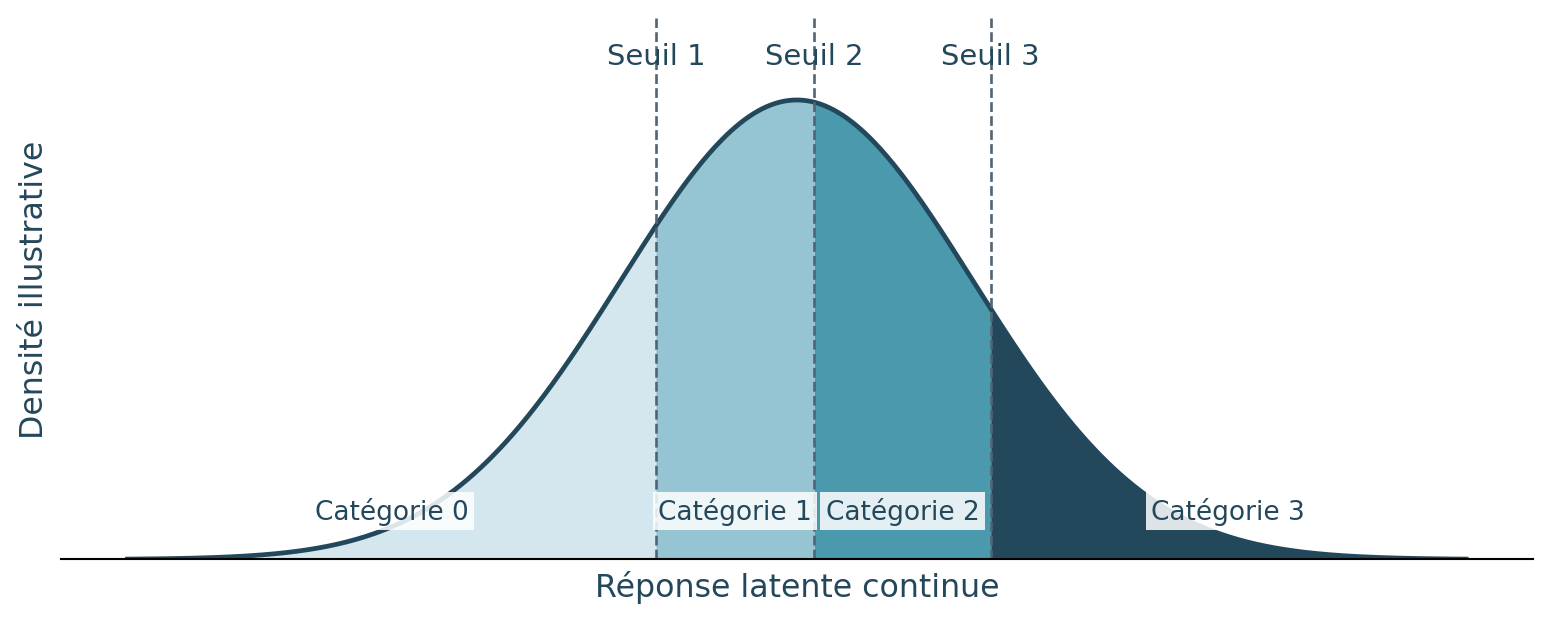
\includegraphics[width=0.9\linewidth,height=\textheight,keepaspectratio]{images/seuils.png}

}

\caption{\label{fig-seuils}Les seuils découpent une réponse latente
continue en catégories observées. Illustration conceptuelle, sans
paramètres estimés.}

\end{figure}%

Un item binaire possède un seuil; un item à quatre catégories ordonnées
possède trois seuils, si toutes ces catégories sont effectivement
observées et identifiables dans l'analyse. Des catégories très rares ou
absentes peuvent poser des difficultés.

\section{Déclarer les items et choisir
l'estimateur}\label{duxe9clarer-les-items-et-choisir-lestimateur}

Dans \textbf{Modèle \& Spécification}, les contrôles \textbf{Items
ordinaux} permettent de cocher les indicateurs concernés. Vérifiez ces
déclarations pour chaque facteur. \textbf{Tout sélectionner} s'applique
au groupe d'indicateurs du facteur affiché.

\begin{figure}[htbp]

\centering{

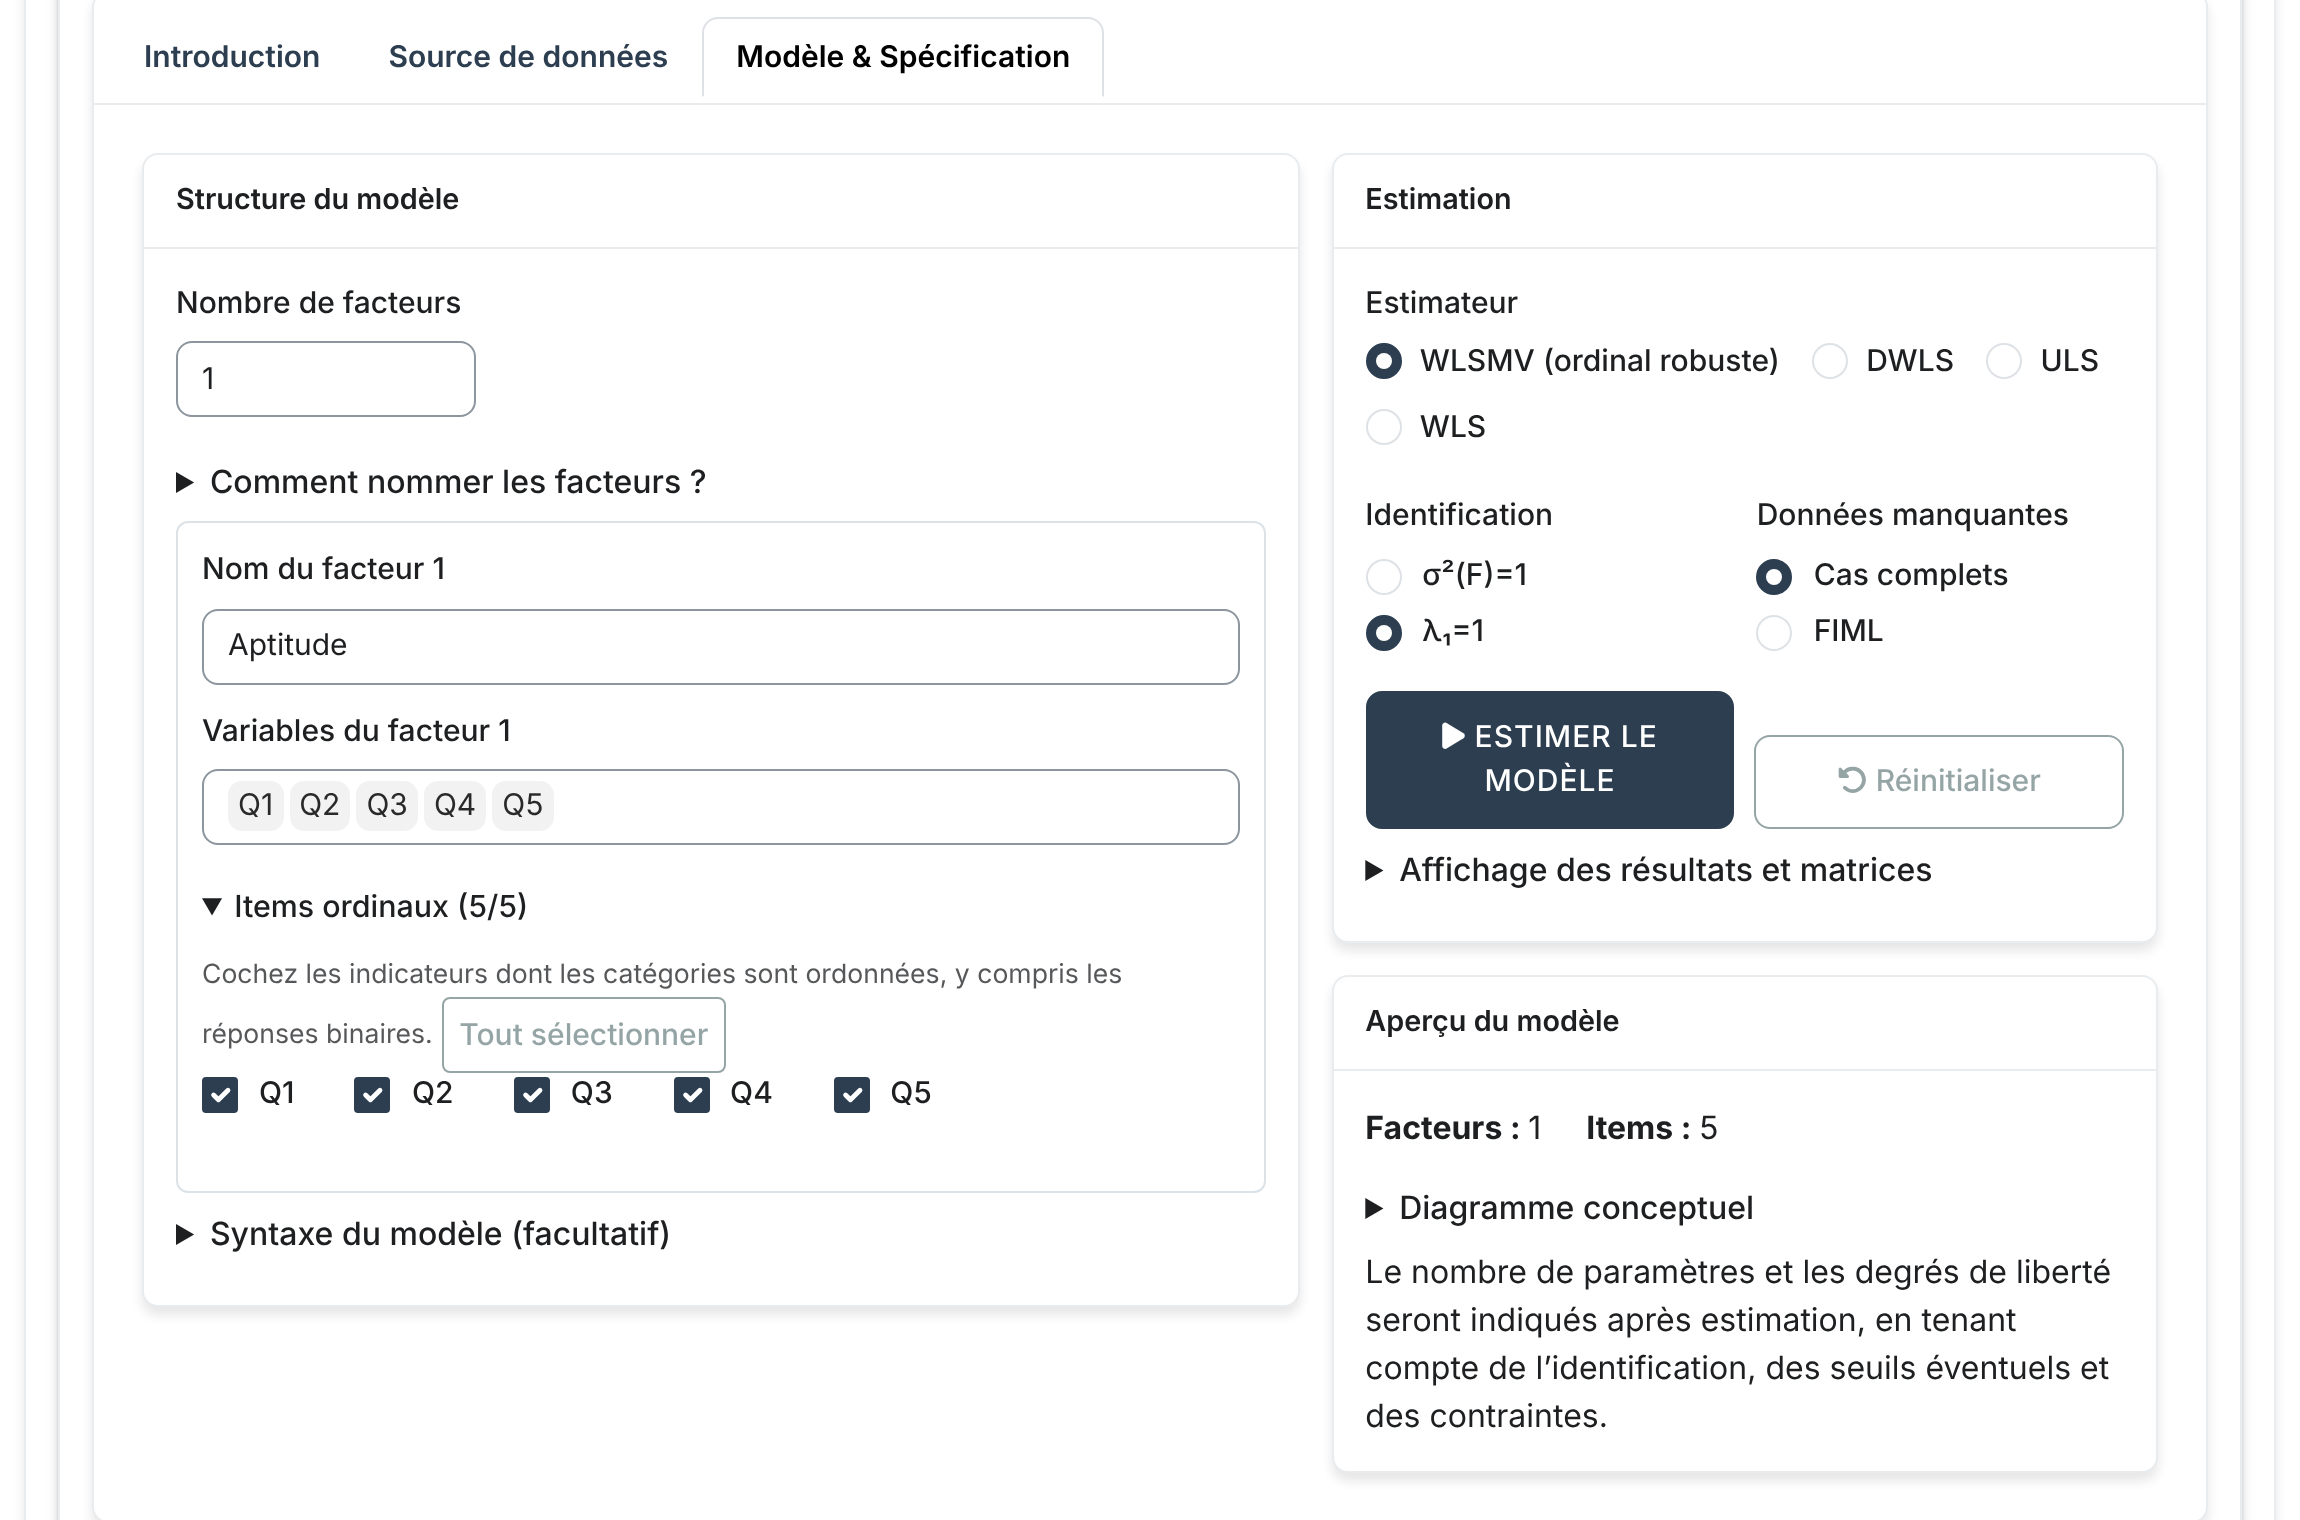
\includegraphics[width=1\linewidth,height=\textheight,keepaspectratio]{images/app/ch08_modele_lsat6.png}

}

\caption{\label{fig-app-lsat6}\textbf{Modèle \& Spécification} après le
chargement du LSAT 6 : un facteur \texttt{Aptitude}, cinq items déclarés
ordinaux (5/5) et l'estimateur WLSMV, seul choisi parmi les estimateurs
adaptés.}

\end{figure}%

Les modèles réels binaires ou ordinaux fournis sont déjà préparés avec
\textbf{WLSMV} après \textbf{Charger cet exemple et son modèle}. Dans ce
contexte, l'estimation exploite des relations adaptées aux catégories,
avec des erreurs-types et un test corrigés. Le libellé technique de DWLS
peut aussi apparaître dans certaines sorties, car WLSMV s'appuie sur une
estimation pondérée diagonale et des corrections supplémentaires
(\citeproc{ref-lavaancat}{Projet lavaan 2026b}).

Les choix \textbf{DWLS}, \textbf{ULS} ou \textbf{WLS} sont proposés pour
des usages plus spécifiques; ils ne sont pas des méthodes à départager
uniquement en choisissant celle qui donne l'indice le plus favorable. Ce
manuel retient WLSMV pour les activités ordinales. Lorsque des items
sont déclarés ordinaux, l'application refuse d'ailleurs ML et ML
robuste.

La combinaison FIML avec les indicateurs déclarés ordinaux n'est pas
disponible ici. Conservez \textbf{Cas complets} dans les exercices
concernés. Une analyse interrompue pour incompatibilité de réglages ne
doit pas être contournée en décochant artificiellement les items
ordinaux.

\section{Première activité avec LSAT
6}\label{premiuxe8re-activituxe9-avec-lsat-6}

Le LSAT 6 comporte cinq réponses binaires pour 1\,000 observations. Le
modèle de départ comporte un seul facteur \texttt{Aptitude}. Les
réponses sont développées à partir des effectifs des profils publiés;
leur ordre ne fournit pas des identifiants individuels d'origine
(\citeproc{ref-bock1970}{Bock et Lieberman 1970}).

\begin{enumerate}
\def\labelenumi{\arabic{enumi}.}
\tightlist
\item
  Dans \textbf{Données réelles}, sélectionnez \textbf{LSAT 6}.
\item
  Cliquez sur \textbf{Charger cet exemple et son modèle}.
\item
  Vérifiez un seul facteur et les indicateurs \texttt{Q1}, \texttt{Q2},
  \texttt{Q3}, \texttt{Q4}, \texttt{Q5}.
\item
  Vérifiez \textbf{Items ordinaux (5/5)}, \textbf{WLSMV} et \textbf{Cas
  complets}.
\item
  Estimez, puis ouvrez \textbf{Statistiques Descriptives → Normalité
  univariée}.
\item
  Vérifiez qu'une note remplace les tests continus; il ne manque pas un
  tableau utile.
\item
  Consultez les paramètres, les seuils et \textbf{4. Interpréter}.
\end{enumerate}

\begin{figure}[htbp]

\centering{

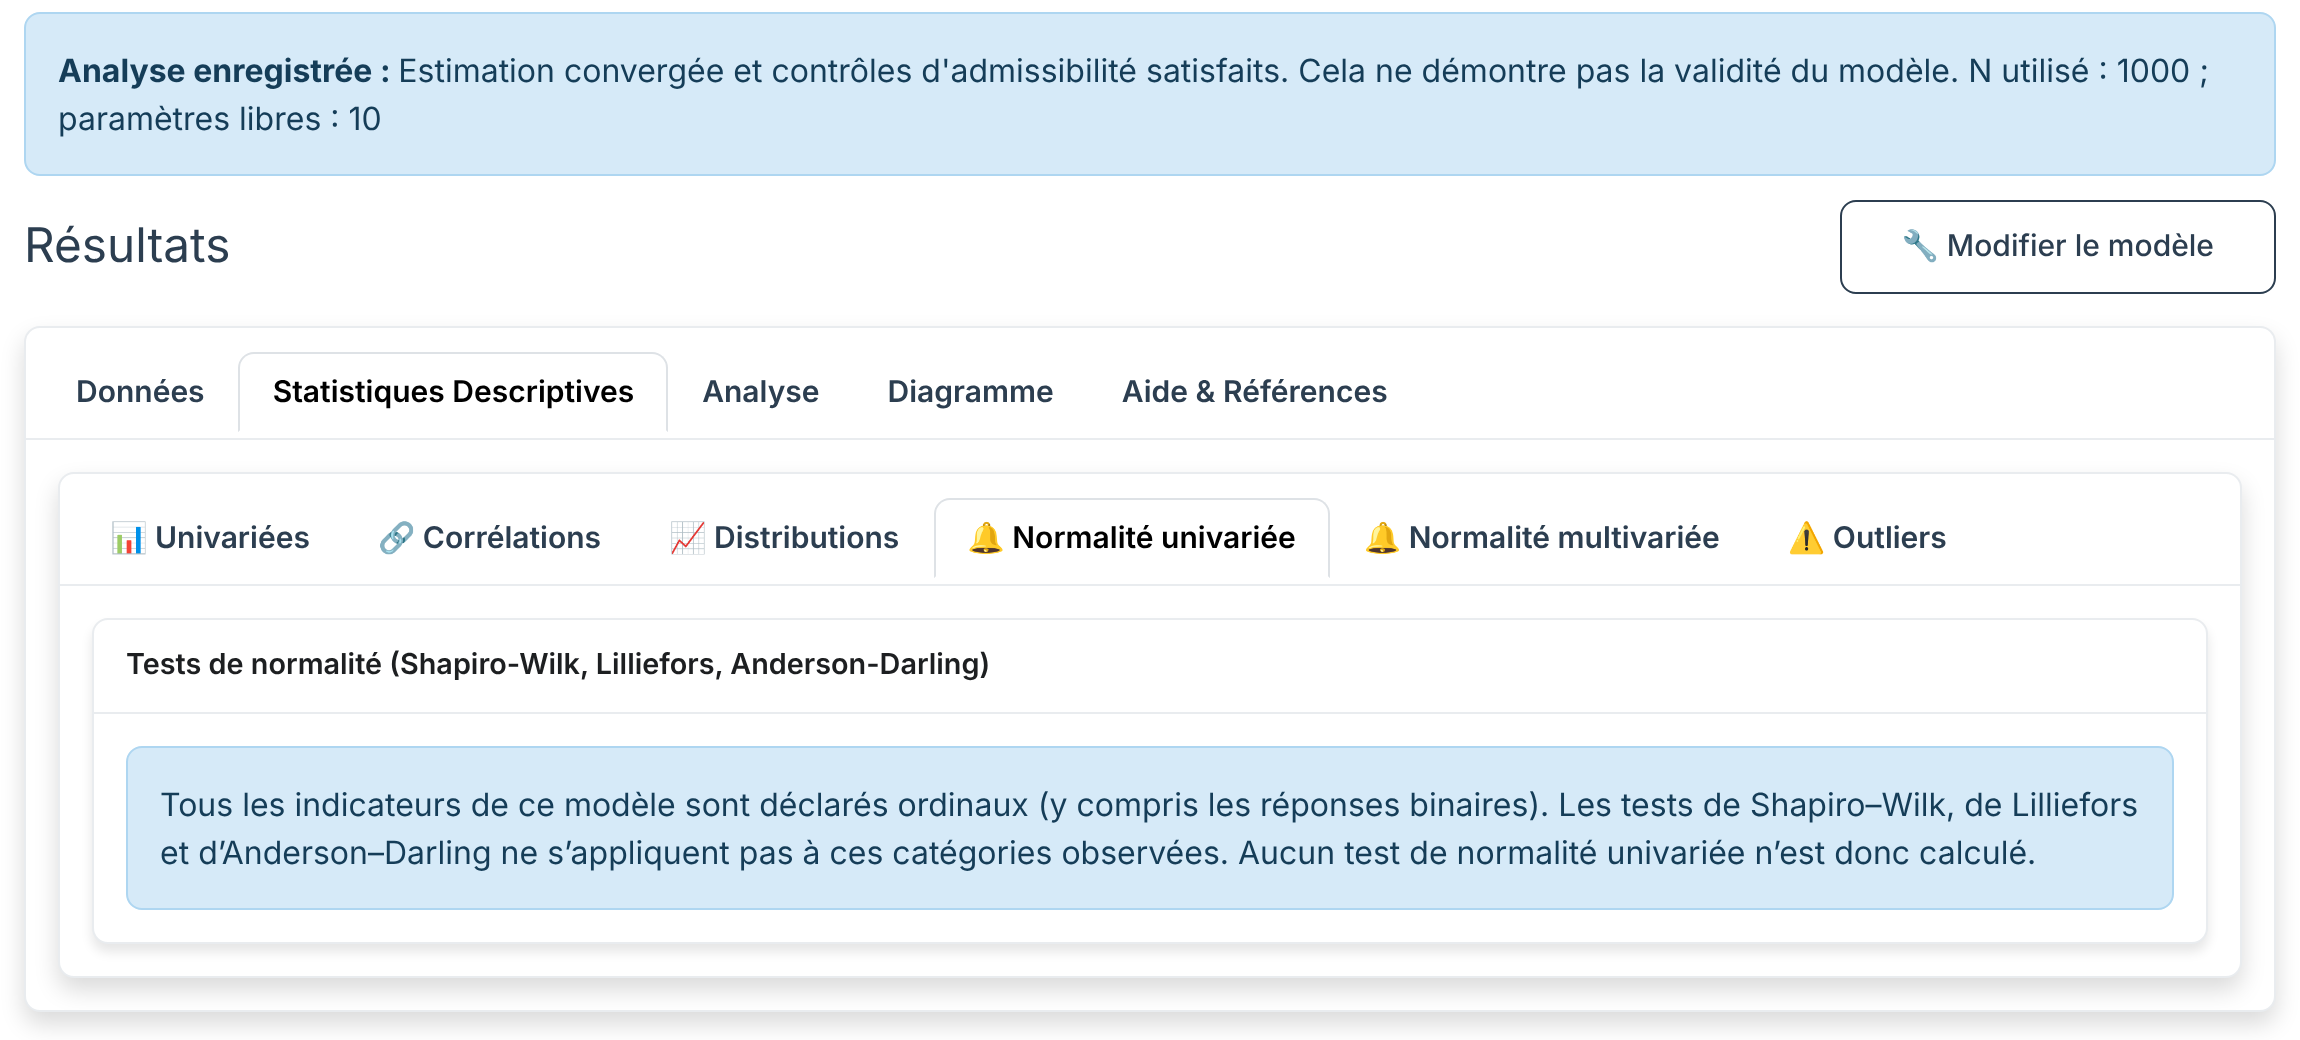
\includegraphics[width=1\linewidth,height=\textheight,keepaspectratio]{images/app/ch08_normalite_note.png}

}

\caption{\label{fig-app-note}\textbf{Normalité univariée} avec des items
déclarés ordinaux : une note remplace le tableau des tests.}

\end{figure}%

\begin{figure}[htbp]

\centering{

\includegraphics[width=0.88\linewidth,height=\textheight,keepaspectratio]{08-ordinal_files/figure-pdf/fig-lsat6-seuils-1.png}

}

\caption{\label{fig-lsat6-seuils}Seuils estimés des cinq items du LSAT 6
sur l'échelle de la réponse latente (moyenne 0, écart type 1). Plus le
seuil est bas, plus l'item est facile : la proportion attendue de
réponses correctes est l'aire de la courbe normale au-delà du seuil.}

\end{figure}%

Les cinq seuils sont négatifs : tous les items sont réussis par une
majorité de candidats. Q1 est le plus facile (seuil −1,43), Q3 le plus
difficile (seuil −0,13).

Le modèle a 5 degrés de liberté. Un RMSEA nul ou un CFI de 1 dans cet
exemple ne signifie pas que l'instrument est parfait. Ces résultats
doivent être replacés dans le modèle, l'effectif, les degrés de liberté
et l'incertitude des tests.

Reprenez ensuite \textbf{LSAT 7} avec son modèle préparé. Analysez les
deux fichiers séparément : les lignes de LSAT 6 et LSAT 7 ne doivent pas
être appariées comme si elles provenaient des mêmes personnes.

\section{Le cas MSQ}\label{le-cas-msq}

Le fichier proposé dans l'application conserve vingt adjectifs d'affect
et la première occasion de mesure pour 3\,032 participants. Les réponses
vont de \textbf{0 = pas du tout} à \textbf{3 = beaucoup}, à propos du
moment présent. Le modèle oppose deux ensembles corrélés :
\texttt{AffectPositif} et \texttt{AffectNegatif}.

Cette sélection est un sous-ensemble documenté du MSQ. Elle ne
correspond pas à une nouvelle collecte indépendante de l'instrument
PANAS, même si les clés d'affect renvoient à cette littérature. Les
données réunissent plusieurs études et conditions; la simplicité du
modèle reste une hypothèse (\citeproc{ref-watson1988}{Watson et al.
1988}).

Chargez \textbf{MSQ}, puis \textbf{Charger cet exemple et son modèle}.
Vérifiez dix indicateurs par facteur, vingt déclarations ordinales,
WLSMV et les cas complets. \textbf{2\,951 participants} disposent de
réponses complètes pour ces vingt indicateurs; 81 lignes ne sont pas
utilisées dans cette estimation par cas complets.

\section{Lire les versions des indices sur
MSQ}\label{lire-les-versions-des-indices-sur-msq}

Les valeurs suivantes proviennent du même modèle et des mêmes données.
Elles illustrent pourquoi il faut annoncer la version lue :

\Needspace{7\baselineskip}

{

\begin{longtable}[]{@{}lrr@{}}

\caption{\label{tbl-msq-versions}Trois versions du CFI et du RMSEA pour
le même modèle MSQ (WLSMV, 2\,951 cas complets).}

\tabularnewline

\toprule\noalign{}
Version & CFI & RMSEA \\
\midrule\noalign{}
\endhead
\bottomrule\noalign{}
\endlastfoot
Standard & 0,953 & 0,115 \\
Scaled & 0,908 & 0,103 \\
Robust & 0,760 & 0,152 \\

\end{longtable}

}

\begin{figure}[htbp]

\centering{

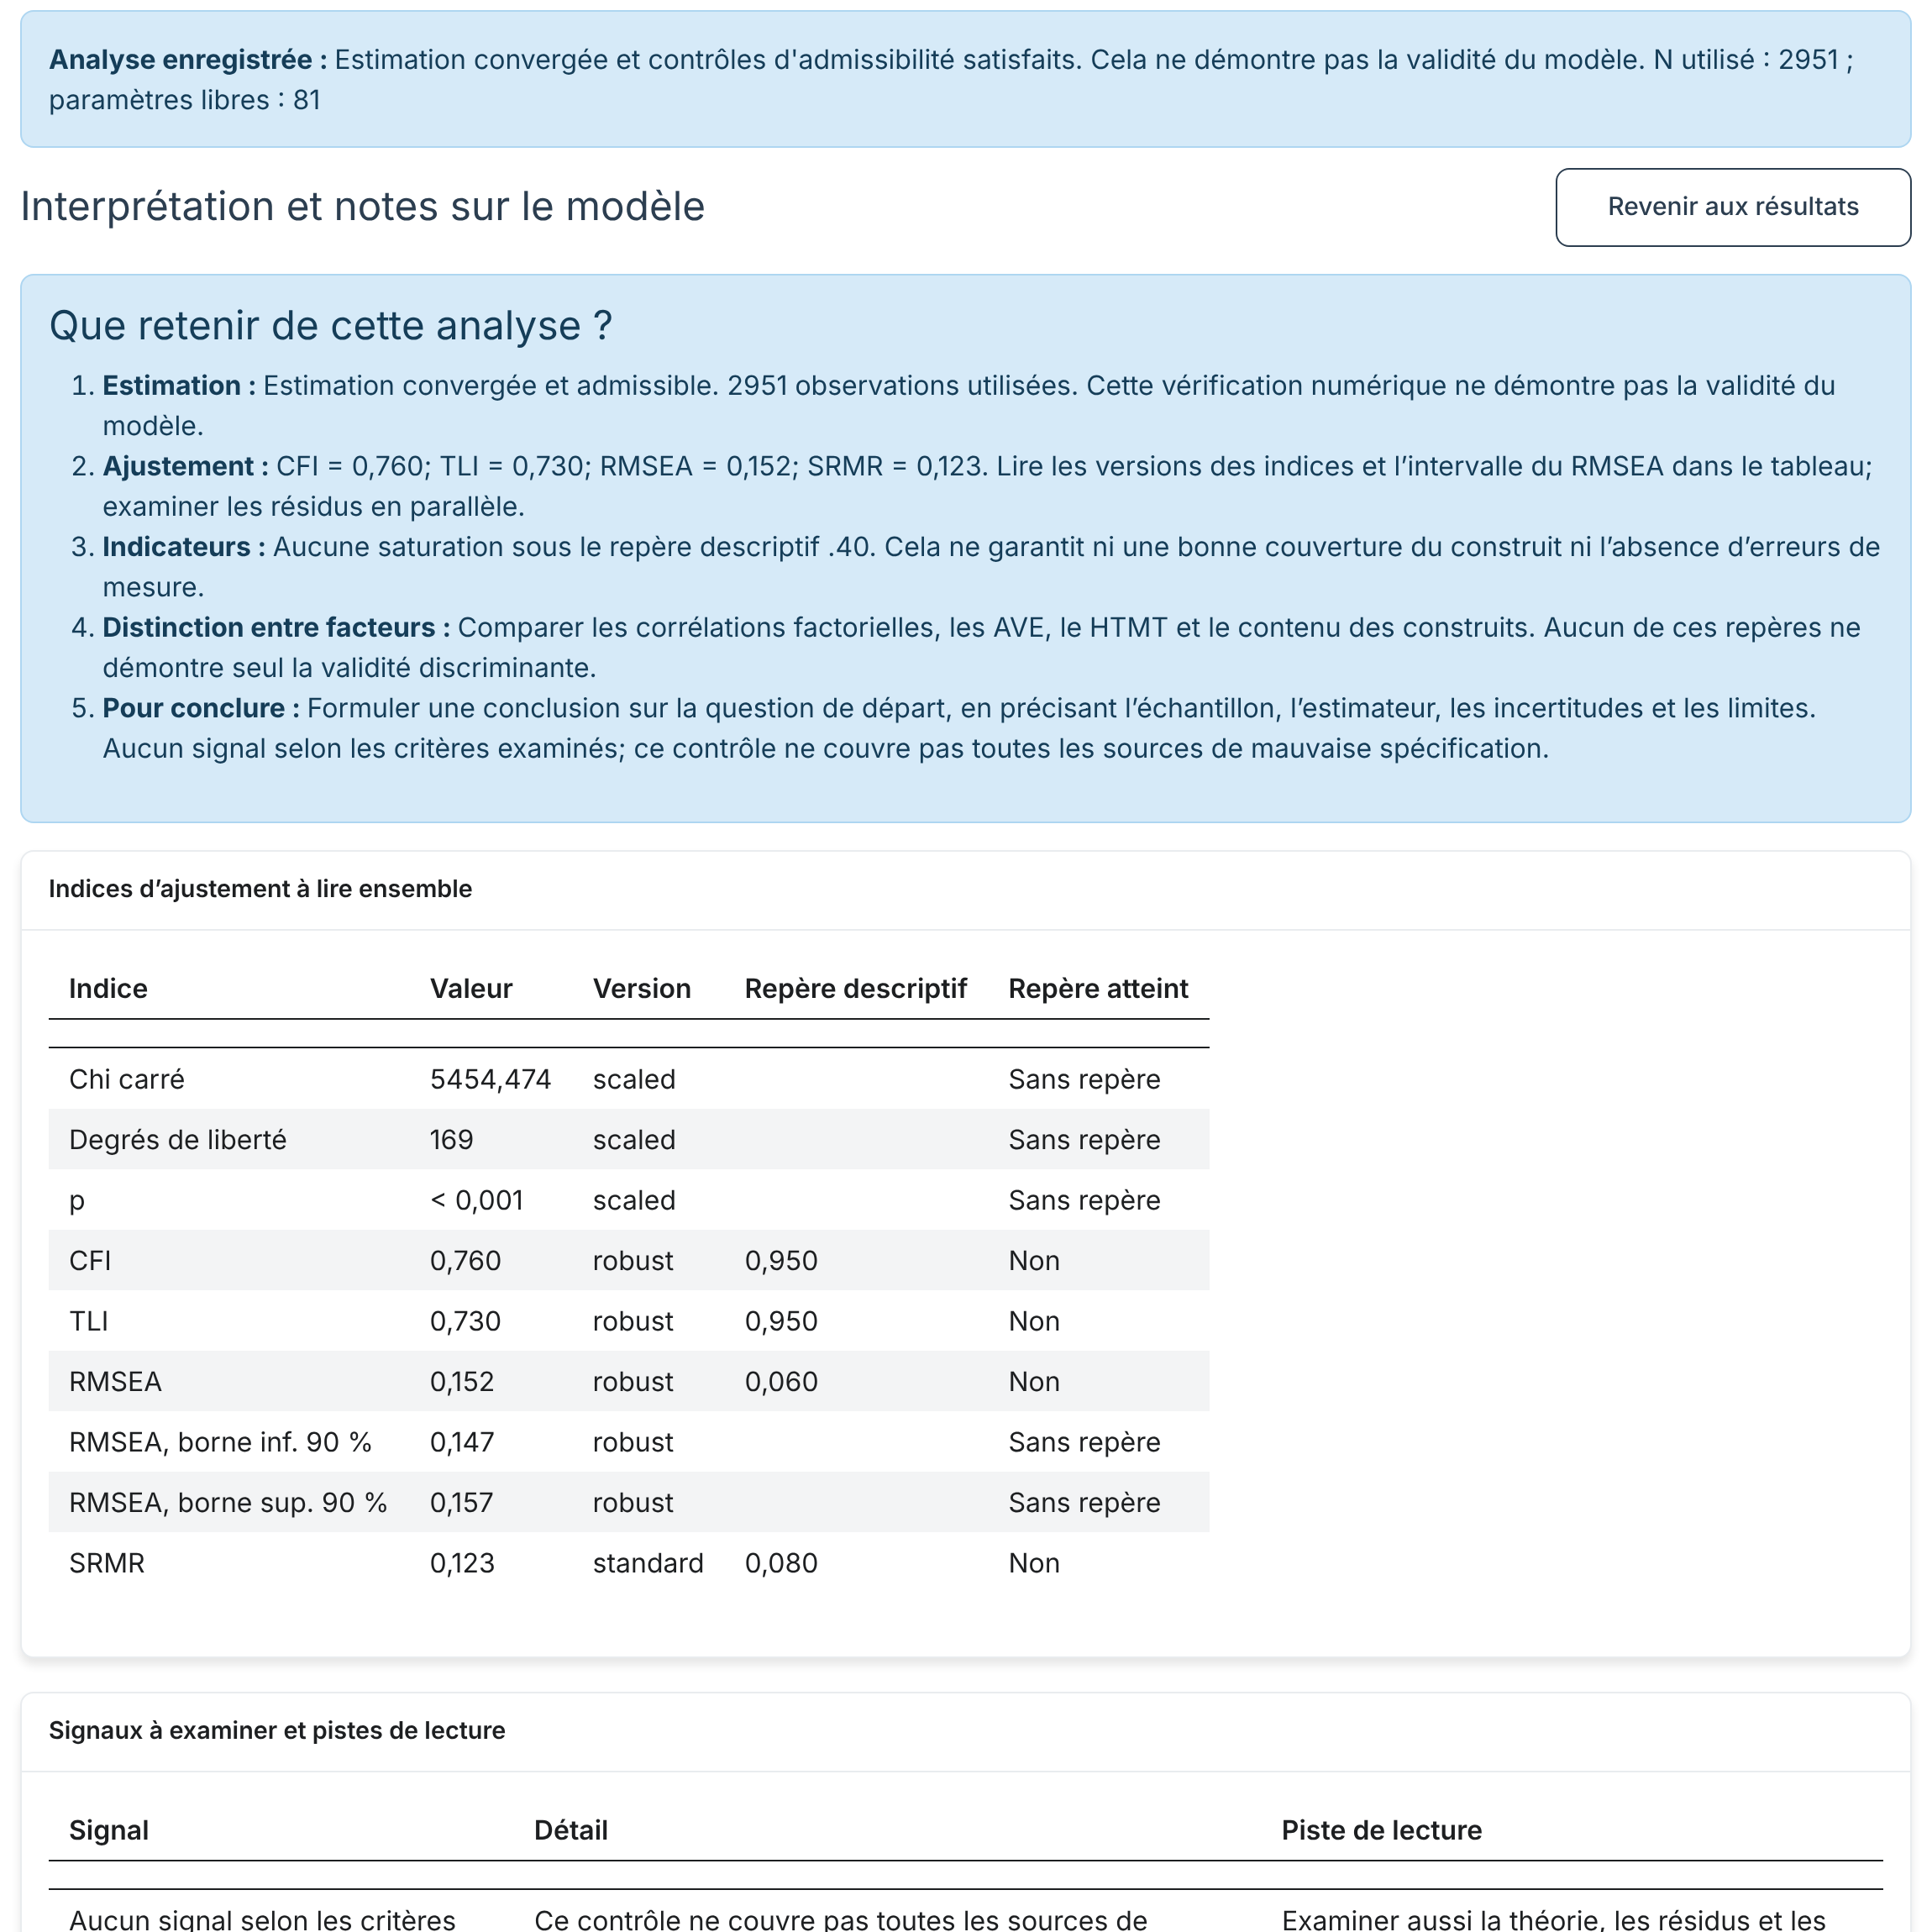
\includegraphics[width=1\linewidth,height=\textheight,keepaspectratio]{images/app/ch08_msq_interpreter.png}

}

\caption{\label{fig-app-msq}\textbf{4. Interpréter} sur MSQ : les
indices repris dans la synthèse sont les versions robustes (CFI, TLI,
RMSEA) et \emph{scaled} (chi carré), comme l'indique la colonne de
version.}

\end{figure}%

Dans \textbf{4. Interpréter}, l'application privilégie les versions
robustes disponibles pour CFI et RMSEA et indique leur version. Un CFI
standard de 0,953 ne contredit donc pas un CFI robuste de 0,760 dans la
synthèse. Vous ne comparez pas la même correction de l'indice.

Le SRMR vaut 0,123. La synthèse des diagnostics ne soutient pas une
reproduction satisfaisante de toutes les relations par ce modèle simple.
Le nombre important de répondants et des saturations souvent fortes ne
font pas disparaître ces écarts.

\section{Fiabilité et cible de
l'indice}\label{fiabilituxe9-et-cible-de-lindice}

Dans les suppléments, les omégas des deux dimensions du MSQ sont élevés
(0,940 et 0,934). Ils portent ici sur les réponses latentes continues.
Ils ne suffisent pas à valider l'ajustement global et ne décrivent pas
directement la fiabilité d'une somme des catégories observées.

Pour le facteur négatif notamment, plusieurs adjectifs très proches
peuvent partager du contenu spécifique. Avant de retirer des items ou
d'ajouter des covariances résiduelles, formulez ce que vous chercheriez
à représenter et quel effet cela aurait sur la définition du construit.

\section{Laboratoire : deux sections du
LSAT}\label{laboratoire-deux-sections-du-lsat}

Estimez LSAT 6 puis LSAT 7 avec leurs modèles préparés. Pour chacun,
relevez l'effectif, les degrés de liberté, le CFI et le RMSEA
\textbf{dans leurs trois versions} (sortie détaillée de \textbf{Analyse
→ Analyse de base → Résultats}). Quelle section le modèle à un facteur
décrit-il le mieux ? Pourquoi faut-il préciser la version avant de
répondre ?

\begin{tcolorbox}[enhanced jigsaw, arc=.35mm, bottomrule=.15mm, bottomtitle=1mm, breakable, colback=white, colbacktitle=quarto-callout-tip-color!10!white, colframe=quarto-callout-tip-color-frame, coltitle=black, left=2mm, leftrule=.75mm, opacityback=0, opacitybacktitle=0.6, rightrule=.15mm, title={Réponse}, titlerule=0mm, toprule=.15mm, toptitle=1mm]

\Needspace{10\baselineskip}

{\def\LTcaptype{none} % do not increment counter
\begin{longtable}[]{@{}llrr@{}}
\toprule\noalign{}
Section & Version & CFI & RMSEA \\
\midrule\noalign{}
\endhead
\bottomrule\noalign{}
\endlastfoot
LSAT 6 & Standard & 1,000 & 0,000 \\
LSAT 6 & Scaled & 1,000 & 0,000 \\
LSAT 6 & Robust & 1,000 & 0,000 \\
LSAT 7 & Standard & 0,982 & 0,029 \\
LSAT 7 & Scaled & 0,969 & 0,037 \\
LSAT 7 & Robust & 0,943 & 0,079 \\
\end{longtable}
}

Les deux analyses utilisent 1\,000 observations et 5 degrés de liberté.
Le modèle décrit très bien le LSAT 6 dans toutes les versions. Pour le
LSAT 7, le RMSEA passe de 0,029 (standard) à 0,079 (robuste) : selon la
version citée, on conclurait à un ajustement excellent ou seulement
acceptable. Il faut donc toujours nommer la version. Les deux
échantillons étant distincts, aucun test de différence entre eux n'est
approprié.

\end{tcolorbox}

\begin{tcolorbox}[enhanced jigsaw, arc=.35mm, bottomrule=.15mm, bottomtitle=1mm, breakable, colback=white, colbacktitle=quarto-callout-important-color!10!white, colframe=quarto-callout-important-color-frame, coltitle=black, left=2mm, leftrule=.75mm, opacityback=0, opacitybacktitle=0.6, rightrule=.15mm, title={À retenir}, titlerule=0mm, toprule=.15mm, toptitle=1mm]

\begin{itemize}
\tightlist
\item
  Des codes ordinaux ne sont pas des mesures à intervalles égaux :
  déclarez les items ordinaux et utilisez WLSMV.
\item
  Les seuils situent les catégories sur l'échelle de la réponse latente.
\item
  Une même analyse produit plusieurs versions d'un indice : nommez celle
  que vous citez.
\item
  Oméga ordinal décrit la réponse latente, pas la somme des catégories
  observées.
\end{itemize}

\end{tcolorbox}

\section{Quiz}\label{quiz-7}

\begin{enumerate}
\def\labelenumi{\arabic{enumi}.}
\tightlist
\item
  Un item à cinq catégories toutes observées possède combien de seuils ?
\item
  Pourquoi l'application refuse-t-elle ML lorsque des items sont
  déclarés ordinaux ?
\item
  Le CFI standard du MSQ vaut 0,953. Peut-on écrire que le modèle
  s'ajuste bien ?
\item
  Pourquoi ne peut-on pas utiliser FIML avec ces items ordinaux dans
  l'application ?
\end{enumerate}

\begin{tcolorbox}[enhanced jigsaw, arc=.35mm, bottomrule=.15mm, bottomtitle=1mm, breakable, colback=white, colbacktitle=quarto-callout-tip-color!10!white, colframe=quarto-callout-tip-color-frame, coltitle=black, left=2mm, leftrule=.75mm, opacityback=0, opacitybacktitle=0.6, rightrule=.15mm, title={Réponses}, titlerule=0mm, toprule=.15mm, toptitle=1mm]

\begin{enumerate}
\def\labelenumi{\arabic{enumi}.}
\tightlist
\item
  Quatre.
\item
  ML suppose des indicateurs continus; il traiterait les codes comme des
  mesures à intervalles égaux.
\item
  Non. Les versions corrigées (CFI robuste 0,760) et le SRMR (0,123)
  indiquent des écarts importants; citer seulement la version favorable
  serait trompeur.
\item
  FIML est proposé ici avec ML ou ML robuste, donc pour des indicateurs
  continus; l'estimation ordinale passe par les corrélations
  polychoriques et les cas complets.
\end{enumerate}

\end{tcolorbox}

\bookmarksetup{startatroot}

\chapter{Comprendre et traiter les données
manquantes}\label{sec-absences}

\begin{tcolorbox}[enhanced jigsaw, arc=.35mm, bottomrule=.15mm, bottomtitle=1mm, breakable, colback=white, colbacktitle=quarto-callout-note-color!10!white, colframe=quarto-callout-note-color-frame, coltitle=black, left=2mm, leftrule=.75mm, opacityback=0, opacitybacktitle=0.6, rightrule=.15mm, title={Objectifs du chapitre}, titlerule=0mm, toprule=.15mm, toptitle=1mm]

\begin{itemize}
\tightlist
\item
  Distinguer les lignes chargées, les observations utilisées et les cas
  d'un diagnostic.
\item
  Comparer l'analyse des cas complets et FIML sur un même fichier.
\item
  Situer les hypothèses MCAR, MAR et MNAR sans prétendre les vérifier
  par un test.
\item
  Rédiger une note de méthode qui annonce les absences et leur
  traitement.
\end{itemize}

\end{tcolorbox}

\begin{tcolorbox}[enhanced jigsaw, arc=.35mm, bottomrule=.15mm, bottomtitle=1mm, breakable, colback=white, colbacktitle=quarto-callout-tip-color!10!white, colframe=quarto-callout-tip-color-frame, coltitle=black, left=2mm, leftrule=.75mm, opacityback=0, opacitybacktitle=0.6, rightrule=.15mm, title={Idée centrale}, titlerule=0mm, toprule=.15mm, toptitle=1mm]

Le traitement des absences est une hypothèse, pas un correctif. Les cas
complets supposent que les personnes retenues représentent bien
l'ensemble; FIML suppose que l'absence s'explique par l'information
observée. Aucun indice d'ajustement ne dit laquelle de ces hypothèses
est vraie.

\end{tcolorbox}

\section{Trois effectifs à
distinguer}\label{trois-effectifs-uxe0-distinguer}

Le nombre de lignes chargées, le nombre d'observations utilisées pour
estimer le modèle et le nombre de cas disponibles pour un diagnostic
peuvent différer. L'application conserve ces informations à des endroits
différents parce qu'elles répondent à des opérations différentes.

Pour le MSQ, 3\,032 lignes sont chargées, mais 2\,951 sont complètes
pour les vingt indicateurs du modèle proposé. Pour SAPA, les 1\,525
lignes donnent 1\,248 cas complets sur les seize indicateurs. Une ligne
exclue de l'estimation ne disparaît pas du fichier original.

\section{Cas complets}\label{cas-complets}

\textbf{Cas complets} utilise les personnes qui possèdent des réponses à
tous les indicateurs analysés. La méthode est simple à décrire, mais
peut diminuer l'information disponible et modifier la composition de
l'échantillon. Ses propriétés dépendent notamment de la manière dont les
absences se produisent.

Le simple fait qu'il reste un grand nombre de personnes ne démontre pas
que les exclusions sont sans conséquence. Comparez les personnes
retenues et non retenues sur les informations disponibles lorsque cette
vérification est possible. Documentez les absences par variable et par
motif de réponse.

\section{FIML}\label{fiml}

\textbf{FIML} exploite les informations observées des personnes
partiellement renseignées dans une estimation par maximum de
vraisemblance. Il ne remplace pas chaque cellule vide par une valeur
unique. Dans l'application, il est proposé avec des indicateurs continus
et \textbf{ML} ou \textbf{ML robuste}.

L'approche repose sur des hypothèses concernant le modèle et le
mécanisme d'absence, notamment une ignorabilité de type MAR dans les
conditions appropriées. MAR signifie que, conditionnellement aux
informations observées pertinentes, l'absence ne dépend plus des valeurs
manquantes elles-mêmes. Ce mécanisme ne se démontre pas en obtenant une
valeur de p favorable à un test de normalité.

\Needspace{7\baselineskip}

{\def\LTcaptype{none} % do not increment counter
\begin{longtable}[]{@{}
  >{\raggedright\arraybackslash}p{(\linewidth - 6\tabcolsep) * \real{0.2500}}
  >{\raggedright\arraybackslash}p{(\linewidth - 6\tabcolsep) * \real{0.2500}}
  >{\raggedright\arraybackslash}p{(\linewidth - 6\tabcolsep) * \real{0.2500}}
  >{\raggedright\arraybackslash}p{(\linewidth - 6\tabcolsep) * \real{0.2500}}@{}}
\toprule\noalign{}
\begin{minipage}[b]{\linewidth}\raggedright
Mécanisme
\end{minipage} & \begin{minipage}[b]{\linewidth}\raggedright
L'absence dépend\ldots{}
\end{minipage} & \begin{minipage}[b]{\linewidth}\raggedright
Cas complets
\end{minipage} & \begin{minipage}[b]{\linewidth}\raggedright
FIML
\end{minipage} \\
\midrule\noalign{}
\endhead
\bottomrule\noalign{}
\endlastfoot
MCAR & de rien qui soit lié aux variables & sans biais, moins précis &
sans biais \\
MAR & de variables observées & biais possible & sans biais si ces
variables sont dans le modèle \\
MNAR & des valeurs manquantes elles-mêmes & biais possible & biais
possible \\
\end{longtable}
}

MCAR est une hypothèse plus restrictive d'absence complètement
aléatoire. MNAR désigne des mécanismes qui dépendent encore de valeurs
non observées après conditionnement pertinent. Les données observées
seules ne permettent pas de trancher sans hypothèses supplémentaires
entre tous ces mécanismes. Une stratégie raisonnable combine
connaissance du recueil, examen descriptif et analyses de sensibilité
(\citeproc{ref-enders2010}{Enders 2010}).

FIML requiert ici une structure des moyennes, que l'application active
automatiquement avec ce choix. Il ne devient pas une méthode ordinale en
présence de catégories simplement parce que celles-ci sont codées
numériquement (\citeproc{ref-lavaanest}{Projet lavaan 2026c}).

\section{Exercice avec un fichier dérivé
explicite}\label{exercice-avec-un-fichier-duxe9rivuxe9-explicite}

\textbf{But.} Constater la différence entre exclusion complète et
utilisation de réponses partielles. Le fichier
\texttt{HS\_absences\_pedagogiques.csv} est un dérivé des données HS,
fourni dans le dossier \texttt{donnees} du complément distribué avec ce
manuel. Il ne représente pas un nouveau recueil réel.

Trois séries de trente cellules ont été vidées : \texttt{x2} aux lignes
de données 1 à 30, \texttt{x5} aux lignes 31 à 60, puis \texttt{x8} aux
lignes 61 à 90. Toutes les autres valeurs et toutes les lignes sont
conservées (90 cellules vides sur 301 lignes). Cette suppression est
déterministe; elle ne garantit pas un mécanisme MCAR ou MAR dans une
interprétation substantielle.

Si le complément n'a pas été remis, vous pouvez reproduire le fichier
sans R. Téléchargez les données HS depuis l'application et ouvrez le CSV
dans un tableur en conservant les colonnes d'origine. Avec l'en-tête en
ligne 1, videz uniquement les cellules de \texttt{x2} aux lignes 2 à 31,
de \texttt{x5} aux lignes 32 à 61 et de \texttt{x8} aux lignes 62 à 91.
Dans le fichier complet à quinze colonnes, ces plages sont H2:H31,
K32:K61 et N62:N91. Vérifiez d'abord les en-têtes : une réorganisation
de colonnes modifierait les lettres. N'effacez aucune ligne entière.
Enregistrez une copie CSV sous le nom de l'exercice, avec des cellules
réellement vides.

\section{Première analyse par cas
complets}\label{premiuxe8re-analyse-par-cas-complets}

\begin{enumerate}
\def\labelenumi{\arabic{enumi}.}
\tightlist
\item
  Choisissez \textbf{Charger un fichier} et ouvrez le CSV dérivé.
\item
  Conservez les noms de colonnes en première ligne. Choisissez le
  séparateur qui reproduit quinze colonnes; la copie fournie utilise la
  virgule.
\item
  Dans le modèle, définissez \texttt{Visuel} avec \texttt{x1} à
  \texttt{x3}, \texttt{Texte} avec \texttt{x4} à \texttt{x6} et
  \texttt{Vitesse} avec \texttt{x7} à \texttt{x9}.
\item
  Ne déclarez aucun item ordinal. Choisissez \textbf{ML}, \textbf{λ₁=1}
  et \textbf{Cas complets}.
\item
  Estimez et relevez le nombre d'observations utilisées. Téléchargez un
  premier rapport.
\end{enumerate}

\begin{figure}[htbp]

\centering{

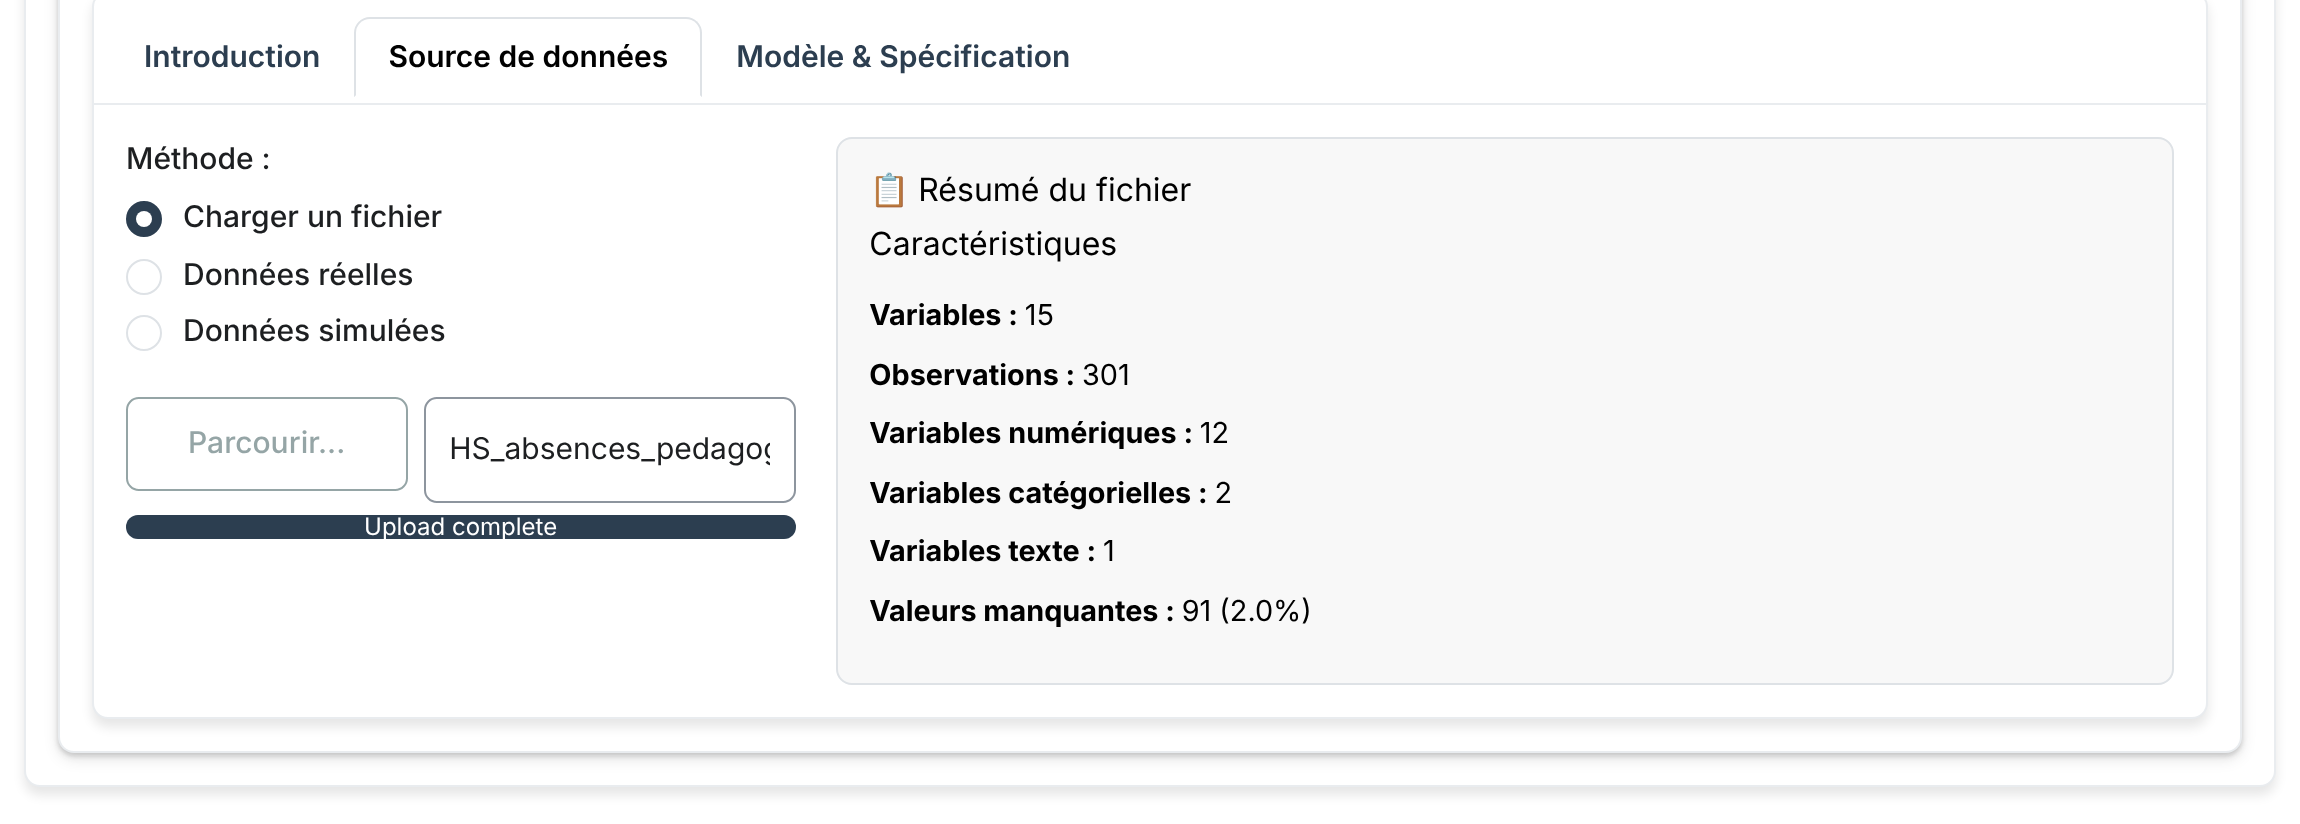
\includegraphics[width=1\linewidth,height=\textheight,keepaspectratio]{images/app/ch09_import.png}

}

\caption{\label{fig-app-import}\textbf{Charger un fichier} : le résumé
confirme 15 variables, 301 observations et 90 valeurs manquantes. Les
pourcentages portent sur l'ensemble des cellules du fichier.}

\end{figure}%

Vous devez retrouver \textbf{211 cas complets}. Si vous obtenez un autre
nombre, vérifiez les plages de cellules, les variables sélectionnées et
l'interprétation des cellules vides.

\section{Deuxième analyse avec
FIML}\label{deuxiuxe8me-analyse-avec-fiml}

Conservez exactement le fichier et les indicateurs, choisissez
\textbf{FIML}, puis estimez de nouveau. Les 301 personnes possèdent
encore au moins une réponse disponible; l'effectif utilisé est donc de
301. Téléchargez ce second rapport sous un autre nom.

\Needspace{7\baselineskip}

{

\begin{longtable}[]{@{}lrrrr@{}}

\caption{\label{tbl-absences}Le même modèle HS sur trois versions des
données : fichier original complet, fichier dérivé par cas complets et
fichier dérivé par FIML (ML).}

\tabularnewline

\toprule\noalign{}
Traitement & N & CFI & RMSEA & SRMR \\
\midrule\noalign{}
\endhead
\bottomrule\noalign{}
\endlastfoot
Original complet & 301 & 0,931 & 0,092 & 0,065 \\
Cas complets & 211 & 0,924 & 0,098 & 0,071 \\
FIML & 301 & 0,923 & 0,098 & 0,061 \\

\end{longtable}

}

Ce tableau fournit des repères, pas une compétition entre méthodes. Les
indices de la ligne Cas complets et de la ligne FIML ne portent pas sur
une information identique. Un SRMR plus faible ne suffit pas à démontrer
qu'une hypothèse sur les absences est vraie ou qu'un traitement est
automatiquement meilleur.

\begin{figure}[htbp]

\centering{

\includegraphics[width=0.88\linewidth,height=\textheight,keepaspectratio]{09-absences_files/figure-pdf/fig-absences-sat-1.png}

}

\caption{\label{fig-absences-sat}Saturations standardisées des neuf
tests selon le traitement des absences. Les trois versions restent
proches; les écarts les plus visibles touchent les indicateurs dont des
valeurs ont été retirées (x2, x5, x8) et leurs voisins.}

\end{figure}%

Comparez aussi les saturations et les erreurs-types. Une différence peut
refléter les informations conservées et les hypothèses supplémentaires.
Les rapports doivent annoncer à la fois les absences créées et la
méthode utilisée.

\section{Des diagnostics peuvent encore utiliser des cas
complets}\label{des-diagnostics-peuvent-encore-utiliser-des-cas-complets}

Même après une estimation FIML, les cinq tests continus de normalité
multivariée utilisent le même sous-ensemble complet pour leur
comparaison. Alpha utilise des cas complets par facteur : dans l'analyse
FIML, N\_alpha vaut 271, 271, 271 pour les trois facteurs. Les scores
exportés peuvent correspondre à un autre ensemble de lignes, avec la
colonne \texttt{ligne\_source} pour les relier au fichier.

Il est donc normal de rencontrer plusieurs effectifs, à condition de les
expliquer. Une mention unique « N = 301 partout » serait trompeuse.

\section{Laboratoire : une note de
méthode}\label{laboratoire-une-note-de-muxe9thode}

Rédigez une note de méthode qui précise l'origine du fichier, les 90
cellules supprimées, les 211 cas complets, les 301 personnes utilisées
par FIML et les limites de cette démonstration. Expliquez pourquoi cet
exercice n'établit pas que les absences d'une enquête réelle seraient
MAR.

\begin{tcolorbox}[enhanced jigsaw, arc=.35mm, bottomrule=.15mm, bottomtitle=1mm, breakable, colback=white, colbacktitle=quarto-callout-tip-color!10!white, colframe=quarto-callout-tip-color-frame, coltitle=black, left=2mm, leftrule=.75mm, opacityback=0, opacitybacktitle=0.6, rightrule=.15mm, title={Réponse}, titlerule=0mm, toprule=.15mm, toptitle=1mm]

« Le fichier analysé est une copie des données de Holzinger et Swineford
dans laquelle 90 cellules ont été vidées de façon déterministe (30
valeurs de x2, x5 et x8 chacune, sur des lignes différentes). L'analyse
par cas complets retient 211 élèves sur 301; l'analyse FIML utilise les
301 élèves, avec leurs réponses partielles. Les saturations restent
proches dans les deux cas (CFI 0,924 et 0,923). »

L'exercice ne dit rien du mécanisme d'absence d'une enquête réelle :
ici, les cellules ont été retirées par position dans le fichier, par
construction. Dans une enquête, l'absence peut dépendre de
caractéristiques observées (MAR) ou des valeurs manquantes elles-mêmes
(MNAR); seule la connaissance du recueil, aidée d'analyses de
sensibilité, permet d'en discuter.

\end{tcolorbox}

\begin{tcolorbox}[enhanced jigsaw, arc=.35mm, bottomrule=.15mm, bottomtitle=1mm, breakable, colback=white, colbacktitle=quarto-callout-important-color!10!white, colframe=quarto-callout-important-color-frame, coltitle=black, left=2mm, leftrule=.75mm, opacityback=0, opacitybacktitle=0.6, rightrule=.15mm, title={À retenir}, titlerule=0mm, toprule=.15mm, toptitle=1mm]

\begin{itemize}
\tightlist
\item
  Lignes chargées, observations utilisées et cas d'un diagnostic sont
  trois effectifs différents.
\item
  Les cas complets perdent de l'information et peuvent biaiser
  l'échantillon; FIML garde les réponses partielles sous l'hypothèse
  MAR.
\item
  Aucun indice d'ajustement ne vérifie le mécanisme d'absence.
\item
  Une note de méthode annonce les absences, leur traitement et les
  effectifs de chaque calcul.
\end{itemize}

\end{tcolorbox}

\section{Quiz}\label{quiz-8}

\begin{enumerate}
\def\labelenumi{\arabic{enumi}.}
\tightlist
\item
  Pourquoi l'analyse par cas complets du fichier dérivé retient-elle 211
  élèves ?
\item
  FIML impute-t-il une valeur dans chaque cellule vide ?
\item
  Peut-on combiner FIML et des items déclarés ordinaux dans
  l'application ?
\item
  Un SRMR plus faible avec FIML prouve-t-il que les absences sont MAR ?
\end{enumerate}

\begin{tcolorbox}[enhanced jigsaw, arc=.35mm, bottomrule=.15mm, bottomtitle=1mm, breakable, colback=white, colbacktitle=quarto-callout-tip-color!10!white, colframe=quarto-callout-tip-color-frame, coltitle=black, left=2mm, leftrule=.75mm, opacityback=0, opacitybacktitle=0.6, rightrule=.15mm, title={Réponses}, titlerule=0mm, toprule=.15mm, toptitle=1mm]

\begin{enumerate}
\def\labelenumi{\arabic{enumi}.}
\tightlist
\item
  Les trois séries de 30 cellules vides touchent 90 lignes différentes,
  qui sont toutes exclues.
\item
  Non. Il utilise directement la vraisemblance des valeurs observées de
  chaque personne.
\item
  Non : FIML est réservé ici aux indicateurs continus avec ML ou ML
  robuste.
\item
  Non. L'ajustement ne renseigne pas sur le mécanisme d'absence.
\end{enumerate}

\end{tcolorbox}

\bookmarksetup{startatroot}

\chapter{Poser et comparer des restrictions
interprétables}\label{sec-contraintes}

\begin{tcolorbox}[enhanced jigsaw, arc=.35mm, bottomrule=.15mm, bottomtitle=1mm, breakable, colback=white, colbacktitle=quarto-callout-note-color!10!white, colframe=quarto-callout-note-color-frame, coltitle=black, left=2mm, leftrule=.75mm, opacityback=0, opacitybacktitle=0.6, rightrule=.15mm, title={Objectifs du chapitre}, titlerule=0mm, toprule=.15mm, toptitle=1mm]

\begin{itemize}
\tightlist
\item
  Formuler une restriction d'égalité dans les unités où elle a un sens.
\item
  Lancer et lire un test de différence entre modèles imbriqués.
\item
  Ajouter une covariance résiduelle justifiée et en mesurer l'effet.
\item
  Reconnaître les restrictions que l'application refuse de tester, et
  pourquoi.
\end{itemize}

\end{tcolorbox}

\begin{tcolorbox}[enhanced jigsaw, arc=.35mm, bottomrule=.15mm, bottomtitle=1mm, breakable, colback=white, colbacktitle=quarto-callout-tip-color!10!white, colframe=quarto-callout-tip-color-frame, coltitle=black, left=2mm, leftrule=.75mm, opacityback=0, opacitybacktitle=0.6, rightrule=.15mm, title={Idée centrale}, titlerule=0mm, toprule=.15mm, toptitle=1mm]

Une restriction est une hypothèse supplémentaire. Le test de différence
demande si les données tolèrent cette hypothèse; il ne dit pas si elle
est intéressante. Une liberté ajoutée améliore toujours l'ajustement;
c'est sa justification qui compte.

\end{tcolorbox}

\section{Pourquoi imposer une
égalité}\label{pourquoi-imposer-une-uxe9galituxe9}

Un modèle peut supposer que plusieurs indicateurs ont la même saturation
non standardisée ou la même variance résiduelle. Ces restrictions
simplifient la mesure et rendent certaines hypothèses explicites. Elles
doivent être formulées dans des unités pertinentes.

Dire que trois saturations sont égales n'est pas la même chose que dire
que trois saturations entièrement standardisées sont égales. Les
égalités testées par l'application concernent les paramètres \textbf{non
standardisés}. La convention d'échelle et les unités des indicateurs
doivent donc être comprises avant de lancer le test.

\section{Préparer le modèle de
référence}\label{pruxe9parer-le-moduxe8le-de-ruxe9fuxe9rence}

Passez en \textbf{Options avancées}, rechargez HS et son modèle à trois
facteurs. Conservez ML, les cas complets et l'indicateur de référence.
Estimez ce modèle sans restriction supplémentaire. Enregistrez son
rapport avant de tester une contrainte.

Dans \textbf{Analyse → Comparaisons}, les tests réutilisent les données,
la méthode et les options de l'analyse affichée. Une modification non
estimée dans les contrôles ne change pas le modèle de référence du test.
Si vous voulez comparer à une nouvelle configuration, estimez-la
d'abord.

\section{Les tests hiérarchiques
proposés}\label{les-tests-hiuxe9rarchiques-proposuxe9s}

\Needspace{8\baselineskip}

{\def\LTcaptype{none} % do not increment counter
\begin{longtable}[]{@{}
  >{\raggedright\arraybackslash}p{(\linewidth - 2\tabcolsep) * \real{0.5000}}
  >{\raggedright\arraybackslash}p{(\linewidth - 2\tabcolsep) * \real{0.5000}}@{}}
\toprule\noalign{}
\begin{minipage}[b]{\linewidth}\raggedright
Choix
\end{minipage} & \begin{minipage}[b]{\linewidth}\raggedright
Restriction ajoutée au sein de chaque facteur
\end{minipage} \\
\midrule\noalign{}
\endhead
\bottomrule\noalign{}
\endlastfoot
Tau-équivalence essentielle & Égalité des saturations \\
Homoscédasticité & Égalité des variances résiduelles des indicateurs \\
Parallélisme & Égalité des saturations et des variances résiduelles \\
Égalité des intercepts & Égalité des intercepts, si une structure des
moyennes est estimée \\
\end{longtable}
}

Le terme \emph{homoscédasticité} désigne ici une égalité de variances
résiduelles \textbf{entre indicateurs} d'un facteur. Il ne s'agit pas
directement du diagnostic d'hétéroscédasticité d'une régression selon
une variable explicative.

Le parallélisme testé dans ce panneau porte sur les saturations et les
erreurs. L'égalité des intercepts se demande séparément lorsque les
moyennes sont estimées. Il ne faut pas attribuer à un bouton des
restrictions qu'il ne pose pas.

\section{Première comparaison avec la
tau-équivalence}\label{premiuxe8re-comparaison-avec-la-tau-uxe9quivalence}

Cochez seulement \textbf{Tau-équivalence essentielle (saturations)},
puis cliquez sur \textbf{Exécuter les tests}. Le modèle plus contraint
passe ici de 24 à 30 degrés de liberté. Sur les données HS de référence,
la différence de chi carré est de \textbf{22,105 pour 6 degrés de
liberté}, avec \textbf{p = 0,0012} sous ML.

\begin{figure}[htbp]

\centering{

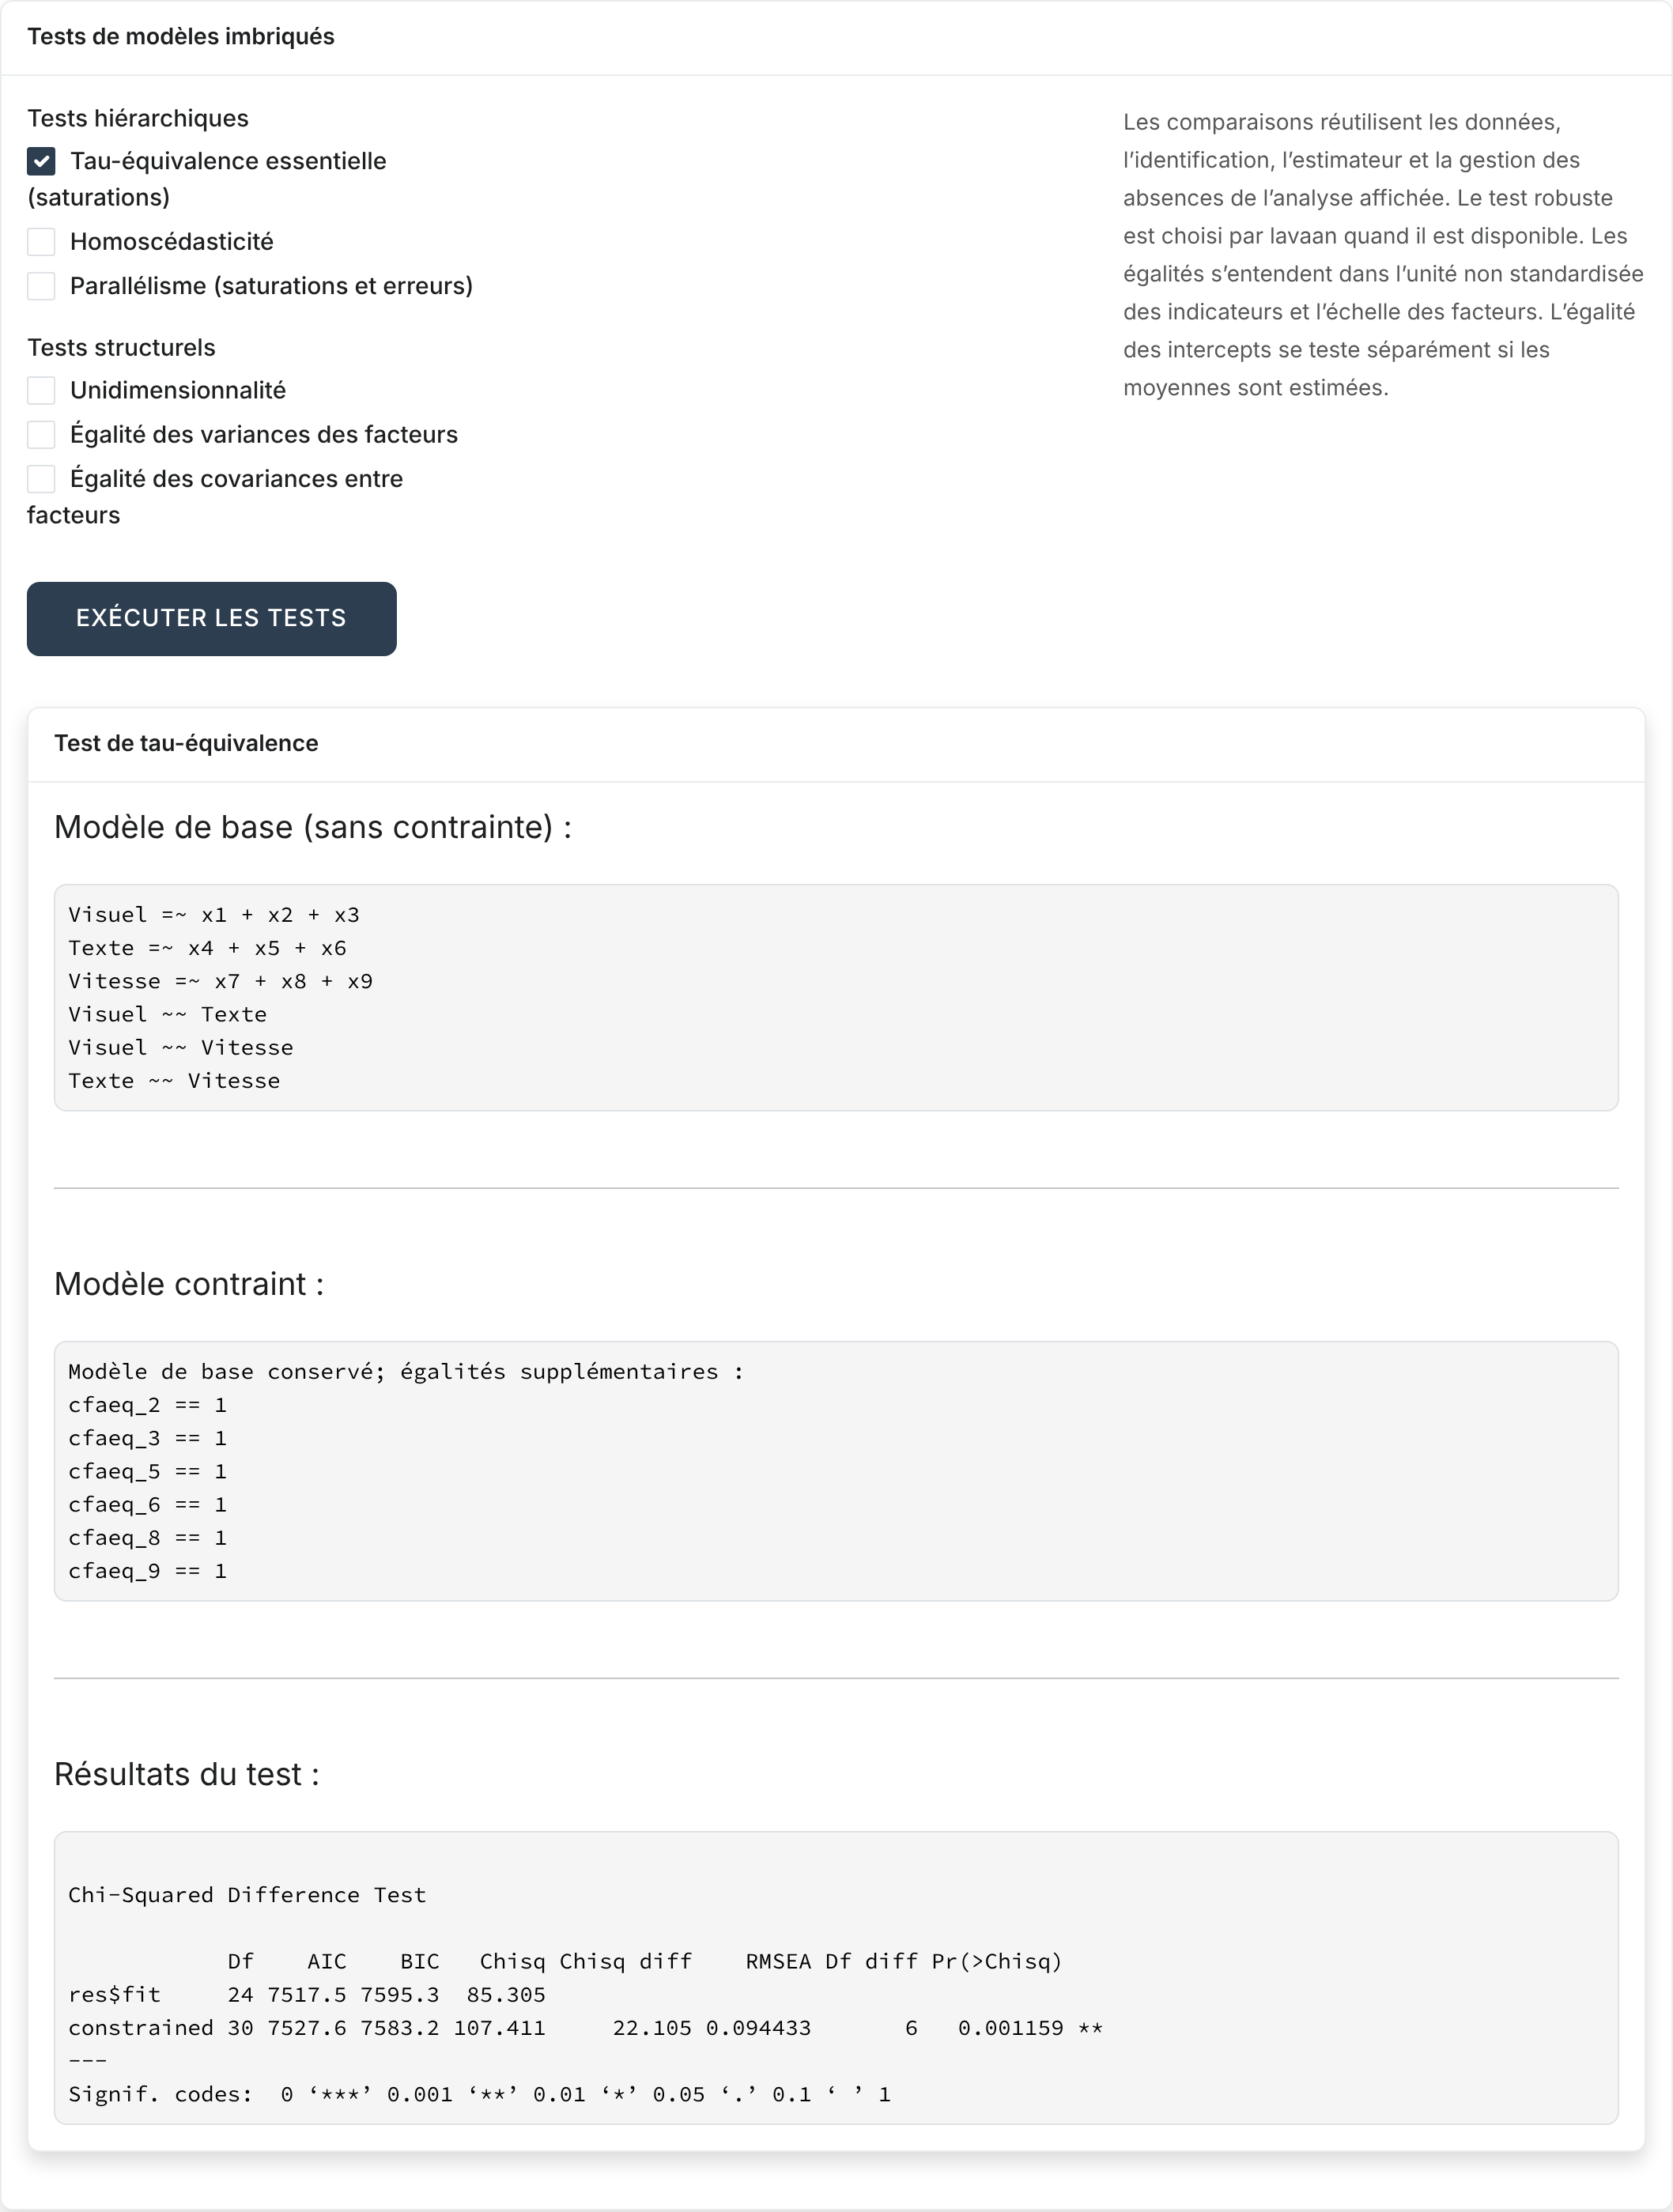
\includegraphics[width=1\linewidth,height=\textheight,keepaspectratio]{images/app/ch10_comparaisons.png}

}

\caption{\label{fig-app-comparaisons}\textbf{Analyse → Comparaisons} en
\textbf{Options avancées} : choix des tests, puis, pour chacun, le
modèle de base, les égalités ajoutées et le résultat du test de
différence.}

\end{figure}%

\Needspace{7\baselineskip}

{

\begin{longtable}[]{@{}lrrrl@{}}

\caption{\label{tbl-tests}Les trois tests hiérarchiques appliqués au
modèle HS de référence (ML, 301 élèves). Chaque ligne compare le modèle
contraint au modèle de base à 24 degrés de liberté.}

\tabularnewline

\toprule\noalign{}
Test & ddl du modèle contraint & Δχ² & Δddl & p \\
\midrule\noalign{}
\endhead
\bottomrule\noalign{}
\endlastfoot
Tau-équivalence & 30 & 22,105 & 6 & 0,001 \\
Homoscédasticité & 30 & 24,369 & 6 & \textless{} 0,001 \\
Parallélisme & 36 & 43,274 & 12 & \textless{} 0,001 \\

\end{longtable}

}

Ces résultats indiquent une dégradation détectable de l'ajustement
lorsque l'on impose ces égalités. Ils sont cohérents avec les
saturations inégales déjà observées, notamment dans le facteur visuel.
La pertinence substantielle de l'égalité reste liée aux unités des tests
cognitifs.

Avec l'identification par indicateur de référence, l'égalité des
saturations inclut la saturation fixée à 1 : elle n'est pas oubliée dans
le test. Les autres saturations doivent alors être égales à cette
référence dans l'échelle retenue. Ce n'est pas une égalité arbitraire
des seules saturations qui étaient libres. C'est pourquoi le test compte
6 degrés de liberté : deux égalités par facteur, pour trois facteurs.

\section{Lire une comparaison
imbriquée}\label{lire-une-comparaison-imbriquuxe9e}

Deux modèles sont imbriqués lorsque le modèle plus restrictif s'obtient
en ajoutant des contraintes au modèle de référence. Sous les conditions
du test, on examine la perte d'ajustement relativement au nombre de
restrictions ajoutées. Une petite valeur de p signale que les égalités
supplémentaires ne décrivent pas aussi bien les données dans ce cadre.

Avec une méthode robuste, utilisez le test de différence calculé par
l'application et sa méthode indiquée. \textbf{Ne soustrayez pas
simplement deux chi carrés corrigés.} Les corrections du test de
différence doivent être prises en compte.

Une absence de rejet ne prouve pas l'égalité exacte; la précision et la
puissance comptent. Examinez également la taille des différences et
l'intérêt de la simplification.

\section{Autres égalités et
limites}\label{autres-uxe9galituxe9s-et-limites}

L'application propose l'égalité des variances factorielles lorsqu'au
moins deux facteurs sont présents, et l'égalité des covariances
lorsqu'il existe assez de paires. Fixer déjà toutes les variances
factorielles à 1 ne laisse pas une nouvelle égalité de ces variances à
tester. Une restriction sans information nouvelle doit être signalée,
pas transformée artificiellement en résultat.

Les comparaisons automatisées d'égalité de cette version sont réservées
aux indicateurs continus. L'égalité des moyennes factorielles n'est pas
proposée comme un test ordinaire dans cette AFC à un groupe où elles
servent à l'identification. L'unidimensionnalité par corrélation
parfaite est également un cas limite; le test usuel n'est pas appliqué
automatiquement, et l'application l'explique si vous cochez
\textbf{Unidimensionnalité}.

\section{Ajouter une covariance
résiduelle}\label{ajouter-une-covariance-ruxe9siduelle}

Dans la configuration avancée, \textbf{Contraintes → Covariances} permet
de choisir deux variables, puis \textbf{Ajout}. L'objectif est de
représenter une relation résiduelle justifiée au-delà des facteurs. Par
exemple, deux tâches partageant un format de réponse pourraient
conserver une spécificité de méthode commune.

\begin{figure}[htbp]

\centering{

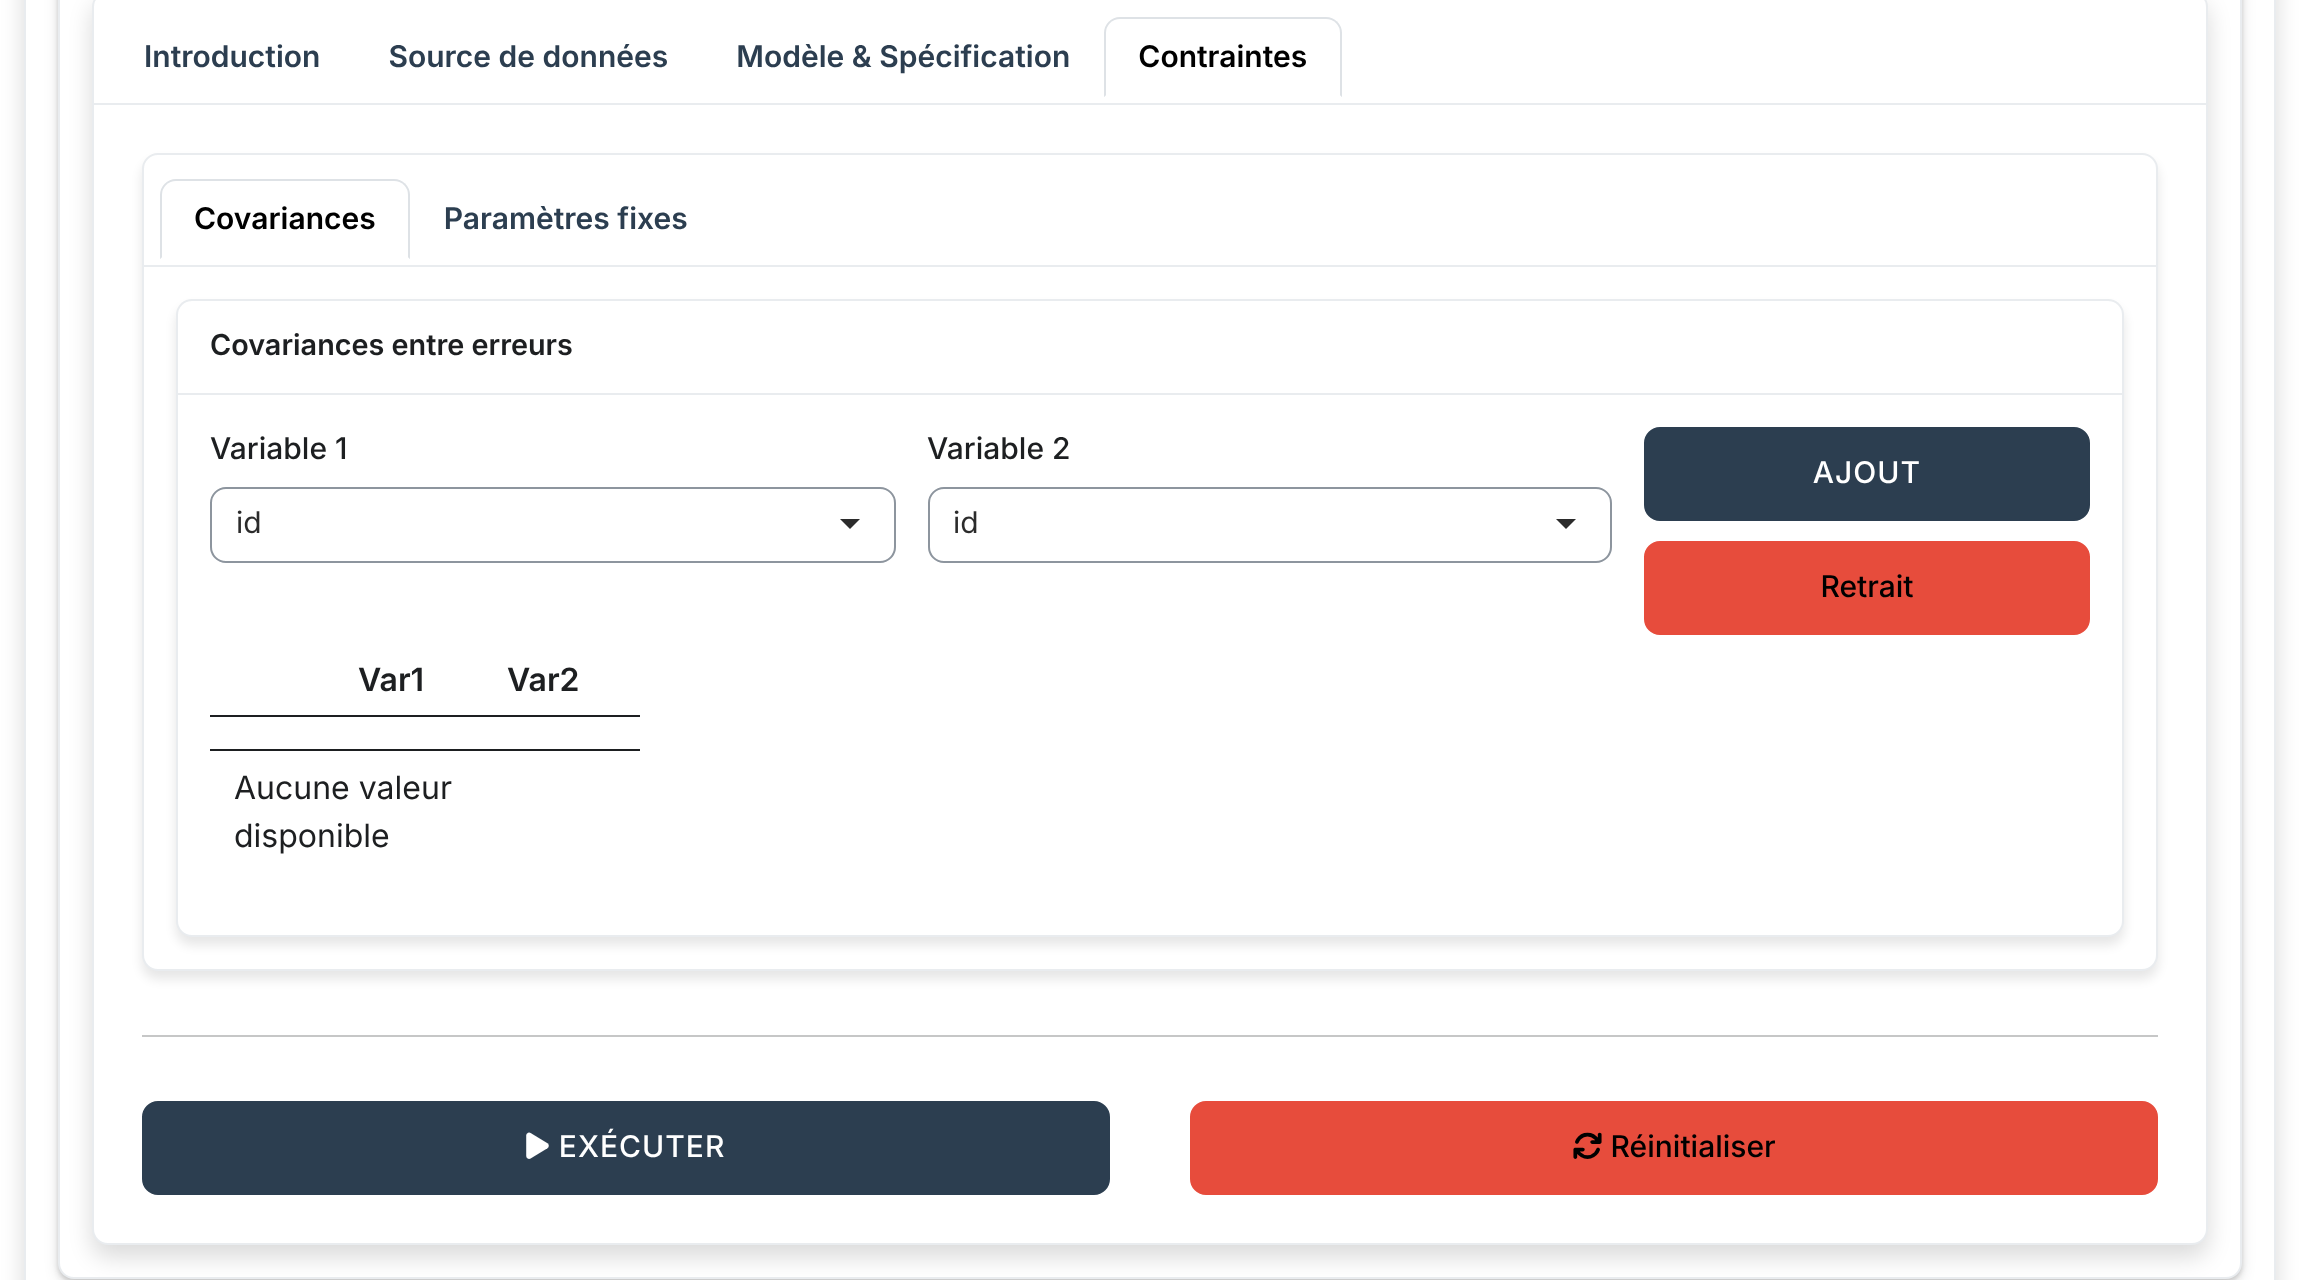
\includegraphics[width=1\linewidth,height=\textheight,keepaspectratio]{images/app/ch10_contraintes.png}

}

\caption{\label{fig-app-contraintes}\textbf{Modèle \& Spécification →
Contraintes → Covariances} : choix des deux variables, puis
\textbf{Ajout} ou \textbf{Retrait}. L'onglet \textbf{Paramètres fixes}
voisin permet de fixer ou d'étiqueter un paramètre.}

\end{figure}%

Choisissez les variables concernées, ajoutez la covariance, vérifiez la
ligne apparue, puis estimez. Ce n'est qu'après cette estimation que les
résultats et le rapport reflètent la modification. \textbf{Retrait}
permet de retirer la covariance sélectionnée pour une analyse
ultérieure.

Sur HS, ajouter \texttt{x7\ \textasciitilde{}\textasciitilde{}\ x8} fait
passer le chi carré de 85,306 à 53,272 pour un degré de liberté de moins
(différence de 32,033, p \textless{} 0,001). Le CFI passe de 0,931 à
0,966 et le RMSEA de 0,092 à 0,066. Le signal \textbf{Covariance
résiduelle} apparaît alors dans \textbf{4. Interpréter}, avec une
corrélation résiduelle de 0,471, et la saturation de \texttt{x7} sur
\texttt{Vitesse} tombe sous 0,40.

Une amélioration d'ajustement après ajout est attendue parce que le
modèle dispose d'une liberté supplémentaire. Elle ne suffit pas à
valider la justification. Documentez pourquoi cette relation a été
examinée, si elle était prévue et comment elle modifie le sens du modèle
: ici, le facteur \texttt{Vitesse} repose désormais surtout sur
\texttt{x9}, et l'oméga de la somme des trois tests baisse (chapitre sur
la fiabilité).

\section{Paramètres fixes et
étiquettes}\label{paramuxe8tres-fixes-et-uxe9tiquettes}

Le panneau \textbf{Paramètres fixes} permet de fixer un paramètre à une
valeur ou de lui donner un nom de paramètre. Réutiliser une même
étiquette peut imposer une égalité. Cette commande demande une attention
accrue : une contrainte posée sur un mauvais facteur ou dans une échelle
mal comprise change réellement le modèle.

Pour la première utilisation, limitez-vous à une restriction dont vous
pouvez écrire le sens en français. Si vous ne pouvez pas expliquer
l'égalité souhaitée avant le clic, ne l'ajoutez pas pour améliorer
seulement un indice.

\section{Laboratoire : tau-équivalence et
fiabilité}\label{laboratoire-tau-uxe9quivalence-et-fiabilituxe9}

Comparez le modèle HS de référence et sa version tau-équivalente.
Consignez l'hypothèse, les degrés de liberté, le test de différence, la
méthode et la conclusion. Expliquez ensuite pourquoi l'obtention de
meilleures valeurs de fiabilité dans un modèle contraint ne justifierait
pas de retenir ce modèle si ses restrictions étaient mal soutenues.

\begin{tcolorbox}[enhanced jigsaw, arc=.35mm, bottomrule=.15mm, bottomtitle=1mm, breakable, colback=white, colbacktitle=quarto-callout-tip-color!10!white, colframe=quarto-callout-tip-color-frame, coltitle=black, left=2mm, leftrule=.75mm, opacityback=0, opacitybacktitle=0.6, rightrule=.15mm, title={Réponse}, titlerule=0mm, toprule=.15mm, toptitle=1mm]

Hypothèse : au sein de chaque facteur, les trois tests ont la même
saturation non standardisée (égale à celle de l'indicateur de
référence). Le modèle contraint a 30 degrés de liberté contre 24; la
différence de chi carré vaut 22,105 pour 6 dl, p = 0,0012 (ML, test
usuel). Les données ne soutiennent pas l'égalité des saturations : les
tests contribuent inégalement à leur facteur, ce que montraient déjà les
saturations standardisées.

Un modèle contraint peut afficher une fiabilité différente parce que ses
paramètres sont imposés, pas parce que la mesure est meilleure. Si la
restriction est rejetée par les données, ses indices décrivent un modèle
qui ne représente pas bien les tests : les citer reviendrait à choisir
le modèle pour son résultat.

\end{tcolorbox}

\begin{tcolorbox}[enhanced jigsaw, arc=.35mm, bottomrule=.15mm, bottomtitle=1mm, breakable, colback=white, colbacktitle=quarto-callout-important-color!10!white, colframe=quarto-callout-important-color-frame, coltitle=black, left=2mm, leftrule=.75mm, opacityback=0, opacitybacktitle=0.6, rightrule=.15mm, title={À retenir}, titlerule=0mm, toprule=.15mm, toptitle=1mm]

\begin{itemize}
\tightlist
\item
  Les égalités testées portent sur les paramètres non standardisés, dans
  l'échelle choisie.
\item
  Un test de différence compare deux modèles imbriqués estimés sur les
  mêmes données et avec la même méthode.
\item
  Avec un estimateur robuste, on utilise le test de différence corrigé,
  pas une soustraction.
\item
  Une covariance résiduelle améliore toujours l'ajustement : sa
  justification doit précéder son ajout.
\end{itemize}

\end{tcolorbox}

\section{Quiz}\label{quiz-9}

\begin{enumerate}
\def\labelenumi{\arabic{enumi}.}
\tightlist
\item
  Pourquoi la tau-équivalence ajoute-t-elle six degrés de liberté au
  modèle HS ?
\item
  Le test de tau-équivalence n'est pas significatif. Les saturations
  sont-elles égales ?
\item
  Peut-on tester l'égalité des variances factorielles avec
  l'identification σ²(F)=1 ?
\item
  Après l'ajout de \texttt{x7\ \textasciitilde{}\textasciitilde{}\ x8},
  le CFI s'améliore. Est-ce une preuve que la covariance existe ?
\end{enumerate}

\begin{tcolorbox}[enhanced jigsaw, arc=.35mm, bottomrule=.15mm, bottomtitle=1mm, breakable, colback=white, colbacktitle=quarto-callout-tip-color!10!white, colframe=quarto-callout-tip-color-frame, coltitle=black, left=2mm, leftrule=.75mm, opacityback=0, opacitybacktitle=0.6, rightrule=.15mm, title={Réponses}, titlerule=0mm, toprule=.15mm, toptitle=1mm]

\begin{enumerate}
\def\labelenumi{\arabic{enumi}.}
\tightlist
\item
  Chaque facteur a trois saturations; les rendre égales impose deux
  égalités par facteur, soit six pour trois facteurs.
\item
  Non. Les données ne permettent pas de rejeter l'égalité; la puissance
  et la taille des écarts restent à discuter.
\item
  Non : les variances sont déjà toutes fixées à 1, la restriction
  n'ajoute aucune information.
\item
  Non. Toute liberté ajoutée améliore l'ajustement; il faut une
  justification de contenu et, idéalement, une réplication.
\end{enumerate}

\end{tcolorbox}

\bookmarksetup{startatroot}

\chapter{Utiliser la simulation pour comprendre le
modèle}\label{sec-simulation}

\begin{tcolorbox}[enhanced jigsaw, arc=.35mm, bottomrule=.15mm, bottomtitle=1mm, breakable, colback=white, colbacktitle=quarto-callout-note-color!10!white, colframe=quarto-callout-note-color-frame, coltitle=black, left=2mm, leftrule=.75mm, opacityback=0, opacitybacktitle=0.6, rightrule=.15mm, title={Objectifs du chapitre}, titlerule=0mm, toprule=.15mm, toptitle=1mm]

\begin{itemize}
\tightlist
\item
  Distinguer les paramètres fixés dans la population, les valeurs tirées
  et les estimations.
\item
  Reproduire un échantillon grâce à la graine.
\item
  Observer l'effet de l'effectif et de la force des indicateurs sur les
  estimations.
\item
  Créer délibérément une mauvaise spécification et en observer les
  conséquences.
\end{itemize}

\end{tcolorbox}

\begin{tcolorbox}[enhanced jigsaw, arc=.35mm, bottomrule=.15mm, bottomtitle=1mm, breakable, colback=white, colbacktitle=quarto-callout-tip-color!10!white, colframe=quarto-callout-tip-color-frame, coltitle=black, left=2mm, leftrule=.75mm, opacityback=0, opacitybacktitle=0.6, rightrule=.15mm, title={Idée centrale}, titlerule=0mm, toprule=.15mm, toptitle=1mm]

Avec des données réelles, on ne connaît jamais la bonne réponse. Avec
une simulation, on la fixe d'avance : on peut alors voir de combien une
estimation s'en écarte d'un échantillon à l'autre et comment un indice
réagit à un défaut qu'on a introduit soi-même.

\end{tcolorbox}

\section{Une population connue et un échantillon
variable}\label{une-population-connue-et-un-uxe9chantillon-variable}

Les données réelles ne donnent pas directement accès aux paramètres de
la population. La simulation permet de définir ces paramètres puis de
générer un échantillon. Elle aide à comprendre les fluctuations
d'estimation, la force des indicateurs et les conséquences d'une
mauvaise spécification.

Les paramètres de simulation ne constituent pas les résultats de l'AFC.
Une saturation demandée à 0,70 dans la population ne sera pas exactement
estimée à 0,70 dans chaque échantillon. C'est précisément l'un des
intérêts pédagogiques de l'expérience.

\section{Préparer une première expérience
contrôlée}\label{pruxe9parer-une-premiuxe8re-expuxe9rience-contruxf4luxe9e}

Dans \textbf{1. Choisir les données → Données simulées}, fixez : un
facteur, quatre indicateurs, 100 observations, données continues. Dans
\textbf{Force des loadings}, placez les deux bornes à \textbf{0,70}.
Avec un seul facteur, l'étendue des corrélations entre facteurs
n'intervient pas.

\begin{figure}[htbp]

\centering{

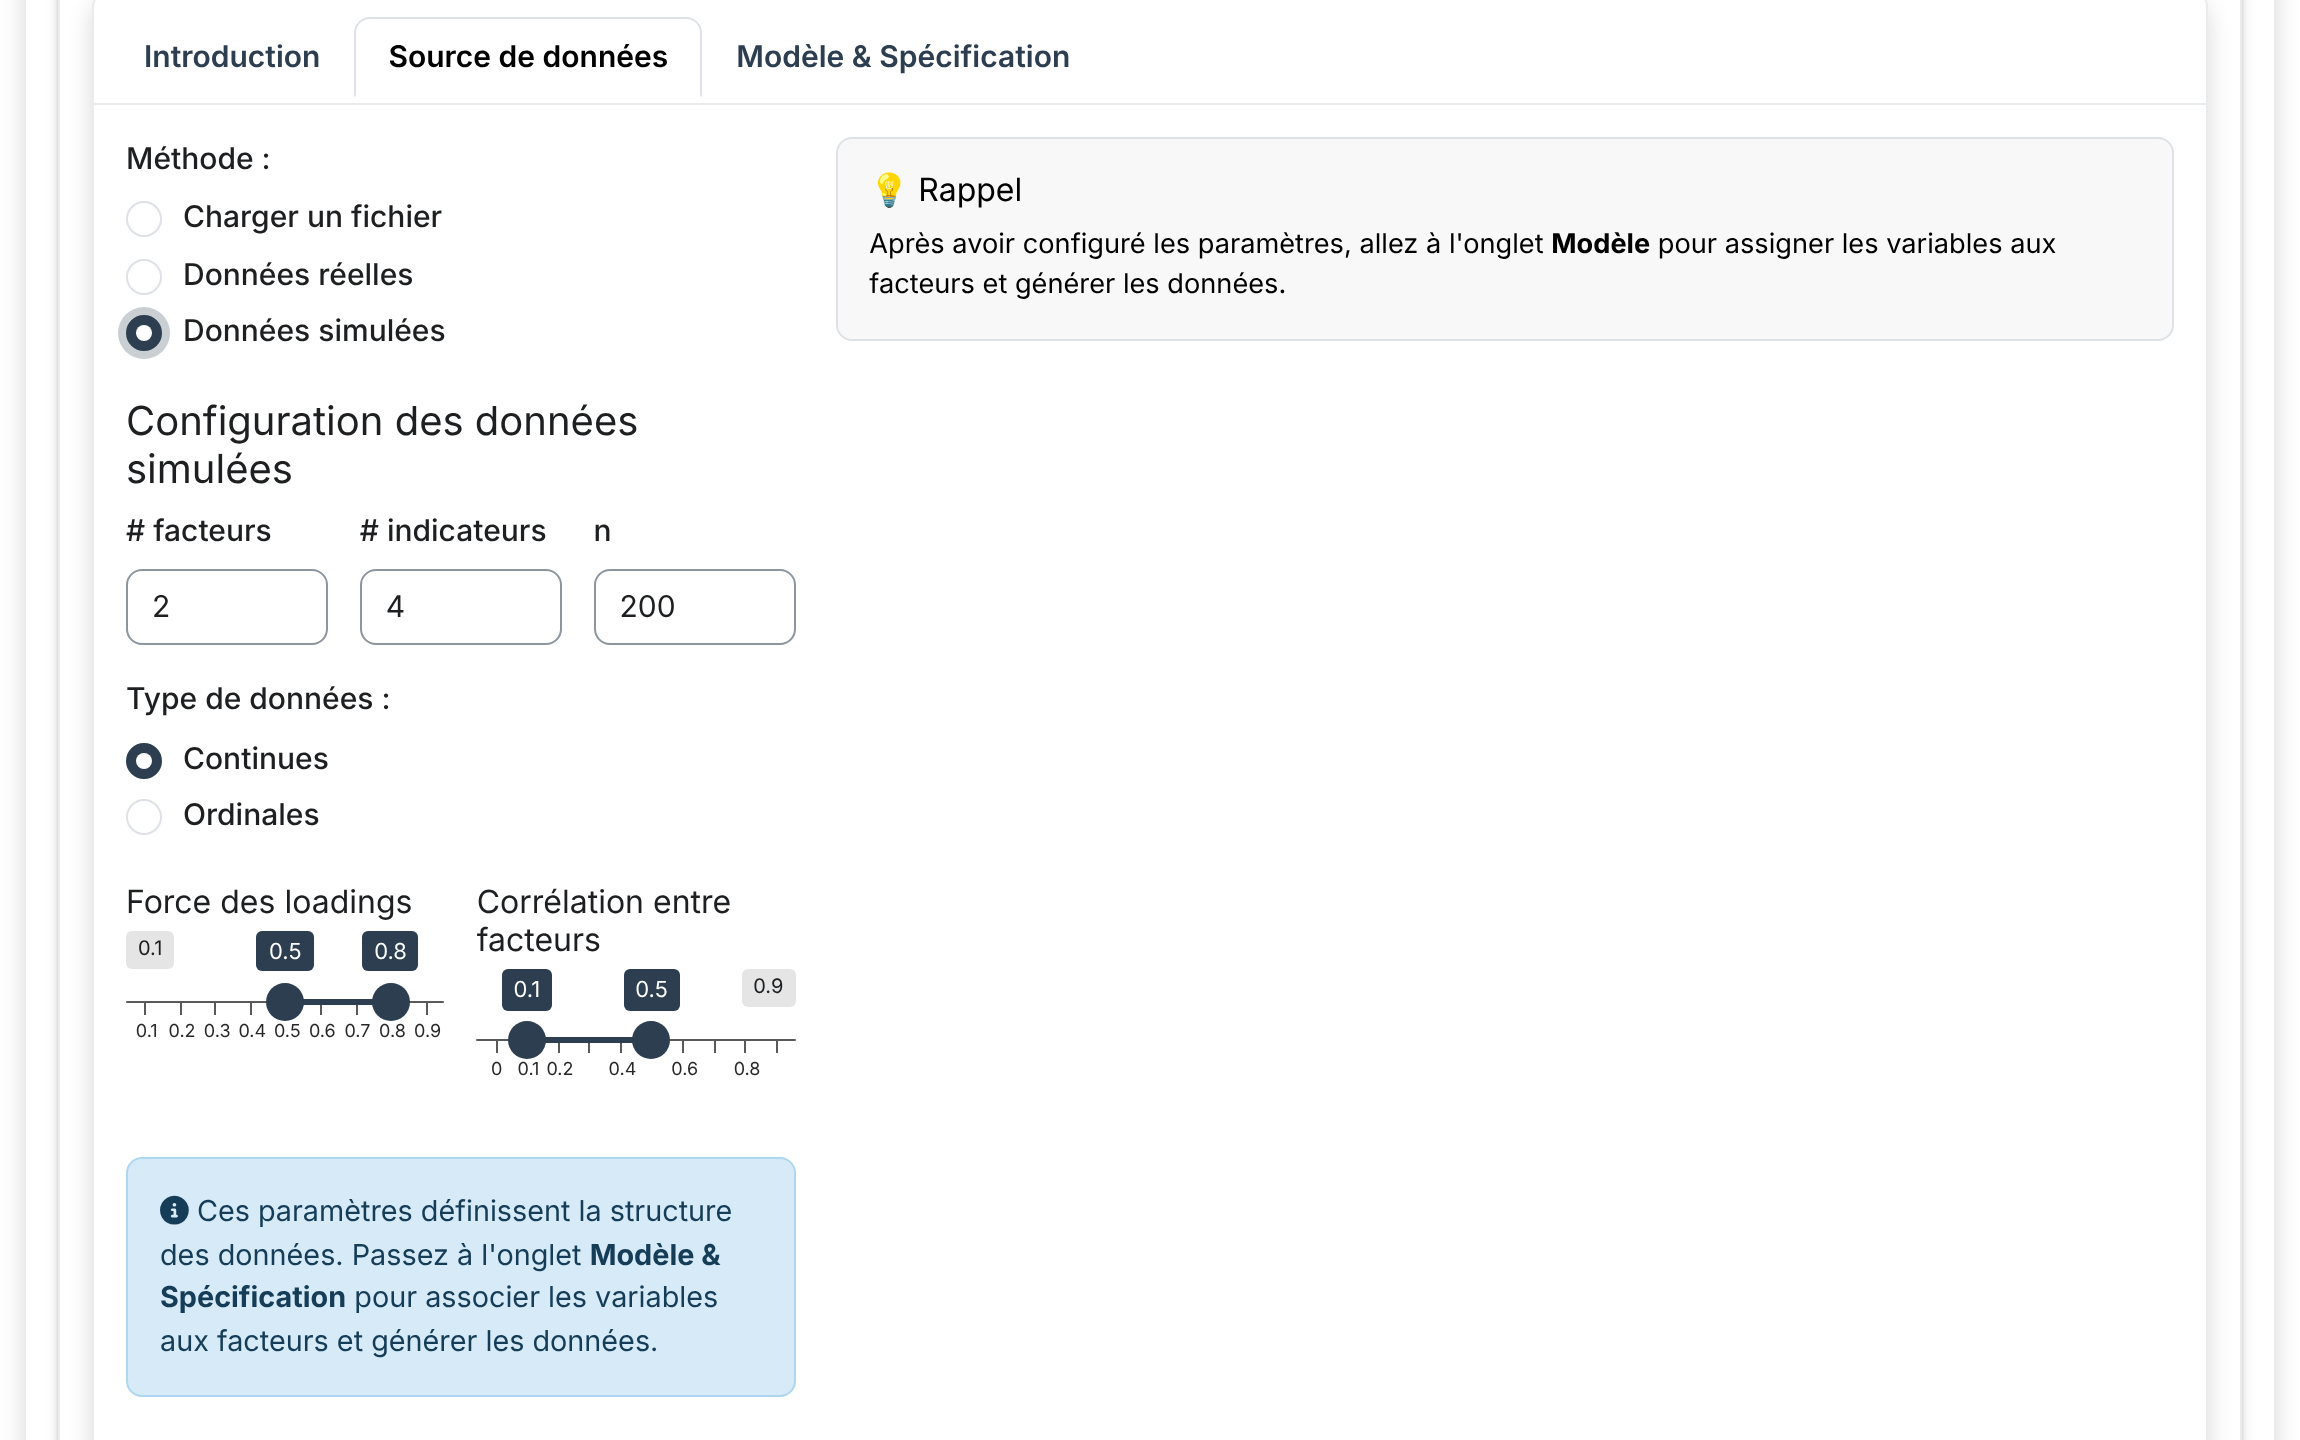
\includegraphics[width=1\linewidth,height=\textheight,keepaspectratio]{images/app/ch11_simulation.png}

}

\caption{\label{fig-app-simulation}\textbf{Source de données → Données
simulées} : nombre de facteurs et d'indicateurs, effectif, type de
données, étendue des saturations (« Force des loadings ») et des
corrélations entre facteurs.}

\end{figure}%

Passez à \textbf{2. Définir le modèle}. Vérifiez le facteur \texttt{F1}
et les variables \texttt{x1}, \texttt{x2}, \texttt{x3}, \texttt{x4}.
Dans le bloc de génération, saisissez la \textbf{graine 123}, puis
cliquez sur \textbf{Générer les données}. Choisissez ML, les cas
complets et l'indicateur de référence; estimez.

Si vous ne parvenez pas à superposer exactement les deux poignées du
curseur, vérifiez les valeurs affichées aux extrémités. Une étendue
proche de 0,70 mais non égale génère des saturations de population
différentes de celles de cette expérience de référence.

\section{Ce que signifie la graine}\label{ce-que-signifie-la-graine}

La graine fixe le point de départ du générateur aléatoire. Avec les
mêmes réglages et le même environnement, elle permet de reproduire
l'échantillon. \textbf{La valeur 0 est une graine fixe dans cette
application; elle ne signifie pas « au hasard ».}

Changer la graine produit un autre échantillon et peut aussi changer les
paramètres tirés dans les étendues demandées. Pour isoler un effet,
conservez les autres réglages et utilisez des étendues ponctuelles
lorsque c'est possible.

\section{Variance expliquée d'un
indicateur}\label{variance-expliquuxe9e-dun-indicateur}

Avec une saturation de population standardisée de 0,70, la variance
expliquée de chaque indicateur simple est de 0,49 et la part résiduelle
de 0,51. Les saturations demandées dans l'application sont standardisées
dans la population; les résidus sont générés en cohérence avec cette
définition.

\begin{figure}[htbp]

\centering{

\includegraphics[width=0.88\linewidth,height=\textheight,keepaspectratio]{11-simulation_files/figure-pdf/fig-variance-expliquee-1.png}

}

\caption{\label{fig-variance-expliquee}Variance expliquée d'un
indicateur (carré de la saturation standardisée) et oméga de la somme de
quatre indicateurs équivalents, en fonction de la saturation de
population. Les points marquent les trois conditions de l'expérience sur
la force des indicateurs.}

\end{figure}%

Passer d'une saturation de 0,40 à 0,70 n'ajoute pas seulement 0,30 à la
proportion expliquée : celle-ci passe de 0,16 à 0,49. Cela aide à
comprendre pourquoi des indicateurs assez faiblement reliés au facteur
peuvent limiter fortement la qualité d'un score.

\section{Augmenter l'effectif}\label{augmenter-leffectif}

Conservez les mêmes réglages, passez à \textbf{1 000 observations},
régénérez les données avec la graine 123 et estimez de nouveau. Notez
les saturations et les erreurs-types. Ne vous contentez pas de comparer
les valeurs de p, qui dépendent fortement de l'effectif.

Voici deux repères pour cette expérience précise :

\Needspace{7\baselineskip}

{

\begin{longtable}[]{@{}lrrr@{}}

\caption{\label{tbl-sim}Oméga et AVE estimés dans les deux échantillons
(graine 123), comparés à leurs valeurs de population. Erreur-type :
moyenne des erreurs-types des saturations libres.}

\tabularnewline

\toprule\noalign{}
Échantillon & Oméga & AVE & Erreur-type moyenne \\
\midrule\noalign{}
\endhead
\bottomrule\noalign{}
\endlastfoot
100 observations & 0,769 & 0,453 & 0,253 \\
1 000 observations & 0,811 & 0,518 & 0,052 \\
Population & 0,794 & 0,490 & --- \\

\end{longtable}

}

Dans cette population, l'AVE vaut 0,49 et l'oméga de la somme vaut
0,794. Les estimations échantillonnales fluctuent autour de ces cibles.
L'erreur-type moyenne des saturations passe de 0,253 à 0,052, soit à peu
près une division par \(\sqrt{10}\approx 3{,}2\). Un échantillon plus
grand ne garantit pas que chaque paramètre sera, lors d'un tirage
particulier, plus proche de la population; il réduit généralement la
variabilité d'estimation dans des répétitions comparables.

\begin{figure}[htbp]

\centering{

\includegraphics[width=0.88\linewidth,height=\textheight,keepaspectratio]{11-simulation_files/figure-pdf/fig-sim-mc-1.png}

}

\caption{\label{fig-sim-mc}Oméga estimé dans 200 échantillons simulés de
chaque taille (même population : un facteur, quatre saturations de 0,70;
graines 1001 à 1200). La ligne verticale marque la valeur de population.
Avec 100 observations, une part non négligeable des échantillons tombe
sous 0,70.}

\end{figure}%

Sur 200 répétitions, l'oméga estimé varie de 0,66 à 0,88 avec 100
observations, et de 0,76 à 0,82 avec 1 000. Avec 100 observations, 1~\%
des échantillons donnent un oméga sous 0,70, alors que la valeur de
population est 0,79. Un repère appliqué à une seule estimation peut donc
conduire à des conclusions opposées pour une même population.

Les données de 100 observations ne doivent pas être considérées
automatiquement comme les 100 premières lignes des données de 1 000
observations. La procédure de génération peut organiser les tirages
différemment selon la dimension de l'échantillon. Comparez les
conditions et les résultats, sans supposer un emboîtement des lignes.

\section{Augmenter la force des
indicateurs}\label{augmenter-la-force-des-indicateurs}

Avec 1 000 observations et quatre indicateurs, comparez trois conditions
: saturations fixées à 0,40, puis 0,70, puis 0,90. Conservez la graine
123, régénérez à chaque condition et estimez. La population simple
prévoit une AVE de 0,16, 0,49 et 0,81 respectivement.

\Needspace{7\baselineskip}

{

\begin{longtable}[]{@{}
  >{\raggedleft\arraybackslash}p{(\linewidth - 8\tabcolsep) * \real{0.1618}}
  >{\raggedleft\arraybackslash}p{(\linewidth - 8\tabcolsep) * \real{0.2206}}
  >{\raggedleft\arraybackslash}p{(\linewidth - 8\tabcolsep) * \real{0.1765}}
  >{\raggedleft\arraybackslash}p{(\linewidth - 8\tabcolsep) * \real{0.2500}}
  >{\raggedleft\arraybackslash}p{(\linewidth - 8\tabcolsep) * \real{0.1912}}@{}}

\caption{\label{tbl-force}Effet de la force des indicateurs (1 000
observations, graine 123) : valeurs de population et estimations.}

\tabularnewline

\toprule\noalign{}
\begin{minipage}[b]{\linewidth}\raggedleft
Saturation
\end{minipage} & \begin{minipage}[b]{\linewidth}\raggedleft
AVE population
\end{minipage} & \begin{minipage}[b]{\linewidth}\raggedleft
AVE estimée
\end{minipage} & \begin{minipage}[b]{\linewidth}\raggedleft
Oméga population
\end{minipage} & \begin{minipage}[b]{\linewidth}\raggedleft
Oméga estimé
\end{minipage} \\
\midrule\noalign{}
\endhead
\bottomrule\noalign{}
\endlastfoot
0,400 & 0,160 & 0,189 & 0,432 & 0,481 \\
0,700 & 0,490 & 0,518 & 0,794 & 0,811 \\
0,900 & 0,810 & 0,824 & 0,945 & 0,949 \\

\end{longtable}

}

L'oméga de la somme de quatre indicateurs équivalents vaut 0,432, 0,794
et 0,945 dans ces trois conditions de population. Cette augmentation
découle de la structure de population définie; il ne s'agit pas d'un
effet à attribuer à un nouvel instrument réel.

\section{Simuler deux facteurs}\label{simuler-deux-facteurs}

Choisissez deux facteurs et six indicateurs. La population générée
répartit automatiquement les trois premiers indicateurs dans \texttt{F1}
et les trois suivants dans \texttt{F2}. Lisez l'avertissement de
l'application : modifier ensuite les affectations du modèle analysé ne
change pas silencieusement cette population de génération.

Pour étudier une mauvaise spécification, générez les données sous cette
répartition, puis attribuez par exemple \texttt{x3} au second facteur
dans le modèle analysé. Comparez l'ajustement et les saturations. Vous
avez délibérément fait diverger le modèle estimé du modèle générateur;
cette différence doit être annoncée.

Des corrélations factorielles élevées peuvent rendre les distinctions
plus difficiles. Avec plus de deux facteurs, toutes les combinaisons de
corrélations ne forment pas une matrice admissible. Si une étendue
demandée ne permet pas une génération valable, l'application le signale;
réduisez-la plutôt que de supposer que le logiciel réparera les
relations sans vous le dire.

\section{Simuler des réponses
ordinales}\label{simuler-des-ruxe9ponses-ordinales}

Le choix \textbf{Ordinales} transforme les réponses latentes en
catégories d'effectifs à peu près égaux. Vérifiez le nombre de
catégories, régénérez les données et utilisez les déclarations ordinales
ainsi que WLSMV pour l'estimation. L'objectif est d'observer la relation
entre catégories et modèle sous-jacent, pas de forcer les catégories à
passer un test continu de normalité.

\section{Laboratoire : une mauvaise spécification
volontaire}\label{laboratoire-une-mauvaise-spuxe9cification-volontaire}

\begin{enumerate}
\def\labelenumi{\arabic{enumi}.}
\tightlist
\item
  Simulez deux facteurs, six indicateurs, 500 observations, données
  continues, saturations de 0,70 à 0,70 et corrélation entre facteurs de
  0,30 à 0,30, avec la graine 42.
\item
  Estimez d'abord le modèle correct (\texttt{x1}--\texttt{x3} sur
  \texttt{F1}, \texttt{x4}--\texttt{x6} sur \texttt{F2}) et relevez le
  CFI, le RMSEA et la saturation standardisée de \texttt{x3}.
\item
  Déplacez \texttt{x3} vers \texttt{F2}, estimez de nouveau et relevez
  les mêmes valeurs.
\item
  Quels diagnostics signalent le problème ? Lesquels restent silencieux
  ?
\end{enumerate}

\begin{tcolorbox}[enhanced jigsaw, arc=.35mm, bottomrule=.15mm, bottomtitle=1mm, breakable, colback=white, colbacktitle=quarto-callout-tip-color!10!white, colframe=quarto-callout-tip-color-frame, coltitle=black, left=2mm, leftrule=.75mm, opacityback=0, opacitybacktitle=0.6, rightrule=.15mm, title={Réponse}, titlerule=0mm, toprule=.15mm, toptitle=1mm]

Le modèle correct s'ajuste très bien (CFI 1,000, RMSEA 0,000) et
\texttt{x3} sature à 0,722 sur \texttt{F1}. Placé sur \texttt{F2},
\texttt{x3} n'y sature plus qu'à 0,200, et l'ajustement se dégrade (CFI
0,726, RMSEA 0,219). Les signaux de l'application relèvent charge faible
et peu d'indicateurs : ils pointent le bon indicateur. \texttt{F1},
réduit à deux indicateurs, devient aussi plus fragile. Une mauvaise
affectation se voit surtout dans l'ajustement, les résidus et les
indices de modification.

\end{tcolorbox}

\begin{tcolorbox}[enhanced jigsaw, arc=.35mm, bottomrule=.15mm, bottomtitle=1mm, breakable, colback=white, colbacktitle=quarto-callout-important-color!10!white, colframe=quarto-callout-important-color-frame, coltitle=black, left=2mm, leftrule=.75mm, opacityback=0, opacitybacktitle=0.6, rightrule=.15mm, title={À retenir}, titlerule=0mm, toprule=.15mm, toptitle=1mm]

\begin{itemize}
\tightlist
\item
  Les paramètres de simulation sont la vérité de la population; les
  estimations fluctuent autour.
\item
  La graine rend un tirage reproductible; 0 est une graine comme une
  autre.
\item
  L'erreur-type diminue environ comme \(1/\sqrt{n}\); la fiabilité d'un
  score dépend surtout de la force et du nombre des indicateurs.
\item
  Une estimation isolée comparée à un seuil peut mener à des conclusions
  opposées pour une même population.
\end{itemize}

\end{tcolorbox}

\section{Quiz}\label{quiz-10}

\begin{enumerate}
\def\labelenumi{\arabic{enumi}.}
\tightlist
\item
  La saturation demandée vaut 0,70 et l'estimation vaut 0,74.
  L'application s'est-elle trompée ?
\item
  Pourquoi l'oméga de quatre indicateurs à 0,70 dépasse-t-il nettement
  la variance expliquée de chacun ?
\item
  Vous modifiez l'affectation des indicateurs après la génération. La
  population change-t-elle ?
\item
  Pourquoi choisir des étendues ponctuelles (bornes égales) pour une
  expérience ?
\end{enumerate}

\begin{tcolorbox}[enhanced jigsaw, arc=.35mm, bottomrule=.15mm, bottomtitle=1mm, breakable, colback=white, colbacktitle=quarto-callout-tip-color!10!white, colframe=quarto-callout-tip-color-frame, coltitle=black, left=2mm, leftrule=.75mm, opacityback=0, opacitybacktitle=0.6, rightrule=.15mm, title={Réponses}, titlerule=0mm, toprule=.15mm, toptitle=1mm]

\begin{enumerate}
\def\labelenumi{\arabic{enumi}.}
\tightlist
\item
  Non. C'est une fluctuation d'échantillonnage autour de la valeur de
  population.
\item
  Parce que la somme accumule la variance commune plus vite que la
  variance propre des indicateurs.
\item
  Non. Seul le modèle estimé change; la population reste celle de la
  génération.
\item
  Pour que seuls les réglages étudiés changent d'une condition à
  l'autre, et pas les saturations tirées.
\end{enumerate}

\end{tcolorbox}

\bookmarksetup{startatroot}

\chapter{Conserver et communiquer une analyse}\label{sec-rapport}

\begin{tcolorbox}[enhanced jigsaw, arc=.35mm, bottomrule=.15mm, bottomtitle=1mm, breakable, colback=white, colbacktitle=quarto-callout-note-color!10!white, colframe=quarto-callout-note-color-frame, coltitle=black, left=2mm, leftrule=.75mm, opacityback=0, opacitybacktitle=0.6, rightrule=.15mm, title={Objectifs du chapitre}, titlerule=0mm, toprule=.15mm, toptitle=1mm]

\begin{itemize}
\tightlist
\item
  Exporter des scores factoriels en conservant la correspondance avec
  les personnes.
\item
  Comprendre pourquoi les scores ne reproduisent pas exactement les
  corrélations entre facteurs.
\item
  Préparer un diagramme et un rapport qui décrivent la bonne analyse.
\item
  Structurer une présentation écrite reproductible.
\end{itemize}

\end{tcolorbox}

\begin{tcolorbox}[enhanced jigsaw, arc=.35mm, bottomrule=.15mm, bottomtitle=1mm, breakable, colback=white, colbacktitle=quarto-callout-tip-color!10!white, colframe=quarto-callout-tip-color-frame, coltitle=black, left=2mm, leftrule=.75mm, opacityback=0, opacitybacktitle=0.6, rightrule=.15mm, title={Idée centrale}, titlerule=0mm, toprule=.15mm, toptitle=1mm]

Un score factoriel est une \textbf{prédiction}, pas une mesure du
facteur. Un rapport n'est utile que s'il décrit exactement l'analyse
enregistrée : données, modèle, estimateur, effectif et versions des
indices.

\end{tcolorbox}

\section{Les scores factoriels sont des
estimations}\label{les-scores-factoriels-sont-des-estimations}

Dans \textbf{Analyse → Suppléments → Scores factoriels}, l'application
propose \textbf{Régression} et \textbf{Bartlett}, selon la compatibilité
avec le modèle et l'estimateur. Commencez avec les données continues HS
et la méthode Régression.

\begin{figure}[htbp]

\centering{

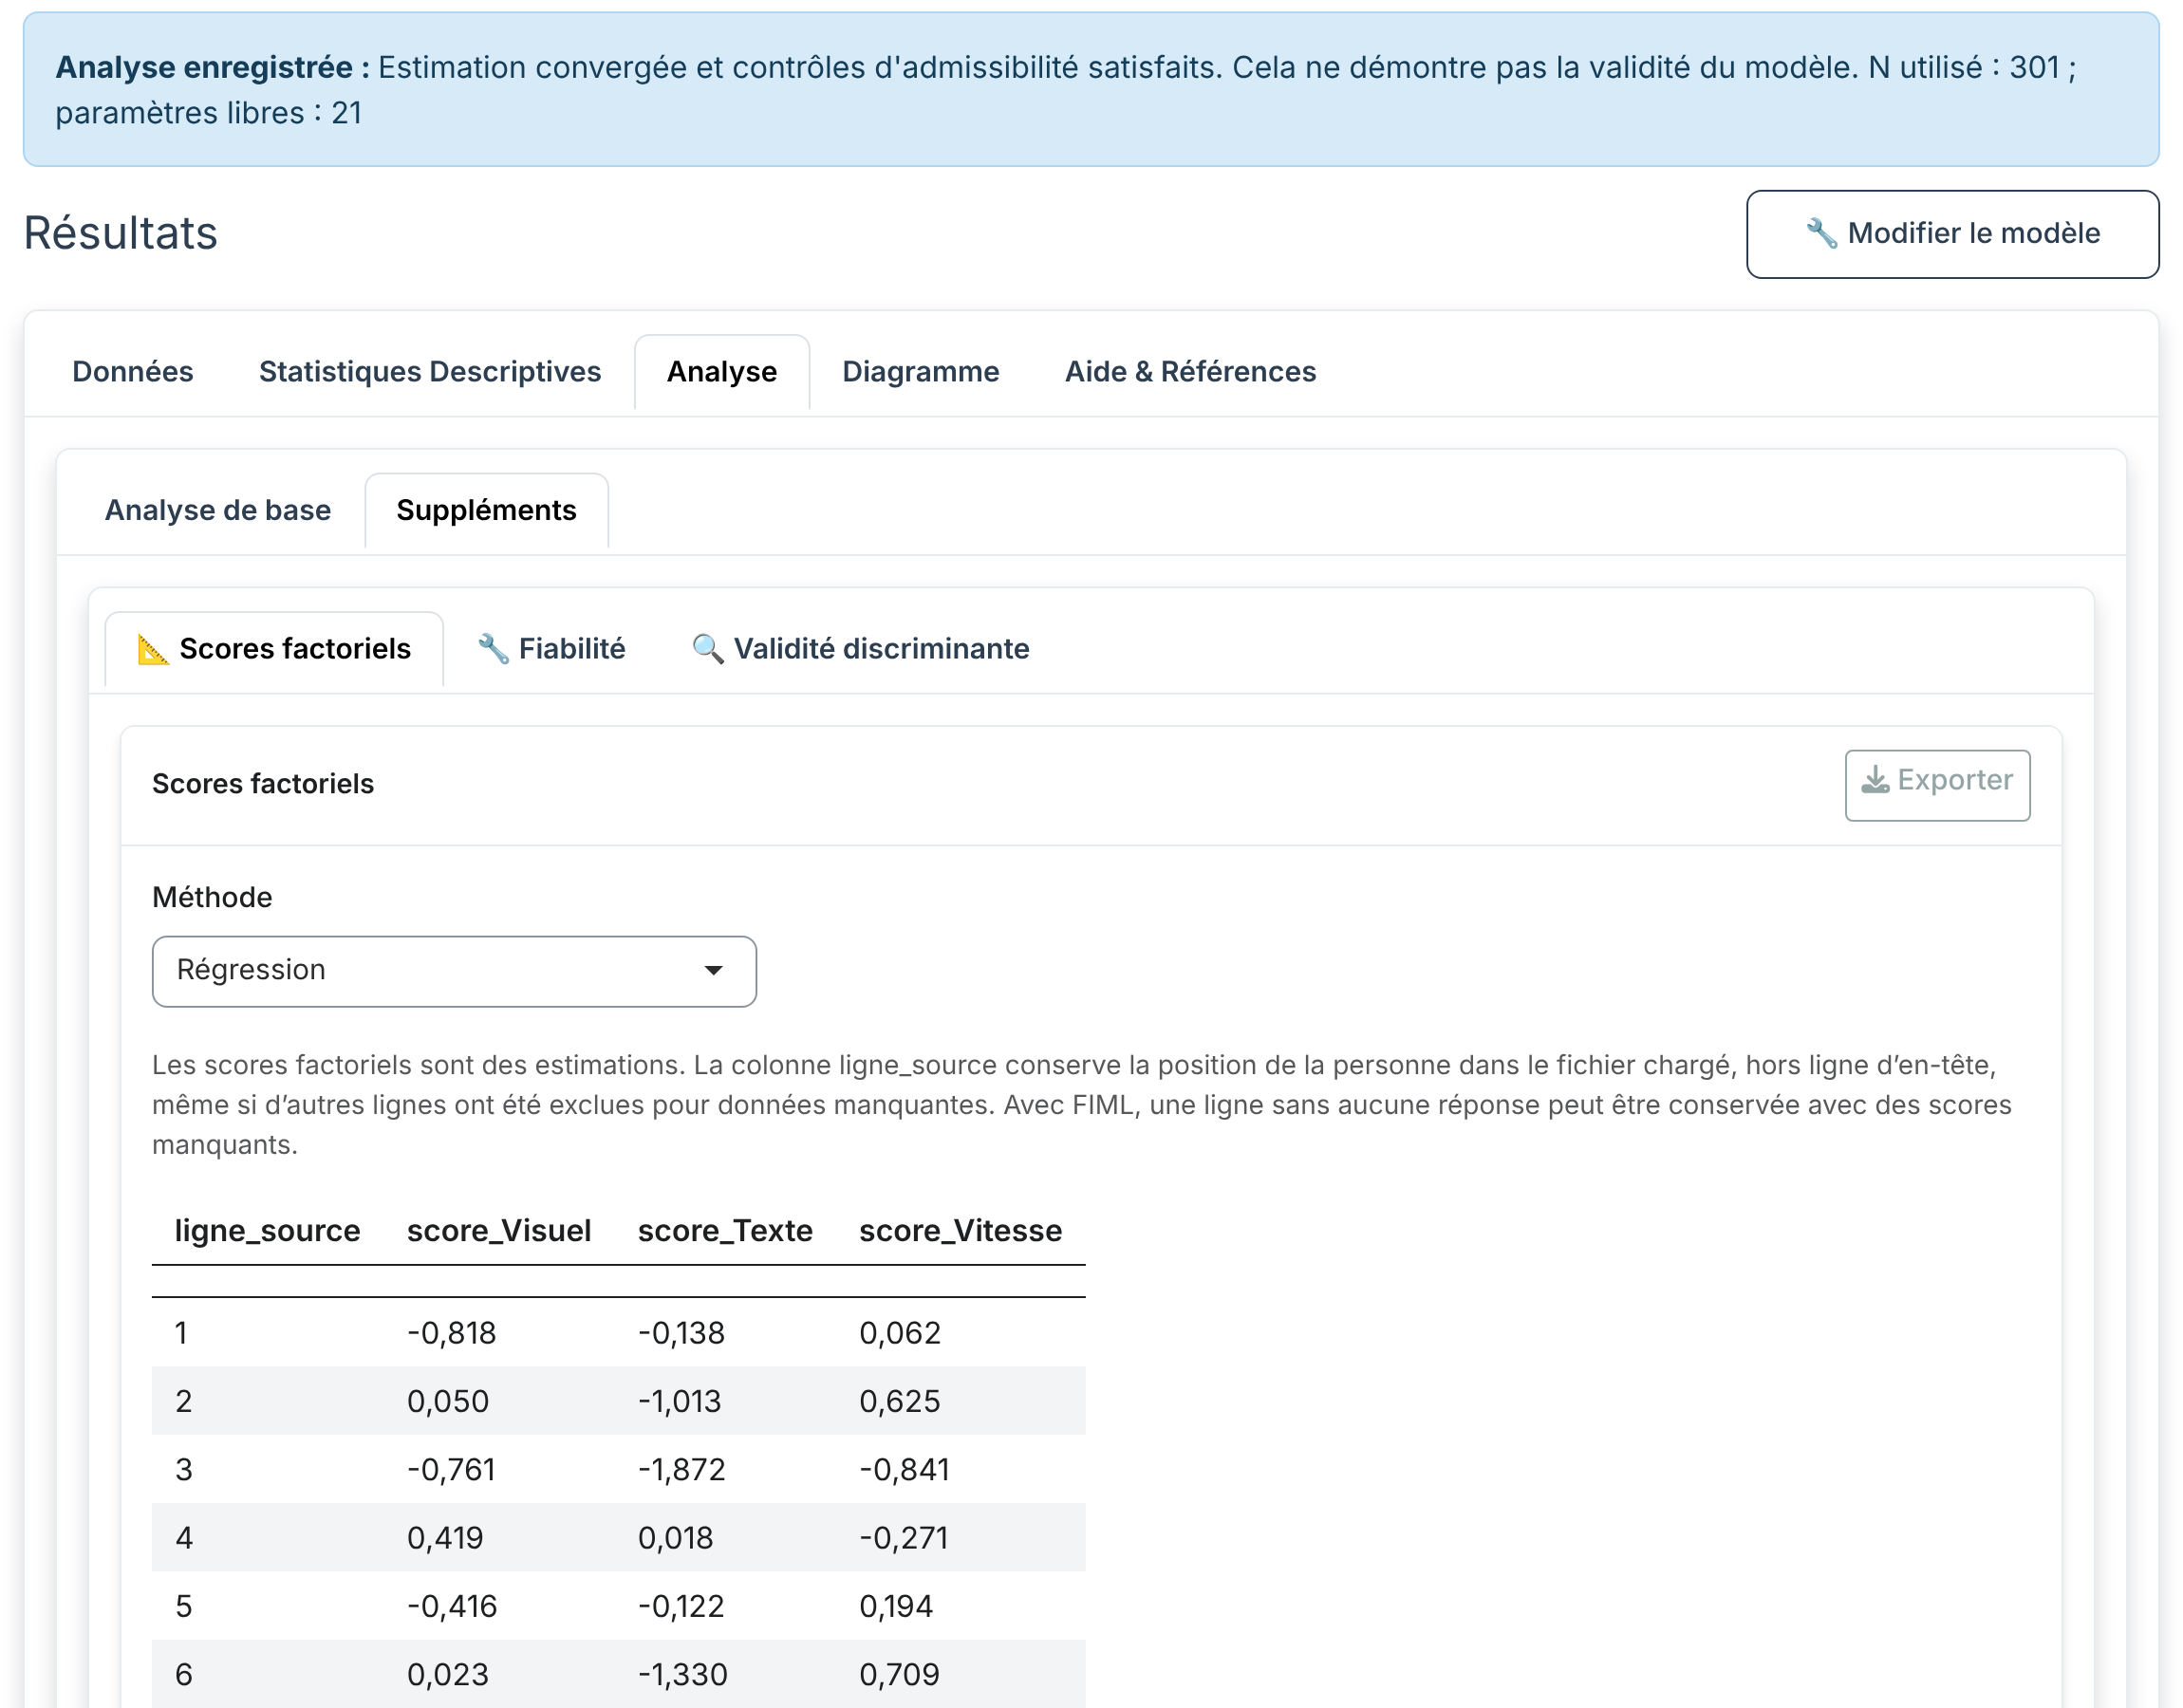
\includegraphics[width=1\linewidth,height=\textheight,keepaspectratio]{images/app/ch12_scores.png}

}

\caption{\label{fig-app-scores}\textbf{Suppléments → Scores factoriels}
: méthode, bouton \textbf{Exporter} et tableau des scores avec la
colonne \texttt{ligne\_source}.}

\end{figure}%

Ces scores dépendent des paramètres du modèle, de la convention
d'échelle et de la méthode choisie. Deux méthodes peuvent produire des
scores différents sans qu'une erreur de saisie se soit produite. Les
scores factoriels ne sont pas des valeurs observées sans incertitude.
Leur utilisation comme variables ordinaires dans une analyse ultérieure
demande donc une réflexion sur l'erreur d'estimation qu'elle laisse de
côté.

Une valeur positive ne signifie pas nécessairement « élevée » dans un
sens universel. Le sens et l'échelle dépendent de l'orientation des
facteurs et du modèle. Vérifiez les saturations et le codage avant
d'attribuer une étiquette substantielle à un score.

\section{Exporter sans perdre la correspondance des
personnes}\label{exporter-sans-perdre-la-correspondance-des-personnes}

Cliquez sur \textbf{Exporter} dans le panneau des scores. Le fichier
contient une colonne \textbf{\texttt{ligne\_source}} et des colonnes
comme \texttt{score\_Visuel}, \texttt{score\_Texte} et
\texttt{score\_Vitesse}. \texttt{ligne\_source} donne la position de la
personne dans le fichier chargé, hors en-tête.

\Needspace{9\baselineskip}

{

\begin{longtable}[]{@{}rrrr@{}}

\caption{\label{tbl-scores}Premières lignes de l'export des scores
(méthode Régression, modèle HS de référence).}

\tabularnewline

\toprule\noalign{}
ligne\_source & score\_Visuel & score\_Texte & score\_Vitesse \\
\midrule\noalign{}
\endhead
\bottomrule\noalign{}
\endlastfoot
1 & −0,818 & −0,138 & 0,062 \\
2 & 0,050 & −1,013 & 0,625 \\
3 & −0,761 & −1,872 & −0,841 \\
4 & 0,419 & 0,018 & −0,271 \\
5 & −0,416 & −0,122 & 0,194 \\

\end{longtable}

}

Lorsque des cas ont été exclus, il ne faut pas coller la première ligne
de score sur la première personne restante d'un fichier que l'on aurait
réorganisé autrement. Utilisez cette colonne pour l'appariement et
conservez aussi un identifiant d'origine dans votre dossier de données
lorsque vous en disposez.

Avec FIML, certaines lignes peuvent avoir des scores manquants,
notamment si aucune réponse utilisable ne permet une prédiction.
L'application ne doit pas inventer un score pour remplir le fichier. Si
une méthode de score n'est pas compatible avec l'analyse, lisez le
message et revenez à une méthode appropriée; ne changez pas la nature
des variables pour obtenir un export.

\section{Lire le nuage de scores}\label{lire-le-nuage-de-scores}

Pour plusieurs facteurs, le panneau de dispersion permet de comparer
deux ensembles de scores. La relation observée entre ces estimations
individuelles n'est pas nécessairement identique à la corrélation entre
facteurs du modèle. Elle dépend aussi de la méthode de prédiction et de
l'incertitude de mesure.

\Needspace{7\baselineskip}

{

\begin{longtable}[]{@{}lrr@{}}

\caption{\label{tbl-scores-cor}Corrélations entre scores factoriels
exportés (Régression) et corrélations entre facteurs du modèle.}

\tabularnewline

\toprule\noalign{}
Paire & Entre scores & Entre facteurs \\
\midrule\noalign{}
\endhead
\bottomrule\noalign{}
\endlastfoot
Visuel -- Texte & 0,552 & 0,459 \\
Visuel -- Vitesse & 0,593 & 0,471 \\
Texte -- Vitesse & 0,346 & 0,283 \\

\end{longtable}

}

Sur HS, les deux colonnes ne coïncident pas. Les scores de régression «
tirent » chaque personne vers la moyenne en proportion de l'incertitude
de sa mesure, et un score dépend aussi des indicateurs des autres
facteurs. Les corrélations entre scores ne sont donc pas un substitut
aux corrélations entre facteurs estimées par le modèle.

Une forme inhabituelle du nuage peut inviter à examiner les observations
ou les prédictions. Elle ne constitue pas à elle seule la preuve d'une
sous-population ou d'un mécanisme causal.

\section{Préparer un diagramme
utile}\label{pruxe9parer-un-diagramme-utile}

Dans \textbf{Diagramme}, commencez par une disposition lisible, des noms
complets et des coefficients standardisés lorsque votre objectif est de
comparer la force des relations. Les options de forme, de couleur et de
taille changent la représentation, pas les paramètres estimés.

\begin{figure}[htbp]

\centering{

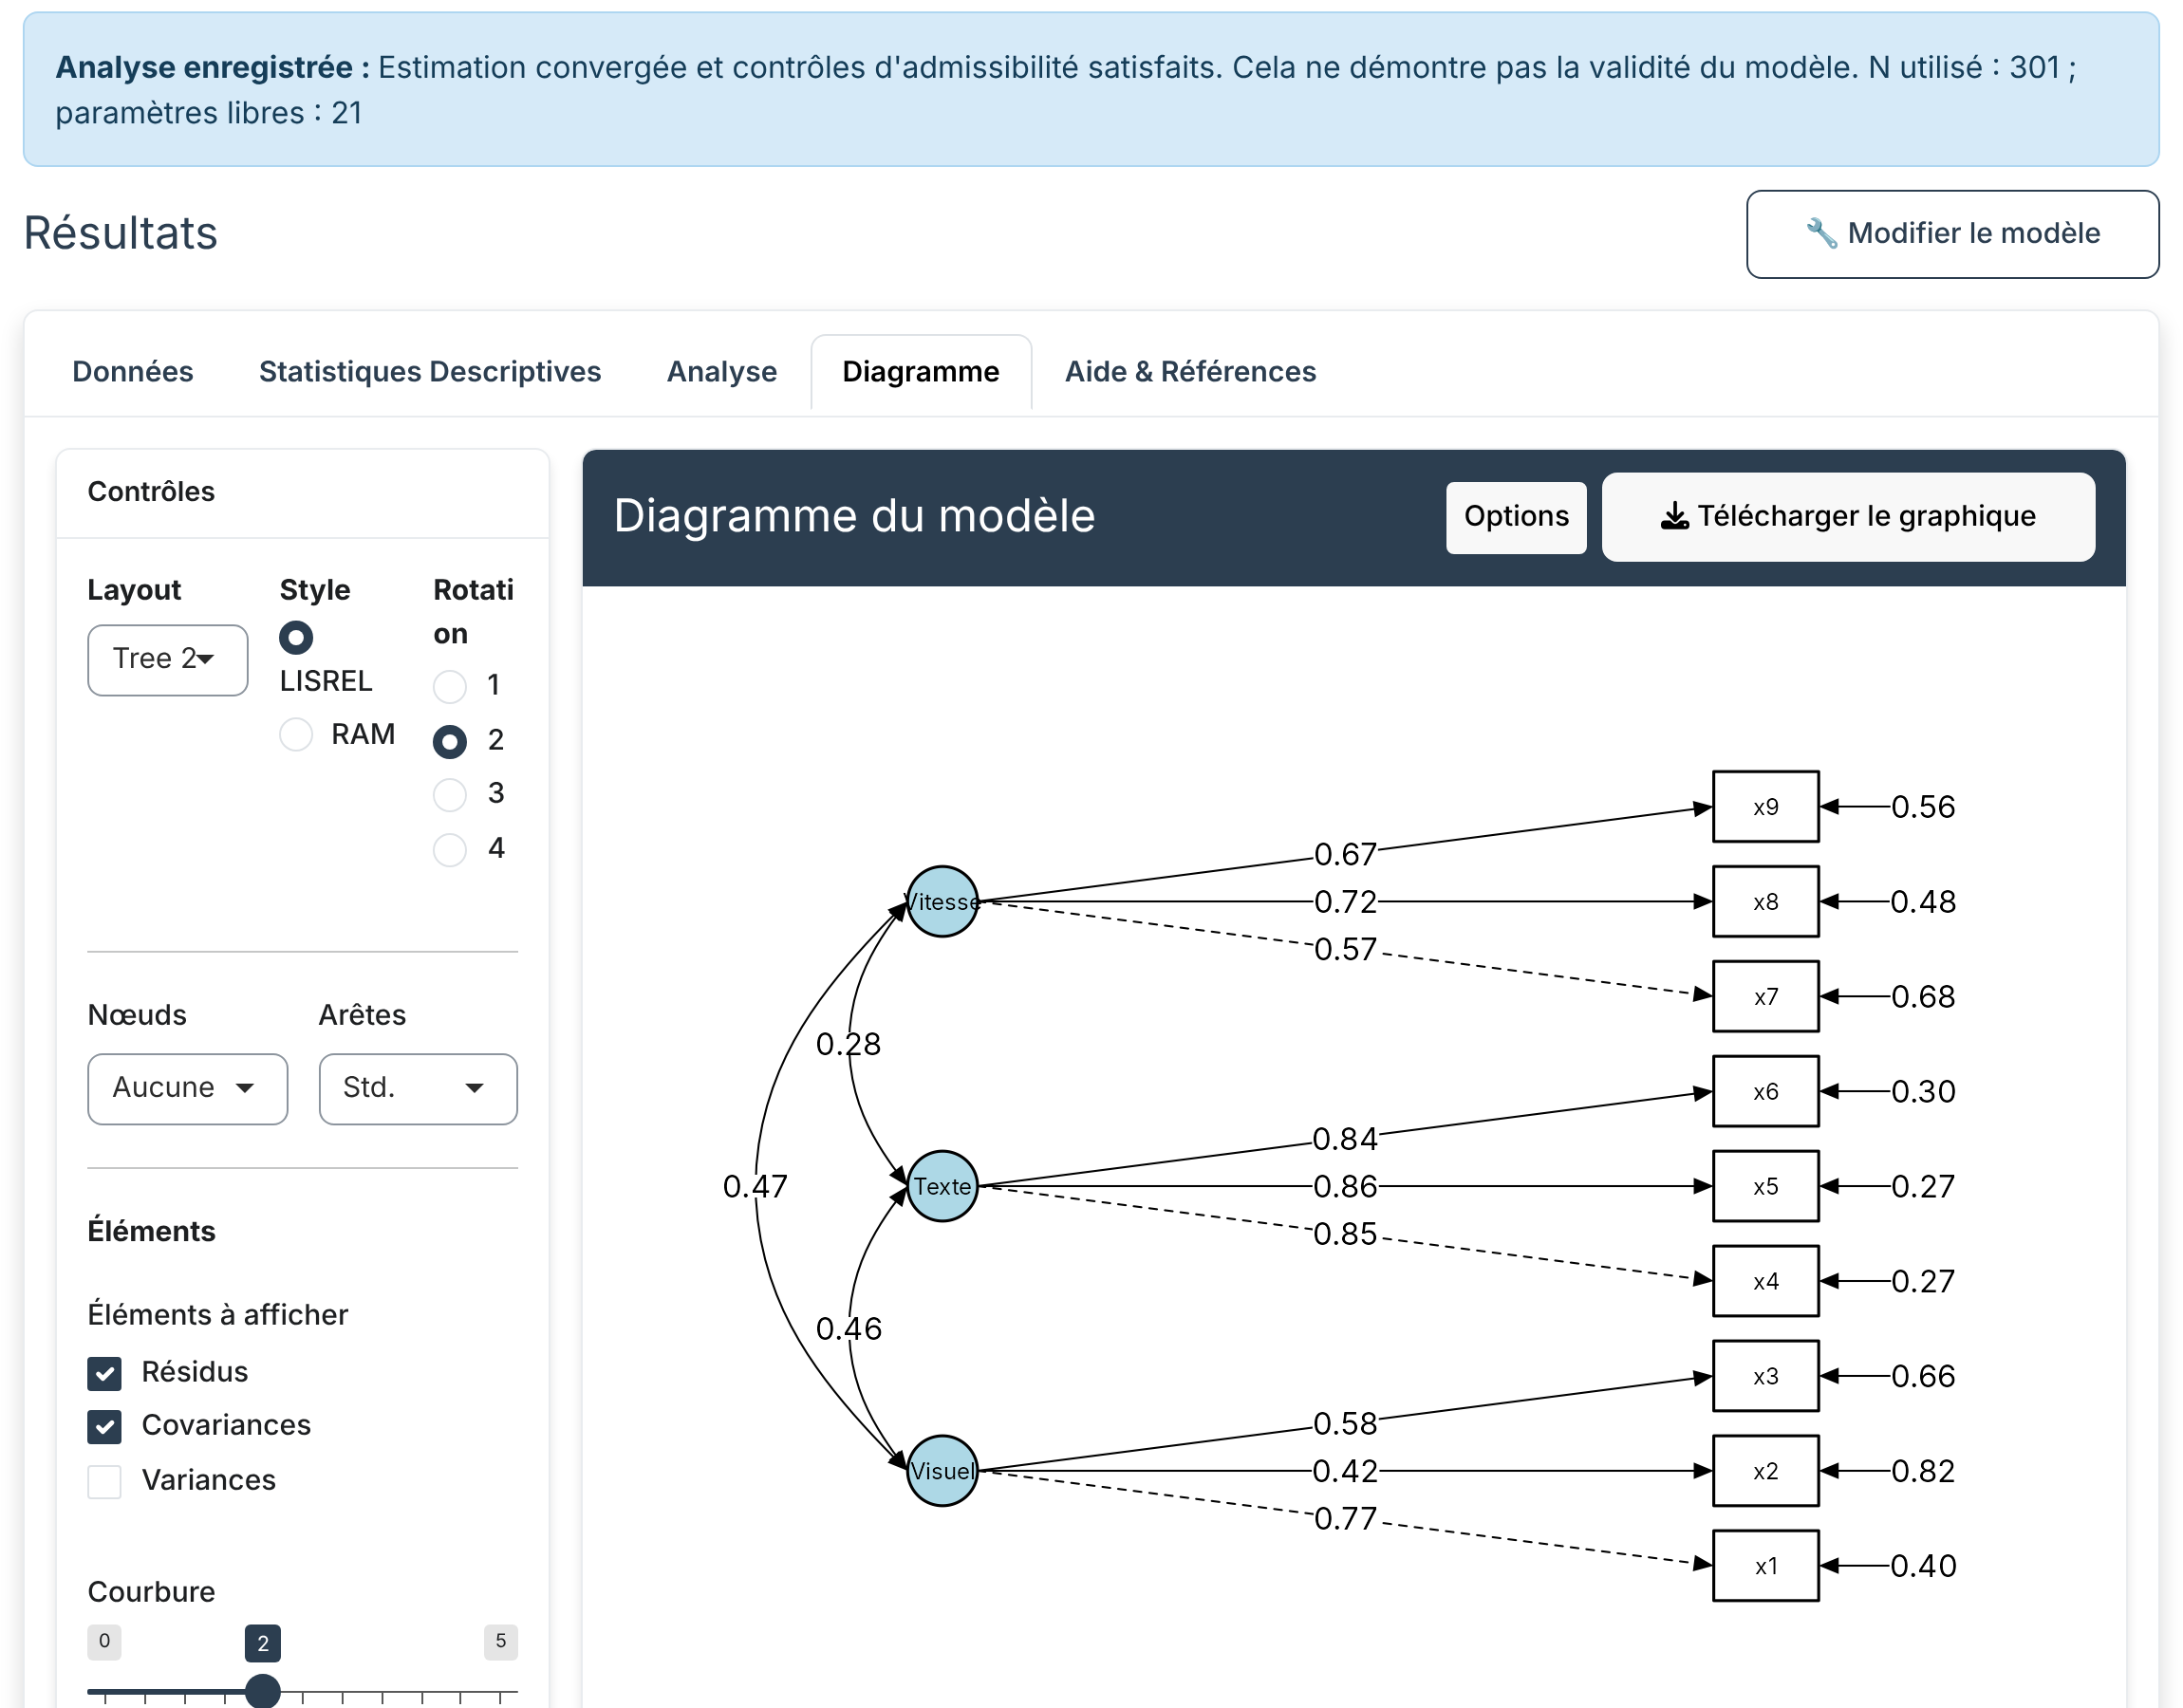
\includegraphics[width=1\linewidth,height=\textheight,keepaspectratio]{images/app/ch12_diagramme.png}

}

\caption{\label{fig-app-diagramme}\textbf{Diagramme} : le modèle estimé
avec ses coefficients standardisés. Les contrôles de gauche règlent la
disposition, le style, les éléments affichés et la courbure;
\textbf{Télécharger le graphique} exporte l'image.}

\end{figure}%

Précisez dans la légende si les nombres sont standardisés ou non. Une
flèche à double sens entre facteurs représente une association; elle ne
désigne pas automatiquement une influence causale réciproque. Les
résidus doivent rester identifiables si leur rôle est discuté.

Le diagramme conceptuel de la configuration décrit la structure avant
estimation. Le diagramme des résultats représente l'analyse enregistrée.
Cette différence doit rester explicite lorsque vous incorporez une
figure à un travail.

\section{Télécharger le rapport}\label{tuxe9luxe9charger-le-rapport}

Dans \textbf{Analyse → Analyse de base}, \textbf{Télécharger le rapport}
génère un document HTML de l'analyse estimée. Il reprend notamment les
informations de méthode, les paramètres, les indices, les avertissements
et les compléments effectivement calculés. Il ne remplace pas la
rédaction d'une interprétation argumentée.

Si vous avez demandé les intervalles HTMT compatibles, vérifiez qu'ils
figurent dans le rapport téléchargé. Enregistrez un document distinct
pour chaque modèle important. Un nom tel que
\texttt{MSQ\_WLSMV\_2facteurs.html} est plus informatif que plusieurs
fichiers appelés simplement \texttt{rapport.html}.

Les changements non estimés portant sur le modèle, les données ou la
méthode ne remplacent pas l'analyse enregistrée dont provient le
rapport. Le bandeau de configuration modifiée rappelle cette
distinction. Les options de présentation peuvent changer les éléments
affichés. Pour produire un rapport d'un nouveau modèle, estimez-le
d'abord.

\section{Une trame de rédaction}\label{une-trame-de-ruxe9daction}

Une présentation reproductible peut tenir en six paragraphes, dont la
longueur dépend de l'enjeu :

\begin{enumerate}
\def\labelenumi{\arabic{enumi}.}
\tightlist
\item
  \textbf{Question et contexte.} Décrire les construits, l'échantillon
  et la justification du modèle.
\item
  \textbf{Variables.} Nommer les indicateurs, leurs catégories ou unités
  et les recodages réellement effectués.
\item
  \textbf{Méthode.} Préciser l'estimateur, l'identification, les
  absences et l'effectif utilisé.
\item
  \textbf{Résultats.} Présenter les paramètres substantiels, les indices
  avec leurs versions et les diagnostics importants.
\item
  \textbf{Qualité de mesure.} Discuter la fiabilité, la distinction des
  facteurs et les limites des indices.
\item
  \textbf{Conclusion.} Répondre à la question et indiquer ce qui reste
  incertain ou demanderait une autre étude.
\end{enumerate}

Ne remplacez pas ces paragraphes par un empilement de tableaux. Un
lecteur doit pouvoir comprendre pourquoi le modèle a été estimé et ce
qui découle des résultats.

\section{Le code reste facultatif}\label{le-code-reste-facultatif}

Le mode avancé donne accès, dans l'onglet \textbf{Code}, au code R
exportable et à une ébauche Stata. Le script R contient les données
analysées, le modèle et les options de l'estimation affichée : il
reproduit exactement l'analyse dans R. Ces éléments peuvent servir à un
audit ou à une reprise de l'analyse par une personne compétente. Ils ne
sont pas nécessaires pour réaliser les activités du manuel. L'ébauche
Stata ne garantit pas une équivalence de calcul avec le moteur utilisé
dans l'application.

\begin{figure}[htbp]

\centering{

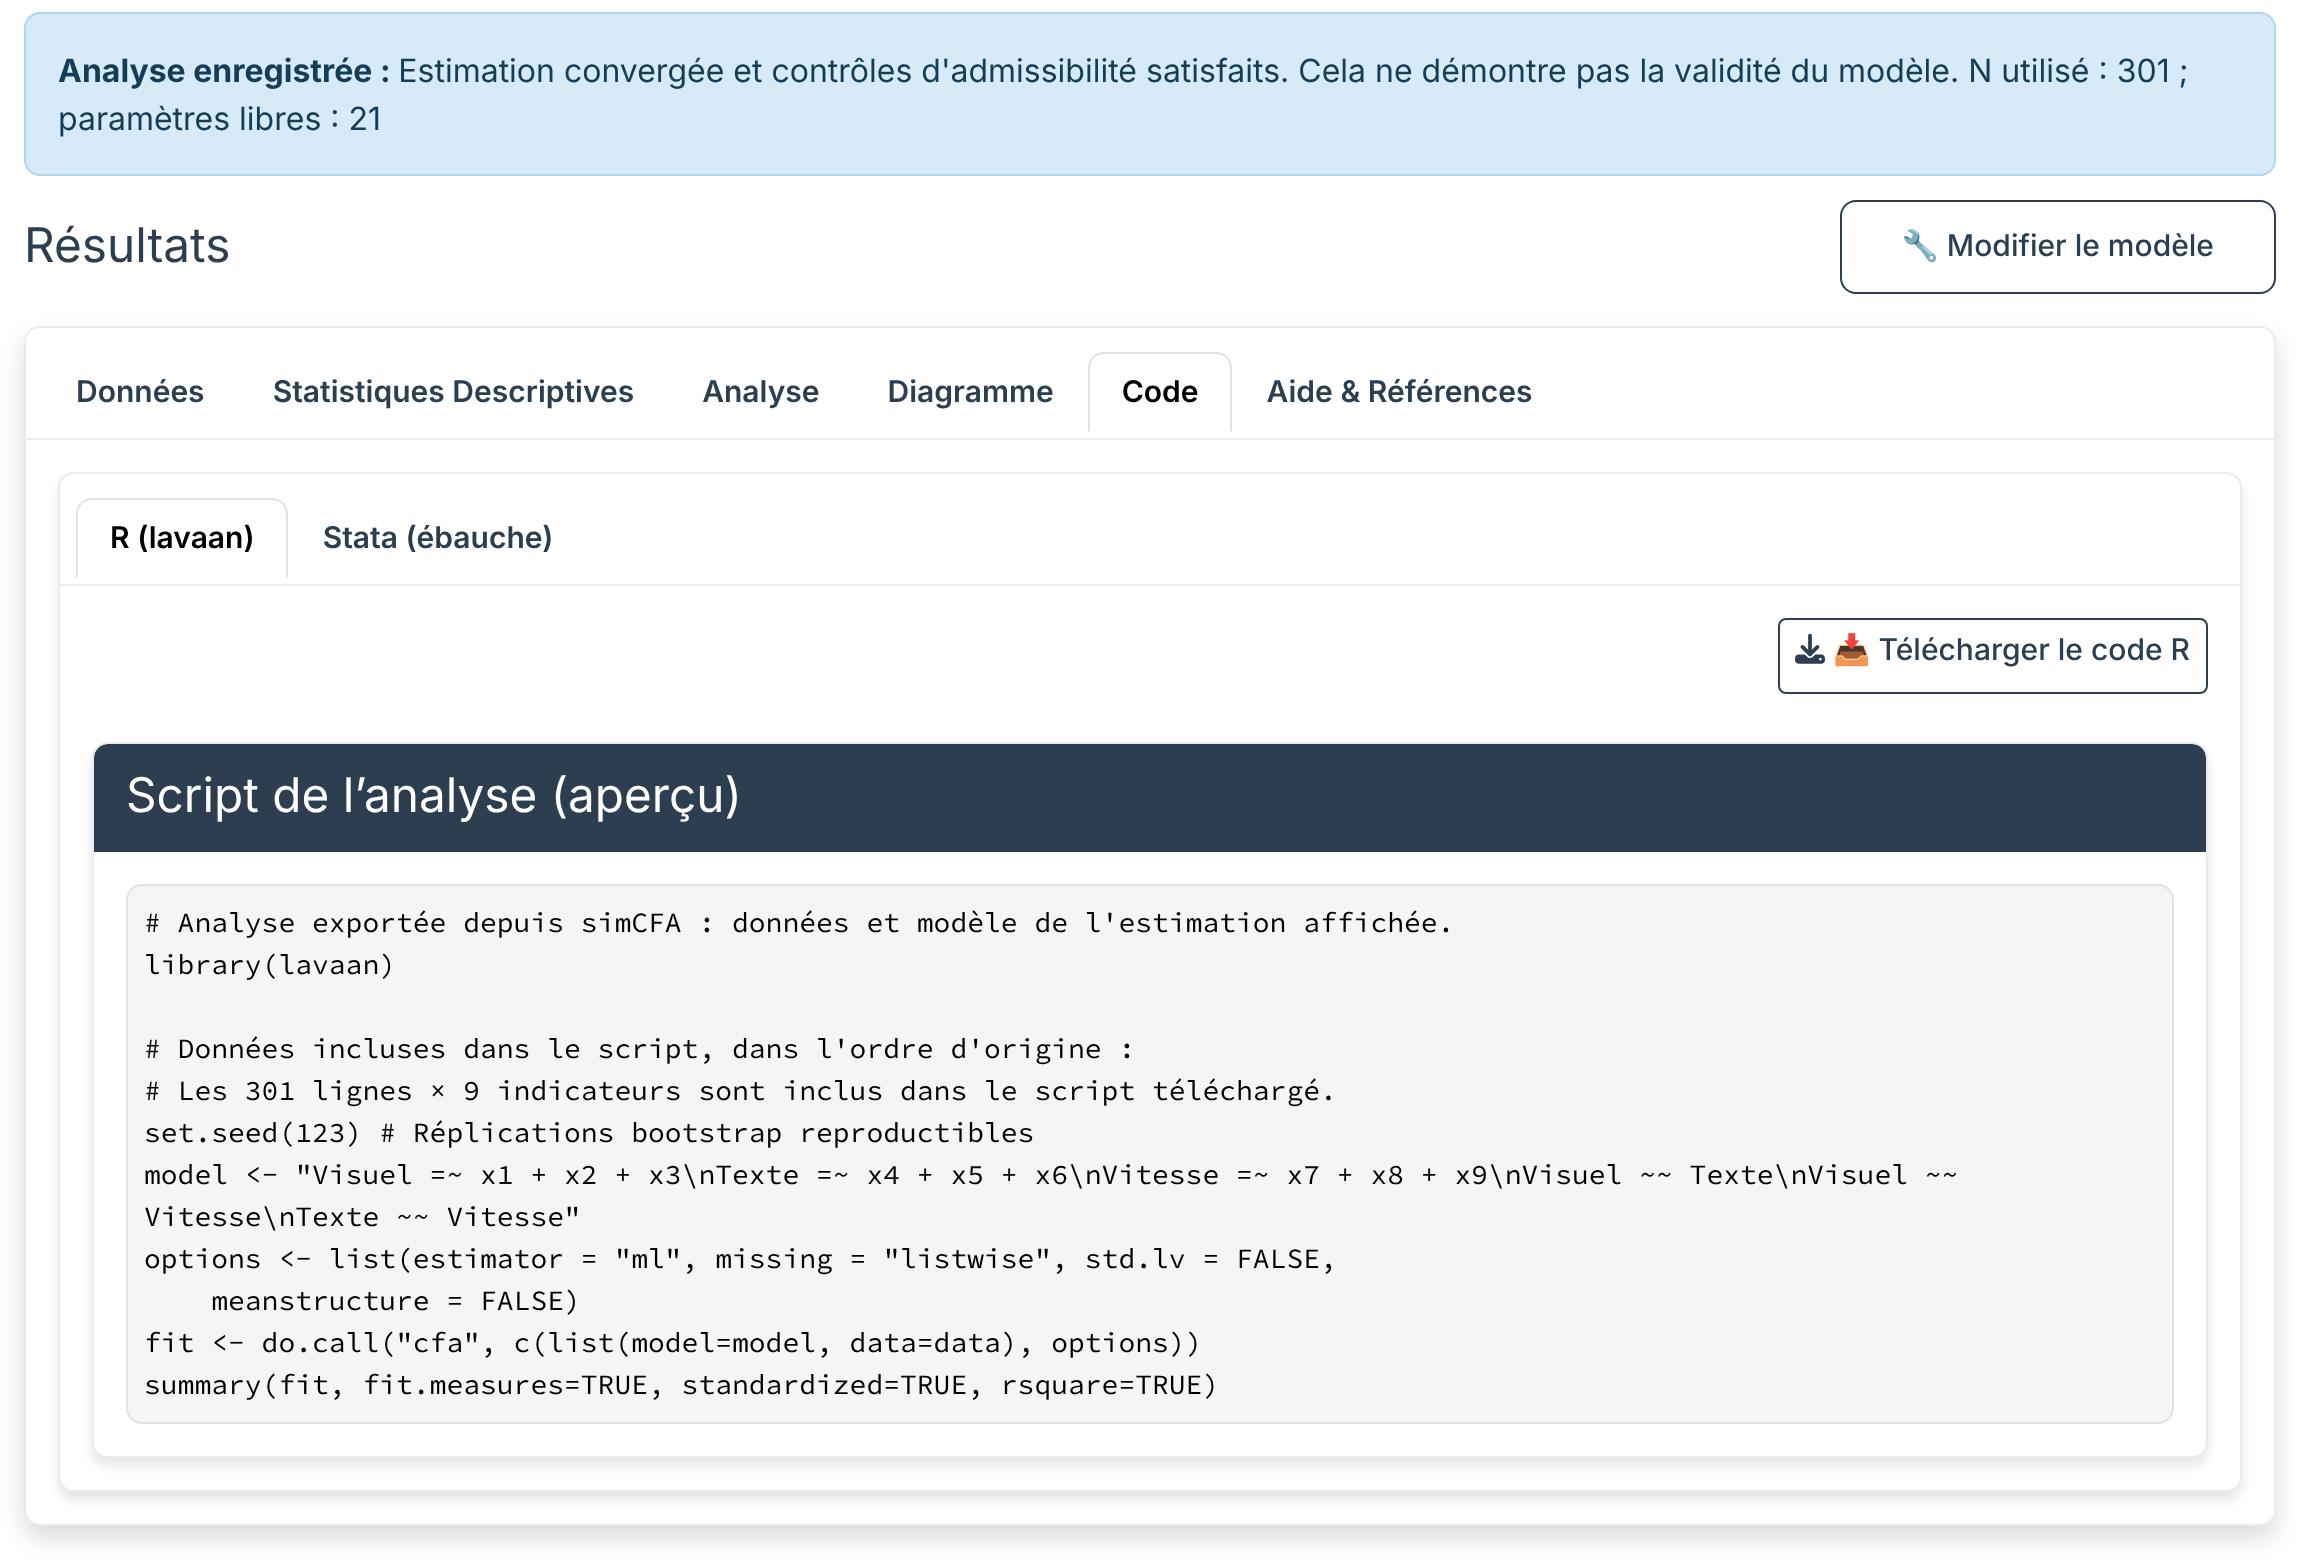
\includegraphics[width=1\linewidth,height=\textheight,keepaspectratio]{images/app/ch12_code.png}

}

\caption{\label{fig-app-code}\textbf{Code → R (lavaan)} en
\textbf{Options avancées} : le script reproduit l'analyse enregistrée,
données comprises.}

\end{figure}%

\section{Laboratoire : une page
autonome}\label{laboratoire-une-page-autonome}

À partir de votre rapport HS, rédigez une page autonome comprenant une
petite figure et un tableau de paramètres choisis. Une personne qui ne
voit pas votre session doit pouvoir identifier les données, le modèle,
l'estimateur et les limites de votre conclusion. Vérifiez que chaque
nombre cité correspond au même modèle enregistré.

\begin{tcolorbox}[enhanced jigsaw, arc=.35mm, bottomrule=.15mm, bottomtitle=1mm, breakable, colback=white, colbacktitle=quarto-callout-tip-color!10!white, colframe=quarto-callout-tip-color-frame, coltitle=black, left=2mm, leftrule=.75mm, opacityback=0, opacitybacktitle=0.6, rightrule=.15mm, title={Réponse}, titlerule=0mm, toprule=.15mm, toptitle=1mm]

Une page satisfaisante contient au minimum : le nom du fichier et
l'effectif utilisé (301 élèves); la structure (trois facteurs corrélés,
trois tests chacun, aucune covariance résiduelle); la méthode (ML, λ₁=1,
cas complets); les indices avec leur version (χ² = 85,306, 24 dl; CFI
0,931; RMSEA 0,092 {[}0,071; 0,114{]}; SRMR 0,065, versions standard);
le diagramme avec une légende qui précise « coefficients standardisés »;
une phrase sur la fiabilité modeste du facteur visuel; une conclusion
qui mentionne les écarts d'ajustement. Le contrôle final consiste à
vérifier que tous ces nombres viennent du même rapport.

\end{tcolorbox}

\begin{tcolorbox}[enhanced jigsaw, arc=.35mm, bottomrule=.15mm, bottomtitle=1mm, breakable, colback=white, colbacktitle=quarto-callout-important-color!10!white, colframe=quarto-callout-important-color-frame, coltitle=black, left=2mm, leftrule=.75mm, opacityback=0, opacitybacktitle=0.6, rightrule=.15mm, title={À retenir}, titlerule=0mm, toprule=.15mm, toptitle=1mm]

\begin{itemize}
\tightlist
\item
  Un score factoriel est une prédiction qui dépend du modèle et de la
  méthode.
\item
  \texttt{ligne\_source} garantit l'appariement des scores aux personnes
  du fichier.
\item
  Les corrélations entre scores ne remplacent pas les corrélations entre
  facteurs.
\item
  Un rapport décrit l'analyse enregistrée : estimez avant de
  télécharger.
\end{itemize}

\end{tcolorbox}

\section{Quiz}\label{quiz-11}

\begin{enumerate}
\def\labelenumi{\arabic{enumi}.}
\tightlist
\item
  Pourquoi ne pas coller les scores exportés à côté du fichier d'origine
  sans regarder \texttt{ligne\_source} ?
\item
  Les scores Régression et Bartlett diffèrent. Lequel est le « vrai »
  score ?
\item
  Une flèche à double sens relie deux facteurs dans le diagramme. Que
  représente-t-elle ?
\item
  Le script R de l'onglet \textbf{Code} est-il nécessaire pour réaliser
  les activités ?
\end{enumerate}

\begin{tcolorbox}[enhanced jigsaw, arc=.35mm, bottomrule=.15mm, bottomtitle=1mm, breakable, colback=white, colbacktitle=quarto-callout-tip-color!10!white, colframe=quarto-callout-tip-color-frame, coltitle=black, left=2mm, leftrule=.75mm, opacityback=0, opacitybacktitle=0.6, rightrule=.15mm, title={Réponses}, titlerule=0mm, toprule=.15mm, toptitle=1mm]

\begin{enumerate}
\def\labelenumi{\arabic{enumi}.}
\tightlist
\item
  Si des cas ont été exclus, les lignes ne se correspondent plus une à
  une; \texttt{ligne\_source} donne la position exacte de chaque
  personne.
\item
  Aucun : ce sont deux méthodes de prédiction aux propriétés
  différentes.
\item
  Une covariance (ou corrélation) entre facteurs, sans direction
  causale.
\item
  Non. Il sert à l'audit ou à la reprise de l'analyse dans R.
\end{enumerate}

\end{tcolorbox}

\bookmarksetup{startatroot}

\chapter{Ateliers guidés sur les données réelles}\label{sec-ateliers}

\begin{tcolorbox}[enhanced jigsaw, arc=.35mm, bottomrule=.15mm, bottomtitle=1mm, breakable, colback=white, colbacktitle=quarto-callout-note-color!10!white, colframe=quarto-callout-note-color-frame, coltitle=black, left=2mm, leftrule=.75mm, opacityback=0, opacitybacktitle=0.6, rightrule=.15mm, title={Comment utiliser ces ateliers}, titlerule=0mm, toprule=.15mm, toptitle=1mm]

Sept ateliers, un par jeu de données, reprennent les notions des
chapitres précédents dans une situation complète. Chacun précise les
données, la question, les réglages, les étapes, les questions et la
production attendue. Les corrigés sont réunis dans l'annexe des corrigés
: rédigez d'abord vos réponses.

\end{tcolorbox}

Chaque atelier peut être repris indépendamment. Commencez par
\textbf{Données réelles}, sélectionnez le fichier indiqué et cliquez sur
\textbf{Charger cet exemple et son modèle}. Ce point de départ évite de
conserver d'anciennes associations ou contraintes. Les corrigés sont
réunis dans l'annexe correspondante; prenez d'abord vos propres notes.

Les productions demandées sont des rapports HTML et de courts
commentaires. Vous n'avez pas à produire de syntaxe R ou à accéder au
projet source du manuel.

\section{Atelier A sur les aptitudes
cognitives}\label{atelier-a-sur-les-aptitudes-cognitives}

\textbf{Données.} Holzinger--Swineford, 301 élèves, neuf indicateurs.
\textbf{Question.} La structure à trois aptitudes paraît-elle
défendable, et avec quelles limites ? \textbf{Réglages.} Trois facteurs
préparés, ML, λ₁=1, cas complets, aucun item ordinal, aucune covariance
résiduelle ajoutée.

\begin{enumerate}
\def\labelenumi{\arabic{enumi}.}
\tightlist
\item
  Vérifiez les groupes \texttt{x1}--\texttt{x3},
  \texttt{x4}--\texttt{x6}, \texttt{x7}--\texttt{x9}, puis estimez.
\item
  Relevez l'effectif, les degrés de liberté et les saturations
  entièrement standardisées.
\item
  Consultez l'ajustement, la fiabilité et les corrélations factorielles.
\item
  Téléchargez le rapport avant toute modification.
\end{enumerate}

\textbf{Questions.} A1. Quel indicateur visuel paraît le moins fortement
relié à son facteur ? A2. Quel facteur présente l'AVE la plus élevée ?
A3. Les paramètres et l'ajustement conduisent-ils exactement au même
jugement ? A4. Quelle conclusion provisoire tient compte des deux ?

\textbf{Production.} Un rapport et un commentaire de 200 à 300 mots,
sans suppression d'item fondée sur un seuil isolé.

\section{Atelier B sur la démocratie
politique}\label{atelier-b-sur-la-duxe9mocratie-politique}

\textbf{Données.} Démocratie politique de Bollen, 75 pays et onze
indicateurs. \textbf{Question.} Que signifie distinguer deux mesures de
démocratie à deux moments tout en les trouvant très fortement liées ?
\textbf{Réglages.} Les trois facteurs préparés, ML, λ₁=1, cas complets,
indicateurs traités comme continus.

Le modèle comprend \texttt{Democratie60} avec \texttt{y1} à \texttt{y4},
\texttt{Democratie65} avec \texttt{y5} à \texttt{y8} et
\texttt{Industrialisation} avec \texttt{x1} à \texttt{x3}. Il ne
contient ni les régressions du modèle structurel de Bollen ni une
analyse d'invariance longitudinale. Les mêmes types d'indicateurs sont
observés aux deux moments; une spécificité de mesure commune peut donc
demeurer.

\begin{enumerate}
\def\labelenumi{\arabic{enumi}.}
\tightlist
\item
  Chargez et estimez ce modèle sans modification.
\item
  Relevez la corrélation entre les deux facteurs de démocratie.
\item
  Comparez le CFI, le RMSEA et le SRMR.
\item
  Consultez le panneau de validité discriminante et examinez les limites
  de sa lecture.
\end{enumerate}

\textbf{Questions.} B1. L'effectif de 75 interdit-il automatiquement
toute estimation ? B2. Que suggère une corrélation factorielle proche de
1 ? B3. Pourquoi ne peut-on pas conclure ici à une influence causale de
l'industrialisation ? B4. Peut-on annoncer que le changement de
démocratie entre 1960 et 1965 a été mesuré de manière invariante ?

\textbf{Production.} Une page distinguant explicitement estimation,
précision, distinction des mesures et absence d'un modèle causal ou
d'invariance testé.

\section{Atelier C sur deux sections du
LSAT}\label{atelier-c-sur-deux-sections-du-lsat}

\textbf{Données.} LSAT 6 et LSAT 7, analysés séparément, 1\,000
observations et cinq items chacun. \textbf{Question.} Un modèle simple
peut-il donner des diagnostics différents sur deux séries de réponses
binaires ? \textbf{Réglages.} Un facteur \texttt{Aptitude}, Q1 à Q5,
cinq items ordinaux, WLSMV, cas complets.

\begin{enumerate}
\def\labelenumi{\arabic{enumi}.}
\tightlist
\item
  Estimez LSAT 6 et conservez son rapport.
\item
  Chargez ensuite LSAT 7 et son modèle préparé; estimez-le.
\item
  Vérifiez l'effectif et les cinq degrés de liberté dans chaque cas.
\item
  Relevez les indices avec leur version, puis comparez les deux
  ensembles descriptivement.
\end{enumerate}

\textbf{Questions.} C1. Pourquoi le tableau de normalité univariée
est-il remplacé par une note ? C2. Un CFI de 1 et un RMSEA de 0
démontrent-ils une mesure parfaite ? C3. Pourquoi ne faut-il pas
fusionner les fichiers ligne par ligne ? C4. Quelle différence de
version pourrait expliquer deux RMSEA différents pour LSAT 7 ?

\textbf{Production.} Deux rapports et un tableau de comparaison qui
nomme les versions Standard, Scaled ou Robust. Aucun test de différence
entre ces deux échantillons distincts n'est demandé.

\section{Atelier D sur les seize items cognitifs
SAPA}\label{atelier-d-sur-les-seize-items-cognitifs-sapa}

\textbf{Données.} SAPA / ability, 1\,525 personnes et seize réponses
binaires. \textbf{Question.} Quelle organisation de premier ordre décrit
les quatre familles de tâches ? \textbf{Réglages.} Quatre facteurs
préparés, seize items ordinaux, WLSMV, cas complets.

Les groupes sont \texttt{reason.*} pour le raisonnement,
\texttt{letter.*} pour les séries de lettres, \texttt{matrix.*} pour les
matrices et \texttt{rotate.*} pour les rotations. Les astérisques
utilisés ici signifient « les variables de ce groupe », pas un caractère
à saisir : le modèle préparé sélectionne les noms exacts.

\begin{enumerate}
\def\labelenumi{\arabic{enumi}.}
\tightlist
\item
  Vérifiez quatre items dans chacun des quatre facteurs.
\item
  Estimez et relevez les 1\,248 cas complets.
\item
  Comparez les saturations et les corrélations entre facteurs.
\item
  Ouvrez la carte des corrélations, puis comparez l'ordre des facteurs
  et l'ordre empirique.
\end{enumerate}

\textbf{Questions.} D1. Pourquoi l'effectif estimé diffère-t-il de
l'effectif chargé ? D2. Des facteurs corrélés constituent-ils déjà un
facteur général de second ordre ? D3. Le regroupement empirique de la
carte suffit-il à valider les quatre dimensions ? D4. Quelle information
supplémentaire faudrait-il pour discuter une réponse atypique à un item
de matrices ?

\textbf{Production.} Un rapport et un schéma conceptuel des quatre
dimensions, sans ajouter de facteur général non estimé. La notice de la
source souligne certaines particularités des items de matrices :
utilisez-la pour nuancer votre commentaire.

\section{Atelier E sur les états affectifs
MSQ}\label{atelier-e-sur-les-uxe9tats-affectifs-msq}

\textbf{Données.} MSQ, vingt adjectifs, première occasion de mesure pour
3\,032 participants. \textbf{Question.} Peut-on obtenir une forte
fiabilité et un modèle globalement mal ajusté ? \textbf{Réglages.} Deux
facteurs préparés, dix indicateurs chacun, vingt items ordinaux, WLSMV,
cas complets.

\begin{enumerate}
\def\labelenumi{\arabic{enumi}.}
\tightlist
\item
  Vérifiez les vingt indicateurs et estimez sur les 2\,951 cas complets.
\item
  Consultez \textbf{4. Interpréter} et notez les versions du CFI et du
  RMSEA.
\item
  Comparez ces résultats aux colonnes de la sortie détaillée.
\item
  Relevez oméga et AVE, puis examinez les signaux sans modifier le
  modèle.
\end{enumerate}

\textbf{Questions.} E1. Pourquoi n'utilise-t-on pas les 6 411 lignes du
fichier MSQ complet de la source ? E2. Un oméga élevé résout-il les
difficultés d'ajustement ? E3. Quelle cible décrit cet oméga ordinal ?
E4. Quelles justifications seraient nécessaires avant d'ajouter des
liens résiduels entre adjectifs proches ?

\textbf{Production.} Une conclusion argumentée distinguant distribution
ordinale, répétitions de mesure, fiabilité et ajustement. L'étude
complète suivante approfondit cet exemple.

\section{Atelier F sur la personnalité et les items
inversés}\label{atelier-f-sur-la-personnalituxe9-et-les-items-inversuxe9s}

\textbf{Données.} BFI / SAPA, 2\,800 personnes et vingt-cinq items.
\textbf{Question.} Pourquoi certains coefficients de fiabilité de la
somme brute peuvent-ils être très faibles malgré des liens factoriels
substantiels ? \textbf{Réglages.} Cinq facteurs préparés, cinq items
chacun, déclarations ordinales, WLSMV, cas complets, aucun recodage.

\begin{enumerate}
\def\labelenumi{\arabic{enumi}.}
\tightlist
\item
  Estimez le modèle préparé et vérifiez les 2\,436 cas complets.
\item
  Examinez les signes des saturations par groupe.
\item
  Consultez les indices de fiabilité et relisez les clés des items
  orientés en sens inverse.
\item
  Comparez la cible de la somme brute à celle de H et à celle d'une
  somme qui serait recodée.
\end{enumerate}

\textbf{Questions.} F1. Une saturation négative constitue-t-elle
toujours une erreur ? F2. Pourquoi une valeur négative d'alpha ne
doit-elle pas être transformée arbitrairement en zéro ou en valeur
absolue ? F3. Quel serait le recodage d'un item inversé de 1 à 6 ? F4.
Peut-on déclarer la somme brute fiable en citant seulement H ?

\textbf{Production.} Une note expliquant le rôle du codage. Aucun
recodage n'est demandé dans l'application : l'activité porte précisément
sur le fichier original. Ces données IPIP/SAPA ne sont pas le Big Five
Inventory d'Oliver John, malgré le nom abrégé du fichier.

\section{Atelier G sur les réponses
partielles}\label{atelier-g-sur-les-ruxe9ponses-partielles}

\textbf{Données.} \texttt{HS\_absences\_pedagogiques.csv}, dont la
provenance et l'accès sont détaillés dans le chapitre sur les absences.
\textbf{Question.} Que conserve-t-on et que suppose-t-on avec FIML ?
\textbf{Réglages.} Modèle HS à trois facteurs, indicateurs continus, ML,
puis comparaison des cas complets et de FIML.

\begin{enumerate}
\def\labelenumi{\arabic{enumi}.}
\tightlist
\item
  Importez le fichier dérivé et vérifiez ses en-têtes.
\item
  Reconstituez les trois groupes HS avec leurs noms.
\item
  Estimez par cas complets et conservez le rapport.
\item
  Changez uniquement la gestion des absences pour FIML, estimez et
  conservez un second rapport.
\item
  Exportez les scores et repérez \texttt{ligne\_source}.
\end{enumerate}

\textbf{Questions.} G1. Pourquoi obtient-on 211 cas complets ? G2.
Pourquoi FIML peut-il conserver les 301 personnes de ce fichier ? G3.
Pourquoi les tests multivariés de normalité et alpha peuvent-ils
afficher d'autres effectifs ? G4. Une meilleure valeur d'un indice
prouve-t-elle que les absences seraient MAR ?

\textbf{Production.} Deux rapports, une note de méthode et une
explication de l'appariement des scores au fichier d'origine.

\bookmarksetup{startatroot}

\chapter{Construire une conclusion autonome sur un
modèle}\label{sec-etude}

\begin{tcolorbox}[enhanced jigsaw, arc=.35mm, bottomrule=.15mm, bottomtitle=1mm, breakable, colback=white, colbacktitle=quarto-callout-note-color!10!white, colframe=quarto-callout-note-color-frame, coltitle=black, left=2mm, leftrule=.75mm, opacityback=0, opacitybacktitle=0.6, rightrule=.15mm, title={Objectifs du chapitre}, titlerule=0mm, toprule=.15mm, toptitle=1mm]

\begin{itemize}
\tightlist
\item
  Conduire une analyse complète, de la question à la conclusion écrite.
\item
  Articuler ajustement, fiabilité et distinction des facteurs lorsqu'ils
  ne vont pas dans le même sens.
\item
  Rédiger une conclusion prudente et reproductible.
\end{itemize}

\end{tcolorbox}

\section{La question}\label{la-question}

Nous souhaitons examiner si les réponses à vingt adjectifs d'état
peuvent être représentées par deux dimensions corrélées, affect positif
et affect négatif. Nous disposons du sous-ensemble MSQ inclus dans
l'application. L'enjeu est de décider si cette structure simple fournit
une représentation suffisamment défendable pour l'usage envisagé, et de
préciser ce que les résultats laissent en suspens.

Ce cas est volontairement plus difficile qu'une démonstration où tous
les indices seraient favorables. Il oblige à articuler la force des
relations, la fiabilité et les défauts d'ajustement.

\section{Définir le modèle avant de
calculer}\label{duxe9finir-le-moduxe8le-avant-de-calculer}

Les dix indicateurs positifs sont \texttt{active}, \texttt{alert},
\texttt{attentive}, \texttt{determined}, \texttt{enthusiastic},
\texttt{excited}, \texttt{inspired}, \texttt{interested}, \texttt{proud}
et \texttt{strong}. Les dix indicateurs négatifs sont \texttt{afraid},
\texttt{ashamed}, \texttt{distressed}, \texttt{guilty},
\texttt{hostile}, \texttt{irritable}, \texttt{jittery},
\texttt{nervous}, \texttt{scared} et \texttt{upset}.

L'hypothèse implique un facteur par ensemble, une corrélation entre les
deux facteurs et aucune covariance résiduelle ajoutée. Les catégories 0
à 3 sont déclarées ordinales. Cette structure doit être reconnue comme
une simplification : des adjectifs voisins peuvent partager un contenu
plus spécifique que leur seule appartenance à une tonalité positive ou
négative.

\section{Préparer et vérifier}\label{pruxe9parer-et-vuxe9rifier}

Sélectionnez MSQ, chargez son modèle et vérifiez les deux groupes.
Choisissez WLSMV, les cas complets et l'indicateur de référence. Les
vingt items doivent être cochés comme ordinaux. Estimez puis vérifiez
les \textbf{2\,951 observations utilisées} et les \textbf{169 degrés de
liberté}.

Conservez le modèle initial avant d'examiner des propositions de
modification. Si vous souhaitez regarder les indices de modification,
fixez leur seuil d'affichage avant une nouvelle estimation du même
modèle et notez que cette inspection intervient après l'observation des
résultats.

\section{Juger la solution
numérique}\label{juger-la-solution-numuxe9rique}

La convergence et l'admissibilité permettent de passer à
l'interprétation; elles ne répondent pas encore à la question
d'ajustement. Vérifiez les avertissements plutôt que de déduire de la
présence d'un tableau que tout s'est déroulé correctement.

Les seuils appartiennent au modèle ordinal. Leur lecture exige de garder
à l'esprit l'orientation du facteur et le codage des catégories. Ils ne
sont pas des seuils de diagnostic clinique ni des frontières entre
personnes « positives » et « négatives ».

\section{Évaluer l'ajustement avec la bonne
version}\label{uxe9valuer-lajustement-avec-la-bonne-version}

Dans la synthèse, les repères de l'analyse de référence sont : chi carré
corrigé de \textbf{5\,454,474}, 169 degrés de liberté, \textbf{CFI
robuste 0,760}, \textbf{TLI robuste 0,730}, \textbf{RMSEA robuste
0,152}, avec un intervalle de \textbf{0,147 à 0,157}, et \textbf{SRMR
0,123}. La valeur de p du test global est très inférieure à 0,001.

Ces valeurs ne soutiennent pas une reproduction satisfaisante de
l'ensemble des relations par ce modèle à deux facteurs simples. La
version standard du CFI, 0,953, doit être annoncée comme telle si elle
est citée; elle ne remplace pas silencieusement les versions corrigées
disponibles.

Un grand effectif rend le test global sensible, mais cet argument ne
suffit pas à expliquer ou à écarter tous les autres écarts. Le SRMR et
les indices robustes invitent aussi à examiner la structure et les
relations locales.

\section{Examiner la qualité de
mesure}\label{examiner-la-qualituxe9-de-mesure}

Les indices de fiabilité et d'AVE donnent les repères suivants :

\Needspace{6\baselineskip}

{

\begin{longtable}[]{@{}lrrrr@{}}

\caption{\label{tbl-msq-fiab}MSQ : indices de fiabilité et de validité
convergente (WLSMV, réponses latentes; alpha sur les scores observés).}

\tabularnewline

\toprule\noalign{}
Facteur & Alpha & Omega & AVE & H \\
\midrule\noalign{}
\endhead
\bottomrule\noalign{}
\endlastfoot
AffectPositif & 0,911 & 0,940 & 0,612 & 0,945 \\
AffectNegatif & 0,837 & 0,934 & 0,590 & 0,954 \\

\end{longtable}

}

\begin{figure}[htbp]

\centering{

\includegraphics[width=0.88\linewidth,height=\textheight,keepaspectratio]{14-etude_files/figure-pdf/fig-msq-sat-1.png}

}

\caption{\label{fig-msq-sat}Saturations standardisées des vingt
adjectifs MSQ sur leur facteur (WLSMV). Les saturations sont fortes dans
l'ensemble, ce qui explique des omégas élevés malgré un ajustement
global insuffisant.}

\end{figure}%

Les omégas sont élevés pour les deux dimensions. Dans cette analyse
ordinale, ils portent sur les réponses latentes continues. Ils
n'établissent ni la validité globale du modèle ni la fiabilité exacte
d'une somme des catégories observées.

La présence de relations fortes à l'intérieur d'un ensemble peut
produire une forte cohérence tout en laissant des sous-structures non
représentées. Des différences de contenu, des proximités lexicales ou
des effets de méthode peuvent expliquer des relations résiduelles. Ces
possibilités demandent une analyse substantielle et, idéalement, une
vérification dans un échantillon indépendant.

\section{Examiner la distinction des
facteurs}\label{examiner-la-distinction-des-facteurs}

La corrélation factorielle estimée est :

\Needspace{5\baselineskip}

{

\begin{longtable}[]{@{}llr@{}}

\caption{\label{tbl-msq-cor}MSQ : corrélation estimée entre les deux
facteurs.}

\tabularnewline

\toprule\noalign{}
Facteur 1 & Facteur 2 & Corrélation \\
\midrule\noalign{}
\endhead
\bottomrule\noalign{}
\endlastfoot
AffectPositif & AffectNegatif & 0,069 \\

\end{longtable}

}

La corrélation estimée est ici faible et positive, de \textbf{0,069}.
Les deux ensembles ne présentent donc pas, dans cette analyse, une forte
opposition sur une dimension unique. Ce coefficient dépend toutefois
d'un modèle globalement mal ajusté : il faut le discuter avec cette
réserve, sans lui attribuer à lui seul la preuve d'une indépendance des
construits. Le sens positif ou négatif d'un nom de facteur ne détermine
pas le signe de sa relation avec un autre facteur.

Le HTMT fournit un complément :

\Needspace{5\baselineskip}

{

\begin{longtable}[]{@{}llr@{}}

\caption{\label{tbl-msq-htmt}MSQ : HTMT calculé sur les corrélations
polychoriques.}

\tabularnewline

\toprule\noalign{}
Facteur 1 & Facteur 2 & HTMT \\
\midrule\noalign{}
\endhead
\bottomrule\noalign{}
\endlastfoot
AffectPositif & AffectNegatif & 0,229 \\

\end{longtable}

}

Une distinction empirique entre les deux ensembles ne répare pas le
mauvais ajustement des relations à l'intérieur ou entre les ensembles.
La validité discriminante et l'ajustement global sont deux questions à
articuler.

\section{Une rédaction possible}\label{une-ruxe9daction-possible}

\begin{quote}
Les vingt adjectifs du sous-ensemble MSQ ont été analysés comme
indicateurs ordinaux de deux facteurs corrélés. Seule la première
occasion de mesure a été retenue dans le fichier fourni. L'estimation
WLSMV par cas complets utilise 2\,951 participants sur les 3\,032 lignes
chargées. La solution est convergée et admissible. Toutefois, les
indices corrigés et le SRMR indiquent des écarts importants pour cette
structure simple; le CFI robuste est de 0,760 et le RMSEA robuste de
0,152. Les coefficients de fiabilité sur les réponses latentes sont
élevés, mais ne suffisent pas à soutenir l'adéquation du modèle ni à
caractériser directement la somme des catégories observées. La structure
à deux facteurs constitue donc un point de départ à approfondir à partir
du contenu des adjectifs, des relations résiduelles et des conditions de
recueil.
\end{quote}

Cette rédaction répond à la question sans transformer les indices en
verdict sur l'existence des émotions ou sur la valeur générale du
questionnaire. Elle distingue le fichier analysé, le modèle spécifique
et l'usage possible des scores.

\section{Que faire ensuite}\label{que-faire-ensuite}

Une suite raisonnable commence par une revue du contenu et des
conditions de recueil. On peut formuler des hypothèses sur des facettes
plus précises ou des spécificités de méthode, puis les examiner avec une
procédure appropriée. Une modification décidée après inspection doit
être annoncée comme telle. Une nouvelle étude peut tester si elle se
maintient.

L'application actuelle ne transforme pas automatiquement ces
propositions en modèle hiérarchique, bifactoriel, multigroupe ou
longitudinal. Le fait de disposer de données susceptibles de telles
analyses ne signifie pas que tous ces modèles ont été estimés ici.

\section{Votre bilan}\label{votre-bilan}

Avant de considérer votre analyse terminée, vérifiez que vous pouvez
expliquer les points suivants sans ouvrir le code : les indicateurs
retenus, leur nature, l'identification, les observations utilisées, les
versions des indices, la cible des coefficients de fiabilité, les
limites des diagnostics et le sens de la conclusion.

Une analyse aboutie conserve une trace reproductible et reconnaît ses
incertitudes. Elle ne consiste pas à faire passer tous les voyants au
vert.

\begin{tcolorbox}[enhanced jigsaw, arc=.35mm, bottomrule=.15mm, bottomtitle=1mm, breakable, colback=white, colbacktitle=quarto-callout-important-color!10!white, colframe=quarto-callout-important-color-frame, coltitle=black, left=2mm, leftrule=.75mm, opacityback=0, opacitybacktitle=0.6, rightrule=.15mm, title={À retenir}, titlerule=0mm, toprule=.15mm, toptitle=1mm]

\begin{itemize}
\tightlist
\item
  Une conclusion répond à la question posée, avec ses données, son
  modèle, sa méthode et ses limites.
\item
  Une forte fiabilité et un mauvais ajustement peuvent coexister : ce
  sont deux questions différentes.
\item
  Les indices se citent avec leur version; une modification décidée
  après inspection s'annonce comme telle.
\item
  Une analyse aboutie ne fait pas passer tous les voyants au vert : elle
  explique ceux qui restent rouges.
\end{itemize}

\end{tcolorbox}

\bookmarksetup{startatroot}

\chapter*{Références et
prolongements}\label{ruxe9fuxe9rences-et-prolongements}
\addcontentsline{toc}{chapter}{Références et prolongements}

\markboth{Références et prolongements}{Références et prolongements}

Les références méthodologiques ci-dessous éclairent les modèles de
mesure, l'ajustement et les indices de qualité de mesure. Les pages de
documentation décrivent les conventions du moteur utilisé par
l'application. Leur présence ne signifie pas qu'un lecteur doive
programmer pour réaliser les activités du manuel.

Les notices des sept jeux de données sont accessibles dans l'application
par \textbf{Notice et modèle}. Le complément de données conserve aussi
les références et les sélections effectuées. Les traductions de sens
proposées pour les adjectifs servent à la compréhension pédagogique;
elles ne constituent pas une validation francophone d'un instrument.

Pour approfondir les modèles de mesure, les ouvrages de Bollen et de
Brown développent le cadre conceptuel et les conditions
d'interprétation. McDonald traite notamment la théorie des tests et les
coefficients fondés sur les modèles. Les articles sur HTMT et HTMT2
doivent être lus avec leurs conditions d'utilisation.

\protect\phantomsection\label{refs}
\begin{CSLReferences}{1}{1}
\bibitem[\citeproctext]{ref-bock1970}
Bock, R. Darrell, et M. Lieberman. 1970. {«~Fitting a response model for
n dichotomously scored items~»}. \emph{Psychometrika} 35: 179‑97.
\url{https://doi.org/10.1007/BF02291262}.

\bibitem[\citeproctext]{ref-bollen1989}
Bollen, Kenneth A. 1989. \emph{Structural Equations with Latent
Variables}. Wiley. \url{https://doi.org/10.1002/9781118619179}.

\bibitem[\citeproctext]{ref-brown2015}
Brown, Timothy A. 2015. \emph{Confirmatory Factor Analysis for Applied
Research}. 2ᵉ éd. Guilford Press.

\bibitem[\citeproctext]{ref-enders2010}
Enders, Craig K. 2010. \emph{Applied Missing Data Analysis}. Guilford
Press.

\bibitem[\citeproctext]{ref-semtoolshtmt}
Équipe semTools. 2026. \emph{Assessing Discriminant Validity using
Heterotrait Monotrait Ratio}.
\url{https://search.r-project.org/CRAN/refmans/semTools/html/htmt.html}.

\bibitem[\citeproctext]{ref-fornell1981}
Fornell, Claes, et David F. Larcker. 1981. {«~Evaluating structural
equation models with unobservable variables and measurement error~»}.
\emph{Journal of Marketing Research} 18 (1): 39‑50.
\url{https://doi.org/10.1177/002224378101800104}.

\bibitem[\citeproctext]{ref-hancock2001}
Hancock, Gregory R., et Ralph O. Mueller. 2001. {«~Rethinking construct
reliability within latent variable systems~»}. In \emph{Structural
Equation Modeling: Present and Future}, édité par Robert Cudeck, Stephen
du Toit, et Dag Sörbom. Scientific Software International.

\bibitem[\citeproctext]{ref-henseler2015}
Henseler, Jörg, Christian M. Ringle, et Marko Sarstedt. 2015. {«~A new
criterion for assessing discriminant validity in variance-based
structural equation modeling~»}. \emph{Journal of the Academy of
Marketing Science} 43: 115‑35.
\url{https://doi.org/10.1007/s11747-014-0403-8}.

\bibitem[\citeproctext]{ref-hu1999}
Hu, Li-tze, et Peter M. Bentler. 1999. {«~Cutoff criteria for fit
indexes in covariance structure analysis Conventional criteria versus
new alternatives~»}. \emph{Structural Equation Modeling} 6 (1): 1‑55.
\url{https://doi.org/10.1080/10705519909540118}.

\bibitem[\citeproctext]{ref-mcdonald1999}
McDonald, Roderick P. 1999. \emph{Test Theory A Unified Treatment}.
Lawrence Erlbaum Associates.

\bibitem[\citeproctext]{ref-lavaancfa}
Projet lavaan. 2026a. \emph{A CFA example}.
\url{https://lavaan.ugent.be/tutorial/cfa.html}.

\bibitem[\citeproctext]{ref-lavaancat}
Projet lavaan. 2026b. \emph{Categorical data}.
\url{https://lavaan.ugent.be/tutorial/cat.html}.

\bibitem[\citeproctext]{ref-lavaanest}
Projet lavaan. 2026c. \emph{Estimators and more}.
\url{https://lavaan.ugent.be/tutorial/est.html}.

\bibitem[\citeproctext]{ref-lavaanmi}
Projet lavaan. 2026d. \emph{Modification indices}.
\url{https://lavaan.ugent.be/tutorial/modindices.html}.

\bibitem[\citeproctext]{ref-roemer2021}
Roemer, Ellen, Florian Schuberth, et Jörg Henseler. 2021. {«~HTMT2 An
improved criterion for assessing discriminant validity in structural
equation modeling~»}. \emph{Industrial Management and Data Systems},
publication en ligne anticipée.
\url{https://doi.org/10.1108/IMDS-02-2021-0082}.

\bibitem[\citeproctext]{ref-watson1988}
Watson, David, Lee Anna Clark, et Auke Tellegen. 1988. {«~Development
and validation of brief measures of positive and negative affect The
PANAS scales~»}. \emph{Journal of Personality and Social Psychology} 54
(6): 1063‑70. \url{https://doi.org/10.1037/0022-3514.54.6.1063}.

\end{CSLReferences}

\cleardoublepage
\phantomsection
\addcontentsline{toc}{part}{Annexes}
\appendix

\chapter{Données et accès aux fichiers}\label{sec-donnees}

\section{Deux accès
complémentaires}\label{deux-accuxe8s-compluxe9mentaires}

Pour les données originales, utilisez \textbf{Données réelles → Données
CSV} dans l'application. La \textbf{Notice et modèle} conserve les
informations nécessaires pour travailler hors de la session. Les noms
ci-dessous servent à identifier les fichiers, mais vous n'avez pas à
ouvrir un dossier du code de l'application.

Le complément \textbf{CFA\_donnees\_et\_activites.zip} doit être remis
avec les éditions PDF ou EPUB si l'on souhaite réaliser l'exercice sur
les absences à partir du fichier déjà préparé. Il contient un dossier
\texttt{donnees}, un dossier \texttt{notices} et une note de provenance.
Les autres ateliers restent directement réalisables avec les données
intégrées à l'application.

\section{Résumé des effectifs}\label{ruxe9sumuxe9-des-effectifs}

\Needspace{12\baselineskip}

{

\begin{longtable}[]{@{}
  >{\raggedright\arraybackslash}p{(\linewidth - 6\tabcolsep) * \real{0.3704}}
  >{\raggedleft\arraybackslash}p{(\linewidth - 6\tabcolsep) * \real{0.1975}}
  >{\raggedleft\arraybackslash}p{(\linewidth - 6\tabcolsep) * \real{0.1481}}
  >{\raggedleft\arraybackslash}p{(\linewidth - 6\tabcolsep) * \real{0.2840}}@{}}

\caption{\label{tbl-effectifs}Effectifs des jeux de données avec leur
modèle préparé.}

\tabularnewline

\toprule\noalign{}
\begin{minipage}[b]{\linewidth}\raggedright
Jeu
\end{minipage} & \begin{minipage}[b]{\linewidth}\raggedleft
Lignes chargées
\end{minipage} & \begin{minipage}[b]{\linewidth}\raggedleft
Indicateurs
\end{minipage} & \begin{minipage}[b]{\linewidth}\raggedleft
Cas complets du modèle
\end{minipage} \\
\midrule\noalign{}
\endhead
\bottomrule\noalign{}
\endlastfoot
Holzinger--Swineford & 301 & 9 & 301 \\
Démocratie politique & 75 & 11 & 75 \\
LSAT 6 & 1\,000 & 5 & 1\,000 \\
LSAT 7 & 1\,000 & 5 & 1\,000 \\
SAPA / ability & 1\,525 & 16 & 1\,248 \\
MSQ affect & 3\,032 & 20 & 2\,951 \\
BFI / SAPA & 2\,800 & 25 & 2\,436 \\
HS avec absences pédagogiques & 301 & 9 & 211 \\

\end{longtable}

}

Le nombre de cas complets concerne les indicateurs du modèle proposé.
Modifier les indicateurs peut changer ce nombre. Les cellules manquantes
sont conservées dans les CSV. Les fichiers d'origine ne sont ni imputés
ni recodés automatiquement.

\section{Holzinger et Swineford}\label{holzinger-et-swineford}

\textbf{Fichier téléchargé :} \texttt{HolzingerSwineford1939.csv}.

Le fichier possède quinze colonnes, dont neuf indicateurs. \texttt{x1}
est un test de perception visuelle, \texttt{x2} un test de cubes et
\texttt{x3} un test de losanges. \texttt{x4} porte sur la compréhension
de paragraphes, \texttt{x5} sur les phrases et \texttt{x6} sur le sens
des mots. \texttt{x7}, \texttt{x8} et \texttt{x9} correspondent
respectivement à des additions rapides, au comptage de points et à la
discrimination rapide de lettres.

Les colonnes descriptives comprennent notamment \texttt{id},
\texttt{sex}, \texttt{ageyr}, \texttt{agemo}, \texttt{school} et
\texttt{grade}. Elles ne sont pas des indicateurs supplémentaires à
ajouter au modèle préparé. Les deux écoles sont regroupées dans les
exercices; aucune invariance entre écoles n'est établie par ces
analyses.

\textbf{Source :} données de Holzinger et Swineford, version à neuf
tests diffusée avec lavaan.
\href{https://search.r-project.org/CRAN/refmans/lavaan/html/HolzingerSwineford1939.html}{Notice
de la source}.

\section{Démocratie politique}\label{duxe9mocratie-politique}

\textbf{Fichier téléchargé :} \texttt{PoliticalDemocracy.csv}.

\texttt{y1} à \texttt{y4} représentent des indicateurs de démocratie en
1960 : liberté de la presse, opposition politique, équité des élections
et efficacité du parlement. \texttt{y5} à \texttt{y8} représentent les
dimensions correspondantes en 1965. \texttt{x1} à \texttt{x3} sont des
indicateurs d'industrialisation en 1960. Le fichier regroupe 75 pays.

L'AFC proposée comprend trois facteurs corrélés. Elle n'est pas le
modèle structurel complet présenté par Bollen. Des comparaisons de
moyennes latentes dans le temps demanderaient des hypothèses et des
modèles supplémentaires.

\textbf{Source :} Bollen, fichier diffusé avec lavaan.
\href{https://search.r-project.org/CRAN/refmans/lavaan/html/PoliticalDemocracy.html}{Notice
de la source}.

\section{LSAT 6 et LSAT 7}\label{lsat-6-et-lsat-7}

\textbf{Fichiers téléchargés :} \texttt{lsat6.csv} et
\texttt{lsat7.csv}.

Chaque fichier comprend Q1 à Q5, codés 0 pour une réponse incorrecte et
1 pour une réponse correcte. Les sections correspondent à des contenus
différents; les cinq noms de colonnes identiques ne signifient pas que
les questions sont identiques.

Les lignes sont développées à partir de fréquences de profils de
réponses. Il ne s'agit pas d'un ordre de passation ou d'identifiants
personnels récupérés. Les deux fichiers ne doivent pas être appariés
ligne par ligne. Leur intérêt pédagogique porte sur les modèles d'items
binaires et les différences d'ajustement.

\textbf{Source :} Bock et Lieberman, fichiers diffusés avec psych.
\href{https://search.r-project.org/CRAN/refmans/psych/html/bock.table.html}{Notice
de la source}.

\section{SAPA et les seize items
cognitifs}\label{sapa-et-les-seize-items-cognitifs}

\textbf{Fichier téléchargé :} \texttt{ability.csv}.

\Needspace{8\baselineskip}

{\def\LTcaptype{none} % do not increment counter
\begin{longtable}[]{@{}ll@{}}
\toprule\noalign{}
Groupe & Variables exactes \\
\midrule\noalign{}
\endhead
\bottomrule\noalign{}
\endlastfoot
Raisonnement & \texttt{reason.4}, \texttt{reason.16},
\texttt{reason.17}, \texttt{reason.19} \\
Lettres & \texttt{letter.7}, \texttt{letter.33}, \texttt{letter.34},
\texttt{letter.58} \\
Matrices & \texttt{matrix.45}, \texttt{matrix.46}, \texttt{matrix.47},
\texttt{matrix.55} \\
Rotation & \texttt{rotate.3}, \texttt{rotate.4}, \texttt{rotate.6},
\texttt{rotate.8} \\
\end{longtable}
}

Les réponses sont binaires, 0 incorrect et 1 correct, avec des cellules
manquantes conservées. Ces données du projet SAPA illustrent quatre
familles de tâches; la référence à ICAR ne doit pas conduire à supposer
que tout autre fichier ICAR contient exactement ces personnes et ces
colonnes.

Le modèle préparé comporte quatre facteurs corrélés. Il ne contient pas
un facteur général de second ordre. La notice attire aussi l'attention
sur certaines particularités de réponses aux tâches de matrices.

\textbf{Source :} psychTools, collecte SAPA d'août 2012.
\href{https://search.r-project.org/CRAN/refmans/psychTools/html/ability.html}{Notice
de la source}.

\section{MSQ et les vingt adjectifs
d'affect}\label{msq-et-les-vingt-adjectifs-daffect}

\textbf{Fichier téléchargé :} \texttt{msq\_affect.csv}.

Le fichier conserve la condition de première occasion de mesure, puis
les vingt items des clés d'affect positif et négatif documentées. Les 6
411 lignes du fichier complet de la source comprennent des répétitions
de mesure; elles ne représentent pas 6 411 personnes distinctes. Le
fichier pédagogique contient 3\,032 lignes à une seule occasion.

Les réponses à propos du moment présent vont de 0 à 3. Les groupes
exacts et les traductions de sens sont donnés dans la fiche de
l'application. Ces traductions facilitent la lecture, mais ne
constituent pas un instrument francophone validé. Les données regroupent
plusieurs études et conditions, ce qui doit être discuté dans une étude
substantielle.

\textbf{Source :} psychTools, données du laboratoire Personality,
Motivation and Cognition de Northwestern University.
\href{https://search.r-project.org/CRAN/refmans/psychTools/html/msqR.html}{Notice
de la source}.

\section{BFI et les vingt-cinq items de
personnalité}\label{bfi-et-les-vingt-cinq-items-de-personnalituxe9}

\textbf{Fichier téléchargé :} \texttt{bfi.csv}.

Les groupes sont A1--A5 pour l'agréabilité, C1--C5 pour la conscience,
E1--E5 pour l'extraversion, N1--N5 pour le neuroticisme et O1--O5 pour
l'ouverture. Les réponses vont de 1 à 6. Les trois variables
démographiques du fichier source ne sont pas incluses dans cette copie à
vingt-cinq colonnes.

Les clés orientent A1, C4, C5, E1, E2, O2 et O5 en sens inverse des
autres items de leur groupe. Aucun recodage n'a été appliqué dans le
fichier proposé. L'atelier utilise volontairement ce codage original
pour montrer la différence entre structure factorielle et somme brute.

Ces items proviennent de l'IPIP dans le cadre SAPA. Le fichier nommé bfi
ne doit pas être confondu avec le Big Five Inventory d'Oliver John.

\textbf{Source :} psych.
\href{https://search.r-project.org/CRAN/refmans/psych/html/bfi.html}{Notice
de la source}.

\section{Le dérivé avec absences}\label{le-duxe9rivuxe9-avec-absences}

\textbf{Fichier du complément :}
\texttt{HS\_absences\_pedagogiques.csv}.

Le fichier conserve les quinze colonnes et les 301 lignes HS. Il diffère
seulement par 90 cellules vidées, réparties dans x2, x5 et x8 selon la
règle du chapitre sur les absences. Aucune valeur observée restante
n'est modifiée. La procédure ne simule pas un mécanisme réaliste de
non-réponse et ne fournit pas une preuve empirique d'ignorabilité.

\section{Importer correctement un
CSV}\label{importer-correctement-un-csv}

Un CSV associe une ligne à une observation et une colonne à une
variable. La première ligne fournit les en-têtes dans les fichiers
distribués. La virgule est le séparateur des copies fournies. Un tableur
francophone peut réenregistrer un fichier avec des points-virgules :
choisissez alors ce séparateur dans l'application.

Si toutes les informations apparaissent dans une seule colonne, vérifiez
d'abord le séparateur. Si un nom de variable devient une observation,
vérifiez l'en-tête. Les cellules manquantes ne doivent pas être
remplacées par 99, −999 ou une autre valeur qui serait ensuite analysée
comme réponse réelle sans déclaration appropriée.

\chapter{Corrigés et repères pour le travail
autonome}\label{sec-corriges}

\section{Comment utiliser les
repères}\label{comment-utiliser-les-repuxe8res}

Les valeurs numériques ci-dessous sont calculées, à chaque compilation
du manuel, par le moteur de l'application (lavaan 0.7.3). Elles sont
arrondies. Les dernières décimales peuvent varier selon la version du
moteur ou la tolérance d'optimisation. Un écart d'effectif, de degrés de
liberté ou de version d'indice demande une vérification avant toute
interprétation.

Dans le tableau suivant, CFI et RMSEA reprennent les versions
privilégiées dans \textbf{4. Interpréter} : robustes lorsqu'elles sont
disponibles, puis corrigées ou standard selon le cas. HS et Bollen
utilisent ici ML standard. SRMR conserve sa version disponible. Il ne
faut pas comparer sans mention une valeur standard d'une sortie
détaillée à la valeur robuste de ce tableau.

\Needspace{11\baselineskip}

{

\begin{longtable}[]{@{}lrrrrrl@{}}

\caption{\label{tbl-reperes}Repères des sept jeux réels avec leur modèle
préparé. CFI et RMSEA : version reprise dans \textbf{4. Interpréter};
SRMR : version standard.}

\tabularnewline

\toprule\noalign{}
Jeu & N & ddl & CFI & RMSEA & SRMR & Version \\
\midrule\noalign{}
\endhead
\bottomrule\noalign{}
\endlastfoot
HS & 301 & 24 & 0,931 & 0,092 & 0,065 & standard \\
Bollen & 75 & 41 & 0,953 & 0,101 & 0,055 & standard \\
LSAT 6 & 1\,000 & 5 & 1,000 & 0,000 & 0,036 & robust \\
LSAT 7 & 1\,000 & 5 & 0,943 & 0,079 & 0,045 & robust \\
SAPA & 1\,248 & 98 & 0,977 & 0,042 & 0,037 & robust \\
MSQ & 2\,951 & 169 & 0,760 & 0,152 & 0,123 & robust \\
BFI & 2\,436 & 265 & 0,751 & 0,094 & 0,083 & robust \\

\end{longtable}

}

\section{Atelier A}\label{atelier-a}

\textbf{A1.} \texttt{x2} est l'indicateur visuel le moins fortement
relié au facteur dans cette analyse, avec une saturation entièrement
standardisée de 0,424. Sa variance expliquée est de 0,179. Cela invite à
examiner son contenu et la spécification; il ne s'agit pas d'une
consigne de suppression.

\textbf{A2.} Le facteur \texttt{Texte} possède l'AVE la plus élevée,
0,720, contre 0,371 pour \texttt{Visuel} et 0,430 pour \texttt{Vitesse}.
Les trois tests verbaux sont ici fortement reliés à leur dimension.

\textbf{A3.} Les paramètres peuvent suivre l'organisation attendue alors
que les relations entre toutes les paires d'indicateurs ne sont pas
suffisamment reproduites. La cohérence de plusieurs saturations ne
suffit donc pas à conclure à un bon ajustement global. Le RMSEA standard
de 0,092 et le TLI de 0,896 appellent un examen supplémentaire.

\textbf{A4.} Une réponse défendable indique que les trois dimensions
constituent une organisation interprétable et que la solution est
admissible, mais que le modèle simple présente des écarts à approfondir.
Une phrase disant « le modèle est confirmé parce que les coefficients
sont significatifs » ne répond pas à l'ensemble des résultats.

Le changement entre indicateur de référence et variance factorielle
fixée à 1 conserve les relations reproduites et l'ajustement lorsque le
modèle est reparamétré correctement. Il modifie l'unité des coefficients
non standardisés.

\section{Atelier B}\label{atelier-b}

\textbf{B1.} Soixante-quinze observations n'interdisent pas par
définition une estimation. Cependant, un petit échantillon peut limiter
la précision et la stabilité, particulièrement pour un modèle assez
riche. Il faut examiner la convergence, l'admissibilité et
l'incertitude, puis discuter la portée des conclusions.

\textbf{B2.} La corrélation estimée entre \texttt{Democratie60} et
\texttt{Democratie65} vaut \textbf{0,978}. Les deux ensembles de mesures
sont très fortement associés sous ce modèle. Leur proximité temporelle,
leurs contenus correspondants et des spécificités non représentées
peuvent intervenir. Il serait excessif d'annoncer deux mesures
clairement indépendantes.

\textbf{B3.} L'AFC estime ici des associations entre trois facteurs;
aucune régression causale de démocratie sur industrialisation n'a été
spécifiée. Même une régression estimée ne suffirait pas, à elle seule, à
établir une causalité.

\textbf{B4.} Aucune invariance longitudinale n'est testée. Le fait
d'observer les mêmes familles d'indicateurs à deux moments ne démontre
pas l'égalité de leurs paramètres de mesure. On ne peut pas interpréter
une différence de moyennes latentes comme si cette vérification avait
été réalisée.

Le CFI standard de 0,953 et le SRMR de 0,055 peuvent paraître
favorables, tandis que le RMSEA de 0,101 appelle une réserve. Les
indices ne sont pas des votes à compter. Le modèle et l'échantillon
restent à examiner conjointement.

\section{Atelier C}\label{atelier-c}

\textbf{C1.} Les cinq indicateurs sont binaires et déclarés ordinaux.
Les tests continus de normalité univariée ne sont pas appliqués à leurs
catégories. La note remplace utilement des lignes de tests non
applicables.

\textbf{C2.} Un CFI de 1 ou un RMSEA de 0 peut apparaître lorsque
l'écart estimé est très faible relativement à son repère. Cela ne
signifie pas une fiabilité parfaite, une absence de biais de contenu ou
une prédiction sans erreur de chaque réponse. Le modèle demeure une
représentation à examiner.

\textbf{C3.} Les fichiers développent séparément des fréquences de
profils. L'ordre des lignes ne fournit pas une clé d'appariement des
personnes. Les noms Q1--Q5 identifient des positions d'items dans chaque
section, pas une garantie d'identité des questions ou des répondants.

\textbf{C4.} Sur LSAT 7, les versions donnent des résultats distincts :

\Needspace{7\baselineskip}

{

\begin{longtable}[]{@{}lrr@{}}

\caption{\label{tbl-lsat7}LSAT 7 : trois versions du CFI et du RMSEA
pour le même modèle.}

\tabularnewline

\toprule\noalign{}
Version & CFI & RMSEA \\
\midrule\noalign{}
\endhead
\bottomrule\noalign{}
\endlastfoot
Standard & 0,982 & 0,029 \\
Scaled & 0,969 & 0,037 \\
Robust & 0,943 & 0,079 \\

\end{longtable}

}

Une valeur standard de 0,029 et une valeur robuste de 0,079 du RMSEA
peuvent donc provenir du même modèle. Il faut annoncer la version. Le
modèle LSAT 6 et le modèle LSAT 7 ne se comparent pas ici par une
différence usuelle de chi carré sur les mêmes données.

\section{Atelier D}\label{atelier-d}

\textbf{D1.} Les 1\,525 lignes chargées incluent des réponses
manquantes. La stratégie par cas complets sur les seize indicateurs
retient 1\,248 personnes. Les 277 autres lignes ne contribuent pas à
cette estimation, sans être supprimées du fichier.

\textbf{D2.} Quatre facteurs corrélés ne constituent pas un facteur
général de second ordre déjà estimé. Une structure hiérarchique poserait
des relations et des restrictions supplémentaires. Elle n'est pas
introduite par une simple lecture du nuage de corrélations.

\textbf{D3.} Le regroupement empirique réordonne les variables à partir
de leurs relations en valeur absolue. Il aide à voir des ensembles, mais
ne teste pas à lui seul le modèle à quatre dimensions. Les indices, les
paramètres et le contenu demeurent nécessaires.

\textbf{D4.} Pour comprendre une réponse ou un item particulier, il
faudrait notamment le contenu exact de la question, son barème, la
fréquence des catégories, ses relations aux autres items et les
conditions de passation. La notice de la source signale des
particularités dans certaines tâches de matrices; la connaissance de
cette notice doit nuancer l'interprétation d'une faible saturation.

Les indices corrigés disponibles sont globalement favorables dans cet
exemple, avec un CFI robust de 0,977 et un RMSEA robust de 0,042. Cela
ne prouve pas que toute utilisation des scores cognitifs serait
justifiée.

\section{Atelier E}\label{atelier-e}

\textbf{E1.} Les 6 411 lignes de la source complète comportent plusieurs
occasions de mesure. Les traiter comme autant de personnes distinctes
introduirait une confusion sur l'unité d'analyse. Le sous-ensemble
fourni conserve la première occasion pour 3\,032 participants.

\textbf{E2.} Les omégas élevés n'annulent pas les écarts d'ajustement.
La cohérence d'un ensemble d'indicateurs et la reproduction de toutes
leurs relations par une structure simple sont des propriétés distinctes.

\textbf{E3.} Oméga porte ici sur les réponses latentes continues. Alpha
porte sur les scores observés, avec ses propres cas disponibles. Les
deux colonnes ne décrivent donc pas exactement la même cible.

\textbf{E4.} Une covariance résiduelle demanderait une justification de
contenu ou de méthode : synonymie, formulation très proche, situation
commune ou autre spécificité défendable. Il faut préciser si l'hypothèse
était prévue et vérifier sa portée au-delà de l'échantillon ayant
suggéré la modification.

Une conclusion doit inclure le mauvais ajustement du modèle simple selon
les indices corrigés et le SRMR. Elle ne doit pas sélectionner seulement
le CFI standard favorable pour annoncer que le modèle est validé.

\section{Atelier F}\label{atelier-f}

\textbf{F1.} Une saturation négative peut être attendue pour un item
orienté en sens inverse, ou dépendre de l'orientation choisie pour le
facteur. Il faut lire l'ensemble du groupe et la clé du questionnaire
avant de parler d'erreur.

\textbf{F2.} Alpha négatif indique ici que la somme brute et les
covariances observées ne donnent pas une cohérence interprétable comme
une fiabilité positive ordinaire. Transformer cette valeur en zéro ou en
valeur absolue masquerait la difficulté de définition et de codage du
score.

\textbf{F3.} Pour un item noté de 1 à 6, le recodage inversé est
\(7-X\). Ainsi, 1 devient 6, 2 devient 5 et 3 devient 4. Cette opération
devrait être documentée, appliquée au bon item et suivie d'une nouvelle
estimation si l'on voulait analyser le score recodé.

\textbf{F4.} H porte sur une combinaison à poids optimaux et ne décrit
pas la somme brute à poids égaux. On ne peut donc pas citer seulement H
pour attribuer sa valeur à cette somme.

Les valeurs de référence avant tout recodage sont :

\Needspace{9\baselineskip}

{

\begin{longtable}[]{@{}lrrrr@{}}

\caption{\label{tbl-bfi-ref}BFI non recodé : fiabilité et AVE par
facteur.}

\tabularnewline

\toprule\noalign{}
Facteur & Alpha & Omega & AVE & H \\
\midrule\noalign{}
\endhead
\bottomrule\noalign{}
\endlastfoot
Agreabilite & 0,444 & 0,673 & 0,423 & 0,820 \\
Conscience & −0,316 & 0,026 & 0,418 & 0,796 \\
Extraversion & −0,655 & 0,181 & 0,449 & 0,813 \\
Neuroticisme & 0,817 & 0,860 & 0,556 & 0,885 \\
Ouverture & −0,176 & 0,135 & 0,311 & 0,775 \\

\end{longtable}

}

Le cas montre pourquoi une analyse de fiabilité doit définir son score.
Il ne fournit pas une validation du modèle à cinq facteurs, dont les
indices corrigés montrent aussi des difficultés.

\section{Atelier G}\label{atelier-g}

\textbf{G1.} Trente personnes distinctes ont une cellule vidée dans x2,
trente autres dans x5 et trente autres dans x8. Quatre-vingt-dix
personnes ont donc au moins une absence parmi les neuf indicateurs :
\(301-90=211\) cas complets.

\textbf{G2.} Chaque personne possède encore plusieurs réponses
observées. FIML peut exploiter ces réponses partielles sous les
hypothèses du modèle continu retenu, sans imputer une valeur unique dans
chaque cellule.

\textbf{G3.} Les tests multivariés utilisent un sous-ensemble commun
complet et alpha des cas complets par facteur. Les informations
disponibles ne sont pas définies de la même manière que dans la
vraisemblance FIML.

\textbf{G4.} Une différence d'ajustement ne démontre pas le mécanisme
MAR. La suppression pédagogique est connue parce que nous l'avons
définie; les données observées d'une enquête réelle ne fournissent pas
de cette manière les réponses qui auraient été données.

L'appariement des scores doit utiliser \texttt{ligne\_source} et,
lorsque disponible, un identifiant de la base conservé séparément. Le
numéro de ligne dans un fichier de scores réduit n'est pas
nécessairement le numéro de la personne dans le fichier complet.

\section{Corrélation de moyennes et corrélation de
facteurs}\label{corruxe9lation-de-moyennes-et-corruxe9lation-de-facteurs}

Ce complément ne demande pas de calcul dans l'application. Il illustre
une distinction théorique à partir des mêmes données HS :

\Needspace{7\baselineskip}

{

\begin{longtable}[]{@{}lrr@{}}

\caption{\label{tbl-moyennes}HS : corrélations entre moyennes d'items
observées et corrélations entre facteurs du modèle.}

\tabularnewline

\toprule\noalign{}
Paire & Moyennes & Facteurs \\
\midrule\noalign{}
\endhead
\bottomrule\noalign{}
\endlastfoot
Visuel / Texte & 0,314 & 0,459 \\
Visuel / Vitesse & 0,271 & 0,471 \\
Texte / Vitesse & 0,225 & 0,283 \\

\end{longtable}

}

Les moyennes sont calculées sur les groupes x1--x3, x4--x6 et x7--x9. Le
modèle factoriel sépare une partie commune et une partie résiduelle sous
ses hypothèses; il peut donc conduire à des corrélations différentes de
celles des moyennes observées. On ne doit pas conclure qu'un coefficient
plus élevé est automatiquement plus vrai dans toute situation : il
dépend aussi de la validité du modèle de mesure. Aucun calcul de moyenne
d'items n'était un prérequis implicite des premiers exercices.

\section{Repères de la simulation}\label{repuxe8res-de-la-simulation}

Avec quatre indicateurs équivalents et une variance factorielle
standardisée à 1, on peut vérifier les cibles sans ordinateur :

\Needspace{7\baselineskip}

{\def\LTcaptype{none} % do not increment counter
\begin{longtable}[]{@{}rrr@{}}
\toprule\noalign{}
Saturation de population & AVE de population & Oméga de la somme \\
\midrule\noalign{}
\endhead
\bottomrule\noalign{}
\endlastfoot
0,400 & 0,160 & 0,432 \\
0,700 & 0,490 & 0,794 \\
0,900 & 0,810 & 0,945 \\
\end{longtable}
}

Ces cibles ne sont pas des résultats à obtenir exactement dans chaque
échantillon. Une différence échantillonnale est attendue; elle devient
un problème de reproduction seulement lorsque les données, la graine,
les paramètres et les réglages annoncés sont censés être strictement
identiques.

\chapter{Dépannage et aide-mémoire}\label{sec-depannage}

\section{Retrouver le bon point de
départ}\label{retrouver-le-bon-point-de-duxe9part}

Lorsqu'un résultat inattendu apparaît, commencez par vérifier le
fichier, les indicateurs, leur nature, l'estimateur, l'identification,
les contraintes et l'effectif. Ces informations expliquent davantage de
différences que les dernières décimales d'un logiciel.

Pour un exemple intégré, revenez à \textbf{Données réelles},
sélectionnez le jeu et cliquez sur \textbf{Charger cet exemple et son
modèle}. Puis vérifiez les réglages avant d'estimer. Pour un fichier
importé, conservez sa notice et reconstituez explicitement les groupes
d'indicateurs.

\section{Le fichier apparaît dans une seule
colonne}\label{le-fichier-apparauxeet-dans-une-seule-colonne}

Le séparateur n'est probablement pas interprété correctement. Choisissez
la virgule, le point-virgule ou la tabulation selon le fichier. Les
copies CSV de ce manuel utilisent la virgule. Une ouverture puis un
enregistrement par un tableur peuvent changer ce séparateur.

Vérifiez aussi la présence de l'en-tête. Le nom \texttt{x1} doit être un
nom de colonne, pas la première réponse d'une personne. Si les nombres
comportent des décimales, vérifiez qu'ils ont été reconnus comme
numériques et non comme du texte.

\section{Le modèle ne s'estime pas}\label{le-moduxe8le-ne-sestime-pas}

Une première vérification consiste à repérer des indicateurs absents du
fichier, une variable constante, des noms de facteurs invalides ou une
combinaison incompatible de réglages. Les noms de facteurs doivent être
uniques, commencer par une lettre et ne pas reprendre un nom
d'indicateur.

Deux indicateurs par facteur ne garantissent pas l'identification. Un
nombre de paramètres élevé par rapport à l'information disponible peut
aussi poser une difficulté. Revenir au modèle préparé permet de
distinguer un problème de données d'un problème introduit par une
modification.

Lisez l'avertissement exact. N'interprétez pas des coefficients issus
d'une estimation qui n'a pas convergé ou d'une solution inadmissible.
Une variance négative ou une corrélation impossible n'est pas une
découverte substantielle à publier sans réexamen.

\section{FIML est refusé}\label{fiml-est-refusuxe9}

Dans cette version, FIML requiert des indicateurs continus et ML ou ML
robuste. Pour les exemples ordinaux, conservez les déclarations
ordinales et la stratégie par cas complets proposée. Ne décochez pas les
catégories pour faire disparaître l'erreur sans modifier votre
justification méthodologique.

Si vos données nécessitent une autre prise en charge des absences
ordinales, il faut une procédure adaptée à ce problème. L'absence de
cette procédure dans l'interface ne rend pas l'hypothèse d'absence
négligeable.

\section{Les tests de normalité sont
absents}\label{les-tests-de-normalituxe9-sont-absents}

Pour des indicateurs tous ordinaux, c'est le comportement attendu : une
note remplace le tableau univarié. Pour des données mixtes, les
indicateurs ordinaux sont exclus du tableau. Une case non calculée pour
une variable continue peut provenir de l'effectif, de la dispersion ou
d'une condition propre au test.

Pour les cinq méthodes multivariées, une méthode indisponible peut être
signalée sans bloquer toutes les autres. Vérifiez le nombre de cas
complets et l'information donnée dans la note. Une absence de calcul
n'est jamais une preuve de normalité.

\section{Mes résultats ne changent pas après une
modification}\label{mes-ruxe9sultats-ne-changent-pas-apruxe8s-une-modification}

Les résultats correspondent à la dernière analyse estimée. Les nouveaux
contrôles préparent une configuration, mais ne remplacent pas cette
analyse tant que vous ne cliquez pas sur \textbf{3. Estimer}. Le bandeau
de configuration modifiée vous le rappelle.

Cette séparation protège les rapports et les scores contre un mélange de
modèles. Vérifiez le nom du fichier et l'effectif de l'analyse
enregistrée avant toute comparaison.

\section{Un coefficient fixé n'a pas de valeur de
p}\label{un-coefficient-fixuxe9-na-pas-de-valeur-de-p}

Un paramètre fixé pour l'identification n'est pas une estimation libre.
Il est normal qu'une saturation de référence égale à 1 ne possède pas un
test ordinaire contre zéro. Le coefficient standardisé correspondant
peut être bien inférieur à 1.

Pour évaluer la force d'un indicateur, lisez le coefficient entièrement
standardisé et les informations pertinentes du modèle, plutôt que de
comparer seulement les nombres non standardisés de facteurs ayant des
unités différentes.

\section{Une saturation ou alpha est
négatif}\label{une-saturation-ou-alpha-est-nuxe9gatif}

Vérifiez le contenu et le codage des items, en particulier dans BFI.
L'orientation du facteur et les items inversés peuvent produire des
signes négatifs. Ne remplacez pas les valeurs par leur valeur absolue
pour obtenir un tableau plus favorable.

Si le score visé exige un recodage, formulez la règle, appliquez-la aux
bons items dans une copie documentée et réestimez. Un recodage n'est pas
identique à la suppression d'un indicateur ni à un simple changement
esthétique du diagramme.

\section{Le HTMT ou son intervalle n'apparaît
pas}\label{le-htmt-ou-son-intervalle-napparauxeet-pas}

Avec un seul facteur, la validité discriminante entre facteurs n'est pas
applicable. Des corrélations nulles ou non calculables peuvent également
rendre HTMT2 indisponible. Pour le bootstrap, vérifiez la structure
simple, la présence de données brutes, les indicateurs continus et le
nombre de réplications valides.

Le bootstrap HTMT n'est pas proposé pour les items ordinaux dans cette
interface. Les valeurs ponctuelles et les limites de leur lecture
demeurent discutables, mais un intervalle absent ne doit pas être
fabriqué à partir d'une méthode incompatible.

\section{Un test de comparaison est
bloqué}\label{un-test-de-comparaison-est-bloquuxe9}

Certaines restrictions n'ajoutent rien lorsque les paramètres sont déjà
fixés. D'autres correspondent à un cas limite ou à un modèle non pris en
charge. Les comparaisons d'égalité sont ici réservées aux indicateurs
continus. Lisez la restriction effectivement testée et n'interprétez pas
un statut non applicable comme une absence de différence.

Avec des corrections robustes, le calcul de différence requiert une
méthode adaptée. Les chi carrés corrigés ne se soustraient pas
simplement comme des nombres ordinaires.

\section{Les numéros de ligne des scores ne sont pas
consécutifs}\label{les-numuxe9ros-de-ligne-des-scores-ne-sont-pas-consuxe9cutifs}

Des observations ont pu être exclues ou rester sans score calculable.
\texttt{ligne\_source} conserve la correspondance au fichier chargé,
hors en-tête. Utilisez cette colonne pour rattacher les scores et évitez
un collage fondé uniquement sur la position dans un tableau réduit.

\section{Aide-mémoire pour une
analyse}\label{aide-muxe9moire-pour-une-analyse}

Avant l'estimation, vous devez pouvoir nommer la question, les
indicateurs, leur type, les facteurs, l'identification et le traitement
des absences. Après l'estimation, vérifiez la convergence,
l'admissibilité, les observations utilisées et la cohérence des
paramètres. Puis examinez l'ajustement, les résidus, la fiabilité et la
distinction des facteurs en tenant compte de leurs limites.

Avant de conclure, distinguez les hypothèses prévues des modifications
suggérées par les données. Avant de quitter la session, conservez le
rapport et les fichiers nécessaires. Ces vérifications rendent votre
raisonnement lisible et votre travail reprenable.

\chapter{Glossaire des termes utilisés}\label{sec-glossaire}

\textbf{Admissibilité.} Ensemble de vérifications concernant la
possibilité d'interpréter la solution dans le cadre du modèle, notamment
l'absence de certaines variances négatives ou matrices impossibles. Elle
ne démontre pas l'ajustement ni la validité substantielle.

\textbf{AFC.} Analyse factorielle confirmatoire. Modèle qui spécifie les
relations entre des variables latentes et leurs indicateurs, puis
examine leur compatibilité avec les données.

\textbf{Alpha.} Coefficient calculé à partir des covariances des scores
observés. Son interprétation comme fiabilité requiert des hypothèses; sa
valeur ne prouve pas l'unidimensionnalité.

\textbf{Analyse enregistrée.} Résultat de la dernière estimation. Les
résultats, le rapport et les exports la décrivent tant qu'une nouvelle
estimation ne l'a pas remplacée, même si les contrôles affichent
d'autres réglages.

\textbf{AVE.} Variance moyenne extraite. Dans une structure simple,
proportion moyenne de variance des indicateurs attribuée au facteur;
elle ne se confond pas avec la fiabilité de leur somme.

\textbf{Bootstrap.} Rééchantillonnage avec remise des observations pour
estimer la variabilité d'un indice. L'application l'utilise pour les
intervalles percentile du HTMT et du HTMT2.

\textbf{Cas complets.} Personnes disposant de toutes les valeurs
requises pour une opération donnée. L'ensemble peut changer selon les
indicateurs et selon le diagnostic.

\textbf{Catégorie ordonnée.} Modalité dont la position est ordonnée par
rapport aux autres, sans que les distances entre modalités soient
nécessairement des unités égales.

\textbf{CFI.} Indice comparatif d'ajustement, interprété relativement à
un modèle de comparaison. Il n'est pas un pourcentage d'items valides.

\textbf{Convergence.} Arrêt de l'algorithme selon ses critères de
recherche d'une solution. Elle est nécessaire mais insuffisante pour
conclure à la qualité d'un modèle.

\textbf{Corrélation factorielle.} Association standardisée entre deux
variables latentes sous le modèle estimé. Elle dépend des hypothèses de
mesure.

\textbf{Corrélation polychorique.} Estimation d'une relation entre
réponses latentes continues à partir de catégories ordinales, sous un
modèle de seuils et ses hypothèses.

\textbf{Corrélation polyseriale.} Relation estimée entre une variable
continue et la réponse latente associée à une variable ordinale, sous
les hypothèses correspondantes.

\textbf{Covariance résiduelle.} Relation entre parties d'indicateurs non
expliquées par les facteurs. Elle peut représenter une spécificité
commune de contenu ou de méthode.

\textbf{CR.} Composite reliability. Dans cette application, CR reprend
la même quantité qu'oméga pour la somme définie par le codage analysé.

\textbf{Degrés de liberté.} Différence pertinente entre l'information
statistique disponible et les paramètres libres dans un modèle
identifié. Un simple comptage positif ne prouve pas toute
l'identification.

\textbf{Distance de Mahalanobis.} Distance d'une observation au centre
des données, tenant compte des variances et des corrélations. Sa version
robuste (MCD) estime ce centre sans se laisser influencer par les
observations éloignées.

\textbf{DWLS.} Estimation par moindres carrés pondérés diagonalement.
WLSMV utilise cette base d'estimation avec des corrections
supplémentaires des erreurs-types et du test.

\textbf{EPC.} Changement de paramètre attendu associé à une libération
de restriction, dans une approximation locale. Il complète l'indice de
modification.

\textbf{Erreur-type.} Quantification de la variabilité d'échantillonnage
estimée d'un coefficient selon la méthode utilisée. Elle ne mesure pas
directement toutes les formes d'erreur de mesure d'un instrument.

\textbf{Facteur.} Variable latente proposée pour représenter une source
commune de variation d'indicateurs. Une étiquette ne suffit pas à en
établir le sens.

\textbf{FIML.} Maximum de vraisemblance à information complète. Exploite
les parties observées de réponses incomplètes sous les hypothèses
retenues, sans imputation unique de chaque absence.

\textbf{Fornell--Larcker (critère de).} Comparaison de la racine carrée
de l'AVE de chaque facteur avec ses corrélations aux autres facteurs, en
valeur absolue.

\textbf{Graine.} Valeur qui initialise le générateur aléatoire pour
permettre la reproduction d'une simulation ou d'un bootstrap dans un
environnement donné.

\textbf{H.} Coefficient lié à une combinaison à poids optimaux selon le
modèle. Il ne décrit pas automatiquement une somme à poids égaux.

\textbf{HTMT.} Rapport de corrélations entre ensembles d'indicateurs et
à l'intérieur de ces ensembles, utilisé comme élément d'examen de la
distinction des facteurs.

\textbf{HTMT2.} Variante utilisant des moyennes géométriques. Il ne
constitue pas un diagnostic indépendant du HTMT.

\textbf{Identification.} Possibilité de déterminer les paramètres visés
à partir des informations et restrictions du modèle. Elle inclut le
choix d'une échelle pour les facteurs.

\textbf{Indicateur de référence.} Indicateur dont une saturation est
fixée pour donner une échelle au facteur. Son coefficient fixé ne prouve
pas une mesure parfaite.

\textbf{Indice de modification.} Approximation locale d'une amélioration
possible du chi carré si une restriction était libérée. Il ne fournit
pas la justification théorique d'une modification.

\textbf{Intercept.} Valeur attendue d'un indicateur continu lorsque les
facteurs qui le prédisent prennent la valeur de référence zéro dans le
modèle.

\textbf{ligne\_source.} Colonne de l'export des scores factoriels qui
donne la position de chaque personne dans le fichier chargé, hors
en-tête.

\textbf{MAR.} Hypothèse selon laquelle l'absence ne dépend plus des
valeurs manquantes après conditionnement sur les informations observées
pertinentes. Elle requiert un raisonnement sur le recueil et le modèle.

\textbf{MCAR.} Hypothèse d'absence complètement aléatoire, plus
restrictive que MAR dans les usages usuels de ces termes.

\textbf{ML.} Maximum de vraisemblance. Méthode d'estimation choisie dans
plusieurs exercices continus de ce manuel.

\textbf{MLR.} Variante de maximum de vraisemblance avec erreurs-types et
test robustes dans le moteur utilisé. Elle ne répare pas une mauvaise
structure de mesure.

\textbf{MNAR.} Mécanisme pour lequel l'absence dépend encore
d'informations non observées après conditionnement pertinent. Son
analyse demande des hypothèses supplémentaires.

\textbf{Modèle imbriqué.} Modèle plus restrictif obtenu en ajoutant des
contraintes à un modèle de référence. Un test de différence ordinaire
demande aussi ses conditions de validité.

\textbf{Modèle juste identifié.} Modèle identifié à zéro degré de
liberté. La reproduction exacte ne fournit pas un test global informatif
de la structure.

\textbf{MSV et ASV.} Plus grand carré (MSV) et moyenne des carrés (ASV)
des corrélations d'un facteur avec les autres facteurs; on les compare à
l'AVE.

\textbf{N\_alpha.} Nombre de cas complets utilisés pour calculer alpha
sur les indicateurs d'un facteur.

\textbf{Oméga.} Coefficient de fiabilité fondé sur un modèle et un score
défini. Dans l'application, il vise la somme dans le codage analysé; en
ordinal, la cible porte sur les réponses latentes continues.

\textbf{Parallélisme.} Restriction d'égalité des saturations et des
variances résiduelles des indicateurs d'un même facteur.

\textbf{Paramètre libre.} Paramètre estimé à partir des données plutôt
que fixé par convention ou restriction.

\textbf{Réponse latente.} Quantité continue supposée sous-jacente à une
réponse catégorielle dans un modèle ordinal à seuils.

\textbf{Résidu.} Partie d'un indicateur non expliquée par les facteurs
du modèle. Le terme peut aussi désigner un écart entre relation observée
et reproduite; le contexte et l'unité doivent être précisés.

\textbf{RMSEA.} Indice d'écart d'ajustement approximatif tenant compte
des degrés de liberté. Il s'interprète avec son intervalle et les
conditions de l'analyse.

\textbf{Saturation.} Coefficient reliant un facteur à un indicateur. Les
versions non standardisée, standardisée sur les facteurs et entièrement
standardisée n'ont pas la même unité.

\textbf{Score factoriel.} Prédiction individuelle d'une position
factorielle, dépendant du modèle et d'une méthode d'estimation des
scores.

\textbf{Seuil ordinal.} Frontière entre catégories dans le modèle d'une
réponse latente. Il ne s'agit pas d'un seuil de diagnostic individuel.

\textbf{SRMR.} Résumé d'écarts standardisés entre relations observées et
reproduites. Une faible moyenne n'exclut pas tout écart local important.

\textbf{Standardisation.} Changement d'échelle destiné à exprimer des
coefficients relativement à des dispersions de référence. Elle ne
transforme pas un indicateur mal défini en bonne mesure.

\textbf{Tau-équivalence essentielle.} Restriction d'égalité des
saturations non standardisées dans le cadre discuté. Elle n'est pas
l'égalité automatique de tous les coefficients entièrement standardisés.

\textbf{TLI.} Indice d'ajustement comparatif qui prend en compte la
complexité d'une manière différente du CFI. Il doit être lu avec les
autres indices.

\textbf{Validité.} Argumentation reliant les observations et les scores
à leur interprétation et à leur usage. Un seuil d'ajustement ou de
fiabilité ne suffit pas à l'établir.

\textbf{Version d'un indice.} Forme standard, \emph{scaled} ou
\emph{robust} d'un même indice d'ajustement; les versions corrigées
tiennent compte de l'estimateur robuste.

\textbf{WLSMV.} Estimation fondée sur DWLS avec corrections robustes
d'erreurs-types et du test, retenue ici pour les indicateurs binaires et
ordinaux.




\end{document}
